\documentclass[10pt]{article}
\usepackage{lmodern}
% Supplementary material of SWEVO_manuscript.tex. Tables, figures, sections, algorithms and equations are numbered
% S1, S2, ...; the main text refers to them through xr (\externaldocument), so the numbering always matches.
% The generated tables come from analysis/mpce_supplementary.tex (written by analysis/mpce_results.py). That file is
% read once by \CaptureSuppTables, which stores every table under its \label; \SuppTable{<label>} then places the
% table in the section it belongs to. A generated table that is not placed explicitly is printed at the end
% ("Further Generated Tables"), so no table of the pipeline can be lost; a placed label that the pipeline no
% longer produces is shown as a red TBD box. \SuppTableOpt{<label>} places a table only if the pipeline produces it
% (no box otherwise), \IfSuppTable{<label>}{<yes>}{<no>} typesets text depending on it, and \SuppOmit{<label>}
% deliberately leaves a generated table out (it is then not printed at the end either).
% Numbers in the text come only from the \N... macros (analysis/mpce_numbers.tex, then the Phase-4 placeholders),
% loaded exactly as in the main file.
% Build: sh analysis/build_swevo.sh (compiles this file and the main text alternately).
\usepackage[a4paper,margin=2cm]{geometry}
\usepackage{amsmath,amssymb}
\usepackage{algorithm}
\usepackage{algpseudocode}
\usepackage{booktabs}
\usepackage{graphicx}
\usepackage{multirow}
\usepackage{array}
\usepackage{xcolor}
\usepackage{url}
\usepackage{environ}
\usepackage[section]{placeins}
% Numbers of the main-text items cited here, copied from SWEVO_manuscript_full.aux so that this file compiles on its own
% (no xr / xref needed, e.g. on Overleaf). Update these lines if the numbering of the main text changes.
\makeatletter
\newlabel{M-sec:intro}{{1}{3}{}{}{}}
\newlabel{M-sec:related}{{2}{6}{}{}{}}
\newlabel{M-sec:related-wflop}{{2.1}{6}{}{}{}}
\newlabel{M-tab:rq-matrix}{{1}{7}{}{}{}}
\newlabel{M-sec:related-bench}{{2.2}{8}{}{}{}}
\newlabel{M-sec:related-metaphor}{{2.3}{9}{}{}{}}
\newlabel{M-sec:related-pso}{{2.4}{9}{}{}{}}
\newlabel{M-sec:related-hybrid}{{2.5}{9}{}{}{}}
\newlabel{M-sec:model}{{3}{10}{}{}{}}
\newlabel{M-sec:wind}{{3.1}{10}{}{}{}}
\newlabel{M-fig:model}{{1}{11}{}{}{}}
\newlabel{M-fig:S-farm}{{1}{11}{}{}{}}
\newlabel{M-fig:S-wake}{{1}{11}{}{}{}}
\newlabel{M-fig:S-halfcone}{{1}{11}{}{}{}}
\newlabel{M-eq:deficit}{{1}{11}{}{}{}}
\newlabel{M-eq5}{{2}{11}{}{}{}}
\newlabel{M-sec:powermodel}{{3.3}{12}{}{}{}}
\newlabel{M-sec:S-power}{{3.3}{12}{}{}{}}
\newlabel{M-eq8}{{3}{12}{}{}{}}
\newlabel{M-eq:S-power}{{4}{12}{}{}{}}
\newlabel{M-sec:constraints}{{3.4}{13}{}{}{}}
\newlabel{M-eq:wflop}{{5}{13}{}{}{}}
\newlabel{M-eq:penalty}{{6}{13}{}{}{}}
\newlabel{M-sec:prelim}{{4}{13}{}{}{}}
\newlabel{M-sec:pso}{{4.1}{13}{}{}{}}
\newlabel{M-eq:pso-v}{{7}{13}{}{}{}}
\newlabel{M-eq:pso-x}{{8}{13}{}{}{}}
\newlabel{M-alg:pso}{{1}{14}{}{}{}}
\newlabel{M-eq:constriction}{{9}{14}{}{}{}}
\newlabel{M-prop:pso-stability}{{1}{14}{}{}{}}
\newlabel{M-eq:pso-o2}{{10}{14}{}{}{}}
\newlabel{M-eq:poli}{{11}{14}{}{}{}}
\newlabel{M-fig:S-th-stability}{{2}{15}{}{}{}}
\newlabel{M-sec:ssa}{{4.2}{15}{}{}{}}
\newlabel{M-sec:S-ssa}{{4.2}{15}{}{}{}}
\newlabel{M-eq:leader}{{12}{15}{}{}{}}
\newlabel{M-eq:laplace}{{13}{16}{}{}{}}
\newlabel{M-sec:vns}{{4.3}{16}{}{}{}}
\newlabel{M-sec:psovns-method}{{5}{16}{}{}{}}
\newlabel{M-alg:vns}{{2}{17}{}{}{}}
\newlabel{M-sec:psovns-motivation}{{5.1}{17}{}{}{}}
\newlabel{M-alg:hybrid}{{3}{18}{}{}{}}
\newlabel{M-sec:psovns-alg}{{5.2}{18}{}{}{}}
\newlabel{M-sec:psovns-props}{{5.3}{18}{}{}{}}
\newlabel{M-sec:hybrid}{{6}{18}{}{}{}}
\newlabel{M-sec:template}{{6.1}{18}{}{}{}}
\newlabel{M-prop:S-box}{{2}{19}{}{}{}}
\newlabel{M-sec:setup}{{7}{19}{}{}{}}
\newlabel{M-sec:setup-cases}{{7.1}{19}{}{}{}}
\newlabel{M-tab:params}{{2}{20}{}{}{}}
\newlabel{M-sec:setup-stats}{{7.2}{20}{}{}{}}
\newlabel{M-tab:design}{{3}{21}{}{}{}}
\newlabel{M-def:S-equiv}{{1}{23}{}{}{}}
\newlabel{M-sec:setup-beyond}{{7.3}{25}{}{}{}}
\newlabel{M-sec:validation}{{7.4}{25}{}{}{}}
\newlabel{M-tab:baseline}{{4}{26}{}{}{}}
\newlabel{M-sec:results}{{8}{26}{}{}{}}
\newlabel{M-sec:psosetting}{{8.1}{26}{}{}{}}
\newlabel{M-sec:baseline}{{8.1}{26}{}{}{}}
\newlabel{M-fig:S-csweep}{{3}{27}{}{}{}}
\newlabel{M-tab:friedman68}{{5}{28}{}{}{}}
\newlabel{M-tab:wtl}{{6}{28}{}{}{}}
\newlabel{M-sec:overall}{{8.2}{28}{}{}{}}
\newlabel{M-tab:ga-main}{{7}{29}{}{}{}}
\newlabel{M-fig:wakeloss}{{4}{30}{}{}{}}
\newlabel{M-fig:conv-max}{{5}{30}{}{}{}}
\newlabel{M-fig:ablation}{{5}{30}{}{}{}}
\newlabel{M-sec:psovns-pso}{{8.3}{30}{}{}{}}
\newlabel{M-tab:equiv-main}{{8}{31}{}{}{}}
\newlabel{M-fig:equiv-curve}{{6}{32}{}{}{}}
\newlabel{M-sec:ablation}{{9}{32}{}{}{}}
\newlabel{M-sec:abl-vns}{{9.1}{32}{}{}{}}
\newlabel{M-tab:ablation}{{9}{33}{}{}{}}
\newlabel{M-sec:abl-controls}{{9.2}{34}{}{}{}}
\newlabel{M-sec:abl-swarm}{{9.3}{34}{}{}{}}
\newlabel{M-sec:split}{{9.4}{35}{}{}{}}
\newlabel{M-sec:beyond}{{10}{35}{}{}{}}
\newlabel{M-sec:budget}{{10.1}{35}{}{}{}}
\newlabel{M-tab:feasbudget}{{10}{36}{}{}{}}
\newlabel{M-fig:budget}{{7}{36}{}{}{}}
\newlabel{M-sec:feasinit}{{10.2}{37}{}{}{}}
\newlabel{M-lem:feas-improve}{{1}{37}{}{}{}}
\newlabel{M-prop:feasible-start}{{3}{37}{}{}{}}
\newlabel{M-tab:hr-site}{{11}{38}{}{}{}}
\newlabel{M-sec:hornsrev-site}{{10.3}{38}{}{}{}}
\newlabel{M-sec:lillgrund}{{10.4}{39}{}{}{}}
\newlabel{M-sec:iea37}{{10.5}{39}{}{}{}}
\newlabel{M-tab:iea37}{{12}{40}{}{}{}}
\newlabel{M-tab:iea-means}{{13}{41}{}{}{}}
\newlabel{M-sec:archive-reliability}{{10.6}{41}{}{}{}}
\newlabel{M-sec:literature}{{10.7}{42}{}{}{}}
\newlabel{M-sec:runtime}{{10.7}{42}{}{}{}}
\newlabel{M-tab:robust-final}{{14}{43}{}{}{}}
\newlabel{M-sec:robustness}{{11}{43}{}{}{}}
\newlabel{M-sec:powercurve}{{11.1}{43}{}{}{}}
\newlabel{M-sec:gaussian}{{11.2}{43}{}{}{}}
\newlabel{M-sec:spacing}{{11.3}{44}{}{}{}}
\newlabel{M-sec:boundary}{{11.4}{44}{}{}{}}
\newlabel{M-sec:direction}{{11.5}{45}{}{}{}}
\newlabel{M-sec:discussion}{{12}{46}{}{}{}}
\newlabel{M-sec:disc-drivers}{{12.1}{46}{}{}{}}
\newlabel{M-sec:disc-hybrids}{{12.2}{47}{}{}{}}
\newlabel{M-sec:disc-practice}{{12.3}{47}{}{}{}}
\newlabel{M-tab:recommendations}{{15}{48}{}{}{}}
\newlabel{M-sec:disc-recs}{{12.4}{48}{}{}{}}
\newlabel{M-sec:limits}{{13}{48}{}{}{}}
\newlabel{M-sec:conclusion}{{14}{50}{}{}{}}
\makeatother



\newcommand{\TBD}[1]{\textcolor{red}{[TBD\ifx\relax#1\relax\else: #1\fi]}}
% \BayEq{\NBay...} in math mode: "= value" for a number, "< 0.01" / "> 0.99" (no "=") for a bound given as \ensuremath{...}
\makeatletter
\newcommand{\BayEq}[1]{\expandafter\supp@bayeq#1\@nil}
\def\supp@bayeq#1#2\@nil{\ifx#1\ensuremath #2\else =#1#2\fi}
\makeatother
% number macros, loaded in the same order as in SWEVO_manuscript.tex (a macro whose data are missing prints [TBD])
% generated by mpce_numbers.py from mpce_summary.json (2026-09-29 01:27:40) -- do not edit by hand
% pending macros (expand to \TBD{pending: ...}): none
% data note: Horns Rev 16: all runs from mpce_hrfix (direction binning of hornsrev_model.py, 970 runs); 1000 runs with an alternative direction binning not used for the results
\newcommand{\NRunsMain}{16{,}320}
\newcommand{\NRunsBenchmark}{22{,}440}
\newcommand{\NFriedChi}{319.3}
\newcommand{\NFriedDf}{7}
\newcommand{\NFriedP}{\ensuremath{4.6\times10^{-65}}}
\newcommand{\NImanF}{136.5}
\newcommand{\NFriedVerb}{rejects}
\newcommand{\NRankPSOVNS}{1.82}
\newcommand{\NSoleBestPSOVNS}{29}
\newcommand{\NLossPSOVNS}{1.322}
\newcommand{\NFeasPSOVNS}{100.0}
\newcommand{\NRankPSO}{1.97}
\newcommand{\NSoleBestPSO}{25}
\newcommand{\NLossPSO}{1.341}
\newcommand{\NFeasPSO}{100.0}
\newcommand{\NRankSSAVNS}{3.45}
\newcommand{\NSoleBestSSAVNS}{0}
\newcommand{\NLossSSAVNS}{1.653}
\newcommand{\NFeasSSAVNS}{99.6}
\newcommand{\NRankSSA}{5.38}
\newcommand{\NSoleBestSSA}{0}
\newcommand{\NLossSSA}{1.805}
\newcommand{\NFeasSSA}{97.6}
\newcommand{\NRankLXSSA}{6.06}
\newcommand{\NSoleBestLXSSA}{0}
\newcommand{\NLossLXSSA}{1.959}
\newcommand{\NFeasLXSSA}{96.9}
\newcommand{\NRankDE}{7.04}
\newcommand{\NSoleBestDE}{0}
\newcommand{\NLossDE}{1.493}
\newcommand{\NFeasDE}{71.4}
\newcommand{\NRankVNS}{4.40}
\newcommand{\NSoleBestVNS}{3}
\newcommand{\NLossVNS}{1.788}
\newcommand{\NFeasVNS}{100.0}
\newcommand{\NRankSLSQP}{5.88}
\newcommand{\NSoleBestSLSQP}{1}
\newcommand{\NLossSLSQP}{1.758}
\newcommand{\NFeasSLSQP}{100.0}
\newcommand{\NRankFirst}{PSO-VNS}
\newcommand{\NRankOrderOthers}{PSO (1.97), SSA-VNS (3.45), VNS (4.40), SSA (5.38), MS-SLSQP (5.88), LX-SSA (6.06) and DE (7.04)}
\newcommand{\NPostHocSigList}{SSA-VNS, VNS, SSA, MS-SLSQP, LX-SSA and DE}
\newcommand{\NPostHocSigMaxP}{\ensuremath{2.1\times10^{-4}}}
\newcommand{\NPostHocNonSigList}{PSO}
\newcommand{\NPostHocNonSigP}{0.71}
\newcommand{\NWtlPSO}{14/50/4}
\newcommand{\NWtlPSOW}{14}
\newcommand{\NWtlPSOL}{4}
\newcommand{\NWtlPSOT}{50}
\newcommand{\NRrbPSO}{+0.08}
\newcommand{\NPWPSO}{0.30}
\newcommand{\NPWrawPSO}{0.30}
\newcommand{\NDLPSO}{\ensuremath{-}0.018}
\newcommand{\NDLabsPSO}{0.02}
\newcommand{\NLowerLossPSO}{34}
\newcommand{\NHigherLossPSO}{26}
\newcommand{\NWtlSSAVNS}{49/19/0}
\newcommand{\NWtlSSAVNSW}{49}
\newcommand{\NWtlSSAVNSL}{0}
\newcommand{\NWtlSSAVNST}{19}
\newcommand{\NRrbSSAVNS}{+0.72}
\newcommand{\NPWSSAVNS}{\ensuremath{5.7\times10^{-11}}}
\newcommand{\NPWrawSSAVNS}{\ensuremath{1.9\times10^{-11}}}
\newcommand{\NDLSSAVNS}{\ensuremath{-}0.330}
\newcommand{\NDLabsSSAVNS}{0.33}
\newcommand{\NLowerLossSSAVNS}{59}
\newcommand{\NHigherLossSSAVNS}{1}
\newcommand{\NWtlSSA}{59/9/0}
\newcommand{\NWtlSSAW}{59}
\newcommand{\NWtlSSAL}{0}
\newcommand{\NWtlSSAT}{9}
\newcommand{\NRrbSSA}{+0.98}
\newcommand{\NPWSSA}{\ensuremath{4.5\times10^{-11}}}
\newcommand{\NPWrawSSA}{\ensuremath{7.6\times10^{-12}}}
\newcommand{\NDLSSA}{\ensuremath{-}0.611}
\newcommand{\NDLabsSSA}{0.61}
\newcommand{\NLowerLossSSA}{60}
\newcommand{\NHigherLossSSA}{0}
\newcommand{\NWtlLXSSA}{60/8/0}
\newcommand{\NWtlLXSSAW}{60}
\newcommand{\NWtlLXSSAL}{0}
\newcommand{\NWtlLXSSAT}{8}
\newcommand{\NRrbLXSSA}{+0.97}
\newcommand{\NPWLXSSA}{\ensuremath{4.5\times10^{-11}}}
\newcommand{\NPWrawLXSSA}{\ensuremath{7.6\times10^{-12}}}
\newcommand{\NDLLXSSA}{\ensuremath{-}0.765}
\newcommand{\NDLabsLXSSA}{0.76}
\newcommand{\NLowerLossLXSSA}{60}
\newcommand{\NHigherLossLXSSA}{0}
\newcommand{\NWtlDE}{56/12/0}
\newcommand{\NWtlDEW}{56}
\newcommand{\NWtlDEL}{0}
\newcommand{\NWtlDET}{12}
\newcommand{\NRrbDE}{+1.00}
\newcommand{\NPWDE}{\ensuremath{5.6\times10^{-11}}}
\newcommand{\NPWrawDE}{\ensuremath{1.4\times10^{-11}}}
\newcommand{\NDLDE}{\ensuremath{-}0.887}
\newcommand{\NDLabsDE}{0.89}
\newcommand{\NLowerLossDE}{42}
\newcommand{\NHigherLossDE}{0}
\newcommand{\NWtlVNS}{51/16/1}
\newcommand{\NWtlVNSW}{51}
\newcommand{\NWtlVNSL}{1}
\newcommand{\NWtlVNST}{16}
\newcommand{\NRrbVNS}{+0.84}
\newcommand{\NPWVNS}{\ensuremath{1.3\times10^{-10}}}
\newcommand{\NPWrawVNS}{\ensuremath{6.3\times10^{-11}}}
\newcommand{\NDLVNS}{\ensuremath{-}0.465}
\newcommand{\NDLabsVNS}{0.47}
\newcommand{\NLowerLossVNS}{55}
\newcommand{\NHigherLossVNS}{4}
\newcommand{\NWtlSLSQP}{59/9/0}
\newcommand{\NWtlSLSQPW}{59}
\newcommand{\NWtlSLSQPL}{0}
\newcommand{\NWtlSLSQPT}{9}
\newcommand{\NRrbSLSQP}{+0.99}
\newcommand{\NPWSLSQP}{\ensuremath{4.2\times10^{-11}}}
\newcommand{\NPWrawSLSQP}{\ensuremath{6.0\times10^{-12}}}
\newcommand{\NDLSLSQP}{\ensuremath{-}0.435}
\newcommand{\NDLabsSLSQP}{0.44}
\newcommand{\NLowerLossSLSQP}{66}
\newcommand{\NHigherLossSLSQP}{2}
\newcommand{\NWtlPSOSig}{18}
\newcommand{\NNLarge}{20}
\newcommand{\NWtlPSOLargeW}{9}
\newcommand{\NWtlPSOLargeL}{2}
\newcommand{\NWtlPSOSmallW}{5}
\newcommand{\NWtlPSOSmallL}{2}
\newcommand{\NGainPSOLarge}{0.08}
\newcommand{\NAbsDiffPSOSmall}{0.03}
\newcommand{\NLossesPhrase}{it is never significantly worse than SSA-VNS, SSA, LX-SSA, DE and MS-SLSQP and significantly worse than VNS in one case}
\newcommand{\NLossMaxSmallN}{0.25}
\newcommand{\NLossBigIPSOVNS}{1.60}
\newcommand{\NLossBigIPSO}{1.62}
\newcommand{\NLossBigISSAVNS}{1.69}
\newcommand{\NLossBigISSA}{2.80}
\newcommand{\NBigGainMin}{\ensuremath{-}0.18}
\newcommand{\NBigGainMax}{+0.41}
\newcommand{\NBigGainPos}{four}
\newcommand{\NDenseSwitchFeas}{63.3}
\newcommand{\NDenseFinalFeas}{100.0}
\newcommand{\NDensePSOFinalFeas}{100.0}
\newcommand{\NPhTwoMean}{30.3}
\newcommand{\NPhTwoMedian}{22.6}
\newcommand{\NPhTwoMadeFeas}{26}
\newcommand{\NPsoContMean}{29.2}
\newcommand{\NPsoContMedian}{20.6}
\newcommand{\NPhTwoMeanPSOVNS}{30.3}
\newcommand{\NSwitchFeasPSOVNS}{98.7}
\newcommand{\NSwitchLossPSOVNS}{1.63}
\newcommand{\NPhTwoMeanSSAVNS}{36.7}
\newcommand{\NSwitchFeasSSAVNS}{95.7}
\newcommand{\NSwitchLossSSAVNS}{2.01}
\newcommand{\NPhTwoMeanLXSSAVNS}{39.0}
\newcommand{\NSwitchFeasLXSSAVNS}{94.1}
\newcommand{\NSwitchLossLXSSAVNS}{2.11}
\newcommand{\NPhTwoMeanRSVNS}{61.9}
\newcommand{\NSwitchFeasRSVNS}{64.2}
\newcommand{\NSwitchLossRSVNS}{1.32}
\newcommand{\NPhTwoMeanRSDVNS}{56.1}
\newcommand{\NSwitchFeasRSDVNS}{75.7}
\newcommand{\NSwitchLossRSDVNS}{1.53}
\newcommand{\NOldPSORank}{5.12}
\newcommand{\NOldPSOPos}{fifth}
\newcommand{\NPSOPos}{second}
\newcommand{\NOldPSOFeas}{86.0}
\newcommand{\NOldPSOWorse}{56}
\newcommand{\NOldPSOBetter}{no}
\newcommand{\NOldPSODL}{0.61}
\newcommand{\NOldPSOCases}{60}
\newcommand{\NOldPSOBelowHalf}{8}
\newcommand{\NBaseOldBest}{SSA-VNS}
\newcommand{\NBaseOldPSORank}{5.04}
\newcommand{\NBaseOldLXBVRank}{2.65}
\newcommand{\NBaseOldSSAVNSRank}{1.99}
\newcommand{\NBaseOldPSOPos}{5}
\newcommand{\NBaseOldLXBVvsPSO}{35/33/0}
\newcommand{\NBaseOldSSAVNSvsPSO}{41/27/0}
\newcommand{\NBaseNewBest}{PSO}
\newcommand{\NBaseNewPSORank}{1.53}
\newcommand{\NBaseNewLXBVRank}{3.41}
\newcommand{\NBaseNewSSAVNSRank}{2.77}
\newcommand{\NBaseNewPSOPos}{1}
\newcommand{\NBaseNewLXBVvsPSO}{0/21/47}
\newcommand{\NBaseNewSSAVNSvsPSO}{0/22/46}
\newcommand{\NAblChi}{374.3}
\newcommand{\NAblP}{\ensuremath{6.0\times10^{-76}}}
\newcommand{\NAblNVar}{nine}
\newcommand{\NAblOrder}{PSO-VNS (1.96), PSO (2.24), RSD-VNS (3.77), SSA-VNS (4.46), RS-VNS (5.29), LX-SSA-VNS (5.41), VNS (6.12), SSA (7.50) and LX-SSA (8.25)}
\newcommand{\NAblPSOVNSvsPSO}{8/58/2}
\newcommand{\NAblPSOVNSvsPSOW}{8}
\newcommand{\NAblPSOVNSvsPSOT}{58}
\newcommand{\NAblPSOVNSvsPSOL}{2}
\newcommand{\NAblPSOVNSvsPSODL}{\ensuremath{-}0.018}
\newcommand{\NAblPSOVNSvsVNS}{49/18/1}
\newcommand{\NAblPSOVNSvsVNSW}{49}
\newcommand{\NAblPSOVNSvsVNST}{18}
\newcommand{\NAblPSOVNSvsVNSL}{1}
\newcommand{\NAblPSOVNSvsVNSDL}{\ensuremath{-}0.465}
\newcommand{\NAblPSOVNSvsRSVNS}{47/21/0}
\newcommand{\NAblPSOVNSvsRSVNSW}{47}
\newcommand{\NAblPSOVNSvsRSVNST}{21}
\newcommand{\NAblPSOVNSvsRSVNSL}{0}
\newcommand{\NAblPSOVNSvsRSVNSDL}{\ensuremath{-}0.399}
\newcommand{\NAblPSOVNSvsSSAVNS}{44/24/0}
\newcommand{\NAblPSOVNSvsSSAVNSW}{44}
\newcommand{\NAblPSOVNSvsSSAVNST}{24}
\newcommand{\NAblPSOVNSvsSSAVNSL}{0}
\newcommand{\NAblPSOVNSvsSSAVNSDL}{\ensuremath{-}0.330}
\newcommand{\NAblPSOVNSvsLXSSAVNS}{47/21/0}
\newcommand{\NAblPSOVNSvsLXSSAVNSW}{47}
\newcommand{\NAblPSOVNSvsLXSSAVNST}{21}
\newcommand{\NAblPSOVNSvsLXSSAVNSL}{0}
\newcommand{\NAblPSOVNSvsLXSSAVNSDL}{\ensuremath{-}0.393}
\newcommand{\NAblSSAVNSvsRSVNS}{2/66/0}
\newcommand{\NAblSSAVNSvsRSVNSW}{2}
\newcommand{\NAblSSAVNSvsRSVNST}{66}
\newcommand{\NAblSSAVNSvsRSVNSL}{0}
\newcommand{\NAblSSAVNSvsRSVNSDL}{\ensuremath{-}0.068}
\newcommand{\NAblSSAVNSvsLXSSAVNS}{2/66/0}
\newcommand{\NAblSSAVNSvsLXSSAVNSW}{2}
\newcommand{\NAblSSAVNSvsLXSSAVNST}{66}
\newcommand{\NAblSSAVNSvsLXSSAVNSL}{0}
\newcommand{\NAblSSAVNSvsLXSSAVNSDL}{\ensuremath{-}0.063}
\newcommand{\NAblLXSSAvsSSA}{0/64/4}
\newcommand{\NAblLXSSAvsSSAW}{0}
\newcommand{\NAblLXSSAvsSSAT}{64}
\newcommand{\NAblLXSSAvsSSAL}{4}
\newcommand{\NAblLXSSAvsSSADL}{+0.166}
\newcommand{\NAblSSAVNSvsSSA}{39/29/0}
\newcommand{\NAblSSAVNSvsSSAW}{39}
\newcommand{\NAblSSAVNSvsSSAT}{29}
\newcommand{\NAblSSAVNSvsSSAL}{0}
\newcommand{\NAblSSAVNSvsSSADL}{\ensuremath{-}0.328}
\newcommand{\NAblLXSSAVNSvsLXSSA}{34/34/0}
\newcommand{\NAblLXSSAVNSvsLXSSAW}{34}
\newcommand{\NAblLXSSAVNSvsLXSSAT}{34}
\newcommand{\NAblLXSSAVNSvsLXSSAL}{0}
\newcommand{\NAblLXSSAVNSvsLXSSADL}{\ensuremath{-}0.431}
\newcommand{\NAblLXSSAVNSvsRSVNS}{1/67/0}
\newcommand{\NAblLXSSAVNSvsRSVNSW}{1}
\newcommand{\NAblLXSSAVNSvsRSVNST}{67}
\newcommand{\NAblLXSSAVNSvsRSVNSL}{0}
\newcommand{\NAblLXSSAVNSvsRSVNSDL}{\ensuremath{-}0.005}
\newcommand{\NAblPSOVNSvsRSDVNS}{45/23/0}
\newcommand{\NAblPSOVNSvsRSDVNSW}{45}
\newcommand{\NAblPSOVNSvsRSDVNST}{23}
\newcommand{\NAblPSOVNSvsRSDVNSL}{0}
\newcommand{\NAblPSOVNSvsRSDVNSDL}{\ensuremath{-}0.306}
\newcommand{\NAblSSAVNSvsRSDVNS}{0/66/2}
\newcommand{\NAblSSAVNSvsRSDVNSW}{0}
\newcommand{\NAblSSAVNSvsRSDVNST}{66}
\newcommand{\NAblSSAVNSvsRSDVNSL}{2}
\newcommand{\NAblSSAVNSvsRSDVNSDL}{+0.024}
\newcommand{\NAblLXSSAVNSvsRSDVNS}{1/62/5}
\newcommand{\NAblLXSSAVNSvsRSDVNSW}{1}
\newcommand{\NAblLXSSAVNSvsRSDVNST}{62}
\newcommand{\NAblLXSSAVNSvsRSDVNSL}{5}
\newcommand{\NAblLXSSAVNSvsRSDVNSDL}{+0.087}
\newcommand{\NAblRSDVNSvsRSVNS}{6/62/0}
\newcommand{\NAblRSDVNSvsRSVNSW}{6}
\newcommand{\NAblRSDVNSvsRSVNST}{62}
\newcommand{\NAblRSDVNSvsRSVNSL}{0}
\newcommand{\NAblRSDVNSvsRSVNSDL}{\ensuremath{-}0.093}
\newcommand{\NSplitCases}{twelve}
\newcommand{\NSplitLossTwentyFive}{2.796}
\newcommand{\NSplitRankTwentyFive}{4.75}
\newcommand{\NSplitBestTwentyFive}{no}
\newcommand{\NSplitLossFifty}{2.643}
\newcommand{\NSplitRankFifty}{3.25}
\newcommand{\NSplitBestFifty}{one}
\newcommand{\NSplitLossSeventyFive}{2.543}
\newcommand{\NSplitRankSeventyFive}{1.42}
\newcommand{\NSplitBestSeventyFive}{seven}
\newcommand{\NSplitSeventyFiveLower}{eleven}
\newcommand{\NSplitSeventyFiveSig}{four}
\newcommand{\NSplitFiftyBetterSeventyFive}{no}
\newcommand{\NSplitTwentyFiveSig}{five}
\newcommand{\NSplitTwentyFiveBetter}{no}
\newcommand{\NSplitGainSeventyFive}{0.10}
\newcommand{\NHRInstalled}{139.82}
\newcommand{\NHRInstalledLoss}{6.04}
\newcommand{\NHRIdeal}{148.81}
\newcommand{\NHRMeanPSOVNS}{138.29}
\newcommand{\NHRBestPSOVNS}{139.78}
\newcommand{\NHRFeasPSOVNS}{30/30}
\newcommand{\NHRAbovePSOVNS}{0}
\newcommand{\NHRMeanSSAVNS}{137.59}
\newcommand{\NHRBestSSAVNS}{139.56}
\newcommand{\NHRFeasSSAVNS}{30/30}
\newcommand{\NHRAboveSSAVNS}{0}
\newcommand{\NHRMeanLXSSAVNS}{137.41}
\newcommand{\NHRBestLXSSAVNS}{139.04}
\newcommand{\NHRFeasLXSSAVNS}{30/30}
\newcommand{\NHRAboveLXSSAVNS}{0}
\newcommand{\NHRMeanRSVNS}{137.58}
\newcommand{\NHRBestRSVNS}{138.73}
\newcommand{\NHRFeasRSVNS}{28/30}
\newcommand{\NHRAboveRSVNS}{0}
\newcommand{\NHRMeanVNS}{137.35}
\newcommand{\NHRBestVNS}{138.72}
\newcommand{\NHRFeasVNS}{30/30}
\newcommand{\NHRAboveVNS}{0}
\newcommand{\NHRMeanPSO}{137.79}
\newcommand{\NHRBestPSO}{139.08}
\newcommand{\NHRFeasPSO}{19/30}
\newcommand{\NHRAbovePSO}{0}
\newcommand{\NHRMeanSSA}{136.25}
\newcommand{\NHRBestSSA}{138.17}
\newcommand{\NHRFeasSSA}{30/30}
\newcommand{\NHRAboveSSA}{0}
\newcommand{\NHRMeanLXSSA}{136.00}
\newcommand{\NHRBestLXSSA}{137.50}
\newcommand{\NHRFeasLXSSA}{28/30}
\newcommand{\NHRAboveLXSSA}{0}
\newcommand{\NHRMeanDE}{--}
\newcommand{\NHRBestDE}{--}
\newcommand{\NHRFeasDE}{0/30}
\newcommand{\NHRAboveDE}{0}
\newcommand{\NHRMeanSLSQP}{136.31}
\newcommand{\NHRBestSLSQP}{137.70}
\newcommand{\NHRFeasSLSQP}{30/30}
\newcommand{\NHRAboveSLSQP}{0}
\newcommand{\NHRSDPSOVNS}{0.75}
\newcommand{\NHRLossSixKPSOVNS}{7.07}
\newcommand{\NHRAboveOthersPhrase}{no other method reaches it}
\newcommand{\NHRMaxP}{\ensuremath{2.6\times10^{-4}}}
\newcommand{\NHRAboveOthers}{no other method}
\newcommand{\NHRLossFeasInitPSOVNS}{6.97}
\newcommand{\NHRMeanFeasInitPSOVNS}{138.43}
\newcommand{\NHRAboveFeasInitPSOVNS}{0}
\newcommand{\NHRFeasFeasInitPSO}{30/30}
\newcommand{\NHRLossThirtyKPSOVNS}{6.52}
\newcommand{\NHRMeanThirtyKPSOVNS}{139.11}
\newcommand{\NHRAboveThirtyKPSOVNS}{3}
\newcommand{\NHRFeasThirtyKPSO}{28/30}
\newcommand{\NHRLossOneTwentyKPSOVNS}{6.40}
\newcommand{\NHRMeanOneTwentyKPSOVNS}{139.29}
\newcommand{\NHRAboveOneTwentyKPSOVNS}{2}
\newcommand{\NHRFeasOneTwentyKPSO}{10/10}
\newcommand{\NHRThirtyKMean}{139.11}
\newcommand{\NHRThirtyKAbove}{3 of 30}
\newcommand{\NFbRandFeasPSOVNS}{100.0}
\newcommand{\NFbRandLossPSOVNS}{4.08}
\newcommand{\NFbFeasFeasPSOVNS}{100.0}
\newcommand{\NFbFeasLossPSOVNS}{3.94}
\newcommand{\NFbRandFeasPSO}{100.0}
\newcommand{\NFbRandLossPSO}{4.18}
\newcommand{\NFbFeasFeasPSO}{100.0}
\newcommand{\NFbFeasLossPSO}{5.55}
\newcommand{\NFbRandFeasSSAVNS}{95.0}
\newcommand{\NFbRandLossSSAVNS}{4.68}
\newcommand{\NFbFeasFeasSSAVNS}{100.0}
\newcommand{\NFbFeasLossSSAVNS}{3.96}
\newcommand{\NFbRandFeasSSA}{80.0}
\newcommand{\NFbRandLossSSA}{4.83}
\newcommand{\NFbFeasFeasSSA}{100.0}
\newcommand{\NFbFeasLossSSA}{4.95}
\newcommand{\NFbRandFeasLXSSA}{77.8}
\newcommand{\NFbRandLossLXSSA}{5.38}
\newcommand{\NFbFeasFeasLXSSA}{100.0}
\newcommand{\NFbFeasLossLXSSA}{5.05}
\newcommand{\NFbRandFeasDE}{1.1}
\newcommand{\NFbRandLossDE}{--}
\newcommand{\NFbFeasFeasDE}{100.0}
\newcommand{\NFbFeasLossDE}{5.55}
\newcommand{\NFbRandFeasRSVNS}{93.3}
\newcommand{\NFbRandLossRSVNS}{4.83}
\newcommand{\NFbFeasFeasRSVNS}{n/r}
\newcommand{\NFbFeasLossRSVNS}{n/r}
\newcommand{\NFbFeasBestLoss}{VNS}
\newcommand{\NFbFeasBestRank}{VNS}
\newcommand{\NFbFeasRankPSOVNS}{2.83}
\newcommand{\NBudRankPSOVNSSixK}{1.50}
\newcommand{\NBudLossPSOVNSSixK}{4.08}
\newcommand{\NBudRankPSOSixK}{1.83}
\newcommand{\NBudLossPSOSixK}{4.18}
\newcommand{\NBudRankVNSSixK}{6.50}
\newcommand{\NBudLossVNSSixK}{4.95}
\newcommand{\NBudRankRSVNSSixK}{4.67}
\newcommand{\NBudLossRSVNSSixK}{4.83}
\newcommand{\NBudRankSLSQPSixK}{4.00}
\newcommand{\NBudLossSLSQPSixK}{4.52}
\newcommand{\NBudRankSSAVNSSixK}{4.33}
\newcommand{\NBudLossSSAVNSSixK}{4.68}
\newcommand{\NBudBestSixK}{PSO-VNS}
\newcommand{\NBudGainPSOSixK}{+0.10}
\newcommand{\NBudRankPSOVNSThirtyK}{1.17}
\newcommand{\NBudLossPSOVNSThirtyK}{3.34}
\newcommand{\NBudRankPSOThirtyK}{2.50}
\newcommand{\NBudLossPSOThirtyK}{3.51}
\newcommand{\NBudRankVNSThirtyK}{4.83}
\newcommand{\NBudLossVNSThirtyK}{3.74}
\newcommand{\NBudRankRSVNSThirtyK}{6.33}
\newcommand{\NBudLossRSVNSThirtyK}{3.86}
\newcommand{\NBudRankSLSQPThirtyK}{6.67}
\newcommand{\NBudLossSLSQPThirtyK}{3.94}
\newcommand{\NBudRankSSAVNSThirtyK}{4.17}
\newcommand{\NBudLossSSAVNSThirtyK}{3.71}
\newcommand{\NBudBestThirtyK}{PSO-VNS}
\newcommand{\NBudGainPSOThirtyK}{+0.18}
\newcommand{\NBudRankPSOVNSOneTwentyK}{2.17}
\newcommand{\NBudLossPSOVNSOneTwentyK}{3.14}
\newcommand{\NBudRankPSOOneTwentyK}{5.83}
\newcommand{\NBudLossPSOOneTwentyK}{3.42}
\newcommand{\NBudRankVNSOneTwentyK}{3.17}
\newcommand{\NBudLossVNSOneTwentyK}{3.17}
\newcommand{\NBudRankRSVNSOneTwentyK}{4.67}
\newcommand{\NBudLossRSVNSOneTwentyK}{3.25}
\newcommand{\NBudRankSLSQPOneTwentyK}{7.00}
\newcommand{\NBudLossSLSQPOneTwentyK}{3.58}
\newcommand{\NBudRankSSAVNSOneTwentyK}{4.17}
\newcommand{\NBudLossSSAVNSOneTwentyK}{3.23}
\newcommand{\NBudBestOneTwentyK}{PSO-VNS}
\newcommand{\NBudGainPSOOneTwentyK}{+0.27}
\newcommand{\NBudgetPhrase}{PSO-VNS keeps the best average rank at all three budgets}
\newcommand{\NFeasInitPhrase}{the share of feasible runs rises for SSA-VNS (95.0\% to 100.0\%), SSA (80.0\% to 100.0\%), LX-SSA (77.8\% to 100.0\%) and DE (1.1\% to 100.0\%)}
\newcommand{\NIEAPubFeasSixteen}{9}
\newcommand{\NIEABestSixteenSixK}{402{,}782.4}
\newcommand{\NIEAGapSixteenSixK}{\ensuremath{-}3.85}
\newcommand{\NIEAMeanGapSixteenSixK}{\ensuremath{-}5.70}
\newcommand{\NIEARankSixteenSixK}{sixth}
\newcommand{\NIEAMeanRankSixteenSixK}{seventh}
\newcommand{\NIEABestOfSixteenSixK}{MS-SLSQP}
\newcommand{\NIEABestSixteenThirtyK}{413{,}331.9}
\newcommand{\NIEAGapSixteenThirtyK}{\ensuremath{-}1.33}
\newcommand{\NIEAMeanGapSixteenThirtyK}{\ensuremath{-}3.90}
\newcommand{\NIEARankSixteenThirtyK}{third}
\newcommand{\NIEAMeanRankSixteenThirtyK}{sixth}
\newcommand{\NIEABestOfSixteenThirtyK}{PSO-VNS}
\newcommand{\NIEAPubFeasThirtySix}{8}
\newcommand{\NIEABestThirtySixSixK}{787{,}708.9}
\newcommand{\NIEAGapThirtySixSixK}{\ensuremath{-}8.80}
\newcommand{\NIEAMeanGapThirtySixSixK}{\ensuremath{-}14.69}
\newcommand{\NIEARankThirtySixSixK}{eighth}
\newcommand{\NIEAMeanRankThirtySixSixK}{ninth}
\newcommand{\NIEABestOfThirtySixSixK}{PSO}
\newcommand{\NIEABestThirtySixThirtyK}{827{,}385.0}
\newcommand{\NIEAGapThirtySixThirtyK}{\ensuremath{-}4.20}
\newcommand{\NIEAMeanGapThirtySixThirtyK}{\ensuremath{-}6.51}
\newcommand{\NIEARankThirtySixThirtyK}{seventh}
\newcommand{\NIEAMeanRankThirtySixThirtyK}{eighth}
\newcommand{\NIEABestOfThirtySixThirtyK}{MS-SLSQP}
\newcommand{\NIEAPhrase}{reach 98.7\% (16 turbines) and 95.8\% (36 turbines) of the AEP of the best feasible published layouts}
\newcommand{\NMsPerCallMin}{0.24}
\newcommand{\NMsPerCallMax}{1.82}
\newcommand{\NSecPerRunMin}{1.5}
\newcommand{\NSecPerRunMax}{3.2}
\newcommand{\NCubicOverI}{17.7}
\newcommand{\NCubicOverII}{36.9}
\newcommand{\NTauCubic}{0.95}
\newcommand{\NSameCubic}{94}
\newcommand{\NRankCubicPSOVNS}{1.82}
\newcommand{\NRankCubicPSO}{1.90}
\newcommand{\NPosCubicPSOVNS}{first}
\newcommand{\NBestCubic}{PSO-VNS}
\newcommand{\NTauCutout}{0.95}
\newcommand{\NSameCutout}{93}
\newcommand{\NRankCutoutPSOVNS}{1.80}
\newcommand{\NRankCutoutPSO}{1.91}
\newcommand{\NPosCutoutPSOVNS}{first}
\newcommand{\NBestCutout}{PSO-VNS}
\newcommand{\NTauGauss}{0.66}
\newcommand{\NSameGauss}{54}
\newcommand{\NRankGaussPSOVNS}{1.97}
\newcommand{\NRankGaussPSO}{1.91}
\newcommand{\NPosGaussPSOVNS}{second}
\newcommand{\NBestGauss}{PSO}
\newcommand{\NGaussDeltaI}{\ensuremath{-}0.3}
\newcommand{\NSpFiveAll}{49}
\newcommand{\NSpSixAll}{36}
\newcommand{\NSpFiveLarge}{4.1}
\newcommand{\NSpSixLarge}{0.1}
\newcommand{\NCmSSAVNSvsRSVNSP}{\ensuremath{4.5\times10^{-4}}}
\newcommand{\NCmSSAVNSvsRSVNSPHolm}{0.0018}
\newcommand{\NCmSSAVNSvsRSVNSWins}{42}
\newcommand{\NCmSSAVNSvsRSVNSLosses}{18}
\newcommand{\NCmSSAVNSvsRSVNSDL}{\ensuremath{-}0.068}
\newcommand{\NCmSSAVNSvsRSVNSCI}{[\ensuremath{-}0.108, \ensuremath{-}0.034]}
\newcommand{\NCmLXSSAVNSvsRSVNSP}{0.72}
\newcommand{\NCmLXSSAVNSvsRSVNSPHolm}{0.72}
\newcommand{\NCmLXSSAVNSvsRSVNSWins}{27}
\newcommand{\NCmLXSSAVNSvsRSVNSLosses}{33}
\newcommand{\NCmLXSSAVNSvsRSVNSDL}{\ensuremath{-}0.005}
\newcommand{\NCmLXSSAVNSvsRSVNSCI}{[\ensuremath{-}0.041, 0.026]}
\newcommand{\NCmPSOVNSvsRSVNSP}{\ensuremath{2.6\times10^{-11}}}
\newcommand{\NCmPSOVNSvsRSVNSPHolm}{\ensuremath{3.2\times10^{-10}}}
\newcommand{\NCmPSOVNSvsRSVNSWins}{58}
\newcommand{\NCmPSOVNSvsRSVNSLosses}{1}
\newcommand{\NCmPSOVNSvsRSVNSDL}{\ensuremath{-}0.399}
\newcommand{\NCmPSOVNSvsRSVNSCI}{[\ensuremath{-}0.495, \ensuremath{-}0.308]}
\newcommand{\NCmSSAVNSvsLXSSAVNSP}{\ensuremath{5.4\times10^{-6}}}
\newcommand{\NCmSSAVNSvsLXSSAVNSPHolm}{\ensuremath{2.7\times10^{-5}}}
\newcommand{\NCmSSAVNSvsLXSSAVNSWins}{47}
\newcommand{\NCmSSAVNSvsLXSSAVNSLosses}{13}
\newcommand{\NCmSSAVNSvsLXSSAVNSDL}{\ensuremath{-}0.063}
\newcommand{\NCmSSAVNSvsLXSSAVNSCI}{[\ensuremath{-}0.091, \ensuremath{-}0.038]}
\newcommand{\NCmLXSSAvsSSAP}{\ensuremath{1.9\times10^{-7}}}
\newcommand{\NCmLXSSAvsSSAPHolm}{\ensuremath{1.3\times10^{-6}}}
\newcommand{\NCmLXSSAvsSSAWins}{9}
\newcommand{\NCmLXSSAvsSSALosses}{51}
\newcommand{\NCmLXSSAvsSSADL}{+0.153}
\newcommand{\NCmLXSSAvsSSACI}{[0.096, 0.217]}
\newcommand{\NCmSSAVNSvsSSAP}{\ensuremath{5.7\times10^{-11}}}
\newcommand{\NCmSSAVNSvsSSAPHolm}{\ensuremath{5.7\times10^{-10}}}
\newcommand{\NCmSSAVNSvsSSAWins}{60}
\newcommand{\NCmSSAVNSvsSSALosses}{2}
\newcommand{\NCmSSAVNSvsSSADL}{\ensuremath{-}0.294}
\newcommand{\NCmSSAVNSvsSSACI}{[\ensuremath{-}0.383, \ensuremath{-}0.214]}
\newcommand{\NCmLXSSAVNSvsLXSSAP}{\ensuremath{7.6\times10^{-12}}}
\newcommand{\NCmLXSSAVNSvsLXSSAPHolm}{\ensuremath{1.1\times10^{-10}}}
\newcommand{\NCmLXSSAVNSvsLXSSAWins}{62}
\newcommand{\NCmLXSSAVNSvsLXSSALosses}{0}
\newcommand{\NCmLXSSAVNSvsLXSSADL}{\ensuremath{-}0.394}
\newcommand{\NCmLXSSAVNSvsLXSSACI}{[\ensuremath{-}0.528, \ensuremath{-}0.276]}
\newcommand{\NCmPSOVNSvsPSOP}{0.30}
\newcommand{\NCmPSOVNSvsPSOPHolm}{0.59}
\newcommand{\NCmPSOVNSvsPSOWins}{34}
\newcommand{\NCmPSOVNSvsPSOLosses}{26}
\newcommand{\NCmPSOVNSvsPSODL}{\ensuremath{-}0.018}
\newcommand{\NCmPSOVNSvsPSOCI}{[\ensuremath{-}0.045, 0.008]}
\newcommand{\NCmPSOVNSvsVNSP}{\ensuremath{6.3\times10^{-11}}}
\newcommand{\NCmPSOVNSvsVNSPHolm}{\ensuremath{5.7\times10^{-10}}}
\newcommand{\NCmPSOVNSvsVNSWins}{55}
\newcommand{\NCmPSOVNSvsVNSLosses}{4}
\newcommand{\NCmPSOVNSvsVNSDL}{\ensuremath{-}0.465}
\newcommand{\NCmPSOVNSvsVNSCI}{[\ensuremath{-}0.559, \ensuremath{-}0.371]}
\newcommand{\NCmSSAVNSvsRSDVNSP}{0.0046}
\newcommand{\NCmSSAVNSvsRSDVNSPHolm}{0.014}
\newcommand{\NCmSSAVNSvsRSDVNSWins}{18}
\newcommand{\NCmSSAVNSvsRSDVNSLosses}{41}
\newcommand{\NCmSSAVNSvsRSDVNSDL}{+0.024}
\newcommand{\NCmSSAVNSvsRSDVNSCI}{[\ensuremath{-}0.033, 0.068]}
\newcommand{\NCmLXSSAVNSvsRSDVNSP}{\ensuremath{1.4\times10^{-6}}}
\newcommand{\NCmLXSSAVNSvsRSDVNSPHolm}{\ensuremath{8.2\times10^{-6}}}
\newcommand{\NCmLXSSAVNSvsRSDVNSWins}{10}
\newcommand{\NCmLXSSAVNSvsRSDVNSLosses}{50}
\newcommand{\NCmLXSSAVNSvsRSDVNSDL}{+0.087}
\newcommand{\NCmLXSSAVNSvsRSDVNSCI}{[0.039, 0.133]}
\newcommand{\NCmPSOVNSvsRSDVNSP}{\ensuremath{3.6\times10^{-11}}}
\newcommand{\NCmPSOVNSvsRSDVNSPHolm}{\ensuremath{4.0\times10^{-10}}}
\newcommand{\NCmPSOVNSvsRSDVNSWins}{57}
\newcommand{\NCmPSOVNSvsRSDVNSLosses}{2}
\newcommand{\NCmPSOVNSvsRSDVNSDL}{\ensuremath{-}0.306}
\newcommand{\NCmPSOVNSvsRSDVNSCI}{[\ensuremath{-}0.396, \ensuremath{-}0.227]}
\newcommand{\NCmRSDVNSvsRSVNSP}{\ensuremath{5.3\times10^{-8}}}
\newcommand{\NCmRSDVNSvsRSVNSPHolm}{\ensuremath{4.2\times10^{-7}}}
\newcommand{\NCmRSDVNSvsRSVNSWins}{52}
\newcommand{\NCmRSDVNSvsRSVNSLosses}{7}
\newcommand{\NCmRSDVNSvsRSVNSDL}{\ensuremath{-}0.093}
\newcommand{\NCmRSDVNSvsRSVNSCI}{[\ensuremath{-}0.134, \ensuremath{-}0.049]}
\newcommand{\NAblFriedVerb}{rejects}
\newcommand{\NEqMargin}{0.05}
\newcommand{\NEqPSOVNSvsPSOCI}{[\ensuremath{-}0.041, 0.004]}
\newcommand{\NEqPSOVNSvsPSOP}{0.011}
\newcommand{\NEqPSOVNSvsPSOMin}{0.041}
\newcommand{\NEqPSOVNSvsPSOHolds}{yes}
\newcommand{\NBayPSOVNSvsPSOBetter}{\ensuremath{<0.01}}
\newcommand{\NBayPSOVNSvsPSORope}{\ensuremath{>0.99}}
\newcommand{\NBayPSOVNSvsPSOWorse}{\ensuremath{<0.01}}
\newcommand{\NEqSSAVNSvsRSVNSCI}{[\ensuremath{-}0.101, \ensuremath{-}0.039]}
\newcommand{\NEqSSAVNSvsRSVNSP}{0.84}
\newcommand{\NEqSSAVNSvsRSVNSMin}{0.102}
\newcommand{\NEqSSAVNSvsRSVNSHolds}{no}
\newcommand{\NBaySSAVNSvsRSVNSBetter}{0.30}
\newcommand{\NBaySSAVNSvsRSVNSRope}{0.70}
\newcommand{\NBaySSAVNSvsRSVNSWorse}{\ensuremath{<0.01}}
\newcommand{\NEqLXSSAVNSvsRSVNSCI}{[\ensuremath{-}0.034, 0.021]}
\newcommand{\NEqLXSSAVNSvsRSVNSP}{0.0077}
\newcommand{\NEqLXSSAVNSvsRSVNSMin}{0.035}
\newcommand{\NEqLXSSAVNSvsRSVNSHolds}{yes}
\newcommand{\NBayLXSSAVNSvsRSVNSBetter}{\ensuremath{<0.01}}
\newcommand{\NBayLXSSAVNSvsRSVNSRope}{\ensuremath{>0.99}}
\newcommand{\NBayLXSSAVNSvsRSVNSWorse}{\ensuremath{<0.01}}
\newcommand{\NEqPSOVNSvsRSVNSCI}{[\ensuremath{-}0.479, \ensuremath{-}0.324]}
\newcommand{\NEqPSOVNSvsRSVNSP}{1.0}
\newcommand{\NEqPSOVNSvsRSVNSMin}{0.479}
\newcommand{\NEqPSOVNSvsRSVNSHolds}{no}
\newcommand{\NBayPSOVNSvsRSVNSBetter}{\ensuremath{>0.99}}
\newcommand{\NBayPSOVNSvsRSVNSRope}{\ensuremath{<0.01}}
\newcommand{\NBayPSOVNSvsRSVNSWorse}{\ensuremath{<0.01}}
\newcommand{\NEqSSAVNSvsLXSSAVNSCI}{[\ensuremath{-}0.086, \ensuremath{-}0.042]}
\newcommand{\NEqSSAVNSvsLXSSAVNSP}{0.84}
\newcommand{\NEqSSAVNSvsLXSSAVNSMin}{0.087}
\newcommand{\NEqSSAVNSvsLXSSAVNSHolds}{no}
\newcommand{\NBaySSAVNSvsLXSSAVNSBetter}{0.53}
\newcommand{\NBaySSAVNSvsLXSSAVNSRope}{0.47}
\newcommand{\NBaySSAVNSvsLXSSAVNSWorse}{\ensuremath{<0.01}}
\newcommand{\NEqSSAVNSvsRSDVNSCI}{[\ensuremath{-}0.022, 0.062]}
\newcommand{\NEqSSAVNSvsRSDVNSP}{0.14}
\newcommand{\NEqSSAVNSvsRSDVNSMin}{0.062}
\newcommand{\NEqSSAVNSvsRSDVNSHolds}{no}
\newcommand{\NBaySSAVNSvsRSDVNSBetter}{\ensuremath{<0.01}}
\newcommand{\NBaySSAVNSvsRSDVNSRope}{0.77}
\newcommand{\NBaySSAVNSvsRSDVNSWorse}{0.23}
\newcommand{\NEqLXSSAVNSvsRSDVNSCI}{[0.047, 0.126]}
\newcommand{\NEqLXSSAVNSvsRSDVNSP}{0.94}
\newcommand{\NEqLXSSAVNSvsRSDVNSMin}{0.126}
\newcommand{\NEqLXSSAVNSvsRSDVNSHolds}{no}
\newcommand{\NBayLXSSAVNSvsRSDVNSBetter}{\ensuremath{<0.01}}
\newcommand{\NBayLXSSAVNSvsRSDVNSRope}{0.10}
\newcommand{\NBayLXSSAVNSvsRSDVNSWorse}{0.90}
\newcommand{\NEqPSOVNSvsRSDVNSCI}{[\ensuremath{-}0.380, \ensuremath{-}0.239]}
\newcommand{\NEqPSOVNSvsRSDVNSP}{1.0}
\newcommand{\NEqPSOVNSvsRSDVNSMin}{0.381}
\newcommand{\NEqPSOVNSvsRSDVNSHolds}{no}
\newcommand{\NBayPSOVNSvsRSDVNSBetter}{\ensuremath{>0.99}}
\newcommand{\NBayPSOVNSvsRSDVNSRope}{\ensuremath{<0.01}}
\newcommand{\NBayPSOVNSvsRSDVNSWorse}{\ensuremath{<0.01}}
\newcommand{\NEqRSDVNSvsRSVNSCI}{[\ensuremath{-}0.127, \ensuremath{-}0.055]}
\newcommand{\NEqRSDVNSvsRSVNSP}{0.97}
\newcommand{\NEqRSDVNSvsRSVNSMin}{0.128}
\newcommand{\NEqRSDVNSvsRSVNSHolds}{no}
\newcommand{\NBayRSDVNSvsRSVNSBetter}{0.95}
\newcommand{\NBayRSDVNSvsRSVNSRope}{0.05}
\newcommand{\NBayRSDVNSvsRSVNSWorse}{\ensuremath{<0.01}}
\newcommand{\NSdPSOVNS}{0.230}
\newcommand{\NSdPSO}{0.229}
\newcommand{\NSdWinsPSOVNS}{33}
\newcommand{\NSdLossesPSOVNS}{27}
\newcommand{\NSdP}{0.55}
\newcommand{\NWorstWinsPSOVNS}{36}
\newcommand{\NWorstLossesPSOVNS}{24}
\newcommand{\NWorstP}{0.80}
\newcommand{\NCmPSOVNSvsPSOLargeP}{0.048}
\newcommand{\NCmPSOVNSvsPSOLargeWins}{14}
\newcommand{\NCmPSOVNSvsPSOLargeLosses}{6}
\newcommand{\NCmPSOVNSvsPSOLargeN}{20}
\newcommand{\NCmPSOVNSvsPSOLargeDL}{\ensuremath{-}0.079}
\newcommand{\NCmPSOVNSvsPSOdsILargeP}{0.32}
\newcommand{\NCmPSOVNSvsPSOdsILargeWins}{4}
\newcommand{\NCmPSOVNSvsPSOdsILargeLosses}{6}
\newcommand{\NCmPSOVNSvsPSOdsILargeN}{10}
\newcommand{\NCmPSOVNSvsPSOdsILargeDL}{+0.052}
\newcommand{\NCmPSOVNSvsPSOdsIILargeP}{0.002}
\newcommand{\NCmPSOVNSvsPSOdsIILargeWins}{10}
\newcommand{\NCmPSOVNSvsPSOdsIILargeLosses}{0}
\newcommand{\NCmPSOVNSvsPSOdsIILargeN}{10}
\newcommand{\NCmPSOVNSvsPSOdsIILargeDL}{\ensuremath{-}0.210}
\newcommand{\NWtlPSOdsILargeW}{1}
\newcommand{\NWtlPSOdsILargeL}{2}
\newcommand{\NWtlPSOdsIILargeW}{8}
\newcommand{\NWtlPSOdsIILargeL}{0}
\newcommand{\NImanP}{\ensuremath{6.7\times10^{-109}}}
\newcommand{\NCmImputed}{22}
\newcommand{\NCmDropped}{0}
\newcommand{\NCmImputedPhrase}{2 for SSA, 2 for LX-SSA and 18 for DE}
\newcommand{\NMsEvalMin}{0.23}
\newcommand{\NMsEvalMax}{0.45}
\newcommand{\NMsEvalSLSQP}{0.53}
\newcommand{\NMsEvalPSO}{0.23}
\newcommand{\NSLSQPSlowdown}{2.3}
\newcommand{\NSplitRankHundred}{3.75}
\newcommand{\NSplitLossHundred}{2.693}
\newcommand{\NSplitHundredVsSeventyFive}{9/3/0}
\newcommand{\NSplitCmP}{0.0015}
\newcommand{\NSplitCmHundredP}{\ensuremath{4.9\times10^{-4}}}
\newcommand{\NSplitCmHundredWins}{12}
\newcommand{\NBudFirstPSOVNSSixK}{4}
\newcommand{\NBudFirstPSOVNSThirtyK}{5}
\newcommand{\NBudFirstPSOVNSOneTwentyK}{3}
\newcommand{\NBudCloseGapOneTwentyK}{0.17}
\newcommand{\NBudCloseListOneTwentyK}{VNS, SSA-VNS, RS-VNS, LX-SSA-VNS and DE}
\newcommand{\NHRPyWakeDiff}{0.81}
\newcommand{\NHRPyWakeOurs}{666.7}
\newcommand{\NHRPyWakeRef}{661.4}
\newcommand{\NHRPyWakeLossDiff}{0.72}
\newcommand{\NHRLowerOneTwentyK}{RS-VNS, VNS and DE}
\newcommand{\NHRBestHundredTwentyK}{DE}
\newcommand{\NHRBestThirtyK}{PSO-VNS}
\newcommand{\NHRBestSixK}{PSO-VNS}
\newcommand{\NHRBestFeasInit}{VNS}
\newcommand{\NBoundCases}{six}
\newcommand{\NBoundHigher}{six}
\newcommand{\NBoundMaxP}{0.0036}
\newcommand{\NBoundDiffMin}{19}
\newcommand{\NBoundDiffMax}{631}
\newcommand{\NSplitLossNinety}{2.553}
\newcommand{\NSplitRankNinety}{1.83}
\newcommand{\NSplitBestNinety}{four}
\newcommand{\NSplitNinetyVsSeventyFive}{0/12/0}
\newcommand{\NSplitSeventyFiveVsNinety}{0/12/0}
\newcommand{\NSplitFiftyVsNinety}{0/8/4}
\newcommand{\NSplitNinetyLowerThanSeventyFive}{four}
\newcommand{\NSplitCmNinetyP}{0.15}
\newcommand{\NSplitBestSetting}{\ensuremath{\omega=0.75}}
\newcommand{\NSplitNSettings}{five}
\newcommand{\NSplitNComparisons}{six}
\newcommand{\NAblNContrasts}{fifteen}
\newcommand{\NAblDf}{8}
\newcommand{\NAblRankPSOVNS}{1.96}
\newcommand{\NAblRankSSAVNS}{4.46}
\newcommand{\NAblRankLXSSAVNS}{5.41}
\newcommand{\NAblRankRSVNS}{5.29}
\newcommand{\NAblRankRSDVNS}{3.77}
\newcommand{\NAblRankVNS}{6.12}
\newcommand{\NAblRankPSO}{2.24}
\newcommand{\NAblRankSSA}{7.50}
\newcommand{\NAblRankLXSSA}{8.25}
\newcommand{\NRankRSDVNS}{3.77}
\newcommand{\NFeasRSDVNS}{99.8}
\newcommand{\NFeasRSVNS}{99.4}
\newcommand{\NRSDRunsNoFeasSample}{494}
\newcommand{\NRSRunsNoFeasSample}{730}
\newcommand{\NRSDPctFeasSamples}{19.3}
\newcommand{\NRSPctFeasSamples}{9.1}
\newcommand{\NRsSquareExplains}{242}
\newcommand{\NRsSpacingDominates}{488}
\newcommand{\NRsSquareOnly}{6}
\newcommand{\NRsNoFeasInside}{730}
\newcommand{\NRsNoInside}{0}

% generated by mpce_inference_extra.py from the per-run data (2026-09-29 01:28:30) -- do not edit by hand
% Phase 6, W2 (inference robustness): qualification threshold, cluster-level / leave-one-cluster-out / cluster
% bootstrap, one Holm (and BH) family over all main-text case-mean tests, the post hoc N >= 10 subgroup, and
% effect sizes in benchmark energy. Supplementary tables: mpce_supp_inference.tex (tab:X-...);
% checks: mpce_check_extra.py (X01...). Signs: pair macros 'AvsB' use first minus second (pp of wake loss,
% negative = first better) except the \NXEn... macros, which give the GAIN of the first method (positive = more
% energy). p values: 'PMax' / 'MaxSig' bounds are rounded up, 'PMin' bounds rounded down.
% reproduction of mpce_summary.json at the 15-run threshold: ok
\newcommand{\NXThrList}{1, 10, 15, 20, 25 and 30}   % qualification thresholds (feasible runs of 30)
\newcommand{\NXThrMin}{1}
\newcommand{\NXThrMax}{30}
\newcommand{\NXThrBest}{PSO-VNS}   % best-ranked method(s) over all thresholds
\newcommand{\NXThrRankPSOVNSMin}{1.82}
\newcommand{\NXThrRankPSOVNSMax}{1.82}
\newcommand{\NXThrRankPSOMin}{1.97}
\newcommand{\NXThrRankPSOMax}{1.97}
\newcommand{\NXThrOrderSame}{yes}   % same 8-method rank order at every threshold
\newcommand{\NXThrPSOPMin}{0.29}   % PSO-VNS vs PSO case-mean p, smallest over thresholds (rounded down)
\newcommand{\NXThrPSOPMax}{0.30}
\newcommand{\NXThrSSAVNSvsRSVNSPMax}{0.0013}   % SSABV-RSVNS: largest p over thresholds (rounded up)
\newcommand{\NXThrLXSSAVNSvsRSVNSPMin}{0.63}   % LXBV-RSVNS: smallest p over thresholds (rounded down)
\newcommand{\NXThrSSAVNSvsLXSSAVNSPMax}{\ensuremath{1.6\times10^{-5}}}   % SSABV-LXBV: largest p over thresholds (rounded up)
\newcommand{\NXThrPSOVNSvsRSVNSPMax}{\ensuremath{2.7\times10^{-11}}}   % PSOBV-RSVNS: largest p over thresholds (rounded up)
\newcommand{\NXThrSSAVNSvsRSDVNSPMin}{0.0013}   % SSABV-RSDVNS: smallest p over thresholds (rounded down)
\newcommand{\NXThrSSAVNSvsRSDVNSPMax}{0.0047}   % SSABV-RSDVNS: largest p over thresholds (rounded up)
\newcommand{\NXThrLXSSAVNSvsRSDVNSPMin}{\ensuremath{3.7\times10^{-7}}}   % LXBV-RSDVNS: smallest p over thresholds (rounded down)
\newcommand{\NXThrLXSSAVNSvsRSDVNSPMax}{\ensuremath{1.4\times10^{-6}}}   % LXBV-RSDVNS: largest p over thresholds (rounded up)
\newcommand{\NXThrPSOVNSvsRSDVNSPMin}{\ensuremath{3.6\times10^{-11}}}   % PSOBV-RSDVNS: smallest p over thresholds (rounded down)
\newcommand{\NXThrPSOVNSvsRSDVNSPMax}{\ensuremath{3.7\times10^{-11}}}   % PSOBV-RSDVNS: largest p over thresholds (rounded up)
\newcommand{\NXThrRSDVNSvsRSVNSPMin}{\ensuremath{3.9\times10^{-9}}}   % RSDVNS-RSVNS: smallest p over thresholds (rounded down)
\newcommand{\NXThrRSDVNSvsRSVNSPMax}{\ensuremath{5.3\times10^{-8}}}   % RSDVNS-RSVNS: largest p over thresholds (rounded up)
\newcommand{\NXThrSplitFiftyVsTwentyFivePMin}{0.0014}   % split PSOBV-PSOBV25: smallest p over thresholds (rounded down)
\newcommand{\NXThrSplitFiftyVsTwentyFivePMax}{0.0015}   % split PSOBV-PSOBV25: largest p over thresholds (rounded up)
\newcommand{\NXThrSplitFiftyVsSeventyFivePMin}{0.0014}   % split PSOBV-PSOBV75: smallest p over thresholds (rounded down)
\newcommand{\NXThrSplitFiftyVsSeventyFivePMax}{0.0015}   % split PSOBV-PSOBV75: largest p over thresholds (rounded up)
\newcommand{\NXThrSplitFiftyVsHundredPMin}{0.42}   % split PSOBV-PSOC: smallest p over thresholds (rounded down)
\newcommand{\NXThrSplitFiftyVsHundredPMax}{0.43}   % split PSOBV-PSOC: largest p over thresholds (rounded up)
\newcommand{\NXThrSplitSeventyFiveVsHundredPMin}{\ensuremath{4.8\times10^{-4}}}   % split PSOBV75-PSOC: smallest p over thresholds (rounded down)
\newcommand{\NXThrSplitSeventyFiveVsHundredPMax}{\ensuremath{4.9\times10^{-4}}}   % split PSOBV75-PSOC: largest p over thresholds (rounded up)
\newcommand{\NXThrSplitFiftyVsNinetyPMin}{0.026}   % split PSOBV-PSOBV90: smallest p over thresholds (rounded down)
\newcommand{\NXThrSplitFiftyVsNinetyPMax}{0.027}   % split PSOBV-PSOBV90: largest p over thresholds (rounded up)
\newcommand{\NXThrSplitNinetyVsSeventyFivePMin}{0.15}   % split PSOBV90-PSOBV75: smallest p over thresholds (rounded down)
\newcommand{\NXThrSplitNinetyVsSeventyFivePMax}{0.16}   % split PSOBV90-PSOBV75: largest p over thresholds (rounded up)
\newcommand{\NXThrNConcl}{seventeen}
\newcommand{\NXThrNUnchanged}{seventeen}
\newcommand{\NXThrChanged}{none}
\newcommand{\NXThrChangedAt}{none}   % thresholds at which at least one conclusion changes
\newcommand{\NXThrImputedMin}{8}
\newcommand{\NXThrImputedMax}{47}
\newcommand{\NXClusters}{six}   % number of (data set, radius) clusters
\newcommand{\NXClustersNum}{6}
\newcommand{\NXClMinP}{0.031}   % smallest attainable two-sided exact p over the clusters
\newcommand{\NXBootN}{10{,}000}
\newcommand{\NXClPSOVNSvsPSOFav}{4}   % clusters in which PSOBV has the lower mean loss
\newcommand{\NXClPSOVNSvsPSOOpp}{2}
\newcommand{\NXClPSOVNSvsPSOSignP}{0.69}
\newcommand{\NXClPSOVNSvsPSOWilP}{0.69}
\newcommand{\NXClPSOVNSvsPSOFlipP}{0.56}
\newcommand{\NXClPSOVNSvsPSOCRP}{0.49}
\newcommand{\NXClPSOVNSvsPSOCI}{[\ensuremath{-}0.058, 0.025]}   % cluster-bootstrap 95% CI of the mean case difference (pp)
\newcommand{\NXClPSOVNSvsPSOCRCI}{[\ensuremath{-}0.080, 0.044]}   % cluster-robust t 95% CI (pp)
\newcommand{\NXLocoPSOVNSvsPSOPMin}{0.091}
\newcommand{\NXLocoPSOVNSvsPSOPMax}{0.66}
\newcommand{\NXLocoPSOVNSvsPSOChanges}{0}   % LOCO runs (of 6) in which the significance verdict changes
\newcommand{\NXLocoPSOVNSvsPSOFlips}{1}   % LOCO runs in which the sign of the mean difference flips
\newcommand{\NXClPSOVNSvsSSAVNSFav}{6}   % clusters in which PSOBV has the lower mean loss
\newcommand{\NXClPSOVNSvsSSAVNSOpp}{0}
\newcommand{\NXClPSOVNSvsSSAVNSSignP}{0.031}
\newcommand{\NXClPSOVNSvsSSAVNSWilP}{0.031}
\newcommand{\NXClPSOVNSvsSSAVNSFlipP}{0.031}
\newcommand{\NXClPSOVNSvsSSAVNSCRP}{0.0013}
\newcommand{\NXClPSOVNSvsSSAVNSCI}{[\ensuremath{-}0.419, \ensuremath{-}0.242]}   % cluster-bootstrap 95% CI of the mean case difference (pp)
\newcommand{\NXClPSOVNSvsSSAVNSCRCI}{[\ensuremath{-}0.461, \ensuremath{-}0.200]}   % cluster-robust t 95% CI (pp)
\newcommand{\NXLocoPSOVNSvsSSAVNSPMin}{\ensuremath{1.7\times10^{-15}}}
\newcommand{\NXLocoPSOVNSvsSSAVNSPMax}{\ensuremath{4.2\times10^{-10}}}
\newcommand{\NXLocoPSOVNSvsSSAVNSChanges}{0}   % LOCO runs (of 6) in which the significance verdict changes
\newcommand{\NXLocoPSOVNSvsSSAVNSFlips}{0}   % LOCO runs in which the sign of the mean difference flips
\newcommand{\NXClPSOVNSvsSSAFav}{6}   % clusters in which PSOBV has the lower mean loss
\newcommand{\NXClPSOVNSvsSSAOpp}{0}
\newcommand{\NXClPSOVNSvsSSASignP}{0.031}
\newcommand{\NXClPSOVNSvsSSAWilP}{0.031}
\newcommand{\NXClPSOVNSvsSSAFlipP}{0.031}
\newcommand{\NXClPSOVNSvsSSACRP}{\ensuremath{5.2\times10^{-4}}}
\newcommand{\NXClPSOVNSvsSSACI}{[\ensuremath{-}0.742, \ensuremath{-}0.476]}   % cluster-bootstrap 95% CI of the mean case difference (pp)
\newcommand{\NXClPSOVNSvsSSACRCI}{[\ensuremath{-}0.810, \ensuremath{-}0.412]}   % cluster-robust t 95% CI (pp)
\newcommand{\NXLocoPSOVNSvsSSAPMin}{\ensuremath{1.6\times10^{-10}}}
\newcommand{\NXLocoPSOVNSvsSSAPMax}{\ensuremath{1.2\times10^{-9}}}
\newcommand{\NXLocoPSOVNSvsSSAChanges}{0}   % LOCO runs (of 6) in which the significance verdict changes
\newcommand{\NXLocoPSOVNSvsSSAFlips}{0}   % LOCO runs in which the sign of the mean difference flips
\newcommand{\NXClPSOVNSvsLXSSAFav}{6}   % clusters in which PSOBV has the lower mean loss
\newcommand{\NXClPSOVNSvsLXSSAOpp}{0}
\newcommand{\NXClPSOVNSvsLXSSASignP}{0.031}
\newcommand{\NXClPSOVNSvsLXSSAWilP}{0.031}
\newcommand{\NXClPSOVNSvsLXSSAFlipP}{0.031}
\newcommand{\NXClPSOVNSvsLXSSACRP}{\ensuremath{3.4\times10^{-4}}}
\newcommand{\NXClPSOVNSvsLXSSACI}{[\ensuremath{-}0.916, \ensuremath{-}0.608]}   % cluster-bootstrap 95% CI of the mean case difference (pp)
\newcommand{\NXClPSOVNSvsLXSSACRCI}{[\ensuremath{-}0.992, \ensuremath{-}0.537]}   % cluster-robust t 95% CI (pp)
\newcommand{\NXLocoPSOVNSvsLXSSAPMin}{\ensuremath{1.6\times10^{-10}}}
\newcommand{\NXLocoPSOVNSvsLXSSAPMax}{\ensuremath{1.2\times10^{-9}}}
\newcommand{\NXLocoPSOVNSvsLXSSAChanges}{0}   % LOCO runs (of 6) in which the significance verdict changes
\newcommand{\NXLocoPSOVNSvsLXSSAFlips}{0}   % LOCO runs in which the sign of the mean difference flips
\newcommand{\NXClPSOVNSvsDEFav}{6}   % clusters in which PSOBV has the lower mean loss
\newcommand{\NXClPSOVNSvsDEOpp}{0}
\newcommand{\NXClPSOVNSvsDESignP}{0.031}
\newcommand{\NXClPSOVNSvsDEWilP}{0.031}
\newcommand{\NXClPSOVNSvsDEFlipP}{0.031}
\newcommand{\NXClPSOVNSvsDECRP}{0.0014}
\newcommand{\NXClPSOVNSvsDECI}{[\ensuremath{-}1.135, \ensuremath{-}0.636]}   % cluster-bootstrap 95% CI of the mean case difference (pp)
\newcommand{\NXClPSOVNSvsDECRCI}{[\ensuremath{-}1.247, \ensuremath{-}0.527]}   % cluster-robust t 95% CI (pp)
\newcommand{\NXLocoPSOVNSvsDEPMin}{\ensuremath{3.1\times10^{-10}}}
\newcommand{\NXLocoPSOVNSvsDEPMax}{\ensuremath{1.5\times10^{-9}}}
\newcommand{\NXLocoPSOVNSvsDEChanges}{0}   % LOCO runs (of 6) in which the significance verdict changes
\newcommand{\NXLocoPSOVNSvsDEFlips}{0}   % LOCO runs in which the sign of the mean difference flips
\newcommand{\NXClPSOVNSvsVNSFav}{6}   % clusters in which PSOBV has the lower mean loss
\newcommand{\NXClPSOVNSvsVNSOpp}{0}
\newcommand{\NXClPSOVNSvsVNSSignP}{0.031}
\newcommand{\NXClPSOVNSvsVNSWilP}{0.031}
\newcommand{\NXClPSOVNSvsVNSFlipP}{0.031}
\newcommand{\NXClPSOVNSvsVNSCRP}{\ensuremath{6.7\times10^{-4}}}
\newcommand{\NXClPSOVNSvsVNSCI}{[\ensuremath{-}0.564, \ensuremath{-}0.353]}   % cluster-bootstrap 95% CI of the mean case difference (pp)
\newcommand{\NXClPSOVNSvsVNSCRCI}{[\ensuremath{-}0.625, \ensuremath{-}0.306]}   % cluster-robust t 95% CI (pp)
\newcommand{\NXLocoPSOVNSvsVNSPMin}{\ensuremath{1.9\times10^{-13}}}
\newcommand{\NXLocoPSOVNSvsVNSPMax}{\ensuremath{1.2\times10^{-9}}}
\newcommand{\NXLocoPSOVNSvsVNSChanges}{0}   % LOCO runs (of 6) in which the significance verdict changes
\newcommand{\NXLocoPSOVNSvsVNSFlips}{0}   % LOCO runs in which the sign of the mean difference flips
\newcommand{\NXClPSOVNSvsMSSLSQPFav}{6}   % clusters in which PSOBV has the lower mean loss
\newcommand{\NXClPSOVNSvsMSSLSQPOpp}{0}
\newcommand{\NXClPSOVNSvsMSSLSQPSignP}{0.031}
\newcommand{\NXClPSOVNSvsMSSLSQPWilP}{0.031}
\newcommand{\NXClPSOVNSvsMSSLSQPFlipP}{0.031}
\newcommand{\NXClPSOVNSvsMSSLSQPCRP}{0.0017}
\newcommand{\NXClPSOVNSvsMSSLSQPCI}{[\ensuremath{-}0.556, \ensuremath{-}0.305]}   % cluster-bootstrap 95% CI of the mean case difference (pp)
\newcommand{\NXClPSOVNSvsMSSLSQPCRCI}{[\ensuremath{-}0.618, \ensuremath{-}0.253]}   % cluster-robust t 95% CI (pp)
\newcommand{\NXLocoPSOVNSvsMSSLSQPPMin}{\ensuremath{2.3\times10^{-11}}}
\newcommand{\NXLocoPSOVNSvsMSSLSQPPMax}{\ensuremath{1.5\times10^{-9}}}
\newcommand{\NXLocoPSOVNSvsMSSLSQPChanges}{0}   % LOCO runs (of 6) in which the significance verdict changes
\newcommand{\NXLocoPSOVNSvsMSSLSQPFlips}{0}   % LOCO runs in which the sign of the mean difference flips
\newcommand{\NXClSSAVNSvsSSAFav}{6}   % clusters in which SSABV has the lower mean loss
\newcommand{\NXClSSAVNSvsSSAOpp}{0}
\newcommand{\NXClSSAVNSvsSSASignP}{0.031}
\newcommand{\NXClSSAVNSvsSSAWilP}{0.031}
\newcommand{\NXClSSAVNSvsSSAFlipP}{0.031}
\newcommand{\NXClSSAVNSvsSSACRP}{\ensuremath{5.6\times10^{-4}}}
\newcommand{\NXClSSAVNSvsSSACI}{[\ensuremath{-}0.361, \ensuremath{-}0.233]}   % cluster-bootstrap 95% CI of the mean case difference (pp)
\newcommand{\NXClSSAVNSvsSSACRCI}{[\ensuremath{-}0.391, \ensuremath{-}0.197]}   % cluster-robust t 95% CI (pp)
\newcommand{\NXLocoSSAVNSvsSSAPMin}{\ensuremath{1.6\times10^{-10}}}
\newcommand{\NXLocoSSAVNSvsSSAPMax}{\ensuremath{1.1\times10^{-8}}}
\newcommand{\NXLocoSSAVNSvsSSAChanges}{0}   % LOCO runs (of 6) in which the significance verdict changes
\newcommand{\NXLocoSSAVNSvsSSAFlips}{0}   % LOCO runs in which the sign of the mean difference flips
\newcommand{\NXClLXSSAVNSvsLXSSAFav}{6}   % clusters in which LXBV has the lower mean loss
\newcommand{\NXClLXSSAVNSvsLXSSAOpp}{0}
\newcommand{\NXClLXSSAVNSvsLXSSASignP}{0.031}
\newcommand{\NXClLXSSAVNSvsLXSSAWilP}{0.031}
\newcommand{\NXClLXSSAVNSvsLXSSAFlipP}{0.031}
\newcommand{\NXClLXSSAVNSvsLXSSACRP}{\ensuremath{1.1\times10^{-4}}}
\newcommand{\NXClLXSSAVNSvsLXSSACI}{[\ensuremath{-}0.460, \ensuremath{-}0.335]}   % cluster-bootstrap 95% CI of the mean case difference (pp)
\newcommand{\NXClLXSSAVNSvsLXSSACRCI}{[\ensuremath{-}0.487, \ensuremath{-}0.302]}   % cluster-robust t 95% CI (pp)
\newcommand{\NXLocoLXSSAVNSvsLXSSAPMin}{\ensuremath{1.6\times10^{-10}}}
\newcommand{\NXLocoLXSSAVNSvsLXSSAPMax}{\ensuremath{1.2\times10^{-9}}}
\newcommand{\NXLocoLXSSAVNSvsLXSSAChanges}{0}   % LOCO runs (of 6) in which the significance verdict changes
\newcommand{\NXLocoLXSSAVNSvsLXSSAFlips}{0}   % LOCO runs in which the sign of the mean difference flips
\newcommand{\NXClPSOVNSvsRSVNSFav}{6}   % clusters in which PSOBV has the lower mean loss
\newcommand{\NXClPSOVNSvsRSVNSOpp}{0}
\newcommand{\NXClPSOVNSvsRSVNSSignP}{0.031}
\newcommand{\NXClPSOVNSvsRSVNSWilP}{0.031}
\newcommand{\NXClPSOVNSvsRSVNSFlipP}{0.031}
\newcommand{\NXClPSOVNSvsRSVNSCRP}{0.0026}
\newcommand{\NXClPSOVNSvsRSVNSCI}{[\ensuremath{-}0.538, \ensuremath{-}0.281]}   % cluster-bootstrap 95% CI of the mean case difference (pp)
\newcommand{\NXClPSOVNSvsRSVNSCRCI}{[\ensuremath{-}0.583, \ensuremath{-}0.214]}   % cluster-robust t 95% CI (pp)
\newcommand{\NXLocoPSOVNSvsRSVNSPMin}{\ensuremath{5.3\times10^{-15}}}
\newcommand{\NXLocoPSOVNSvsRSVNSPMax}{\ensuremath{5.8\times10^{-10}}}
\newcommand{\NXLocoPSOVNSvsRSVNSChanges}{0}   % LOCO runs (of 6) in which the significance verdict changes
\newcommand{\NXLocoPSOVNSvsRSVNSFlips}{0}   % LOCO runs in which the sign of the mean difference flips
\newcommand{\NXClSSAVNSvsRSVNSFav}{6}   % clusters in which SSABV has the lower mean loss
\newcommand{\NXClSSAVNSvsRSVNSOpp}{0}
\newcommand{\NXClSSAVNSvsRSVNSSignP}{0.031}
\newcommand{\NXClSSAVNSvsRSVNSWilP}{0.031}
\newcommand{\NXClSSAVNSvsRSVNSFlipP}{0.031}
\newcommand{\NXClSSAVNSvsRSVNSCRP}{0.061}
\newcommand{\NXClSSAVNSvsRSVNSCI}{[\ensuremath{-}0.127, \ensuremath{-}0.026]}   % cluster-bootstrap 95% CI of the mean case difference (pp)
\newcommand{\NXClSSAVNSvsRSVNSCRCI}{[\ensuremath{-}0.142, 0.005]}   % cluster-robust t 95% CI (pp)
\newcommand{\NXLocoSSAVNSvsRSVNSPMin}{\ensuremath{1.4\times10^{-4}}}
\newcommand{\NXLocoSSAVNSvsRSVNSPMax}{0.0051}
\newcommand{\NXLocoSSAVNSvsRSVNSChanges}{0}   % LOCO runs (of 6) in which the significance verdict changes
\newcommand{\NXLocoSSAVNSvsRSVNSFlips}{0}   % LOCO runs in which the sign of the mean difference flips
\newcommand{\NXClLXSSAVNSvsRSVNSFav}{3}   % clusters in which LXBV has the lower mean loss
\newcommand{\NXClLXSSAVNSvsRSVNSOpp}{3}
\newcommand{\NXClLXSSAVNSvsRSVNSSignP}{1.0}
\newcommand{\NXClLXSSAVNSvsRSVNSWilP}{0.69}
\newcommand{\NXClLXSSAVNSvsRSVNSFlipP}{0.81}
\newcommand{\NXClLXSSAVNSvsRSVNSCRP}{0.85}
\newcommand{\NXClLXSSAVNSvsRSVNSCI}{[\ensuremath{-}0.061, 0.038]}   % cluster-bootstrap 95% CI of the mean case difference (pp)
\newcommand{\NXClLXSSAVNSvsRSVNSCRCI}{[\ensuremath{-}0.076, 0.066]}   % cluster-robust t 95% CI (pp)
\newcommand{\NXLocoLXSSAVNSvsRSVNSPMin}{0.31}
\newcommand{\NXLocoLXSSAVNSvsRSVNSPMax}{1.0}
\newcommand{\NXLocoLXSSAVNSvsRSVNSChanges}{0}   % LOCO runs (of 6) in which the significance verdict changes
\newcommand{\NXLocoLXSSAVNSvsRSVNSFlips}{2}   % LOCO runs in which the sign of the mean difference flips
\newcommand{\NXClPSOVNSvsLXSSAVNSFav}{6}   % clusters in which PSOBV has the lower mean loss
\newcommand{\NXClPSOVNSvsLXSSAVNSOpp}{0}
\newcommand{\NXClPSOVNSvsLXSSAVNSSignP}{0.031}
\newcommand{\NXClPSOVNSvsLXSSAVNSWilP}{0.031}
\newcommand{\NXClPSOVNSvsLXSSAVNSFlipP}{0.031}
\newcommand{\NXClPSOVNSvsLXSSAVNSCRP}{0.0013}
\newcommand{\NXClPSOVNSvsLXSSAVNSCI}{[\ensuremath{-}0.499, \ensuremath{-}0.288]}   % cluster-bootstrap 95% CI of the mean case difference (pp)
\newcommand{\NXClPSOVNSvsLXSSAVNSCRCI}{[\ensuremath{-}0.551, \ensuremath{-}0.236]}   % cluster-robust t 95% CI (pp)
\newcommand{\NXLocoPSOVNSvsLXSSAVNSPMin}{\ensuremath{1.7\times10^{-15}}}
\newcommand{\NXLocoPSOVNSvsLXSSAVNSPMax}{\ensuremath{3.6\times10^{-10}}}
\newcommand{\NXLocoPSOVNSvsLXSSAVNSChanges}{0}   % LOCO runs (of 6) in which the significance verdict changes
\newcommand{\NXLocoPSOVNSvsLXSSAVNSFlips}{0}   % LOCO runs in which the sign of the mean difference flips
\newcommand{\NXClSSAVNSvsLXSSAVNSFav}{6}   % clusters in which SSABV has the lower mean loss
\newcommand{\NXClSSAVNSvsLXSSAVNSOpp}{0}
\newcommand{\NXClSSAVNSvsLXSSAVNSSignP}{0.031}
\newcommand{\NXClSSAVNSvsLXSSAVNSWilP}{0.031}
\newcommand{\NXClSSAVNSvsLXSSAVNSFlipP}{0.031}
\newcommand{\NXClSSAVNSvsLXSSAVNSCRP}{0.0033}
\newcommand{\NXClSSAVNSvsLXSSAVNSCI}{[\ensuremath{-}0.084, \ensuremath{-}0.041]}   % cluster-bootstrap 95% CI of the mean case difference (pp)
\newcommand{\NXClSSAVNSvsLXSSAVNSCRCI}{[\ensuremath{-}0.094, \ensuremath{-}0.032]}   % cluster-robust t 95% CI (pp)
\newcommand{\NXLocoSSAVNSvsLXSSAVNSPMin}{\ensuremath{1.7\times10^{-6}}}
\newcommand{\NXLocoSSAVNSvsLXSSAVNSPMax}{\ensuremath{1.8\times10^{-4}}}
\newcommand{\NXLocoSSAVNSvsLXSSAVNSChanges}{0}   % LOCO runs (of 6) in which the significance verdict changes
\newcommand{\NXLocoSSAVNSvsLXSSAVNSFlips}{0}   % LOCO runs in which the sign of the mean difference flips
\newcommand{\NXClLXSSAvsSSAFav}{0}   % clusters in which LXSSA has the lower mean loss
\newcommand{\NXClLXSSAvsSSAOpp}{6}
\newcommand{\NXClLXSSAvsSSASignP}{0.031}
\newcommand{\NXClLXSSAvsSSAWilP}{0.031}
\newcommand{\NXClLXSSAvsSSAFlipP}{0.031}
\newcommand{\NXClLXSSAvsSSACRP}{\ensuremath{9.5\times10^{-4}}}
\newcommand{\NXClLXSSAvsSSACI}{[0.121, 0.202]}   % cluster-bootstrap 95% CI of the mean case difference (pp)
\newcommand{\NXClLXSSAvsSSACRCI}{[0.097, 0.210]}   % cluster-robust t 95% CI (pp)
\newcommand{\NXLocoLXSSAvsSSAPMin}{\ensuremath{8.4\times10^{-8}}}
\newcommand{\NXLocoLXSSAvsSSAPMax}{\ensuremath{1.4\times10^{-6}}}
\newcommand{\NXLocoLXSSAvsSSAChanges}{0}   % LOCO runs (of 6) in which the significance verdict changes
\newcommand{\NXLocoLXSSAvsSSAFlips}{0}   % LOCO runs in which the sign of the mean difference flips
\newcommand{\NXClSSAVNSvsRSDVNSFav}{2}   % clusters in which SSABV has the lower mean loss
\newcommand{\NXClSSAVNSvsRSDVNSOpp}{4}
\newcommand{\NXClSSAVNSvsRSDVNSSignP}{0.69}
\newcommand{\NXClSSAVNSvsRSDVNSWilP}{0.56}
\newcommand{\NXClSSAVNSvsRSDVNSFlipP}{0.56}
\newcommand{\NXClSSAVNSvsRSDVNSCRP}{0.55}
\newcommand{\NXClSSAVNSvsRSDVNSCI}{[\ensuremath{-}0.053, 0.084]}   % cluster-bootstrap 95% CI of the mean case difference (pp)
\newcommand{\NXClSSAVNSvsRSDVNSCRCI}{[\ensuremath{-}0.072, 0.120]}   % cluster-robust t 95% CI (pp)
\newcommand{\NXLocoSSAVNSvsRSDVNSPMin}{0.0010}
\newcommand{\NXLocoSSAVNSvsRSDVNSPMax}{0.080}
\newcommand{\NXLocoSSAVNSvsRSDVNSChanges}{1}   % LOCO runs (of 6) in which the significance verdict changes
\newcommand{\NXLocoSSAVNSvsRSDVNSFlips}{1}   % LOCO runs in which the sign of the mean difference flips
\newcommand{\NXClLXSSAVNSvsRSDVNSFav}{1}   % clusters in which LXBV has the lower mean loss
\newcommand{\NXClLXSSAVNSvsRSDVNSOpp}{5}
\newcommand{\NXClLXSSAVNSvsRSDVNSSignP}{0.22}
\newcommand{\NXClLXSSAVNSvsRSDVNSWilP}{0.22}
\newcommand{\NXClLXSSAVNSvsRSDVNSFlipP}{0.12}
\newcommand{\NXClLXSSAVNSvsRSDVNSCRP}{0.087}
\newcommand{\NXClLXSSAVNSvsRSDVNSCI}{[0.014, 0.158]}   % cluster-bootstrap 95% CI of the mean case difference (pp)
\newcommand{\NXClLXSSAVNSvsRSDVNSCRCI}{[\ensuremath{-}0.018, 0.193]}   % cluster-robust t 95% CI (pp)
\newcommand{\NXLocoLXSSAVNSvsRSDVNSPMin}{\ensuremath{4.7\times10^{-7}}}
\newcommand{\NXLocoLXSSAVNSvsRSDVNSPMax}{\ensuremath{7.1\times10^{-5}}}
\newcommand{\NXLocoLXSSAVNSvsRSDVNSChanges}{0}   % LOCO runs (of 6) in which the significance verdict changes
\newcommand{\NXLocoLXSSAVNSvsRSDVNSFlips}{0}   % LOCO runs in which the sign of the mean difference flips
\newcommand{\NXClPSOVNSvsRSDVNSFav}{6}   % clusters in which PSOBV has the lower mean loss
\newcommand{\NXClPSOVNSvsRSDVNSOpp}{0}
\newcommand{\NXClPSOVNSvsRSDVNSSignP}{0.031}
\newcommand{\NXClPSOVNSvsRSDVNSWilP}{0.031}
\newcommand{\NXClPSOVNSvsRSDVNSFlipP}{0.031}
\newcommand{\NXClPSOVNSvsRSDVNSCRP}{0.0061}
\newcommand{\NXClPSOVNSvsRSDVNSCI}{[\ensuremath{-}0.453, \ensuremath{-}0.204]}   % cluster-bootstrap 95% CI of the mean case difference (pp)
\newcommand{\NXClPSOVNSvsRSDVNSCRCI}{[\ensuremath{-}0.479, \ensuremath{-}0.133]}   % cluster-robust t 95% CI (pp)
\newcommand{\NXLocoPSOVNSvsRSDVNSPMin}{\ensuremath{2.4\times10^{-14}}}
\newcommand{\NXLocoPSOVNSvsRSDVNSPMax}{\ensuremath{7.8\times10^{-10}}}
\newcommand{\NXLocoPSOVNSvsRSDVNSChanges}{0}   % LOCO runs (of 6) in which the significance verdict changes
\newcommand{\NXLocoPSOVNSvsRSDVNSFlips}{0}   % LOCO runs in which the sign of the mean difference flips
\newcommand{\NXClRSDVNSvsRSVNSFav}{6}   % clusters in which RSDVNS has the lower mean loss
\newcommand{\NXClRSDVNSvsRSVNSOpp}{0}
\newcommand{\NXClRSDVNSvsRSVNSSignP}{0.031}
\newcommand{\NXClRSDVNSvsRSVNSWilP}{0.031}
\newcommand{\NXClRSDVNSvsRSVNSFlipP}{0.031}
\newcommand{\NXClRSDVNSvsRSVNSCRP}{0.0043}
\newcommand{\NXClRSDVNSvsRSVNSCI}{[\ensuremath{-}0.124, \ensuremath{-}0.060]}   % cluster-bootstrap 95% CI of the mean case difference (pp)
\newcommand{\NXClRSDVNSvsRSVNSCRCI}{[\ensuremath{-}0.141, \ensuremath{-}0.044]}   % cluster-robust t 95% CI (pp)
\newcommand{\NXLocoRSDVNSvsRSVNSPMin}{\ensuremath{1.3\times10^{-8}}}
\newcommand{\NXLocoRSDVNSvsRSVNSPMax}{\ensuremath{4.5\times10^{-7}}}
\newcommand{\NXLocoRSDVNSvsRSVNSChanges}{0}   % LOCO runs (of 6) in which the significance verdict changes
\newcommand{\NXLocoRSDVNSvsRSVNSFlips}{0}   % LOCO runs in which the sign of the mean difference flips
\newcommand{\NXClSplitFiftyVsTwentyFiveFav}{6}   % clusters in which PSOBV has the lower mean loss
\newcommand{\NXClSplitFiftyVsTwentyFiveOpp}{0}
\newcommand{\NXClSplitFiftyVsTwentyFiveSignP}{0.031}
\newcommand{\NXClSplitFiftyVsTwentyFiveWilP}{0.031}
\newcommand{\NXClSplitFiftyVsTwentyFiveFlipP}{0.031}
\newcommand{\NXClSplitFiftyVsTwentyFiveCRP}{0.012}
\newcommand{\NXClSplitFiftyVsTwentyFiveCI}{[\ensuremath{-}0.224, \ensuremath{-}0.083]}   % cluster-bootstrap 95% CI of the mean case difference (pp)
\newcommand{\NXClSplitFiftyVsTwentyFiveCRCI}{[\ensuremath{-}0.256, \ensuremath{-}0.051]}   % cluster-robust t 95% CI (pp)
\newcommand{\NXLocoSplitFiftyVsTwentyFivePMin}{0.0019}
\newcommand{\NXLocoSplitFiftyVsTwentyFivePMax}{0.0059}
\newcommand{\NXLocoSplitFiftyVsTwentyFiveChanges}{0}   % LOCO runs (of 6) in which the significance verdict changes
\newcommand{\NXLocoSplitFiftyVsTwentyFiveFlips}{0}   % LOCO runs in which the sign of the mean difference flips
\newcommand{\NXClSplitFiftyVsSeventyFiveFav}{0}   % clusters in which PSOBV has the lower mean loss
\newcommand{\NXClSplitFiftyVsSeventyFiveOpp}{6}
\newcommand{\NXClSplitFiftyVsSeventyFiveSignP}{0.031}
\newcommand{\NXClSplitFiftyVsSeventyFiveWilP}{0.031}
\newcommand{\NXClSplitFiftyVsSeventyFiveFlipP}{0.031}
\newcommand{\NXClSplitFiftyVsSeventyFiveCRP}{0.0031}
\newcommand{\NXClSplitFiftyVsSeventyFiveCI}{[0.066, 0.134]}   % cluster-bootstrap 95% CI of the mean case difference (pp)
\newcommand{\NXClSplitFiftyVsSeventyFiveCRCI}{[0.052, 0.148]}   % cluster-robust t 95% CI (pp)
\newcommand{\NXLocoSplitFiftyVsSeventyFivePMin}{0.0019}
\newcommand{\NXLocoSplitFiftyVsSeventyFivePMax}{0.0059}
\newcommand{\NXLocoSplitFiftyVsSeventyFiveChanges}{0}   % LOCO runs (of 6) in which the significance verdict changes
\newcommand{\NXLocoSplitFiftyVsSeventyFiveFlips}{0}   % LOCO runs in which the sign of the mean difference flips
\newcommand{\NXClSplitFiftyVsHundredFav}{4}   % clusters in which PSOBV has the lower mean loss
\newcommand{\NXClSplitFiftyVsHundredOpp}{2}
\newcommand{\NXClSplitFiftyVsHundredSignP}{0.69}
\newcommand{\NXClSplitFiftyVsHundredWilP}{0.56}
\newcommand{\NXClSplitFiftyVsHundredFlipP}{0.41}
\newcommand{\NXClSplitFiftyVsHundredCRP}{0.39}
\newcommand{\NXClSplitFiftyVsHundredCI}{[\ensuremath{-}0.146, 0.042]}   % cluster-bootstrap 95% CI of the mean case difference (pp)
\newcommand{\NXClSplitFiftyVsHundredCRCI}{[\ensuremath{-}0.184, 0.085]}   % cluster-robust t 95% CI (pp)
\newcommand{\NXLocoSplitFiftyVsHundredPMin}{0.16}
\newcommand{\NXLocoSplitFiftyVsHundredPMax}{0.77}
\newcommand{\NXLocoSplitFiftyVsHundredChanges}{0}   % LOCO runs (of 6) in which the significance verdict changes
\newcommand{\NXLocoSplitFiftyVsHundredFlips}{0}   % LOCO runs in which the sign of the mean difference flips
\newcommand{\NXClSplitSeventyFiveVsHundredFav}{6}   % clusters in which PSOBV75 has the lower mean loss
\newcommand{\NXClSplitSeventyFiveVsHundredOpp}{0}
\newcommand{\NXClSplitSeventyFiveVsHundredSignP}{0.031}
\newcommand{\NXClSplitSeventyFiveVsHundredWilP}{0.031}
\newcommand{\NXClSplitSeventyFiveVsHundredFlipP}{0.031}
\newcommand{\NXClSplitSeventyFiveVsHundredCRP}{0.015}
\newcommand{\NXClSplitSeventyFiveVsHundredCI}{[\ensuremath{-}0.218, \ensuremath{-}0.076]}   % cluster-bootstrap 95% CI of the mean case difference (pp)
\newcommand{\NXClSplitSeventyFiveVsHundredCRCI}{[\ensuremath{-}0.255, \ensuremath{-}0.044]}   % cluster-robust t 95% CI (pp)
\newcommand{\NXLocoSplitSeventyFiveVsHundredPMin}{0.0019}
\newcommand{\NXLocoSplitSeventyFiveVsHundredPMax}{0.0020}
\newcommand{\NXLocoSplitSeventyFiveVsHundredChanges}{0}   % LOCO runs (of 6) in which the significance verdict changes
\newcommand{\NXLocoSplitSeventyFiveVsHundredFlips}{0}   % LOCO runs in which the sign of the mean difference flips
\newcommand{\NXClSplitFiftyVsNinetyFav}{0}   % clusters in which PSOBV has the lower mean loss
\newcommand{\NXClSplitFiftyVsNinetyOpp}{6}
\newcommand{\NXClSplitFiftyVsNinetySignP}{0.031}
\newcommand{\NXClSplitFiftyVsNinetyWilP}{0.031}
\newcommand{\NXClSplitFiftyVsNinetyFlipP}{0.031}
\newcommand{\NXClSplitFiftyVsNinetyCRP}{0.032}
\newcommand{\NXClSplitFiftyVsNinetyCI}{[0.037, 0.144]}   % cluster-bootstrap 95% CI of the mean case difference (pp)
\newcommand{\NXClSplitFiftyVsNinetyCRCI}{[0.011, 0.168]}   % cluster-robust t 95% CI (pp)
\newcommand{\NXLocoSplitFiftyVsNinetyPMin}{0.013}
\newcommand{\NXLocoSplitFiftyVsNinetyPMax}{0.084}
\newcommand{\NXLocoSplitFiftyVsNinetyChanges}{4}   % LOCO runs (of 6) in which the significance verdict changes
\newcommand{\NXLocoSplitFiftyVsNinetyFlips}{0}   % LOCO runs in which the sign of the mean difference flips
\newcommand{\NXClSplitNinetyVsSeventyFiveFav}{1}   % clusters in which PSOBV90 has the lower mean loss
\newcommand{\NXClSplitNinetyVsSeventyFiveOpp}{5}
\newcommand{\NXClSplitNinetyVsSeventyFiveSignP}{0.22}
\newcommand{\NXClSplitNinetyVsSeventyFiveWilP}{0.44}
\newcommand{\NXClSplitNinetyVsSeventyFiveFlipP}{0.69}
\newcommand{\NXClSplitNinetyVsSeventyFiveCRP}{0.67}
\newcommand{\NXClSplitNinetyVsSeventyFiveCI}{[\ensuremath{-}0.037, 0.043]}   % cluster-bootstrap 95% CI of the mean case difference (pp)
\newcommand{\NXClSplitNinetyVsSeventyFiveCRCI}{[\ensuremath{-}0.049, 0.070]}   % cluster-robust t 95% CI (pp)
\newcommand{\NXLocoSplitNinetyVsSeventyFivePMin}{0.019}
\newcommand{\NXLocoSplitNinetyVsSeventyFivePMax}{0.38}
\newcommand{\NXLocoSplitNinetyVsSeventyFiveChanges}{1}   % LOCO runs (of 6) in which the significance verdict changes
\newcommand{\NXLocoSplitNinetyVsSeventyFiveFlips}{0}   % LOCO runs in which the sign of the mean difference flips
\newcommand{\NXLocoBestAlways}{yes}
\newcommand{\NXLocoNChanged}{one}   % pairs whose verdict changes in at least one LOCO run
\newcommand{\NXLocoChanged}{SSA-VNS vs.\ RSD-VNS}
\newcommand{\NXLocoNPairs}{nineteen}
\newcommand{\NXLocoFlipped}{PSO-VNS vs.\ PSO, LX-SSA-VNS vs.\ RS-VNS and SSA-VNS vs.\ RSD-VNS}
\newcommand{\NXClNCaseSig}{17}   % 68-case pairs significant on the case means (unadjusted)
\newcommand{\NXClNCaseSigUnanimous}{15}   % of these: pairs in which all clusters favour the same method
\newcommand{\NXClCaseSigNotUnanimous}{SSA-VNS vs.\ RSD-VNS and LX-SSA-VNS vs.\ RSD-VNS}
\newcommand{\NXClNSigWil}{15}   % pairs significant at the cluster level (exact Wilcoxon over clusters)
\newcommand{\NXClNUnanimous}{15}   % pairs in which every cluster favours the same method
\newcommand{\NXClNBootExcl}{16}   % pairs whose cluster-bootstrap CI excludes 0
\newcommand{\NXClNCRSig}{14}   % pairs significant with the cluster-robust t test
\newcommand{\NXMultN}{28}
\newcommand{\NXMultSigRaw}{23}
\newcommand{\NXMultSigHolm}{21}
\newcommand{\NXMultSigBH}{22}
\newcommand{\NXMultNMain}{7}   % tests of kind 'main' in the all-family Holm
\newcommand{\NXMultNAbl}{12}   % tests of kind 'abl' in the all-family Holm
\newcommand{\NXMultNSub}{3}   % tests of kind 'sub' in the all-family Holm
\newcommand{\NXMultNSplit}{6}   % tests of kind 'split' in the all-family Holm
\newcommand{\NXMultNWord}{twenty-eight}
\newcommand{\NXMultLostHolm}{PSO-VNS vs.\ PSO on the cases with $N\ge 10$ (both data sets) and PSO-VNS ($\omega =0.5$) vs.\ PSO-VNS ($\omega =0.9$)}
\newcommand{\NXMultLostBH}{PSO-VNS vs.\ PSO, $N\ge10$, both data sets}
\newcommand{\NXMultMaxSigHolmP}{0.038}   % largest all-family Holm p among the tests still significant (rounded up)
\newcommand{\NXHolmSSAVNSvsRSVNSP}{0.0058}   % all-family Holm p (rounded up when significant)
\newcommand{\NXBHSSAVNSvsRSVNSQ}{\ensuremath{7.8\times10^{-4}}}
\newcommand{\NXHolmSSAVNSvsLXSSAVNSP}{\ensuremath{7.6\times10^{-5}}}   % all-family Holm p (rounded up when significant)
\newcommand{\NXBHSSAVNSvsLXSSAVNSQ}{\ensuremath{1.1\times10^{-5}}}
\newcommand{\NXHolmLXSSAVNSvsRSVNSP}{1.0}   % all-family Holm p (rounded up when significant)
\newcommand{\NXBHLXSSAVNSvsRSVNSQ}{0.72}
\newcommand{\NXHolmPSOVNSvsRSVNSP}{\ensuremath{5.6\times10^{-10}}}   % all-family Holm p (rounded up when significant)
\newcommand{\NXBHPSOVNSvsRSVNSQ}{\ensuremath{9.3\times10^{-11}}}
\newcommand{\NXHolmPSOVNSvsPSOP}{1.0}   % all-family Holm p (rounded up when significant)
\newcommand{\NXBHPSOVNSvsPSOQ}{0.33}
\newcommand{\NXHolmPSOVNSvsPSOdsIILargeP}{0.018}   % all-family Holm p (rounded up when significant)
\newcommand{\NXBHPSOVNSvsPSOdsIILargeQ}{0.0028}
\newcommand{\NXHolmPSOVNSvsPSOLargeP}{0.29}   % all-family Holm p (rounded up when significant)
\newcommand{\NXBHPSOVNSvsPSOLargeQ}{0.059}
\newcommand{\NXHolmPSOVNSvsPSOdsILargeP}{1.0}   % all-family Holm p (rounded up when significant)
\newcommand{\NXBHPSOVNSvsPSOdsILargeQ}{0.35}
\newcommand{\NXHolmSplitFiftyVsSeventyFiveP}{0.017}   % all-family Holm p (rounded up when significant)
\newcommand{\NXBHSplitFiftyVsSeventyFiveQ}{0.0022}
\newcommand{\NXHolmSplitFiftyVsTwentyFiveP}{0.017}   % all-family Holm p (rounded up when significant)
\newcommand{\NXBHSplitFiftyVsTwentyFiveQ}{0.0022}
\newcommand{\NXHolmSplitSeventyFiveVsHundredP}{0.0059}   % all-family Holm p (rounded up when significant)
\newcommand{\NXBHSplitSeventyFiveVsHundredQ}{\ensuremath{8.1\times10^{-4}}}
\newcommand{\NXHolmSplitFiftyVsHundredP}{1.0}   % all-family Holm p (rounded up when significant)
\newcommand{\NXBHSplitFiftyVsHundredQ}{0.44}
\newcommand{\NXHolmSSAVNSvsRSDVNSP}{0.038}   % all-family Holm p (rounded up when significant)
\newcommand{\NXBHSSAVNSvsRSDVNSQ}{0.0062}
\newcommand{\NXHolmLXSSAVNSvsRSDVNSP}{\ensuremath{2.1\times10^{-5}}}   % all-family Holm p (rounded up when significant)
\newcommand{\NXBHLXSSAVNSvsRSDVNSQ}{\ensuremath{2.8\times10^{-6}}}
\newcommand{\NXHolmPSOVNSvsRSDVNSP}{\ensuremath{7.3\times10^{-10}}}   % all-family Holm p (rounded up when significant)
\newcommand{\NXBHPSOVNSvsRSDVNSQ}{\ensuremath{1.2\times10^{-10}}}
\newcommand{\NXHolmRSDVNSvsRSVNSP}{\ensuremath{9.0\times10^{-7}}}   % all-family Holm p (rounded up when significant)
\newcommand{\NXBHRSDVNSvsRSVNSQ}{\ensuremath{1.3\times10^{-7}}}
\newcommand{\NXHolmSplitFiftyVsNinetyP}{0.19}   % all-family Holm p (rounded up when significant)
\newcommand{\NXBHSplitFiftyVsNinetyQ}{0.035}
\newcommand{\NXHolmSplitNinetyVsSeventyFiveP}{0.76}   % all-family Holm p (rounded up when significant)
\newcommand{\NXBHSplitNinetyVsSeventyFiveQ}{0.18}
\newcommand{\NXPermN}{20{,}000}
\newcommand{\NXIntDiff}{\ensuremath{-}0.086}   % mean PSO-VNS - PSO (pp) for N>=10 minus that for N<10 (68 cases)
\newcommand{\NXIntP}{0.0022}   % permutation p, labels permuted within clusters
\newcommand{\NXIntPUnstr}{0.0028}
\newcommand{\NXIntDsIIDiff}{\ensuremath{-}0.207}
\newcommand{\NXIntDsIIP}{\ensuremath{1.0\times10^{-4}}}
\newcommand{\NXIntDsIIPUnstr}{\ensuremath{5.0\times10^{-5}}}
\newcommand{\NXIntDsIDiff}{0.035}
\newcommand{\NXIntDsIP}{0.29}
\newcommand{\NXIntDsIPUnstr}{0.24}
\newcommand{\NXSpearAll}{\ensuremath{-}0.25}
\newcommand{\NXSpearAllP}{0.038}
\newcommand{\NXSpearAllStrat}{\ensuremath{-}0.16}   % mean within-cluster Spearman rho(N, PSO-VNS - PSO)
\newcommand{\NXSpearAllStratP}{0.23}   % within-cluster permutation p
\newcommand{\NXSpearDsI}{0.09}
\newcommand{\NXSpearDsIP}{0.63}
\newcommand{\NXSpearDsIStrat}{0.34}   % mean within-cluster Spearman rho(N, PSO-VNS - PSO)
\newcommand{\NXSpearDsIStratP}{0.065}   % within-cluster permutation p
\newcommand{\NXSpearDsII}{\ensuremath{-}0.62}
\newcommand{\NXSpearDsIIP}{\ensuremath{1.0\times10^{-4}}}
\newcommand{\NXSpearDsIIStrat}{\ensuremath{-}0.66}   % mean within-cluster Spearman rho(N, PSO-VNS - PSO)
\newcommand{\NXSpearDsIIStratP}{\ensuremath{3.0\times10^{-4}}}   % within-cluster permutation p
\newcommand{\NXDsPairLargeN}{10}
\newcommand{\NXDsPairLargeMean}{\ensuremath{-}0.262}
\newcommand{\NXDsPairLargeP}{0.0039}
\newcommand{\NXDsPairLargeIIWins}{9}   % (r,N) pairs in which the PSO-VNS advantage is larger in Data Set II
\newcommand{\NXDsPairAllN}{34}
\newcommand{\NXDsPairAllMean}{\ensuremath{-}0.092}
\newcommand{\NXDsPairAllP}{0.10}
\newcommand{\NXDsPairAllIIWins}{17}   % (r,N) pairs in which the PSO-VNS advantage is larger in Data Set II
\newcommand{\NXDsPairSmallN}{24}
\newcommand{\NXDsPairSmallMean}{\ensuremath{-}0.020}
\newcommand{\NXDsPairSmallP}{0.29}
\newcommand{\NXDsPairSmallIIWins}{8}   % (r,N) pairs in which the PSO-VNS advantage is larger in Data Set II
\newcommand{\NXSubgroupSurvives}{yes}
\newcommand{\NXEnPSOVNSvsPSOPct}{0.020}   % mean gain of the first method, % of the second's benchmark AEP
\newcommand{\NXEnPSOVNSvsPSOPctCI}{[\ensuremath{-}0.008, 0.047]}
\newcommand{\NXEnPSOVNSvsPSOPctMax}{0.45}
\newcommand{\NXEnPSOVNSvsPSOPctMin}{\ensuremath{-}0.28}
\newcommand{\NXEnPSOVNSvsPSOMWh}{6}   % mean gain, MWh/yr of benchmark (model) energy per case
\newcommand{\NXEnPSOVNSvsPSOMWhCI}{[\ensuremath{-}11, 22]}
\newcommand{\NXEnPSOVNSvsPSOMWhTurb}{0.2}   % mean gain per turbine, MWh/yr
\newcommand{\NXEnPSOVNSvsPSOMWhLargest}{135}   % mean gain at N = 15
\newcommand{\NXEnPSOVNSvsPSOPctLargest}{0.211}
\newcommand{\NXEnSSAVNSvsRSVNSPct}{0.071}   % mean gain of the first method, % of the second's benchmark AEP
\newcommand{\NXEnSSAVNSvsRSVNSPctCI}{[0.035, 0.113]}
\newcommand{\NXEnSSAVNSvsRSVNSPctMax}{0.73}
\newcommand{\NXEnSSAVNSvsRSVNSPctMin}{\ensuremath{-}0.19}
\newcommand{\NXEnSSAVNSvsRSVNSMWh}{38}   % mean gain, MWh/yr of benchmark (model) energy per case
\newcommand{\NXEnSSAVNSvsRSVNSMWhCI}{[15, 66]}
\newcommand{\NXEnSSAVNSvsRSVNSMWhTurb}{4.5}   % mean gain per turbine, MWh/yr
\newcommand{\NXEnSSAVNSvsRSVNSMWhLargest}{162}   % mean gain at N = 15
\newcommand{\NXEnSSAVNSvsRSVNSPctLargest}{0.139}
\newcommand{\NXEnPSOVNSvsRSVNSPct}{0.413}   % mean gain of the first method, % of the second's benchmark AEP
\newcommand{\NXEnPSOVNSvsRSVNSPctCI}{[0.318, 0.513]}
\newcommand{\NXEnPSOVNSvsRSVNSPctMax}{1.69}
\newcommand{\NXEnPSOVNSvsRSVNSPctMin}{\ensuremath{-}0.01}
\newcommand{\NXEnPSOVNSvsRSVNSMWh}{225}   % mean gain, MWh/yr of benchmark (model) energy per case
\newcommand{\NXEnPSOVNSvsRSVNSMWhCI}{[168, 287]}
\newcommand{\NXEnPSOVNSvsRSVNSMWhTurb}{23.9}   % mean gain per turbine, MWh/yr
\newcommand{\NXEnPSOVNSvsRSVNSMWhLargest}{439}   % mean gain at N = 15
\newcommand{\NXEnPSOVNSvsRSVNSPctLargest}{0.550}
\newcommand{\NXEnPSOVNSvsPSOdsIILargePct}{0.221}   % mean gain of the first method, % of the second's benchmark AEP
\newcommand{\NXEnPSOVNSvsPSOdsIILargePctCI}{[0.141, 0.304]}
\newcommand{\NXEnPSOVNSvsPSOdsIILargePctMax}{0.45}
\newcommand{\NXEnPSOVNSvsPSOdsIILargePctMin}{0.01}
\newcommand{\NXEnPSOVNSvsPSOdsIILargeMWh}{111}   % mean gain, MWh/yr of benchmark (model) energy per case
\newcommand{\NXEnPSOVNSvsPSOdsIILargeMWhCI}{[68, 156]}
\newcommand{\NXEnPSOVNSvsPSOdsIILargeMWhTurb}{9.0}   % mean gain per turbine, MWh/yr
\newcommand{\NXEnPSOVNSvsPSOdsIILargeMWhLargest}{245}   % mean gain at N = 15
\newcommand{\NXEnPSOVNSvsPSOdsIILargePctLargest}{0.402}
\newcommand{\NXEnFactor}{8.76/15}   % MWh/yr per unit of benchmark objective
\newcommand{\NXModelShiftMean}{0.38}   % mean |L_Gauss - L_Jensen| of the same feasible final layouts (pp)
\newcommand{\NXModelShiftMedian}{0.27}   % median |L_Gauss - L_Jensen| (pp)
\newcommand{\NXModelShiftPTen}{0.03}
\newcommand{\NXModelShiftPNinety}{0.86}
\newcommand{\NXModelShiftSigned}{+0.34}   % mean L_Gauss - L_Jensen (pp)
\newcommand{\NXModelShiftDsI}{0.30}
\newcommand{\NXModelShiftDsII}{0.46}
\newcommand{\NXModelShiftNLayouts}{15{,}614}   % feasible final layouts re-evaluated (8 main methods)
\newcommand{\NXModelShiftRatio}{7.6}   % mean model shift / equivalence margin
\newcommand{\NXModelShiftMedianRatio}{5.5}   % median model shift / equivalence margin
\newcommand{\NXModelShiftAboveMarginPct}{86}   % % of layouts whose shift exceeds the margin
\newcommand{\NXModelShiftPairMean}{0.031}   % mean |change| of the per-case PSO-VNS - PSO difference, Gauss vs Jensen (pp)
\newcommand{\NXModelShiftPairMax}{0.146}
\newcommand{\NXModelShiftPairChangeOfMean}{0.009}   % |mean_Gauss - mean_Jensen| of PSO-VNS - PSO (pp)
\newcommand{\NXModelShiftPairJensen}{\ensuremath{-}0.018}   % mean PSO-VNS - PSO (pp), Jensen, re-evaluated coordinates
\newcommand{\NXModelShiftPairGauss}{\ensuremath{-}0.009}   % mean PSO-VNS - PSO (pp), Gaussian wake
\newcommand{\NXModelShiftPairSignChanges}{18}   % cases in which the sign of PSO-VNS - PSO differs between the models
\newcommand{\NXModelShiftPairN}{68}
\newcommand{\NXEqMarginSource}{mpce\_summary.json}   % where EQ_MARGIN was read
\newcommand{\NXEqMeanSSAVNSvsRSVNS}{\ensuremath{-}0.068}   % SSABV-RSVNS: mean case difference (pp), n = 68
\newcommand{\NXEqSeedSSAVNSvsRSVNSCI}{[\ensuremath{-}0.092, \ensuremath{-}0.044]}   % seed level (fixed benchmark): 90% CI, runs resampled within cases
\newcommand{\NXEqSeedSSAVNSvsRSVNSCINinetyFive}{[\ensuremath{-}0.098, \ensuremath{-}0.039]}
\newcommand{\NXEqSeedSSAVNSvsRSVNSMin}{0.093}   % minimal equivalence margin (pp, rounded up)
\newcommand{\NXEqSeedSSAVNSvsRSVNSP}{0.89}   % bootstrap TOST p at the margin
\newcommand{\NXEqSeedSSAVNSvsRSVNSHolds}{no}
\newcommand{\NXEqCaseSSAVNSvsRSVNSCI}{[\ensuremath{-}0.101, \ensuremath{-}0.039]}   % case level (bootstrap over cases, = pipeline): 90% CI
\newcommand{\NXEqCaseSSAVNSvsRSVNSCINinetyFive}{[\ensuremath{-}0.108, \ensuremath{-}0.034]}
\newcommand{\NXEqCaseSSAVNSvsRSVNSMin}{0.102}
\newcommand{\NXEqCaseSSAVNSvsRSVNSP}{0.84}
\newcommand{\NXEqCaseSSAVNSvsRSVNSHolds}{no}
\newcommand{\NXEqClustSSAVNSvsRSVNSCI}{[\ensuremath{-}0.126, \ensuremath{-}0.011]}   % cluster level: CR2 90% CI, t with 5 d.f.
\newcommand{\NXEqClustSSAVNSvsRSVNSCINinetyFive}{[\ensuremath{-}0.141, 0.005]}
\newcommand{\NXEqClustSSAVNSvsRSVNSMin}{0.126}   % minimal margin, CR2 t(5)
\newcommand{\NXEqClustSSAVNSvsRSVNSPCR}{0.73}   % CR2 t(5) TOST p
\newcommand{\NXEqClustSSAVNSvsRSVNSP}{0.72}   % wild-cluster bootstrap-t TOST p (Webb, all draws)
\newcommand{\NXEqClustSSAVNSvsRSVNSCIWild}{[\ensuremath{-}0.129, \ensuremath{-}0.021]}   % wild-cluster 90% CI (test inversion)
\newcommand{\NXEqClustSSAVNSvsRSVNSMinWild}{0.130}
\newcommand{\NXEqClustSSAVNSvsRSVNSHolds}{no}   % CR2 CI inside +-m AND wild TOST p <= 0.05
\newcommand{\NXBayMeanSSAVNSvsRSVNSLeft}{0.42}   % posterior mean of theta (Left = first better)
\newcommand{\NXBayMeanSSAVNSvsRSVNSRope}{0.49}   % posterior mean of theta (Left = first better)
\newcommand{\NXBayMeanSSAVNSvsRSVNSRight}{0.08}   % posterior mean of theta (Left = first better)
\newcommand{\NXEqMeanLXSSAVNSvsRSVNS}{\ensuremath{-}0.005}   % LXBV-RSVNS: mean case difference (pp), n = 68
\newcommand{\NXEqSeedLXSSAVNSvsRSVNSCI}{[\ensuremath{-}0.030, 0.020]}   % seed level (fixed benchmark): 90% CI, runs resampled within cases
\newcommand{\NXEqSeedLXSSAVNSvsRSVNSCINinetyFive}{[\ensuremath{-}0.035, 0.024]}
\newcommand{\NXEqSeedLXSSAVNSvsRSVNSMin}{0.031}   % minimal equivalence margin (pp, rounded up)
\newcommand{\NXEqSeedLXSSAVNSvsRSVNSP}{0.0016}   % bootstrap TOST p at the margin
\newcommand{\NXEqSeedLXSSAVNSvsRSVNSHolds}{yes}
\newcommand{\NXEqCaseLXSSAVNSvsRSVNSCI}{[\ensuremath{-}0.034, 0.021]}   % case level (bootstrap over cases, = pipeline): 90% CI
\newcommand{\NXEqCaseLXSSAVNSvsRSVNSCINinetyFive}{[\ensuremath{-}0.041, 0.026]}
\newcommand{\NXEqCaseLXSSAVNSvsRSVNSMin}{0.035}
\newcommand{\NXEqCaseLXSSAVNSvsRSVNSP}{0.0077}
\newcommand{\NXEqCaseLXSSAVNSvsRSVNSHolds}{yes}
\newcommand{\NXEqClustLXSSAVNSvsRSVNSCI}{[\ensuremath{-}0.061, 0.051]}   % cluster level: CR2 90% CI, t with 5 d.f.
\newcommand{\NXEqClustLXSSAVNSvsRSVNSCINinetyFive}{[\ensuremath{-}0.077, 0.066]}
\newcommand{\NXEqClustLXSSAVNSvsRSVNSMin}{0.062}   % minimal margin, CR2 t(5)
\newcommand{\NXEqClustLXSSAVNSvsRSVNSPCR}{0.084}   % CR2 t(5) TOST p
\newcommand{\NXEqClustLXSSAVNSvsRSVNSP}{0.082}   % wild-cluster bootstrap-t TOST p (Webb, all draws)
\newcommand{\NXEqClustLXSSAVNSvsRSVNSCIWild}{[\ensuremath{-}0.068, 0.044]}   % wild-cluster 90% CI (test inversion)
\newcommand{\NXEqClustLXSSAVNSvsRSVNSMinWild}{0.068}
\newcommand{\NXEqClustLXSSAVNSvsRSVNSHolds}{no}   % CR2 CI inside +-m AND wild TOST p <= 0.05
\newcommand{\NXBayMeanLXSSAVNSvsRSVNSLeft}{0.23}   % posterior mean of theta (Left = first better)
\newcommand{\NXBayMeanLXSSAVNSvsRSVNSRope}{0.55}   % posterior mean of theta (Left = first better)
\newcommand{\NXBayMeanLXSSAVNSvsRSVNSRight}{0.22}   % posterior mean of theta (Left = first better)
\newcommand{\NXEqMeanPSOVNSvsRSVNS}{\ensuremath{-}0.399}   % PSOBV-RSVNS: mean case difference (pp), n = 68
\newcommand{\NXEqSeedPSOVNSvsRSVNSCI}{[\ensuremath{-}0.420, \ensuremath{-}0.378]}   % seed level (fixed benchmark): 90% CI, runs resampled within cases
\newcommand{\NXEqSeedPSOVNSvsRSVNSCINinetyFive}{[\ensuremath{-}0.424, \ensuremath{-}0.373]}
\newcommand{\NXEqSeedPSOVNSvsRSVNSMin}{0.421}   % minimal equivalence margin (pp, rounded up)
\newcommand{\NXEqSeedPSOVNSvsRSVNSP}{1.0}   % bootstrap TOST p at the margin
\newcommand{\NXEqSeedPSOVNSvsRSVNSHolds}{no}
\newcommand{\NXEqCasePSOVNSvsRSVNSCI}{[\ensuremath{-}0.479, \ensuremath{-}0.324]}   % case level (bootstrap over cases, = pipeline): 90% CI
\newcommand{\NXEqCasePSOVNSvsRSVNSCINinetyFive}{[\ensuremath{-}0.495, \ensuremath{-}0.308]}
\newcommand{\NXEqCasePSOVNSvsRSVNSMin}{0.479}
\newcommand{\NXEqCasePSOVNSvsRSVNSP}{1.0}
\newcommand{\NXEqCasePSOVNSvsRSVNSHolds}{no}
\newcommand{\NXEqClustPSOVNSvsRSVNSCI}{[\ensuremath{-}0.544, \ensuremath{-}0.254]}   % cluster level: CR2 90% CI, t with 5 d.f.
\newcommand{\NXEqClustPSOVNSvsRSVNSCINinetyFive}{[\ensuremath{-}0.584, \ensuremath{-}0.214]}
\newcommand{\NXEqClustPSOVNSvsRSVNSMin}{0.544}   % minimal margin, CR2 t(5)
\newcommand{\NXEqClustPSOVNSvsRSVNSPCR}{1.0}   % CR2 t(5) TOST p
\newcommand{\NXEqClustPSOVNSvsRSVNSP}{1.0}   % wild-cluster bootstrap-t TOST p (Webb, all draws)
\newcommand{\NXEqClustPSOVNSvsRSVNSCIWild}{[\ensuremath{-}0.557, \ensuremath{-}0.274]}   % wild-cluster 90% CI (test inversion)
\newcommand{\NXEqClustPSOVNSvsRSVNSMinWild}{0.557}
\newcommand{\NXEqClustPSOVNSvsRSVNSHolds}{no}   % CR2 CI inside +-m AND wild TOST p <= 0.05
\newcommand{\NXBayMeanPSOVNSvsRSVNSLeft}{0.88}   % posterior mean of theta (Left = first better)
\newcommand{\NXBayMeanPSOVNSvsRSVNSRope}{0.12}   % posterior mean of theta (Left = first better)
\newcommand{\NXBayMeanPSOVNSvsRSVNSRight}{0.00}   % posterior mean of theta (Left = first better)
\newcommand{\NXEqMeanSSAVNSvsLXSSAVNS}{\ensuremath{-}0.063}   % SSABV-LXBV: mean case difference (pp), n = 68
\newcommand{\NXEqSeedSSAVNSvsLXSSAVNSCI}{[\ensuremath{-}0.086, \ensuremath{-}0.040]}   % seed level (fixed benchmark): 90% CI, runs resampled within cases
\newcommand{\NXEqSeedSSAVNSvsLXSSAVNSCINinetyFive}{[\ensuremath{-}0.090, \ensuremath{-}0.036]}
\newcommand{\NXEqSeedSSAVNSvsLXSSAVNSMin}{0.086}   % minimal equivalence margin (pp, rounded up)
\newcommand{\NXEqSeedSSAVNSvsLXSSAVNSP}{0.83}   % bootstrap TOST p at the margin
\newcommand{\NXEqSeedSSAVNSvsLXSSAVNSHolds}{no}
\newcommand{\NXEqCaseSSAVNSvsLXSSAVNSCI}{[\ensuremath{-}0.086, \ensuremath{-}0.042]}   % case level (bootstrap over cases, = pipeline): 90% CI
\newcommand{\NXEqCaseSSAVNSvsLXSSAVNSCINinetyFive}{[\ensuremath{-}0.091, \ensuremath{-}0.038]}
\newcommand{\NXEqCaseSSAVNSvsLXSSAVNSMin}{0.087}
\newcommand{\NXEqCaseSSAVNSvsLXSSAVNSP}{0.84}
\newcommand{\NXEqCaseSSAVNSvsLXSSAVNSHolds}{no}
\newcommand{\NXEqClustSSAVNSvsLXSSAVNSCI}{[\ensuremath{-}0.087, \ensuremath{-}0.039]}   % cluster level: CR2 90% CI, t with 5 d.f.
\newcommand{\NXEqClustSSAVNSvsLXSSAVNSCINinetyFive}{[\ensuremath{-}0.094, \ensuremath{-}0.032]}
\newcommand{\NXEqClustSSAVNSvsLXSSAVNSMin}{0.088}   % minimal margin, CR2 t(5)
\newcommand{\NXEqClustSSAVNSvsLXSSAVNSPCR}{0.84}   % CR2 t(5) TOST p
\newcommand{\NXEqClustSSAVNSvsLXSSAVNSP}{0.84}   % wild-cluster bootstrap-t TOST p (Webb, all draws)
\newcommand{\NXEqClustSSAVNSvsLXSSAVNSCIWild}{[\ensuremath{-}0.086, \ensuremath{-}0.037]}   % wild-cluster 90% CI (test inversion)
\newcommand{\NXEqClustSSAVNSvsLXSSAVNSMinWild}{0.087}
\newcommand{\NXEqClustSSAVNSvsLXSSAVNSHolds}{no}   % CR2 CI inside +-m AND wild TOST p <= 0.05
\newcommand{\NXBayMeanSSAVNSvsLXSSAVNSLeft}{0.49}   % posterior mean of theta (Left = first better)
\newcommand{\NXBayMeanSSAVNSvsLXSSAVNSRope}{0.48}   % posterior mean of theta (Left = first better)
\newcommand{\NXBayMeanSSAVNSvsLXSSAVNSRight}{0.03}   % posterior mean of theta (Left = first better)
\newcommand{\NXEqMeanLXSSAvsSSA}{0.153}   % LXSSA-SSA: mean case difference (pp), n = 66
\newcommand{\NXEqSeedLXSSAvsSSACI}{[0.123, 0.185]}   % seed level (fixed benchmark): 90% CI, runs resampled within cases
\newcommand{\NXEqSeedLXSSAvsSSACINinetyFive}{[0.117, 0.191]}
\newcommand{\NXEqSeedLXSSAvsSSAMin}{0.185}   % minimal equivalence margin (pp, rounded up)
\newcommand{\NXEqSeedLXSSAvsSSAP}{1.0}   % bootstrap TOST p at the margin
\newcommand{\NXEqSeedLXSSAvsSSAHolds}{no}
\newcommand{\NXEqCaseLXSSAvsSSACI}{[0.104, 0.206]}   % case level (bootstrap over cases, = pipeline): 90% CI
\newcommand{\NXEqCaseLXSSAvsSSACINinetyFive}{[0.096, 0.217]}
\newcommand{\NXEqCaseLXSSAvsSSAMin}{0.207}
\newcommand{\NXEqCaseLXSSAvsSSAP}{1.0}
\newcommand{\NXEqCaseLXSSAvsSSAHolds}{no}
\newcommand{\NXEqClustLXSSAvsSSACI}{[0.109, 0.198]}   % cluster level: CR2 90% CI, t with 5 d.f.
\newcommand{\NXEqClustLXSSAvsSSACINinetyFive}{[0.097, 0.210]}
\newcommand{\NXEqClustLXSSAvsSSAMin}{0.198}   % minimal margin, CR2 t(5)
\newcommand{\NXEqClustLXSSAvsSSAPCR}{1.0}   % CR2 t(5) TOST p
\newcommand{\NXEqClustLXSSAvsSSAP}{0.99}   % wild-cluster bootstrap-t TOST p (Webb, all draws)
\newcommand{\NXEqClustLXSSAvsSSACIWild}{[0.113, 0.212]}   % wild-cluster 90% CI (test inversion)
\newcommand{\NXEqClustLXSSAvsSSAMinWild}{0.213}
\newcommand{\NXEqClustLXSSAvsSSAHolds}{no}   % CR2 CI inside +-m AND wild TOST p <= 0.05
\newcommand{\NXBayMeanLXSSAvsSSALeft}{0.02}   % posterior mean of theta (Left = first better)
\newcommand{\NXBayMeanLXSSAvsSSARope}{0.40}   % posterior mean of theta (Left = first better)
\newcommand{\NXBayMeanLXSSAvsSSARight}{0.57}   % posterior mean of theta (Left = first better)
\newcommand{\NXEqMeanSSAVNSvsSSA}{\ensuremath{-}0.294}   % SSABV-SSA: mean case difference (pp), n = 66
\newcommand{\NXEqSeedSSAVNSvsSSACI}{[\ensuremath{-}0.319, \ensuremath{-}0.269]}   % seed level (fixed benchmark): 90% CI, runs resampled within cases
\newcommand{\NXEqSeedSSAVNSvsSSACINinetyFive}{[\ensuremath{-}0.323, \ensuremath{-}0.263]}
\newcommand{\NXEqSeedSSAVNSvsSSAMin}{0.319}   % minimal equivalence margin (pp, rounded up)
\newcommand{\NXEqSeedSSAVNSvsSSAP}{1.0}   % bootstrap TOST p at the margin
\newcommand{\NXEqSeedSSAVNSvsSSAHolds}{no}
\newcommand{\NXEqCaseSSAVNSvsSSACI}{[\ensuremath{-}0.368, \ensuremath{-}0.226]}   % case level (bootstrap over cases, = pipeline): 90% CI
\newcommand{\NXEqCaseSSAVNSvsSSACINinetyFive}{[\ensuremath{-}0.383, \ensuremath{-}0.214]}
\newcommand{\NXEqCaseSSAVNSvsSSAMin}{0.368}
\newcommand{\NXEqCaseSSAVNSvsSSAP}{1.0}
\newcommand{\NXEqCaseSSAVNSvsSSAHolds}{no}
\newcommand{\NXEqClustSSAVNSvsSSACI}{[\ensuremath{-}0.371, \ensuremath{-}0.216]}   % cluster level: CR2 90% CI, t with 5 d.f.
\newcommand{\NXEqClustSSAVNSvsSSACINinetyFive}{[\ensuremath{-}0.392, \ensuremath{-}0.195]}
\newcommand{\NXEqClustSSAVNSvsSSAMin}{0.372}   % minimal margin, CR2 t(5)
\newcommand{\NXEqClustSSAVNSvsSSAPCR}{1.0}   % CR2 t(5) TOST p
\newcommand{\NXEqClustSSAVNSvsSSAP}{0.99}   % wild-cluster bootstrap-t TOST p (Webb, all draws)
\newcommand{\NXEqClustSSAVNSvsSSACIWild}{[\ensuremath{-}0.375, \ensuremath{-}0.216]}   % wild-cluster 90% CI (test inversion)
\newcommand{\NXEqClustSSAVNSvsSSAMinWild}{0.376}
\newcommand{\NXEqClustSSAVNSvsSSAHolds}{no}   % CR2 CI inside +-m AND wild TOST p <= 0.05
\newcommand{\NXBayMeanSSAVNSvsSSALeft}{0.83}   % posterior mean of theta (Left = first better)
\newcommand{\NXBayMeanSSAVNSvsSSARope}{0.16}   % posterior mean of theta (Left = first better)
\newcommand{\NXBayMeanSSAVNSvsSSARight}{0.01}   % posterior mean of theta (Left = first better)
\newcommand{\NXEqMeanLXSSAVNSvsLXSSA}{\ensuremath{-}0.394}   % LXBV-LXSSA: mean case difference (pp), n = 66
\newcommand{\NXEqSeedLXSSAVNSvsLXSSACI}{[\ensuremath{-}0.422, \ensuremath{-}0.367]}   % seed level (fixed benchmark): 90% CI, runs resampled within cases
\newcommand{\NXEqSeedLXSSAVNSvsLXSSACINinetyFive}{[\ensuremath{-}0.428, \ensuremath{-}0.361]}
\newcommand{\NXEqSeedLXSSAVNSvsLXSSAMin}{0.423}   % minimal equivalence margin (pp, rounded up)
\newcommand{\NXEqSeedLXSSAVNSvsLXSSAP}{1.0}   % bootstrap TOST p at the margin
\newcommand{\NXEqSeedLXSSAVNSvsLXSSAHolds}{no}
\newcommand{\NXEqCaseLXSSAVNSvsLXSSACI}{[\ensuremath{-}0.505, \ensuremath{-}0.293]}   % case level (bootstrap over cases, = pipeline): 90% CI
\newcommand{\NXEqCaseLXSSAVNSvsLXSSACINinetyFive}{[\ensuremath{-}0.528, \ensuremath{-}0.276]}
\newcommand{\NXEqCaseLXSSAVNSvsLXSSAMin}{0.506}
\newcommand{\NXEqCaseLXSSAVNSvsLXSSAP}{1.0}
\newcommand{\NXEqCaseLXSSAVNSvsLXSSAHolds}{no}
\newcommand{\NXEqClustLXSSAVNSvsLXSSACI}{[\ensuremath{-}0.467, \ensuremath{-}0.321]}   % cluster level: CR2 90% CI, t with 5 d.f.
\newcommand{\NXEqClustLXSSAVNSvsLXSSACINinetyFive}{[\ensuremath{-}0.487, \ensuremath{-}0.301]}
\newcommand{\NXEqClustLXSSAVNSvsLXSSAMin}{0.468}   % minimal margin, CR2 t(5)
\newcommand{\NXEqClustLXSSAVNSvsLXSSAPCR}{1.0}   % CR2 t(5) TOST p
\newcommand{\NXEqClustLXSSAVNSvsLXSSAP}{1.0}   % wild-cluster bootstrap-t TOST p (Webb, all draws)
\newcommand{\NXEqClustLXSSAVNSvsLXSSACIWild}{[\ensuremath{-}0.467, \ensuremath{-}0.324]}   % wild-cluster 90% CI (test inversion)
\newcommand{\NXEqClustLXSSAVNSvsLXSSAMinWild}{0.467}
\newcommand{\NXEqClustLXSSAVNSvsLXSSAHolds}{no}   % CR2 CI inside +-m AND wild TOST p <= 0.05
\newcommand{\NXBayMeanLXSSAVNSvsLXSSALeft}{0.83}   % posterior mean of theta (Left = first better)
\newcommand{\NXBayMeanLXSSAVNSvsLXSSARope}{0.17}   % posterior mean of theta (Left = first better)
\newcommand{\NXBayMeanLXSSAVNSvsLXSSARight}{0.00}   % posterior mean of theta (Left = first better)
\newcommand{\NXEqMeanPSOVNSvsPSO}{\ensuremath{-}0.018}   % PSOBV-PSOC: mean case difference (pp), n = 68
\newcommand{\NXEqSeedPSOVNSvsPSOCI}{[\ensuremath{-}0.026, \ensuremath{-}0.010]}   % seed level (fixed benchmark): 90% CI, runs resampled within cases
\newcommand{\NXEqSeedPSOVNSvsPSOCINinetyFive}{[\ensuremath{-}0.027, \ensuremath{-}0.009]}
\newcommand{\NXEqSeedPSOVNSvsPSOMin}{0.026}   % minimal equivalence margin (pp, rounded up)
\newcommand{\NXEqSeedPSOVNSvsPSOP}{\ensuremath{\le}\ensuremath{1.0\times10^{-4}}}   % bootstrap TOST p at the margin
\newcommand{\NXEqSeedPSOVNSvsPSOHolds}{yes}
\newcommand{\NXEqCasePSOVNSvsPSOCI}{[\ensuremath{-}0.041, 0.004]}   % case level (bootstrap over cases, = pipeline): 90% CI
\newcommand{\NXEqCasePSOVNSvsPSOCINinetyFive}{[\ensuremath{-}0.045, 0.008]}
\newcommand{\NXEqCasePSOVNSvsPSOMin}{0.041}
\newcommand{\NXEqCasePSOVNSvsPSOP}{0.011}
\newcommand{\NXEqCasePSOVNSvsPSOHolds}{yes}
\newcommand{\NXEqClustPSOVNSvsPSOCI}{[\ensuremath{-}0.067, 0.031]}   % cluster level: CR2 90% CI, t with 5 d.f.
\newcommand{\NXEqClustPSOVNSvsPSOCINinetyFive}{[\ensuremath{-}0.080, 0.044]}
\newcommand{\NXEqClustPSOVNSvsPSOMin}{0.067}   % minimal margin, CR2 t(5)
\newcommand{\NXEqClustPSOVNSvsPSOPCR}{0.12}   % CR2 t(5) TOST p
\newcommand{\NXEqClustPSOVNSvsPSOP}{0.10}   % wild-cluster bootstrap-t TOST p (Webb, all draws)
\newcommand{\NXEqClustPSOVNSvsPSOCIWild}{[\ensuremath{-}0.066, 0.034]}   % wild-cluster 90% CI (test inversion)
\newcommand{\NXEqClustPSOVNSvsPSOMinWild}{0.067}
\newcommand{\NXEqClustPSOVNSvsPSOHolds}{no}   % CR2 CI inside +-m AND wild TOST p <= 0.05
\newcommand{\NXBayMeanPSOVNSvsPSOLeft}{0.25}   % posterior mean of theta (Left = first better)
\newcommand{\NXBayMeanPSOVNSvsPSORope}{0.62}   % posterior mean of theta (Left = first better)
\newcommand{\NXBayMeanPSOVNSvsPSORight}{0.12}   % posterior mean of theta (Left = first better)
\newcommand{\NXEqMeanPSOVNSvsVNS}{\ensuremath{-}0.465}   % PSOBV-BVNS: mean case difference (pp), n = 68
\newcommand{\NXEqSeedPSOVNSvsVNSCI}{[\ensuremath{-}0.489, \ensuremath{-}0.442]}   % seed level (fixed benchmark): 90% CI, runs resampled within cases
\newcommand{\NXEqSeedPSOVNSvsVNSCINinetyFive}{[\ensuremath{-}0.493, \ensuremath{-}0.438]}
\newcommand{\NXEqSeedPSOVNSvsVNSMin}{0.489}   % minimal equivalence margin (pp, rounded up)
\newcommand{\NXEqSeedPSOVNSvsVNSP}{1.0}   % bootstrap TOST p at the margin
\newcommand{\NXEqSeedPSOVNSvsVNSHolds}{no}
\newcommand{\NXEqCasePSOVNSvsVNSCI}{[\ensuremath{-}0.545, \ensuremath{-}0.386]}   % case level (bootstrap over cases, = pipeline): 90% CI
\newcommand{\NXEqCasePSOVNSvsVNSCINinetyFive}{[\ensuremath{-}0.559, \ensuremath{-}0.371]}
\newcommand{\NXEqCasePSOVNSvsVNSMin}{0.546}
\newcommand{\NXEqCasePSOVNSvsVNSP}{1.0}
\newcommand{\NXEqCasePSOVNSvsVNSHolds}{no}
\newcommand{\NXEqClustPSOVNSvsVNSCI}{[\ensuremath{-}0.593, \ensuremath{-}0.338]}   % cluster level: CR2 90% CI, t with 5 d.f.
\newcommand{\NXEqClustPSOVNSvsVNSCINinetyFive}{[\ensuremath{-}0.628, \ensuremath{-}0.303]}
\newcommand{\NXEqClustPSOVNSvsVNSMin}{0.593}   % minimal margin, CR2 t(5)
\newcommand{\NXEqClustPSOVNSvsVNSPCR}{1.0}   % CR2 t(5) TOST p
\newcommand{\NXEqClustPSOVNSvsVNSP}{1.0}   % wild-cluster bootstrap-t TOST p (Webb, all draws)
\newcommand{\NXEqClustPSOVNSvsVNSCIWild}{[\ensuremath{-}0.574, \ensuremath{-}0.341]}   % wild-cluster 90% CI (test inversion)
\newcommand{\NXEqClustPSOVNSvsVNSMinWild}{0.575}
\newcommand{\NXEqClustPSOVNSvsVNSHolds}{no}   % CR2 CI inside +-m AND wild TOST p <= 0.05
\newcommand{\NXBayMeanPSOVNSvsVNSLeft}{0.90}   % posterior mean of theta (Left = first better)
\newcommand{\NXBayMeanPSOVNSvsVNSRope}{0.10}   % posterior mean of theta (Left = first better)
\newcommand{\NXBayMeanPSOVNSvsVNSRight}{0.01}   % posterior mean of theta (Left = first better)
\newcommand{\NXEqMeanSSAVNSvsRSDVNS}{0.024}   % SSABV-RSDVNS: mean case difference (pp), n = 68
\newcommand{\NXEqSeedSSAVNSvsRSDVNSCI}{[0.002, 0.046]}   % seed level (fixed benchmark): 90% CI, runs resampled within cases
\newcommand{\NXEqSeedSSAVNSvsRSDVNSCINinetyFive}{[\ensuremath{-}0.002, 0.050]}
\newcommand{\NXEqSeedSSAVNSvsRSDVNSMin}{0.047}   % minimal equivalence margin (pp, rounded up)
\newcommand{\NXEqSeedSSAVNSvsRSDVNSP}{0.027}   % bootstrap TOST p at the margin
\newcommand{\NXEqSeedSSAVNSvsRSDVNSHolds}{yes}
\newcommand{\NXEqCaseSSAVNSvsRSDVNSCI}{[\ensuremath{-}0.022, 0.062]}   % case level (bootstrap over cases, = pipeline): 90% CI
\newcommand{\NXEqCaseSSAVNSvsRSDVNSCINinetyFive}{[\ensuremath{-}0.033, 0.068]}
\newcommand{\NXEqCaseSSAVNSvsRSDVNSMin}{0.062}
\newcommand{\NXEqCaseSSAVNSvsRSDVNSP}{0.14}
\newcommand{\NXEqCaseSSAVNSvsRSDVNSHolds}{no}
\newcommand{\NXEqClustSSAVNSvsRSDVNSCI}{[\ensuremath{-}0.051, 0.099]}   % cluster level: CR2 90% CI, t with 5 d.f.
\newcommand{\NXEqClustSSAVNSvsRSDVNSCINinetyFive}{[\ensuremath{-}0.072, 0.120]}
\newcommand{\NXEqClustSSAVNSvsRSDVNSMin}{0.100}   % minimal margin, CR2 t(5)
\newcommand{\NXEqClustSSAVNSvsRSDVNSPCR}{0.26}   % CR2 t(5) TOST p
\newcommand{\NXEqClustSSAVNSvsRSDVNSP}{0.26}   % wild-cluster bootstrap-t TOST p (Webb, all draws)
\newcommand{\NXEqClustSSAVNSvsRSDVNSCIWild}{[\ensuremath{-}0.051, 0.089]}   % wild-cluster 90% CI (test inversion)
\newcommand{\NXEqClustSSAVNSvsRSDVNSMinWild}{0.089}
\newcommand{\NXEqClustSSAVNSvsRSDVNSHolds}{no}   % CR2 CI inside +-m AND wild TOST p <= 0.05
\newcommand{\NXBayMeanSSAVNSvsRSDVNSLeft}{0.13}   % posterior mean of theta (Left = first better)
\newcommand{\NXBayMeanSSAVNSvsRSDVNSRope}{0.48}   % posterior mean of theta (Left = first better)
\newcommand{\NXBayMeanSSAVNSvsRSDVNSRight}{0.39}   % posterior mean of theta (Left = first better)
\newcommand{\NXEqMeanLXSSAVNSvsRSDVNS}{0.087}   % LXBV-RSDVNS: mean case difference (pp), n = 68
\newcommand{\NXEqSeedLXSSAVNSvsRSDVNSCI}{[0.065, 0.110]}   % seed level (fixed benchmark): 90% CI, runs resampled within cases
\newcommand{\NXEqSeedLXSSAVNSvsRSDVNSCINinetyFive}{[0.060, 0.114]}
\newcommand{\NXEqSeedLXSSAVNSvsRSDVNSMin}{0.111}   % minimal equivalence margin (pp, rounded up)
\newcommand{\NXEqSeedLXSSAVNSvsRSDVNSP}{1.0}   % bootstrap TOST p at the margin
\newcommand{\NXEqSeedLXSSAVNSvsRSDVNSHolds}{no}
\newcommand{\NXEqCaseLXSSAVNSvsRSDVNSCI}{[0.047, 0.126]}   % case level (bootstrap over cases, = pipeline): 90% CI
\newcommand{\NXEqCaseLXSSAVNSvsRSDVNSCINinetyFive}{[0.039, 0.133]}
\newcommand{\NXEqCaseLXSSAVNSvsRSDVNSMin}{0.126}
\newcommand{\NXEqCaseLXSSAVNSvsRSDVNSP}{0.94}
\newcommand{\NXEqCaseLXSSAVNSvsRSDVNSHolds}{no}
\newcommand{\NXEqClustLXSSAVNSvsRSDVNSCI}{[0.004, 0.170]}   % cluster level: CR2 90% CI, t with 5 d.f.
\newcommand{\NXEqClustLXSSAVNSvsRSDVNSCINinetyFive}{[\ensuremath{-}0.019, 0.193]}
\newcommand{\NXEqClustLXSSAVNSvsRSDVNSMin}{0.171}   % minimal margin, CR2 t(5)
\newcommand{\NXEqClustLXSSAVNSvsRSDVNSPCR}{0.80}   % CR2 t(5) TOST p
\newcommand{\NXEqClustLXSSAVNSvsRSDVNSP}{0.79}   % wild-cluster bootstrap-t TOST p (Webb, all draws)
\newcommand{\NXEqClustLXSSAVNSvsRSDVNSCIWild}{[0.005, 0.164]}   % wild-cluster 90% CI (test inversion)
\newcommand{\NXEqClustLXSSAVNSvsRSDVNSMinWild}{0.165}
\newcommand{\NXEqClustLXSSAVNSvsRSDVNSHolds}{no}   % CR2 CI inside +-m AND wild TOST p <= 0.05
\newcommand{\NXBayMeanLXSSAVNSvsRSDVNSLeft}{0.05}   % posterior mean of theta (Left = first better)
\newcommand{\NXBayMeanLXSSAVNSvsRSDVNSRope}{0.39}   % posterior mean of theta (Left = first better)
\newcommand{\NXBayMeanLXSSAVNSvsRSDVNSRight}{0.56}   % posterior mean of theta (Left = first better)
\newcommand{\NXEqMeanPSOVNSvsRSDVNS}{\ensuremath{-}0.306}   % PSOBV-RSDVNS: mean case difference (pp), n = 68
\newcommand{\NXEqSeedPSOVNSvsRSDVNSCI}{[\ensuremath{-}0.325, \ensuremath{-}0.287]}   % seed level (fixed benchmark): 90% CI, runs resampled within cases
\newcommand{\NXEqSeedPSOVNSvsRSDVNSCINinetyFive}{[\ensuremath{-}0.329, \ensuremath{-}0.284]}
\newcommand{\NXEqSeedPSOVNSvsRSDVNSMin}{0.326}   % minimal equivalence margin (pp, rounded up)
\newcommand{\NXEqSeedPSOVNSvsRSDVNSP}{1.0}   % bootstrap TOST p at the margin
\newcommand{\NXEqSeedPSOVNSvsRSDVNSHolds}{no}
\newcommand{\NXEqCasePSOVNSvsRSDVNSCI}{[\ensuremath{-}0.380, \ensuremath{-}0.239]}   % case level (bootstrap over cases, = pipeline): 90% CI
\newcommand{\NXEqCasePSOVNSvsRSDVNSCINinetyFive}{[\ensuremath{-}0.396, \ensuremath{-}0.227]}
\newcommand{\NXEqCasePSOVNSvsRSDVNSMin}{0.381}
\newcommand{\NXEqCasePSOVNSvsRSDVNSP}{1.0}
\newcommand{\NXEqCasePSOVNSvsRSDVNSHolds}{no}
\newcommand{\NXEqClustPSOVNSvsRSDVNSCI}{[\ensuremath{-}0.442, \ensuremath{-}0.171]}   % cluster level: CR2 90% CI, t with 5 d.f.
\newcommand{\NXEqClustPSOVNSvsRSDVNSCINinetyFive}{[\ensuremath{-}0.479, \ensuremath{-}0.133]}
\newcommand{\NXEqClustPSOVNSvsRSDVNSMin}{0.442}   % minimal margin, CR2 t(5)
\newcommand{\NXEqClustPSOVNSvsRSDVNSPCR}{0.99}   % CR2 t(5) TOST p
\newcommand{\NXEqClustPSOVNSvsRSDVNSP}{0.99}   % wild-cluster bootstrap-t TOST p (Webb, all draws)
\newcommand{\NXEqClustPSOVNSvsRSDVNSCIWild}{[\ensuremath{-}0.454, \ensuremath{-}0.189]}   % wild-cluster 90% CI (test inversion)
\newcommand{\NXEqClustPSOVNSvsRSDVNSMinWild}{0.454}
\newcommand{\NXEqClustPSOVNSvsRSDVNSHolds}{no}   % CR2 CI inside +-m AND wild TOST p <= 0.05
\newcommand{\NXBayMeanPSOVNSvsRSDVNSLeft}{0.86}   % posterior mean of theta (Left = first better)
\newcommand{\NXBayMeanPSOVNSvsRSDVNSRope}{0.14}   % posterior mean of theta (Left = first better)
\newcommand{\NXBayMeanPSOVNSvsRSDVNSRight}{0.00}   % posterior mean of theta (Left = first better)
\newcommand{\NXEqMeanRSDVNSvsRSVNS}{\ensuremath{-}0.093}   % RSDVNS-RSVNS: mean case difference (pp), n = 68
\newcommand{\NXEqSeedRSDVNSvsRSVNSCI}{[\ensuremath{-}0.115, \ensuremath{-}0.070]}   % seed level (fixed benchmark): 90% CI, runs resampled within cases
\newcommand{\NXEqSeedRSDVNSvsRSVNSCINinetyFive}{[\ensuremath{-}0.119, \ensuremath{-}0.065]}
\newcommand{\NXEqSeedRSDVNSvsRSVNSMin}{0.115}   % minimal equivalence margin (pp, rounded up)
\newcommand{\NXEqSeedRSDVNSvsRSVNSP}{1.0}   % bootstrap TOST p at the margin
\newcommand{\NXEqSeedRSDVNSvsRSVNSHolds}{no}
\newcommand{\NXEqCaseRSDVNSvsRSVNSCI}{[\ensuremath{-}0.127, \ensuremath{-}0.055]}   % case level (bootstrap over cases, = pipeline): 90% CI
\newcommand{\NXEqCaseRSDVNSvsRSVNSCINinetyFive}{[\ensuremath{-}0.134, \ensuremath{-}0.049]}
\newcommand{\NXEqCaseRSDVNSvsRSVNSMin}{0.128}
\newcommand{\NXEqCaseRSDVNSvsRSVNSP}{0.97}
\newcommand{\NXEqCaseRSDVNSvsRSVNSHolds}{no}
\newcommand{\NXEqClustRSDVNSvsRSVNSCI}{[\ensuremath{-}0.131, \ensuremath{-}0.054]}   % cluster level: CR2 90% CI, t with 5 d.f.
\newcommand{\NXEqClustRSDVNSvsRSVNSCINinetyFive}{[\ensuremath{-}0.141, \ensuremath{-}0.044]}
\newcommand{\NXEqClustRSDVNSvsRSVNSMin}{0.131}   % minimal margin, CR2 t(5)
\newcommand{\NXEqClustRSDVNSvsRSVNSPCR}{0.96}   % CR2 t(5) TOST p
\newcommand{\NXEqClustRSDVNSvsRSVNSP}{0.97}   % wild-cluster bootstrap-t TOST p (Webb, all draws)
\newcommand{\NXEqClustRSDVNSvsRSVNSCIWild}{[\ensuremath{-}0.131, \ensuremath{-}0.054]}   % wild-cluster 90% CI (test inversion)
\newcommand{\NXEqClustRSDVNSvsRSVNSMinWild}{0.132}
\newcommand{\NXEqClustRSDVNSvsRSVNSHolds}{no}   % CR2 CI inside +-m AND wild TOST p <= 0.05
\newcommand{\NXBayMeanRSDVNSvsRSVNSLeft}{0.60}   % posterior mean of theta (Left = first better)
\newcommand{\NXBayMeanRSDVNSvsRSVNSRope}{0.37}   % posterior mean of theta (Left = first better)
\newcommand{\NXBayMeanRSDVNSvsRSVNSRight}{0.03}   % posterior mean of theta (Left = first better)
\newcommand{\NXEqMeanPSOVNSvsSSAVNS}{\ensuremath{-}0.330}   % PSOBV-SSABV: mean case difference (pp), n = 68
\newcommand{\NXEqSeedPSOVNSvsSSAVNSCI}{[\ensuremath{-}0.350, \ensuremath{-}0.310]}   % seed level (fixed benchmark): 90% CI, runs resampled within cases
\newcommand{\NXEqSeedPSOVNSvsSSAVNSCINinetyFive}{[\ensuremath{-}0.354, \ensuremath{-}0.306]}
\newcommand{\NXEqSeedPSOVNSvsSSAVNSMin}{0.351}   % minimal equivalence margin (pp, rounded up)
\newcommand{\NXEqSeedPSOVNSvsSSAVNSP}{1.0}   % bootstrap TOST p at the margin
\newcommand{\NXEqSeedPSOVNSvsSSAVNSHolds}{no}
\newcommand{\NXEqCasePSOVNSvsSSAVNSCI}{[\ensuremath{-}0.397, \ensuremath{-}0.266]}   % case level (bootstrap over cases, = pipeline): 90% CI
\newcommand{\NXEqCasePSOVNSvsSSAVNSCINinetyFive}{[\ensuremath{-}0.409, \ensuremath{-}0.255]}
\newcommand{\NXEqCasePSOVNSvsSSAVNSMin}{0.397}
\newcommand{\NXEqCasePSOVNSvsSSAVNSP}{1.0}
\newcommand{\NXEqCasePSOVNSvsSSAVNSHolds}{no}
\newcommand{\NXEqClustPSOVNSvsSSAVNSCI}{[\ensuremath{-}0.434, \ensuremath{-}0.227]}   % cluster level: CR2 90% CI, t with 5 d.f.
\newcommand{\NXEqClustPSOVNSvsSSAVNSCINinetyFive}{[\ensuremath{-}0.462, \ensuremath{-}0.199]}
\newcommand{\NXEqClustPSOVNSvsSSAVNSMin}{0.434}   % minimal margin, CR2 t(5)
\newcommand{\NXEqClustPSOVNSvsSSAVNSPCR}{1.0}   % CR2 t(5) TOST p
\newcommand{\NXEqClustPSOVNSvsSSAVNSP}{1.0}   % wild-cluster bootstrap-t TOST p (Webb, all draws)
\newcommand{\NXEqClustPSOVNSvsSSAVNSCIWild}{[\ensuremath{-}0.430, \ensuremath{-}0.238]}   % wild-cluster 90% CI (test inversion)
\newcommand{\NXEqClustPSOVNSvsSSAVNSMinWild}{0.430}
\newcommand{\NXEqClustPSOVNSvsSSAVNSHolds}{no}   % CR2 CI inside +-m AND wild TOST p <= 0.05
\newcommand{\NXBayMeanPSOVNSvsSSAVNSLeft}{0.87}   % posterior mean of theta (Left = first better)
\newcommand{\NXBayMeanPSOVNSvsSSAVNSRope}{0.13}   % posterior mean of theta (Left = first better)
\newcommand{\NXBayMeanPSOVNSvsSSAVNSRight}{0.00}   % posterior mean of theta (Left = first better)
\newcommand{\NXEqMeanPSOVNSvsSSA}{\ensuremath{-}0.611}   % PSOBV-SSA: mean case difference (pp), n = 66
\newcommand{\NXEqSeedPSOVNSvsSSACI}{[\ensuremath{-}0.633, \ensuremath{-}0.589]}   % seed level (fixed benchmark): 90% CI, runs resampled within cases
\newcommand{\NXEqSeedPSOVNSvsSSACINinetyFive}{[\ensuremath{-}0.637, \ensuremath{-}0.586]}
\newcommand{\NXEqSeedPSOVNSvsSSAMin}{0.633}   % minimal equivalence margin (pp, rounded up)
\newcommand{\NXEqSeedPSOVNSvsSSAP}{1.0}   % bootstrap TOST p at the margin
\newcommand{\NXEqSeedPSOVNSvsSSAHolds}{no}
\newcommand{\NXEqCasePSOVNSvsSSACI}{[\ensuremath{-}0.735, \ensuremath{-}0.493]}   % case level (bootstrap over cases, = pipeline): 90% CI
\newcommand{\NXEqCasePSOVNSvsSSACINinetyFive}{[\ensuremath{-}0.762, \ensuremath{-}0.471]}
\newcommand{\NXEqCasePSOVNSvsSSAMin}{0.735}
\newcommand{\NXEqCasePSOVNSvsSSAP}{1.0}
\newcommand{\NXEqCasePSOVNSvsSSAHolds}{no}
\newcommand{\NXEqClustPSOVNSvsSSACI}{[\ensuremath{-}0.770, \ensuremath{-}0.452]}   % cluster level: CR2 90% CI, t with 5 d.f.
\newcommand{\NXEqClustPSOVNSvsSSACINinetyFive}{[\ensuremath{-}0.814, \ensuremath{-}0.408]}
\newcommand{\NXEqClustPSOVNSvsSSAMin}{0.771}   % minimal margin, CR2 t(5)
\newcommand{\NXEqClustPSOVNSvsSSAPCR}{1.0}   % CR2 t(5) TOST p
\newcommand{\NXEqClustPSOVNSvsSSAP}{1.0}   % wild-cluster bootstrap-t TOST p (Webb, all draws)
\newcommand{\NXEqClustPSOVNSvsSSACIWild}{[\ensuremath{-}0.752, \ensuremath{-}0.457]}   % wild-cluster 90% CI (test inversion)
\newcommand{\NXEqClustPSOVNSvsSSAMinWild}{0.753}
\newcommand{\NXEqClustPSOVNSvsSSAHolds}{no}   % CR2 CI inside +-m AND wild TOST p <= 0.05
\newcommand{\NXBayMeanPSOVNSvsSSALeft}{0.91}   % posterior mean of theta (Left = first better)
\newcommand{\NXBayMeanPSOVNSvsSSARope}{0.09}   % posterior mean of theta (Left = first better)
\newcommand{\NXBayMeanPSOVNSvsSSARight}{0.00}   % posterior mean of theta (Left = first better)
\newcommand{\NXEqMeanPSOVNSvsLXSSA}{\ensuremath{-}0.765}   % PSOBV-LXSSA: mean case difference (pp), n = 66
\newcommand{\NXEqSeedPSOVNSvsLXSSACI}{[\ensuremath{-}0.791, \ensuremath{-}0.739]}   % seed level (fixed benchmark): 90% CI, runs resampled within cases
\newcommand{\NXEqSeedPSOVNSvsLXSSACINinetyFive}{[\ensuremath{-}0.796, \ensuremath{-}0.734]}
\newcommand{\NXEqSeedPSOVNSvsLXSSAMin}{0.792}   % minimal equivalence margin (pp, rounded up)
\newcommand{\NXEqSeedPSOVNSvsLXSSAP}{1.0}   % bootstrap TOST p at the margin
\newcommand{\NXEqSeedPSOVNSvsLXSSAHolds}{no}
\newcommand{\NXEqCasePSOVNSvsLXSSACI}{[\ensuremath{-}0.930, \ensuremath{-}0.606]}   % case level (bootstrap over cases, = pipeline): 90% CI
\newcommand{\NXEqCasePSOVNSvsLXSSACINinetyFive}{[\ensuremath{-}0.964, \ensuremath{-}0.580]}
\newcommand{\NXEqCasePSOVNSvsLXSSAMin}{0.930}
\newcommand{\NXEqCasePSOVNSvsLXSSAP}{1.0}
\newcommand{\NXEqCasePSOVNSvsLXSSAHolds}{no}
\newcommand{\NXEqClustPSOVNSvsLXSSACI}{[\ensuremath{-}0.946, \ensuremath{-}0.583]}   % cluster level: CR2 90% CI, t with 5 d.f.
\newcommand{\NXEqClustPSOVNSvsLXSSACINinetyFive}{[\ensuremath{-}0.996, \ensuremath{-}0.533]}
\newcommand{\NXEqClustPSOVNSvsLXSSAMin}{0.946}   % minimal margin, CR2 t(5)
\newcommand{\NXEqClustPSOVNSvsLXSSAPCR}{1.0}   % CR2 t(5) TOST p
\newcommand{\NXEqClustPSOVNSvsLXSSAP}{1.0}   % wild-cluster bootstrap-t TOST p (Webb, all draws)
\newcommand{\NXEqClustPSOVNSvsLXSSACIWild}{[\ensuremath{-}0.921, \ensuremath{-}0.592]}   % wild-cluster 90% CI (test inversion)
\newcommand{\NXEqClustPSOVNSvsLXSSAMinWild}{0.921}
\newcommand{\NXEqClustPSOVNSvsLXSSAHolds}{no}   % CR2 CI inside +-m AND wild TOST p <= 0.05
\newcommand{\NXBayMeanPSOVNSvsLXSSALeft}{0.92}   % posterior mean of theta (Left = first better)
\newcommand{\NXBayMeanPSOVNSvsLXSSARope}{0.08}   % posterior mean of theta (Left = first better)
\newcommand{\NXBayMeanPSOVNSvsLXSSARight}{0.00}   % posterior mean of theta (Left = first better)
\newcommand{\NXEqMeanPSOVNSvsDE}{\ensuremath{-}0.887}   % PSOBV-DE: mean case difference (pp), n = 50
\newcommand{\NXEqSeedPSOVNSvsDECI}{[\ensuremath{-}0.916, \ensuremath{-}0.858]}   % seed level (fixed benchmark): 90% CI, runs resampled within cases
\newcommand{\NXEqSeedPSOVNSvsDECINinetyFive}{[\ensuremath{-}0.922, \ensuremath{-}0.852]}
\newcommand{\NXEqSeedPSOVNSvsDEMin}{0.917}   % minimal equivalence margin (pp, rounded up)
\newcommand{\NXEqSeedPSOVNSvsDEP}{1.0}   % bootstrap TOST p at the margin
\newcommand{\NXEqSeedPSOVNSvsDEHolds}{no}
\newcommand{\NXEqCasePSOVNSvsDECI}{[\ensuremath{-}1.137, \ensuremath{-}0.648]}   % case level (bootstrap over cases, = pipeline): 90% CI
\newcommand{\NXEqCasePSOVNSvsDECINinetyFive}{[\ensuremath{-}1.191, \ensuremath{-}0.604]}
\newcommand{\NXEqCasePSOVNSvsDEMin}{1.137}
\newcommand{\NXEqCasePSOVNSvsDEP}{1.0}
\newcommand{\NXEqCasePSOVNSvsDEHolds}{no}
\newcommand{\NXEqClustPSOVNSvsDECI}{[\ensuremath{-}1.173, \ensuremath{-}0.600]}   % cluster level: CR2 90% CI, t with 5 d.f.
\newcommand{\NXEqClustPSOVNSvsDECINinetyFive}{[\ensuremath{-}1.252, \ensuremath{-}0.521]}
\newcommand{\NXEqClustPSOVNSvsDEMin}{1.174}   % minimal margin, CR2 t(5)
\newcommand{\NXEqClustPSOVNSvsDEPCR}{1.0}   % CR2 t(5) TOST p
\newcommand{\NXEqClustPSOVNSvsDEP}{0.99}   % wild-cluster bootstrap-t TOST p (Webb, all draws)
\newcommand{\NXEqClustPSOVNSvsDECIWild}{[\ensuremath{-}1.168, \ensuremath{-}0.613]}   % wild-cluster 90% CI (test inversion)
\newcommand{\NXEqClustPSOVNSvsDEMinWild}{1.169}
\newcommand{\NXEqClustPSOVNSvsDEHolds}{no}   % CR2 CI inside +-m AND wild TOST p <= 0.05
\newcommand{\NXBayMeanPSOVNSvsDELeft}{0.89}   % posterior mean of theta (Left = first better)
\newcommand{\NXBayMeanPSOVNSvsDERope}{0.11}   % posterior mean of theta (Left = first better)
\newcommand{\NXBayMeanPSOVNSvsDERight}{0.00}   % posterior mean of theta (Left = first better)
\newcommand{\NXEqMeanPSOVNSvsMSSLSQP}{\ensuremath{-}0.435}   % PSOBV-SLSQP: mean case difference (pp), n = 68
\newcommand{\NXEqSeedPSOVNSvsMSSLSQPCI}{[\ensuremath{-}0.452, \ensuremath{-}0.419]}   % seed level (fixed benchmark): 90% CI, runs resampled within cases
\newcommand{\NXEqSeedPSOVNSvsMSSLSQPCINinetyFive}{[\ensuremath{-}0.455, \ensuremath{-}0.415]}
\newcommand{\NXEqSeedPSOVNSvsMSSLSQPMin}{0.452}   % minimal equivalence margin (pp, rounded up)
\newcommand{\NXEqSeedPSOVNSvsMSSLSQPP}{1.0}   % bootstrap TOST p at the margin
\newcommand{\NXEqSeedPSOVNSvsMSSLSQPHolds}{no}
\newcommand{\NXEqCasePSOVNSvsMSSLSQPCI}{[\ensuremath{-}0.505, \ensuremath{-}0.366]}   % case level (bootstrap over cases, = pipeline): 90% CI
\newcommand{\NXEqCasePSOVNSvsMSSLSQPCINinetyFive}{[\ensuremath{-}0.519, \ensuremath{-}0.353]}
\newcommand{\NXEqCasePSOVNSvsMSSLSQPMin}{0.505}
\newcommand{\NXEqCasePSOVNSvsMSSLSQPP}{1.0}
\newcommand{\NXEqCasePSOVNSvsMSSLSQPHolds}{no}
\newcommand{\NXEqClustPSOVNSvsMSSLSQPCI}{[\ensuremath{-}0.579, \ensuremath{-}0.291]}   % cluster level: CR2 90% CI, t with 5 d.f.
\newcommand{\NXEqClustPSOVNSvsMSSLSQPCINinetyFive}{[\ensuremath{-}0.619, \ensuremath{-}0.252]}
\newcommand{\NXEqClustPSOVNSvsMSSLSQPMin}{0.580}   % minimal margin, CR2 t(5)
\newcommand{\NXEqClustPSOVNSvsMSSLSQPPCR}{1.0}   % CR2 t(5) TOST p
\newcommand{\NXEqClustPSOVNSvsMSSLSQPP}{0.99}   % wild-cluster bootstrap-t TOST p (Webb, all draws)
\newcommand{\NXEqClustPSOVNSvsMSSLSQPCIWild}{[\ensuremath{-}0.579, \ensuremath{-}0.297]}   % wild-cluster 90% CI (test inversion)
\newcommand{\NXEqClustPSOVNSvsMSSLSQPMinWild}{0.580}
\newcommand{\NXEqClustPSOVNSvsMSSLSQPHolds}{no}   % CR2 CI inside +-m AND wild TOST p <= 0.05
\newcommand{\NXBayMeanPSOVNSvsMSSLSQPLeft}{0.93}   % posterior mean of theta (Left = first better)
\newcommand{\NXBayMeanPSOVNSvsMSSLSQPRope}{0.06}   % posterior mean of theta (Left = first better)
\newcommand{\NXBayMeanPSOVNSvsMSSLSQPRight}{0.01}   % posterior mean of theta (Left = first better)
\newcommand{\NXEqSeedJointPSOVNSvsPSOCI}{[\ensuremath{-}0.027, \ensuremath{-}0.010]}   % benchmark-average difference per seed (30 seeds), t(29) 90% CI (the reviewer's version)
\newcommand{\NXEqSeedStratJointPSOVNSvsPSOCI}{[\ensuremath{-}0.026, \ensuremath{-}0.010]}   % seed bootstrap with one seed resample for all cases
\newcommand{\NXEqClustCROnePSOVNSvsPSOCI}{[\ensuremath{-}0.066, 0.030]}   % CR1 t(5) 90% CI
\newcommand{\NXEqClustDfBM}{4.8}   % Bell-McCaffrey d.f. of the CR2 variance (PSO-VNS - PSO)
\newcommand{\NXEqClustBMPSOVNSvsPSOCI}{[\ensuremath{-}0.067, 0.031]}   % CR2 90% CI with Bell-McCaffrey d.f.
\newcommand{\NXEqClustDf}{5}
\newcommand{\NXEqWildDraws}{46{,}656}   % Webb draws enumerated (6^6)
\newcommand{\NXBayPSOVNSvsPSOCIRope}{[0.49, 0.75]}   % 95% credible interval of theta_rope
\newcommand{\NXBayPSOVNSvsPSOCILeft}{[0.14, 0.39]}
\newcommand{\NXEqSeedNHolds}{3}   % tab:equivalence pairs equivalent at the seed level
\newcommand{\NXEqCaseNHolds}{2}   % tab:equivalence pairs equivalent at the case level
\newcommand{\NXEqClustNHolds}{0}   % tab:equivalence pairs equivalent at the cluster level
\newcommand{\NXHetN}{68}
\newcommand{\NXHetBeyondPSOVNS}{11}   % cases with PSO-VNS - PSO < -margin (PSO-VNS better by more than m)
\newcommand{\NXHetBeyondPSO}{8}   % cases with PSO-VNS - PSO > +margin
\newcommand{\NXHetBeyond}{19}
\newcommand{\NXHetMaxPSOVNS}{0.41}   % largest advantage of PSO-VNS in one case (pp)
\newcommand{\NXHetMaxPSO}{0.27}   % largest advantage of PSO in one case (pp)
\newcommand{\NXHetTies}{8}   % cases with identical case means
\newcommand{\NXHetNearTies}{19}   % |d| < 0.005 pp
\newcommand{\NXEqSmallN}{48}   % PSO-VNS vs PSO, stratum small
\newcommand{\NXEqSmallMean}{0.007}
\newcommand{\NXEqSmallCI}{[\ensuremath{-}0.005, 0.021]}   % 90% case-bootstrap CI
\newcommand{\NXEqSmallMin}{0.022}
\newcommand{\NXEqSmallP}{\ensuremath{\le}\ensuremath{1.0\times10^{-4}}}
\newcommand{\NXEqSmallHolds}{yes}
\newcommand{\NXEqSmallMeanAbs}{0.027}
\newcommand{\NXEqSmallBeyondPSOVNS}{2}
\newcommand{\NXEqSmallBeyondPSO}{4}
\newcommand{\NXEqSmallBayLeft}{\ensuremath{<}0.01}   % P(region most probable); Left = PSO-VNS better
\newcommand{\NXEqSmallBayMeanLeft}{0.06}   % posterior mean of theta
\newcommand{\NXEqSmallBayRope}{\ensuremath{>}0.99}   % P(region most probable); Left = PSO-VNS better
\newcommand{\NXEqSmallBayMeanRope}{0.85}   % posterior mean of theta
\newcommand{\NXEqSmallBayRight}{\ensuremath{<}0.01}   % P(region most probable); Left = PSO-VNS better
\newcommand{\NXEqSmallBayMeanRight}{0.08}   % posterior mean of theta
\newcommand{\NXEqLargeN}{20}   % PSO-VNS vs PSO, stratum large
\newcommand{\NXEqLargeMean}{\ensuremath{-}0.079}
\newcommand{\NXEqLargeCI}{[\ensuremath{-}0.142, \ensuremath{-}0.017]}   % 90% case-bootstrap CI
\newcommand{\NXEqLargeMin}{0.142}
\newcommand{\NXEqLargeP}{0.77}
\newcommand{\NXEqLargeHolds}{no}
\newcommand{\NXEqLargeMeanAbs}{0.139}
\newcommand{\NXEqLargeBeyondPSOVNS}{9}
\newcommand{\NXEqLargeBeyondPSO}{4}
\newcommand{\NXEqLargeBayLeft}{0.93}   % P(region most probable); Left = PSO-VNS better
\newcommand{\NXEqLargeBayMeanLeft}{0.57}   % posterior mean of theta
\newcommand{\NXEqLargeBayRope}{0.05}   % P(region most probable); Left = PSO-VNS better
\newcommand{\NXEqLargeBayMeanRope}{0.28}   % posterior mean of theta
\newcommand{\NXEqLargeBayRight}{0.02}   % P(region most probable); Left = PSO-VNS better
\newcommand{\NXEqLargeBayMeanRight}{0.15}   % posterior mean of theta
\newcommand{\NXEqTrivialN}{24}   % PSO-VNS vs PSO, stratum trivial
\newcommand{\NXEqTrivialMean}{\ensuremath{-}0.004}
\newcommand{\NXEqTrivialCI}{[\ensuremath{-}0.007, \ensuremath{-}0.002]}   % 90% case-bootstrap CI
\newcommand{\NXEqTrivialMin}{0.007}
\newcommand{\NXEqTrivialP}{\ensuremath{\le}\ensuremath{1.0\times10^{-4}}}
\newcommand{\NXEqTrivialHolds}{yes}
\newcommand{\NXEqTrivialMeanAbs}{0.006}
\newcommand{\NXEqTrivialBeyondPSOVNS}{0}
\newcommand{\NXEqTrivialBeyondPSO}{0}
\newcommand{\NXEqTrivialBayLeft}{\ensuremath{<}0.01}   % P(region most probable); Left = PSO-VNS better
\newcommand{\NXEqTrivialBayMeanLeft}{0.00}   % posterior mean of theta
\newcommand{\NXEqTrivialBayRope}{\ensuremath{>}0.99}   % P(region most probable); Left = PSO-VNS better
\newcommand{\NXEqTrivialBayMeanRope}{1.00}   % posterior mean of theta
\newcommand{\NXEqTrivialBayRight}{\ensuremath{<}0.01}   % P(region most probable); Left = PSO-VNS better
\newcommand{\NXEqTrivialBayMeanRight}{0.00}   % posterior mean of theta
\newcommand{\NXEqNontrivialN}{44}   % PSO-VNS vs PSO, stratum nontrivial
\newcommand{\NXEqNontrivialMean}{\ensuremath{-}0.026}
\newcommand{\NXEqNontrivialCI}{[\ensuremath{-}0.060, 0.008]}   % 90% case-bootstrap CI
\newcommand{\NXEqNontrivialMin}{0.060}
\newcommand{\NXEqNontrivialP}{0.12}
\newcommand{\NXEqNontrivialHolds}{no}
\newcommand{\NXEqNontrivialMeanAbs}{0.089}
\newcommand{\NXEqNontrivialBeyondPSOVNS}{11}
\newcommand{\NXEqNontrivialBeyondPSO}{8}
\newcommand{\NXEqNontrivialBayLeft}{0.14}   % P(region most probable); Left = PSO-VNS better
\newcommand{\NXEqNontrivialBayMeanLeft}{0.34}   % posterior mean of theta
\newcommand{\NXEqNontrivialBayRope}{0.85}   % P(region most probable); Left = PSO-VNS better
\newcommand{\NXEqNontrivialBayMeanRope}{0.49}   % posterior mean of theta
\newcommand{\NXEqNontrivialBayRight}{\ensuremath{<}0.01}   % P(region most probable); Left = PSO-VNS better
\newcommand{\NXEqNontrivialBayMeanRight}{0.17}   % posterior mean of theta
\newcommand{\NXTrivialLoss}{0.2}   % trivial case: case-mean wake loss of PSO-VNS below this (pp)
\newcommand{\NXHetClDsIFive}{0.064}   % cluster 1-500: mean PSO-VNS - PSO (pp)
\newcommand{\NXHetClDsISevenFifty}{0.043}   % cluster 1-750: mean PSO-VNS - PSO (pp)
\newcommand{\NXHetClDsIThousand}{\ensuremath{-}0.008}   % cluster 1-1000: mean PSO-VNS - PSO (pp)
\newcommand{\NXHetClDsIIFive}{\ensuremath{-}0.063}   % cluster 2-500: mean PSO-VNS - PSO (pp)
\newcommand{\NXHetClDsIISevenFifty}{\ensuremath{-}0.031}   % cluster 2-750: mean PSO-VNS - PSO (pp)
\newcommand{\NXHetClDsIIThousand}{\ensuremath{-}0.090}   % cluster 2-1000: mean PSO-VNS - PSO (pp)
\newcommand{\NXHetClBeyond}{3}   % cluster means beyond +-margin
\newcommand{\NXHetClBeyondPSOVNS}{2}
\newcommand{\NXHetClBeyondPSO}{1}
\newcommand{\NXHetDsIPSOList}{500~m: $N=8$ ($+0.16$), $N=9$ ($+0.27$), $N=10$ ($+0.17$); 750~m: $N=9$ ($+0.07$), $N=10$ ($+0.06$), $N=11$ ($+0.18$), $N=12$ ($+0.18$)}   % cases beyond +margin (PSO better)
\newcommand{\NXHetDsIPSOVNSList}{none}   % cases beyond -margin (PSO-VNS better)
\newcommand{\NXHetDsINPSO}{7}
\newcommand{\NXHetDsINPSOVNS}{0}
\newcommand{\NXHetDsIIPSOList}{500~m: $N=4$ ($+0.06$)}   % cases beyond +margin (PSO better)
\newcommand{\NXHetDsIIPSOVNSList}{500~m: $N=8$ ($-0.10$), $N=9$ ($-0.17$), $N=10$ ($-0.41$); 750~m: $N=10$ ($-0.10$), $N=11$ ($-0.13$), $N=12$ ($-0.11$); 1000~m: $N=11$ ($-0.19$), $N=12$ ($-0.21$), $N=13$ ($-0.23$), $N=14$ ($-0.33$), $N=15$ ($-0.38$)}   % cases beyond -margin (PSO-VNS better)
\newcommand{\NXHetDsIINPSO}{1}
\newcommand{\NXHetDsIINPSOVNS}{11}
\newcommand{\NXDensDef}{\ensuremath{N\,(\ell_{\min}/2r)^2}}   % density: nominal share of the farm disc covered by exclusion discs
\newcommand{\NXDensLmin}{308}
\newcommand{\NXDensPhiMin}{0.05}
\newcommand{\NXDensPhiMax}{0.95}
\newcommand{\NXDensNPairs}{34}
\newcommand{\NXDensInterSlope}{\ensuremath{-}0.50}   % slope of d_II - d_I on phi (pp per unit phi)
\newcommand{\NXDensInterP}{0.01}   % studentized sign-flip permutation p (two-sided)
\newcommand{\NXDensPerm}{20{,}000}
\newcommand{\NXDensSlopeDsI}{+0.29}   % slope of PSO-VNS - PSO on phi, radius FE (pp per unit phi)
\newcommand{\NXDensPDsI}{0.0012}   % studentized within-radius permutation p
\newcommand{\NXDensTopMeanDsI}{+0.113}   % mean d over the densest quarter of the cases
\newcommand{\NXDensSlopeDsII}{\ensuremath{-}0.52}   % slope of PSO-VNS - PSO on phi, radius FE (pp per unit phi)
\newcommand{\NXDensPDsII}{\ensuremath{1.0\times10^{-4}}}   % studentized within-radius permutation p
\newcommand{\NXDensTopMeanDsII}{\ensuremath{-}0.106}   % mean d over the densest quarter of the cases
\newcommand{\NXMarginMWhTurbDsI}{4.1}   % margin as MWh/yr per turbine (benchmark energy)
\newcommand{\NXWakeFreeMWhTurbDsI}{8{,}203}   % wake-free benchmark AEP per turbine, MWh/yr
\newcommand{\NXMarginMWhTurbDsII}{2.1}   % margin as MWh/yr per turbine (benchmark energy)
\newcommand{\NXWakeFreeMWhTurbDsII}{4{,}272}   % wake-free benchmark AEP per turbine, MWh/yr
\newcommand{\NXHLPSOVNSvsPSO}{\ensuremath{-}0.003}   % Hodges-Lehmann estimate (median of Walsh averages, pp)
\newcommand{\NXHLPSOVNSvsPSOCI}{[\ensuremath{-}0.011, 0.003]}   % 95% CI, exact inversion of the Wilcoxon signed-rank test
\newcommand{\NXHLSSAVNSvsRSDVNS}{+0.025}   % Hodges-Lehmann estimate (median of Walsh averages, pp)
\newcommand{\NXHLSSAVNSvsRSDVNSCI}{[0.007, 0.058]}   % 95% CI, exact inversion of the Wilcoxon signed-rank test
\newcommand{\NXHLLXSSAVNSvsRSDVNS}{+0.065}   % Hodges-Lehmann estimate (median of Walsh averages, pp)
\newcommand{\NXHLLXSSAVNSvsRSDVNSCI}{[0.037, 0.105]}   % 95% CI, exact inversion of the Wilcoxon signed-rank test
\newcommand{\NXHLPSOVNSvsRSDVNS}{\ensuremath{-}0.255}   % Hodges-Lehmann estimate (median of Walsh averages, pp)
\newcommand{\NXHLPSOVNSvsRSDVNSCI}{[\ensuremath{-}0.332, \ensuremath{-}0.181]}   % 95% CI, exact inversion of the Wilcoxon signed-rank test
\newcommand{\NXHLSSAVNSvsRSVNS}{\ensuremath{-}0.033}   % Hodges-Lehmann estimate (median of Walsh averages, pp)
\newcommand{\NXHLSSAVNSvsRSVNSCI}{[\ensuremath{-}0.066, \ensuremath{-}0.010]}   % 95% CI, exact inversion of the Wilcoxon signed-rank test
\newcommand{\NXHLSSAVNSvsLXSSAVNS}{\ensuremath{-}0.049}   % Hodges-Lehmann estimate (median of Walsh averages, pp)
\newcommand{\NXHLSSAVNSvsLXSSAVNSCI}{[\ensuremath{-}0.076, \ensuremath{-}0.021]}   % 95% CI, exact inversion of the Wilcoxon signed-rank test
\newcommand{\NXHRMcNemarP}{\ensuremath{9.8\times10^{-4}}}   % exact McNemar p, Horns Rev feasibility PSO-VNS vs PSO (6,030, random starts)
\newcommand{\NXHRMcNemarOnlyPSOVNS}{11}
\newcommand{\NXHRMcNemarOnlyPSO}{0}
\newcommand{\NXHRMcNemarBoth}{19}
\newcommand{\NXHRMcNemarNeither}{0}
\newcommand{\NXHRMcNemarN}{30}

% generated by mpce_diagnostics.py from mpce_summary_diag.json -- do not edit by hand
\newcommand{\NDDynCases}{6}
\newcommand{\NDDynSeeds}{10}
\newcommand{\NDDynRuns}{60}
\newcommand{\NDSpreadOld}{319.3}
\newcommand{\NDVelOld}{187.3}
\newcommand{\NDClipOld}{8.7}
\newcommand{\NDClipLateOld}{7.5}
\newcommand{\NDFeasPartOld}{2.6}
\newcommand{\NDBViolPartOld}{88.9}
\newcommand{\NDSViolPartOld}{90.2}
\newcommand{\NDGbestFeasOld}{37}
\newcommand{\NDSpreadNew}{40.7}
\newcommand{\NDVelNew}{15.2}
\newcommand{\NDClipNew}{1.6}
\newcommand{\NDClipLateNew}{0.6}
\newcommand{\NDFeasPartNew}{48.4}
\newcommand{\NDBViolPartNew}{32.3}
\newcommand{\NDSViolPartNew}{35.2}
\newcommand{\NDGbestFeasNew}{60}
\newcommand{\NDSpreadRatio}{8.9}
\newcommand{\NDVelRatio}{13}
\newcommand{\NDStoredInfeasOld}{286}
\newcommand{\NDStoredRunsOld}{2040}
\newcommand{\NDStoredBoundOnlyOld}{10}
\newcommand{\NDStoredSpacingOnlyOld}{224}
\newcommand{\NDStoredBothOld}{52}
\newcommand{\NDStoredOnBoxOld}{68}
\newcommand{\NDStoredInfeasOnBoxOld}{60}
\newcommand{\NDStoredFeasOld}{1{,}754}
\newcommand{\NDStoredFeasPctOld}{86.0}
\newcommand{\NDStoredAnyBoundOld}{62}
\newcommand{\NDStoredTangentOld}{60}
\newcommand{\NDStoredTangentBothOld}{50}
\newcommand{\NDStoredTangentBoundOnlyOld}{10}
\newcommand{\NDStoredResolvedOld}{46}
\newcommand{\NDStoredInfeasOneMmOld}{282}
\newcommand{\NDStoredSpacingOnlyOneMmOld}{246}
\newcommand{\NDStoredInfeasNew}{0}
\newcommand{\NDStoredRunsNew}{2040}
\newcommand{\NDStoredBoundOnlyNew}{0}
\newcommand{\NDStoredSpacingOnlyNew}{0}
\newcommand{\NDStoredBothNew}{0}
\newcommand{\NDStoredOnBoxNew}{2}
\newcommand{\NDStoredInfeasOnBoxNew}{0}
\newcommand{\NDStoredFeasNew}{2{,}040}
\newcommand{\NDStoredFeasPctNew}{100.0}
\newcommand{\NDStoredAnyBoundNew}{0}
\newcommand{\NDStoredTangentNew}{0}
\newcommand{\NDStoredTangentBothNew}{0}
\newcommand{\NDStoredTangentBoundOnlyNew}{0}
\newcommand{\NDStoredResolvedNew}{0}
\newcommand{\NDStoredInfeasOneMmNew}{0}
\newcommand{\NDStoredSpacingOnlyOneMmNew}{0}
\newcommand{\NDVnsCases}{12}
\newcommand{\NDVnsSeeds}{10}
\newcommand{\NDShakesPSOVNS}{1}
\newcommand{\NDShakesMinPSOVNS}{0}
\newcommand{\NDShakesMaxPSOVNS}{3}
\newcommand{\NDDescentEvalsPSOVNS}{2{,}860}
\newcommand{\NDDescentEvalsPctPSOVNS}{78.5}
\newcommand{\NDDescentEvalsPctMedianPSOVNS}{95.3}
\newcommand{\NDCycleEvalsPctPSOVNS}{21.5}
\newcommand{\NDCycleEvalsPctMedianPSOVNS}{4.7}
\newcommand{\NDCycleEvalsPctImpPSOVNS}{22.3}
\newcommand{\NDCycleAllSharePSOVNS}{2.5}
\newcommand{\NDLSEvalsPctPSOVNS}{99.98}
\newcommand{\NDShakeEvalsPctPSOVNS}{0.02}
\newcommand{\NDAcceptedPSOVNS}{0.1}
\newcommand{\NDAcceptRatePSOVNS}{22.2}
\newcommand{\NDAccKOnePSOVNS}{100.0}
\newcommand{\NDNoAcceptedPSOVNS}{114}
\newcommand{\NDDescentSharePSOVNS}{97.5}
\newcommand{\NDCycleSharePSOVNS}{0.5}
\newcommand{\NDShakeBetterPSOVNS}{0.0}
\newcommand{\NDSwitchInfeasPSOVNS}{4}
\newcommand{\NDMadeFeasPSOVNS}{1}
\newcommand{\NDMadeFeasDescentPSOVNS}{1}
\newcommand{\NDLostFeasPSOVNS}{0}
\newcommand{\NDStartNotBestFeasPSOVNS}{0}
\newcommand{\NDVnsRunsPSOVNS}{120}
\newcommand{\NDShakesNSixPSOVNS}{2}
\newcommand{\NDShakesNFifteenPSOVNS}{0}
\newcommand{\NDDescentUnfinishedLargePSOVNS}{39}
\newcommand{\NDRunsLargePSOVNS}{40}
\newcommand{\NDShakesSSAVNS}{1}
\newcommand{\NDShakesMinSSAVNS}{0}
\newcommand{\NDShakesMaxSSAVNS}{3}
\newcommand{\NDDescentEvalsSSAVNS}{2{,}920}
\newcommand{\NDDescentEvalsPctSSAVNS}{75.9}
\newcommand{\NDDescentEvalsPctMedianSSAVNS}{97.3}
\newcommand{\NDCycleEvalsPctSSAVNS}{24.1}
\newcommand{\NDCycleEvalsPctMedianSSAVNS}{2.7}
\newcommand{\NDCycleEvalsPctImpSSAVNS}{25.8}
\newcommand{\NDCycleAllShareSSAVNS}{9.7}
\newcommand{\NDLSEvalsPctSSAVNS}{99.97}
\newcommand{\NDShakeEvalsPctSSAVNS}{0.03}
\newcommand{\NDAcceptedSSAVNS}{0.1}
\newcommand{\NDAcceptRateSSAVNS}{25.8}
\newcommand{\NDAccKOneSSAVNS}{100.0}
\newcommand{\NDNoAcceptedSSAVNS}{112}
\newcommand{\NDDescentShareSSAVNS}{90.3}
\newcommand{\NDCycleShareSSAVNS}{3.4}
\newcommand{\NDShakeBetterSSAVNS}{0.0}
\newcommand{\NDSwitchInfeasSSAVNS}{20}
\newcommand{\NDMadeFeasSSAVNS}{6}
\newcommand{\NDMadeFeasDescentSSAVNS}{6}
\newcommand{\NDLostFeasSSAVNS}{0}
\newcommand{\NDStartNotBestFeasSSAVNS}{0}
\newcommand{\NDVnsRunsSSAVNS}{120}
\newcommand{\NDShakesNSixSSAVNS}{2}
\newcommand{\NDShakesNFifteenSSAVNS}{0}
\newcommand{\NDDescentUnfinishedLargeSSAVNS}{38}
\newcommand{\NDRunsLargeSSAVNS}{40}
\newcommand{\NDShakesRSVNS}{0}
\newcommand{\NDShakesMinRSVNS}{0}
\newcommand{\NDShakesMaxRSVNS}{3}
\newcommand{\NDDescentEvalsRSVNS}{3{,}015}
\newcommand{\NDDescentEvalsPctRSVNS}{84.8}
\newcommand{\NDDescentEvalsPctMedianRSVNS}{100.0}
\newcommand{\NDCycleEvalsPctRSVNS}{15.2}
\newcommand{\NDCycleEvalsPctMedianRSVNS}{0.0}
\newcommand{\NDCycleEvalsPctImpRSVNS}{28.1}
\newcommand{\NDCycleAllShareRSVNS}{11.4}
\newcommand{\NDLSEvalsPctRSVNS}{99.98}
\newcommand{\NDShakeEvalsPctRSVNS}{0.02}
\newcommand{\NDAcceptedRSVNS}{0.1}
\newcommand{\NDAcceptRateRSVNS}{80.0}
\newcommand{\NDAccKOneRSVNS}{100.0}
\newcommand{\NDNoAcceptedRSVNS}{104}
\newcommand{\NDDescentShareRSVNS}{88.6}
\newcommand{\NDCycleShareRSVNS}{3.5}
\newcommand{\NDShakeBetterRSVNS}{0.0}
\newcommand{\NDSwitchInfeasRSVNS}{72}
\newcommand{\NDMadeFeasRSVNS}{11}
\newcommand{\NDMadeFeasDescentRSVNS}{11}
\newcommand{\NDLostFeasRSVNS}{0}
\newcommand{\NDStartNotBestFeasRSVNS}{0}
\newcommand{\NDVnsRunsRSVNS}{120}
\newcommand{\NDShakesNSixRSVNS}{2}
\newcommand{\NDShakesNFifteenRSVNS}{0}
\newcommand{\NDDescentUnfinishedLargeRSVNS}{40}
\newcommand{\NDRunsLargeRSVNS}{40}
\newcommand{\NDFsCases}{7}
\newcommand{\NDFsSeeds}{3}
\newcommand{\NDFsRunsPSO}{21}
\newcommand{\NDFsImprovedPSO}{0}
\newcommand{\NDFsCandPSO}{126{,}000}
\newcommand{\NDFsFeasCandPSO}{3.33}
\newcommand{\NDFsFirstFeasPSO}{3.3}
\newcommand{\NDFsFirstMinSpPSO}{95}
\newcommand{\NDFsInfBoundOnlyPSO}{0.0}
\newcommand{\NDFsInfSpacingOnlyPSO}{3.6}
\newcommand{\NDFsInfBothPSO}{96.4}
\newcommand{\NDFsStoredRunsPSO}{210}
\newcommand{\NDFsStoredMovedPSO}{0}
\newcommand{\NDFsRunsDE}{21}
\newcommand{\NDFsImprovedDE}{0}
\newcommand{\NDFsCandDE}{126{,}000}
\newcommand{\NDFsFeasCandDE}{0.00}
\newcommand{\NDFsFirstFeasDE}{0.0}
\newcommand{\NDFsFirstMinSpDE}{84}
\newcommand{\NDFsInfBoundOnlyDE}{0.0}
\newcommand{\NDFsInfSpacingOnlyDE}{0.6}
\newcommand{\NDFsInfBothDE}{99.4}
\newcommand{\NDFsStoredRunsDE}{210}
\newcommand{\NDFsStoredMovedDE}{0}
\newcommand{\NDFsAcceptedDE}{0}
\newcommand{\NDFsFeasCandCountDE}{0}
\newcommand{\NDFsMixRaw}{0.0}
\newcommand{\NDFsMixOutRaw}{93.1}
\newcommand{\NDFsMixMinSpRaw}{91}
\newcommand{\NDFsMixMatched}{0.1}
\newcommand{\NDFsMixOutMatched}{80.3}
\newcommand{\NDFsMixMinSpMatched}{189}
\newcommand{\NDFsMixConvex}{0.8}
\newcommand{\NDFsMixOutConvex}{39.4}
\newcommand{\NDFsMixMinSpConvex}{222}
\newcommand{\NDFsMixScalar}{16.6}
\newcommand{\NDFsMixOutScalar}{0.0}
\newcommand{\NDFsMixMinSpScalar}{286}
\newcommand{\NDFsOneFeasIter}{4{,}200}
\newcommand{\NDFsIter}{4{,}200}
\newcommand{\NDFsNotG}{0}
\newcommand{\NDFsPbestUpd}{0}
\newcommand{\NDFsInitRms}{291}
\newcommand{\NDFsInitRmsMin}{111}
\newcommand{\NDFsFrozen}{21}
\newcommand{\NDFsFeasBetterG}{0}
\newcommand{\NDFsFeasBetterP}{0}
\newcommand{\NDFsDispLate}{518.2}
\newcommand{\NDInfBoundOnlyOld}{5.8}
\newcommand{\NDInfSpacingOnlyOld}{7.9}
\newcommand{\NDInfBothOld}{86.3}
\newcommand{\NDInfEvalsOld}{98.3}
\newcommand{\NDInfBoundOnlyNew}{18.4}
\newcommand{\NDInfSpacingOnlyNew}{34.3}
\newcommand{\NDInfBothNew}{47.3}
\newcommand{\NDInfEvalsNew}{68.4}
\newcommand{\NDRsInsideNFifteen}{2.64}
\newcommand{\NDRsInsideTheoryNFifteen}{2.67}
\newcommand{\NDRsFeasNFifteen}{0}
\newcommand{\NDRsSamples}{90{,}450}
\newcommand{\NDRsDiscFeasNFifteen}{0.001}
\newcommand{\NDRsGeomNoFeas}{7}
\newcommand{\NDRsGeom}{34}
\newcommand{\NDRsCasesNoFeasSample}{14}
\newcommand{\NDRsRunsNoFeasSample}{730}
\newcommand{\NDRsReplayChecked}{120}
\newcommand{\NDRsReplayAgree}{120}
\newcommand{\NDSmin}{308}
\newcommand{\NDFirstFeasCallsPSOVNS}{180}
\newcommand{\NDFirstFeasBySwitchPSOVNS}{98.7}
\newcommand{\NDFirstFeasAtInitPSOVNS}{38.8}
\newcommand{\NDFirstFeasCallsSSAVNS}{240}
\newcommand{\NDFirstFeasBySwitchSSAVNS}{95.7}
\newcommand{\NDFirstFeasAtInitSSAVNS}{38.8}
\newcommand{\NDFirstFeasCallsRSVNS}{180}
\newcommand{\NDFirstFeasBySwitchRSVNS}{64.2}
\newcommand{\NDFirstFeasAtInitRSVNS}{38.8}
\newcommand{\NDOmegaNinetyRuns}{360}
\newcommand{\NDOmegaNinetyCPUh}{0.26}
\newcommand{\NDRsDiscRuns}{2{,}040}
\newcommand{\NDRsDiscCPUh}{1.00}
\newcommand{\NDVerRuns}{522}
\newcommand{\NDVerStoredMatch}{522}
\newcommand{\NDVerBitRuns}{62}
\newcommand{\NDVerBitMatch}{62}

% generated by mpce_direction.py (2026-09-29 01:28:59) -- do not edit by hand
% Direction-resolution robustness (Phase 6, D16; R4 issues 1-3, 5). Benchmark: every 15-deg bin split into 15
% 1-deg sub-bins with the same Weibull (psi_j, k_j) and frequency w_j/15 (re-evaluation, not re-optimization).
% Horns Rev: 1-deg bins centred at 0.5, 1.5, ... (sector frequency /30, same sector Weibull). Pair macros: PSO-VNS
% minus PSO (negative = PSO-VNS lower wake loss) for the benchmark; PSO-VNS minus PSO AEP (positive = PSO-VNS
% higher AEP) for Horns Rev. Checks: mpce_check_dir.py (F01...).
\newcommand{\NFSubBins}{15}   % 1-deg sub-bins per 15-deg benchmark bin
\newcommand{\NFNLayouts}{21{,}716}   % feasible final layouts re-evaluated (68 cases, 11 methods)
\newcommand{\NFNCases}{68}
\newcommand{\NFLossPSOVNSFifteen}{1.322}   % mean wake loss (%), 15-deg bins (recorded)
\newcommand{\NFLossPSOVNSFive}{2.126}
\newcommand{\NFLossPSOVNSOne}{2.335}   % mean wake loss (%), 1-deg sub-bins
\newcommand{\NFRankPSOVNSFifteen}{1.82}
\newcommand{\NFRankPSOVNSOne}{2.09}
\newcommand{\NFLossPSOFifteen}{1.341}   % mean wake loss (%), 15-deg bins (recorded)
\newcommand{\NFLossPSOFive}{2.179}
\newcommand{\NFLossPSOOne}{2.378}   % mean wake loss (%), 1-deg sub-bins
\newcommand{\NFRankPSOFifteen}{1.97}
\newcommand{\NFRankPSOOne}{2.37}
\newcommand{\NFLossSSAVNSFifteen}{1.653}   % mean wake loss (%), 15-deg bins (recorded)
\newcommand{\NFLossSSAVNSFive}{2.436}
\newcommand{\NFLossSSAVNSOne}{2.646}   % mean wake loss (%), 1-deg sub-bins
\newcommand{\NFRankSSAVNSFifteen}{3.45}
\newcommand{\NFRankSSAVNSOne}{4.24}
\newcommand{\NFLossSSAFifteen}{1.805}   % mean wake loss (%), 15-deg bins (recorded)
\newcommand{\NFLossSSAFive}{2.489}
\newcommand{\NFLossSSAOne}{2.650}   % mean wake loss (%), 1-deg sub-bins
\newcommand{\NFRankSSAFifteen}{5.38}
\newcommand{\NFRankSSAOne}{5.31}
\newcommand{\NFLossLXSSAFifteen}{1.959}   % mean wake loss (%), 15-deg bins (recorded)
\newcommand{\NFLossLXSSAFive}{2.628}
\newcommand{\NFLossLXSSAOne}{2.784}   % mean wake loss (%), 1-deg sub-bins
\newcommand{\NFRankLXSSAFifteen}{6.06}
\newcommand{\NFRankLXSSAOne}{5.81}
\newcommand{\NFLossDEFifteen}{1.493}   % mean wake loss (%), 15-deg bins (recorded)
\newcommand{\NFLossDEFive}{1.815}
\newcommand{\NFLossDEOne}{1.888}   % mean wake loss (%), 1-deg sub-bins
\newcommand{\NFRankDEFifteen}{7.04}
\newcommand{\NFRankDEOne}{6.51}
\newcommand{\NFLossVNSFifteen}{1.788}   % mean wake loss (%), 15-deg bins (recorded)
\newcommand{\NFLossVNSFive}{2.589}
\newcommand{\NFLossVNSOne}{2.803}   % mean wake loss (%), 1-deg sub-bins
\newcommand{\NFRankVNSFifteen}{4.40}
\newcommand{\NFRankVNSOne}{5.65}
\newcommand{\NFLossMSSLSQPFifteen}{1.758}   % mean wake loss (%), 15-deg bins (recorded)
\newcommand{\NFLossMSSLSQPFive}{2.330}
\newcommand{\NFLossMSSLSQPOne}{2.470}   % mean wake loss (%), 1-deg sub-bins
\newcommand{\NFRankMSSLSQPFifteen}{5.88}
\newcommand{\NFRankMSSLSQPOne}{4.03}
\newcommand{\NFLossPSOVNSDSIFifteen}{0.63}
\newcommand{\NFLossPSOVNSDSIOne}{1.50}
\newcommand{\NFLossPSOVNSDSIIFifteen}{2.01}
\newcommand{\NFLossPSOVNSDSIIOne}{3.17}
\newcommand{\NFLossRiseMin}{0.40}   % pp, smallest increase of the mean wake loss over the 8 methods
\newcommand{\NFLossRiseMax}{1.04}
\newcommand{\NFLossRiseMinBy}{DE}
\newcommand{\NFLossRiseMaxBy}{PSO}
\newcommand{\NFLossRiseRelMin}{26}   % % of the 15-deg wake loss
\newcommand{\NFLossRiseRelMax}{77}
\newcommand{\NFLossRisePSOVNS}{1.01}
\newcommand{\NFLossRiseRelPSOVNS}{77}
\newcommand{\NFLossRiseMarginRatio}{20}   % increase of PSO-VNS / 0.05 pp margin
\newcommand{\NFNLayoutsLossDecreases}{233}   % layouts whose wake loss is LOWER at 1 deg
\newcommand{\NFBestOne}{PSO-VNS}
\newcommand{\NFBestFive}{PSO-VNS}
\newcommand{\NFSecondOne}{PSO}
\newcommand{\NFRankOrderOne}{PSO-VNS (2.09), PSO (2.37), MS-SLSQP (4.03), SSA-VNS (4.24), SSA (5.31), VNS (5.65), LX-SSA (5.81) and DE (6.51)}
\newcommand{\NFPostHocNotSigOne}{PSO}   % methods whose avg rank is not significantly different from PSO-VNS (Holm)
\newcommand{\NFTauOne}{0.52}   % mean within-case Kendall tau, 1 deg vs benchmark
\newcommand{\NFSameBestOne}{37}   % % cases with unchanged best method
\newcommand{\NFTauRankOrderOne}{0.71}   % Kendall tau of the 8 average ranks
\newcommand{\NFDeltaDSIOne}{\ensuremath{-}0.8}   % mean relative change of the objective (%)
\newcommand{\NFDeltaDSIIOne}{\ensuremath{-}1.1}
\newcommand{\NFRobustRowOne}{Direction bins 1$^\circ$ & $-$0.8 & $-$1.1 & 2.09 & PSO-VNS & 0.52 & 37 \\}   % row for tab:robust-final (Model & DS I & DS II & Rank & Best & tau & Same)
\newcommand{\NFGaussOneBest}{PSO-VNS}   % best-ranked method, Gaussian wake with 1-deg bins
\newcommand{\NFGaussOneRankPSOVNS}{2.22}
\newcommand{\NFGaussOneRankPSO}{2.35}
\newcommand{\NFGaussFifteenRankPSOVNS}{1.97}
\newcommand{\NFGaussFifteenRankPSO}{1.91}
\newcommand{\NFGaussOneRowOne}{Gaussian, 1$^\circ$ bins & $-$0.6 & $-$0.7 & 2.22 & PSO-VNS & 0.50 & 37 \\}
\newcommand{\NFPairMeanFifteen}{\ensuremath{-}0.018}   % PSO-VNS - PSO case-mean wake loss (pp), Fifteen
\newcommand{\NFPairCIFifteen}{[\ensuremath{-}0.041, 0.004]}   % 90% case-bootstrap CI (pp)
\newcommand{\NFPairEqFifteen}{yes}   % equivalent at +-0.05 pp (90% CI inside)
\newcommand{\NFPairMinMarginFifteen}{0.041}
\newcommand{\NFPairPFifteen}{0.30}   % case-mean Wilcoxon p
\newcommand{\NFPairPTostFifteen}{0.011}
\newcommand{\NFPairWinsFifteen}{34}   % cases with lower PSO-VNS mean loss
\newcommand{\NFPairLossesFifteen}{26}
\newcommand{\NFPairTiesFifteen}{8}
\newcommand{\NFPairAbsGtMarginFifteen}{19}   % cases with |difference| > 0.05 pp
\newcommand{\NFPairMaxPSOVNSBetterFifteen}{0.41}
\newcommand{\NFPairMaxPSOBetterFifteen}{0.27}
\newcommand{\NFNonTrivMeanFifteen}{\ensuremath{-}0.026}   % non-trivial cases (PSO-VNS loss >= 0.2 %)
\newcommand{\NFNonTrivCIFifteen}{[\ensuremath{-}0.060, 0.008]}
\newcommand{\NFNonTrivEqFifteen}{no}
\newcommand{\NFNonTrivPFifteen}{0.62}
\newcommand{\NFDSIINTenMeanFifteen}{\ensuremath{-}0.210}   % Data Set II, N >= 10: PSO-VNS - PSO (pp)
\newcommand{\NFDSIINTenWinsFifteen}{10}
\newcommand{\NFDSIINTenLossesFifteen}{0}
\newcommand{\NFDSIINTenPFifteen}{0.002}
\newcommand{\NFSLSQPGapFifteen}{0.435}   % MS-SLSQP - PSO-VNS case-mean wake loss (pp)
\newcommand{\NFSLSQPGapPFifteen}{\ensuremath{4.2\times10^{-11}}}
\newcommand{\NFPairMeanFive}{\ensuremath{-}0.054}   % PSO-VNS - PSO case-mean wake loss (pp), Five
\newcommand{\NFPairCIFive}{[\ensuremath{-}0.074, \ensuremath{-}0.035]}   % 90% case-bootstrap CI (pp)
\newcommand{\NFPairEqFive}{no}   % equivalent at +-0.05 pp (90% CI inside)
\newcommand{\NFPairMinMarginFive}{0.074}
\newcommand{\NFPairPFive}{\ensuremath{2.0\times10^{-5}}}   % case-mean Wilcoxon p
\newcommand{\NFPairPTostFive}{0.61}
\newcommand{\NFPairWinsFive}{44}   % cases with lower PSO-VNS mean loss
\newcommand{\NFPairLossesFive}{16}
\newcommand{\NFPairTiesFive}{8}
\newcommand{\NFPairAbsGtMarginFive}{26}   % cases with |difference| > 0.05 pp
\newcommand{\NFPairMaxPSOVNSBetterFive}{0.41}
\newcommand{\NFPairMaxPSOBetterFive}{0.09}
\newcommand{\NFNonTrivMeanFive}{\ensuremath{-}0.087}   % non-trivial cases (PSO-VNS loss >= 0.2 %)
\newcommand{\NFNonTrivCIFive}{[\ensuremath{-}0.114, \ensuremath{-}0.062]}
\newcommand{\NFNonTrivEqFive}{no}
\newcommand{\NFNonTrivPFive}{\ensuremath{5.0\times10^{-8}}}
\newcommand{\NFDSIINTenMeanFive}{\ensuremath{-}0.189}   % Data Set II, N >= 10: PSO-VNS - PSO (pp)
\newcommand{\NFDSIINTenWinsFive}{10}
\newcommand{\NFDSIINTenLossesFive}{0}
\newcommand{\NFDSIINTenPFive}{0.002}
\newcommand{\NFSLSQPGapFive}{0.204}   % MS-SLSQP - PSO-VNS case-mean wake loss (pp)
\newcommand{\NFSLSQPGapPFive}{\ensuremath{3.0\times10^{-9}}}
\newcommand{\NFPairMeanOne}{\ensuremath{-}0.043}   % PSO-VNS - PSO case-mean wake loss (pp), One
\newcommand{\NFPairCIOne}{[\ensuremath{-}0.062, \ensuremath{-}0.025]}   % 90% case-bootstrap CI (pp)
\newcommand{\NFPairEqOne}{no}   % equivalent at +-0.05 pp (90% CI inside)
\newcommand{\NFPairMinMarginOne}{0.062}
\newcommand{\NFPairPOne}{\ensuremath{2.5\times10^{-4}}}   % case-mean Wilcoxon p
\newcommand{\NFPairPTostOne}{0.26}
\newcommand{\NFPairWinsOne}{42}   % cases with lower PSO-VNS mean loss
\newcommand{\NFPairLossesOne}{18}
\newcommand{\NFPairTiesOne}{8}
\newcommand{\NFPairAbsGtMarginOne}{32}   % cases with |difference| > 0.05 pp
\newcommand{\NFPairMaxPSOVNSBetterOne}{0.41}
\newcommand{\NFPairMaxPSOBetterOne}{0.13}
\newcommand{\NFNonTrivMeanOne}{\ensuremath{-}0.073}   % non-trivial cases (PSO-VNS loss >= 0.2 %)
\newcommand{\NFNonTrivCIOne}{[\ensuremath{-}0.098, \ensuremath{-}0.050]}
\newcommand{\NFNonTrivEqOne}{no}
\newcommand{\NFNonTrivPOne}{\ensuremath{1.2\times10^{-6}}}
\newcommand{\NFDSIINTenMeanOne}{\ensuremath{-}0.160}   % Data Set II, N >= 10: PSO-VNS - PSO (pp)
\newcommand{\NFDSIINTenWinsOne}{10}
\newcommand{\NFDSIINTenLossesOne}{0}
\newcommand{\NFDSIINTenPOne}{0.002}
\newcommand{\NFSLSQPGapOne}{0.135}   % MS-SLSQP - PSO-VNS case-mean wake loss (pp)
\newcommand{\NFSLSQPGapPOne}{\ensuremath{5.9\times10^{-7}}}
\newcommand{\NFDSIINTenN}{10}
\newcommand{\NFNonTrivN}{44}
\newcommand{\NFNonTrivThr}{0.2}
\newcommand{\NFSignChangesOne}{26}   % cases in which PSO-VNS - PSO changes sign (15 deg recorded -> 1 deg; zero differences not counted)
\newcommand{\NFSignChangesFive}{24}
\newcommand{\NFSignChangesBase}{60}   % cases with a nonzero difference under both
\newcommand{\NFPairMarginRatioOne}{0.9}
\newcommand{\NFAblRankPSOVNSOne}{1.97}
\newcommand{\NFAblRankPSOVNSFifteen}{1.96}
\newcommand{\NFAblRankSSAVNSOne}{4.91}
\newcommand{\NFAblRankSSAVNSFifteen}{4.46}
\newcommand{\NFAblRankLXSSAVNSOne}{5.84}
\newcommand{\NFAblRankLXSSAVNSFifteen}{5.41}
\newcommand{\NFAblRankRSVNSOne}{5.62}
\newcommand{\NFAblRankRSVNSFifteen}{5.29}
\newcommand{\NFAblRankRSDVNSOne}{4.28}
\newcommand{\NFAblRankRSDVNSFifteen}{3.77}
\newcommand{\NFAblRankVNSOne}{6.75}
\newcommand{\NFAblRankVNSFifteen}{6.12}
\newcommand{\NFAblRankPSOOne}{2.19}
\newcommand{\NFAblRankPSOFifteen}{2.24}
\newcommand{\NFAblRankSSAOne}{6.46}
\newcommand{\NFAblRankSSAFifteen}{7.50}
\newcommand{\NFAblRankLXSSAOne}{6.99}
\newcommand{\NFAblRankLXSSAFifteen}{8.25}
\newcommand{\NFAblBestOne}{PSO-VNS}
\newcommand{\NFAblPSOVNSvsPSOFifteen}{\ensuremath{-}0.018}   % PSOBV-PSOC case-mean (pp)
\newcommand{\NFAblPSOVNSvsPSOFifteenP}{0.30}
\newcommand{\NFAblPSOVNSvsPSOOne}{\ensuremath{-}0.043}   % PSOBV-PSOC case-mean (pp)
\newcommand{\NFAblPSOVNSvsPSOOneP}{\ensuremath{2.5\times10^{-4}}}
\newcommand{\NFAblSSAVNSvsRSDVNSFifteen}{0.024}   % SSABV-RSDVNS case-mean (pp)
\newcommand{\NFAblSSAVNSvsRSDVNSFifteenP}{0.0046}
\newcommand{\NFAblSSAVNSvsRSDVNSOne}{0.074}   % SSABV-RSDVNS case-mean (pp)
\newcommand{\NFAblSSAVNSvsRSDVNSOneP}{\ensuremath{1.7\times10^{-4}}}
\newcommand{\NFAblLXSSAVNSvsRSDVNSFifteen}{0.087}   % LXBV-RSDVNS case-mean (pp)
\newcommand{\NFAblLXSSAVNSvsRSDVNSFifteenP}{\ensuremath{1.4\times10^{-6}}}
\newcommand{\NFAblLXSSAVNSvsRSDVNSOne}{0.135}   % LXBV-RSDVNS case-mean (pp)
\newcommand{\NFAblLXSSAVNSvsRSDVNSOneP}{\ensuremath{3.2\times10^{-6}}}
\newcommand{\NFAblPSOVNSvsRSDVNSFifteen}{\ensuremath{-}0.306}   % PSOBV-RSDVNS case-mean (pp)
\newcommand{\NFAblPSOVNSvsRSDVNSFifteenP}{\ensuremath{3.6\times10^{-11}}}
\newcommand{\NFAblPSOVNSvsRSDVNSOne}{\ensuremath{-}0.236}   % PSOBV-RSDVNS case-mean (pp)
\newcommand{\NFAblPSOVNSvsRSDVNSOneP}{\ensuremath{2.0\times10^{-11}}}
\newcommand{\NFAblRSDVNSvsRSVNSFifteen}{\ensuremath{-}0.093}   % RSDVNS-RSVNS case-mean (pp)
\newcommand{\NFAblRSDVNSvsRSVNSFifteenP}{\ensuremath{5.3\times10^{-8}}}
\newcommand{\NFAblRSDVNSvsRSVNSOne}{\ensuremath{-}0.119}   % RSDVNS-RSVNS case-mean (pp)
\newcommand{\NFAblRSDVNSvsRSVNSOneP}{\ensuremath{2.7\times10^{-7}}}
\newcommand{\NFAblSSAVNSvsRSVNSFifteen}{\ensuremath{-}0.068}   % SSABV-RSVNS case-mean (pp)
\newcommand{\NFAblSSAVNSvsRSVNSFifteenP}{\ensuremath{4.5\times10^{-4}}}
\newcommand{\NFAblSSAVNSvsRSVNSOne}{\ensuremath{-}0.044}   % SSABV-RSVNS case-mean (pp)
\newcommand{\NFAblSSAVNSvsRSVNSOneP}{0.057}
\newcommand{\NFAblLXSSAVNSvsRSVNSFifteen}{\ensuremath{-}0.005}   % LXBV-RSVNS case-mean (pp)
\newcommand{\NFAblLXSSAVNSvsRSVNSFifteenP}{0.72}
\newcommand{\NFAblLXSSAVNSvsRSVNSOne}{0.016}   % LXBV-RSVNS case-mean (pp)
\newcommand{\NFAblLXSSAVNSvsRSVNSOneP}{0.17}
\newcommand{\NFAblPSOVNSvsRSVNSFifteen}{\ensuremath{-}0.399}   % PSOBV-RSVNS case-mean (pp)
\newcommand{\NFAblPSOVNSvsRSVNSFifteenP}{\ensuremath{2.6\times10^{-11}}}
\newcommand{\NFAblPSOVNSvsRSVNSOne}{\ensuremath{-}0.355}   % PSOBV-RSVNS case-mean (pp)
\newcommand{\NFAblPSOVNSvsRSVNSOneP}{\ensuremath{4.1\times10^{-12}}}
\newcommand{\NFAblPSOVNSvsVNSFifteen}{\ensuremath{-}0.465}   % PSOBV-BVNS case-mean (pp)
\newcommand{\NFAblPSOVNSvsVNSFifteenP}{\ensuremath{6.3\times10^{-11}}}
\newcommand{\NFAblPSOVNSvsVNSOne}{\ensuremath{-}0.468}   % PSOBV-BVNS case-mean (pp)
\newcommand{\NFAblPSOVNSvsVNSOneP}{\ensuremath{7.1\times10^{-12}}}
\newcommand{\NFAblSSAVNSvsLXSSAVNSFifteen}{\ensuremath{-}0.063}   % SSABV-LXBV case-mean (pp)
\newcommand{\NFAblSSAVNSvsLXSSAVNSFifteenP}{\ensuremath{5.4\times10^{-6}}}
\newcommand{\NFAblSSAVNSvsLXSSAVNSOne}{\ensuremath{-}0.061}   % SSABV-LXBV case-mean (pp)
\newcommand{\NFAblSSAVNSvsLXSSAVNSOneP}{\ensuremath{2.4\times10^{-4}}}
\newcommand{\NFHRInstFive}{139.82}   % installed 16-turbine block, 5-deg bins (paper)
\newcommand{\NFHRInstOne}{139.50}   % installed block, 1-deg bins
\newcommand{\NFHRInstLossFive}{6.04}
\newcommand{\NFHRInstLossOne}{6.25}
\newcommand{\NFHRInstLossFivePhaseZero}{6.41}   % installed, 5-deg bins centred at 0 deg
\newcommand{\NFHRInstDrop}{0.32}   % GWh/yr lost by the installed block, 5 -> 1 deg
\newcommand{\NFHRMeanDrop}{1.08}   % mean GWh/yr lost by the feasible optimized layouts
\newcommand{\NFHRDropMax}{1.43}
\newcommand{\NFHRDropMaxBy}{SSA-VNS}
\newcommand{\NFHRDropMin}{0.45}
\newcommand{\NFHRDropMinBy}{DE}
\newcommand{\NFHRDropPSOVNS}{1.37}
\newcommand{\NFHRDropSSAVNS}{1.43}
\newcommand{\NFHRDropLXSSAVNS}{1.41}
\newcommand{\NFHRDropRSVNS}{1.40}
\newcommand{\NFHRDropVNS}{1.42}
\newcommand{\NFHRDropPSO}{0.73}
\newcommand{\NFHRDropSSA}{0.97}
\newcommand{\NFHRDropLXSSA}{0.83}
\newcommand{\NFHRDropDE}{0.45}
\newcommand{\NFHRDropMSSLSQP}{0.50}
\newcommand{\NFHRNRuns}{970}
\newcommand{\NFHRNFeas}{901}
\newcommand{\NFHRAboveFiveTotal}{16}
\newcommand{\NFHRAboveOneTotal}{0}   % feasible runs above the installed block, 1 deg
\newcommand{\NFHRAboveOneIntTotal}{0}
\newcommand{\NFHRAbovePyWakeTotal}{1}   % PyWake NOJ, 1 deg
\newcommand{\NFHRInstPyWakeOne}{139.16}
\newcommand{\NFHRSixKRPSOVNSFive}{138.29}
\newcommand{\NFHRSixKRPSOVNSOne}{136.99}
\newcommand{\NFHRSixKRPSOVNSAboveFive}{0}
\newcommand{\NFHRSixKRPSOVNSAboveOne}{0}
\newcommand{\NFHRSixKRPSOVNSFeas}{30/30}
\newcommand{\NFHRSixKRSSAVNSFive}{137.59}
\newcommand{\NFHRSixKRSSAVNSOne}{136.13}
\newcommand{\NFHRSixKRSSAVNSAboveFive}{0}
\newcommand{\NFHRSixKRSSAVNSAboveOne}{0}
\newcommand{\NFHRSixKRSSAVNSFeas}{30/30}
\newcommand{\NFHRSixKRLXSSAVNSFive}{137.41}
\newcommand{\NFHRSixKRLXSSAVNSOne}{135.98}
\newcommand{\NFHRSixKRLXSSAVNSAboveFive}{0}
\newcommand{\NFHRSixKRLXSSAVNSAboveOne}{0}
\newcommand{\NFHRSixKRLXSSAVNSFeas}{30/30}
\newcommand{\NFHRSixKRRSVNSFive}{137.58}
\newcommand{\NFHRSixKRRSVNSOne}{136.25}
\newcommand{\NFHRSixKRRSVNSAboveFive}{0}
\newcommand{\NFHRSixKRRSVNSAboveOne}{0}
\newcommand{\NFHRSixKRRSVNSFeas}{28/30}
\newcommand{\NFHRSixKRVNSFive}{137.35}
\newcommand{\NFHRSixKRVNSOne}{135.93}
\newcommand{\NFHRSixKRVNSAboveFive}{0}
\newcommand{\NFHRSixKRVNSAboveOne}{0}
\newcommand{\NFHRSixKRVNSFeas}{30/30}
\newcommand{\NFHRSixKRPSOFive}{137.79}
\newcommand{\NFHRSixKRPSOOne}{137.04}
\newcommand{\NFHRSixKRPSOAboveFive}{0}
\newcommand{\NFHRSixKRPSOAboveOne}{0}
\newcommand{\NFHRSixKRPSOFeas}{19/30}
\newcommand{\NFHRSixKRSSAFive}{136.25}
\newcommand{\NFHRSixKRSSAOne}{135.38}
\newcommand{\NFHRSixKRSSAAboveFive}{0}
\newcommand{\NFHRSixKRSSAAboveOne}{0}
\newcommand{\NFHRSixKRSSAFeas}{30/30}
\newcommand{\NFHRSixKRLXSSAFive}{135.98}
\newcommand{\NFHRSixKRLXSSAOne}{135.25}
\newcommand{\NFHRSixKRLXSSAAboveFive}{0}
\newcommand{\NFHRSixKRLXSSAAboveOne}{0}
\newcommand{\NFHRSixKRLXSSAFeas}{28/30}
\newcommand{\NFHRSixKRDEFive}{\TBD{}}
\newcommand{\NFHRSixKRDEOne}{\TBD{}}
\newcommand{\NFHRSixKRDEAboveFive}{0}
\newcommand{\NFHRSixKRDEAboveOne}{0}
\newcommand{\NFHRSixKRDEFeas}{0/30}
\newcommand{\NFHRSixKRMSSLSQPFive}{136.31}
\newcommand{\NFHRSixKRMSSLSQPOne}{135.84}
\newcommand{\NFHRSixKRMSSLSQPAboveFive}{0}
\newcommand{\NFHRSixKRMSSLSQPAboveOne}{0}
\newcommand{\NFHRSixKRMSSLSQPFeas}{30/30}
\newcommand{\NFHRSixKRBestFive}{PSO-VNS}   % highest mean AEP (methods with >= half feasible runs)
\newcommand{\NFHRSixKRBestFiveAEP}{138.29}
\newcommand{\NFHRSixKRSecondFive}{PSO}
\newcommand{\NFHRSixKRSecondFiveAEP}{137.79}
\newcommand{\NFHRSixKRBestAnyFive}{PSO-VNS}
\newcommand{\NFHRSixKRBestOne}{PSO}   % highest mean AEP (methods with >= half feasible runs)
\newcommand{\NFHRSixKRBestOneAEP}{137.04}
\newcommand{\NFHRSixKRSecondOne}{PSO-VNS}
\newcommand{\NFHRSixKRSecondOneAEP}{136.99}
\newcommand{\NFHRSixKRBestAnyOne}{PSO}
\newcommand{\NFHRSixKRBestPyWake}{PSO}
\newcommand{\NFHRSixKRBestPyWakeAEP}{137.31}
\newcommand{\NFHRSixKFPSOVNSFive}{138.43}
\newcommand{\NFHRSixKFPSOVNSOne}{137.03}
\newcommand{\NFHRSixKFPSOVNSAboveFive}{0}
\newcommand{\NFHRSixKFPSOVNSAboveOne}{0}
\newcommand{\NFHRSixKFPSOVNSFeas}{30/30}
\newcommand{\NFHRSixKFSSAVNSFive}{138.42}
\newcommand{\NFHRSixKFSSAVNSOne}{137.03}
\newcommand{\NFHRSixKFSSAVNSAboveFive}{0}
\newcommand{\NFHRSixKFSSAVNSAboveOne}{0}
\newcommand{\NFHRSixKFSSAVNSFeas}{30/30}
\newcommand{\NFHRSixKFLXSSAVNSFive}{138.36}
\newcommand{\NFHRSixKFLXSSAVNSOne}{136.94}
\newcommand{\NFHRSixKFLXSSAVNSAboveFive}{0}
\newcommand{\NFHRSixKFLXSSAVNSAboveOne}{0}
\newcommand{\NFHRSixKFLXSSAVNSFeas}{30/30}
\newcommand{\NFHRSixKFVNSFive}{138.52}
\newcommand{\NFHRSixKFVNSOne}{137.12}
\newcommand{\NFHRSixKFVNSAboveFive}{1}
\newcommand{\NFHRSixKFVNSAboveOne}{0}
\newcommand{\NFHRSixKFVNSFeas}{30/30}
\newcommand{\NFHRSixKFPSOFive}{136.39}
\newcommand{\NFHRSixKFPSOOne}{136.25}
\newcommand{\NFHRSixKFPSOAboveFive}{0}
\newcommand{\NFHRSixKFPSOAboveOne}{0}
\newcommand{\NFHRSixKFPSOFeas}{30/30}
\newcommand{\NFHRSixKFSSAFive}{137.15}
\newcommand{\NFHRSixKFSSAOne}{136.33}
\newcommand{\NFHRSixKFSSAAboveFive}{0}
\newcommand{\NFHRSixKFSSAAboveOne}{0}
\newcommand{\NFHRSixKFSSAFeas}{30/30}
\newcommand{\NFHRSixKFLXSSAFive}{137.04}
\newcommand{\NFHRSixKFLXSSAOne}{136.34}
\newcommand{\NFHRSixKFLXSSAAboveFive}{0}
\newcommand{\NFHRSixKFLXSSAAboveOne}{0}
\newcommand{\NFHRSixKFLXSSAFeas}{30/30}
\newcommand{\NFHRSixKFDEFive}{136.39}
\newcommand{\NFHRSixKFDEOne}{136.25}
\newcommand{\NFHRSixKFDEAboveFive}{0}
\newcommand{\NFHRSixKFDEAboveOne}{0}
\newcommand{\NFHRSixKFDEFeas}{30/30}
\newcommand{\NFHRSixKFMSSLSQPFive}{136.90}
\newcommand{\NFHRSixKFMSSLSQPOne}{136.42}
\newcommand{\NFHRSixKFMSSLSQPAboveFive}{0}
\newcommand{\NFHRSixKFMSSLSQPAboveOne}{0}
\newcommand{\NFHRSixKFMSSLSQPFeas}{30/30}
\newcommand{\NFHRSixKFBestFive}{VNS}   % highest mean AEP (methods with >= half feasible runs)
\newcommand{\NFHRSixKFBestFiveAEP}{138.52}
\newcommand{\NFHRSixKFSecondFive}{PSO-VNS}
\newcommand{\NFHRSixKFSecondFiveAEP}{138.43}
\newcommand{\NFHRSixKFBestAnyFive}{VNS}
\newcommand{\NFHRSixKFBestOne}{VNS}   % highest mean AEP (methods with >= half feasible runs)
\newcommand{\NFHRSixKFBestOneAEP}{137.12}
\newcommand{\NFHRSixKFSecondOne}{PSO-VNS}
\newcommand{\NFHRSixKFSecondOneAEP}{137.03}
\newcommand{\NFHRSixKFBestAnyOne}{VNS}
\newcommand{\NFHRSixKFBestPyWake}{VNS}
\newcommand{\NFHRSixKFBestPyWakeAEP}{137.32}
\newcommand{\NFHRThirtyKPSOVNSFive}{139.11}
\newcommand{\NFHRThirtyKPSOVNSOne}{137.71}
\newcommand{\NFHRThirtyKPSOVNSAboveFive}{3}
\newcommand{\NFHRThirtyKPSOVNSAboveOne}{0}
\newcommand{\NFHRThirtyKPSOVNSFeas}{30/30}
\newcommand{\NFHRThirtyKSSAVNSFive}{138.11}
\newcommand{\NFHRThirtyKSSAVNSOne}{136.66}
\newcommand{\NFHRThirtyKSSAVNSAboveFive}{0}
\newcommand{\NFHRThirtyKSSAVNSAboveOne}{0}
\newcommand{\NFHRThirtyKSSAVNSFeas}{30/30}
\newcommand{\NFHRThirtyKLXSSAVNSFive}{138.28}
\newcommand{\NFHRThirtyKLXSSAVNSOne}{136.88}
\newcommand{\NFHRThirtyKLXSSAVNSAboveFive}{0}
\newcommand{\NFHRThirtyKLXSSAVNSAboveOne}{0}
\newcommand{\NFHRThirtyKLXSSAVNSFeas}{30/30}
\newcommand{\NFHRThirtyKRSVNSFive}{138.33}
\newcommand{\NFHRThirtyKRSVNSOne}{136.88}
\newcommand{\NFHRThirtyKRSVNSAboveFive}{0}
\newcommand{\NFHRThirtyKRSVNSAboveOne}{0}
\newcommand{\NFHRThirtyKRSVNSFeas}{30/30}
\newcommand{\NFHRThirtyKVNSFive}{138.61}
\newcommand{\NFHRThirtyKVNSOne}{137.19}
\newcommand{\NFHRThirtyKVNSAboveFive}{0}
\newcommand{\NFHRThirtyKVNSAboveOne}{0}
\newcommand{\NFHRThirtyKVNSFeas}{30/30}
\newcommand{\NFHRThirtyKPSOFive}{138.72}
\newcommand{\NFHRThirtyKPSOOne}{137.48}
\newcommand{\NFHRThirtyKPSOAboveFive}{1}
\newcommand{\NFHRThirtyKPSOAboveOne}{0}
\newcommand{\NFHRThirtyKPSOFeas}{28/30}
\newcommand{\NFHRThirtyKSSAFive}{136.64}
\newcommand{\NFHRThirtyKSSAOne}{135.49}
\newcommand{\NFHRThirtyKSSAAboveFive}{0}
\newcommand{\NFHRThirtyKSSAAboveOne}{0}
\newcommand{\NFHRThirtyKSSAFeas}{30/30}
\newcommand{\NFHRThirtyKLXSSAFive}{136.13}
\newcommand{\NFHRThirtyKLXSSAOne}{135.16}
\newcommand{\NFHRThirtyKLXSSAAboveFive}{0}
\newcommand{\NFHRThirtyKLXSSAAboveOne}{0}
\newcommand{\NFHRThirtyKLXSSAFeas}{30/30}
\newcommand{\NFHRThirtyKDEFive}{137.79}
\newcommand{\NFHRThirtyKDEOne}{137.29}
\newcommand{\NFHRThirtyKDEAboveFive}{0}
\newcommand{\NFHRThirtyKDEAboveOne}{0}
\newcommand{\NFHRThirtyKDEFeas}{8/30}
\newcommand{\NFHRThirtyKMSSLSQPFive}{137.18}
\newcommand{\NFHRThirtyKMSSLSQPOne}{136.64}
\newcommand{\NFHRThirtyKMSSLSQPAboveFive}{0}
\newcommand{\NFHRThirtyKMSSLSQPAboveOne}{0}
\newcommand{\NFHRThirtyKMSSLSQPFeas}{30/30}
\newcommand{\NFHRThirtyKBestFive}{PSO-VNS}   % highest mean AEP (methods with >= half feasible runs)
\newcommand{\NFHRThirtyKBestFiveAEP}{139.11}
\newcommand{\NFHRThirtyKSecondFive}{PSO}
\newcommand{\NFHRThirtyKSecondFiveAEP}{138.72}
\newcommand{\NFHRThirtyKBestAnyFive}{PSO-VNS}
\newcommand{\NFHRThirtyKBestOne}{PSO-VNS}   % highest mean AEP (methods with >= half feasible runs)
\newcommand{\NFHRThirtyKBestOneAEP}{137.71}
\newcommand{\NFHRThirtyKSecondOne}{PSO}
\newcommand{\NFHRThirtyKSecondOneAEP}{137.48}
\newcommand{\NFHRThirtyKBestAnyOne}{PSO-VNS}
\newcommand{\NFHRThirtyKBestPyWake}{PSO-VNS}
\newcommand{\NFHRThirtyKBestPyWakeAEP}{137.85}
\newcommand{\NFHROneTwentyKPSOVNSFive}{139.24}
\newcommand{\NFHROneTwentyKPSOVNSOne}{137.88}
\newcommand{\NFHROneTwentyKPSOVNSAboveFive}{2}
\newcommand{\NFHROneTwentyKPSOVNSAboveOne}{0}
\newcommand{\NFHROneTwentyKPSOVNSFeas}{10/10}
\newcommand{\NFHROneTwentyKSSAVNSFive}{139.17}
\newcommand{\NFHROneTwentyKSSAVNSOne}{137.79}
\newcommand{\NFHROneTwentyKSSAVNSAboveFive}{0}
\newcommand{\NFHROneTwentyKSSAVNSAboveOne}{0}
\newcommand{\NFHROneTwentyKSSAVNSFeas}{10/10}
\newcommand{\NFHROneTwentyKLXSSAVNSFive}{139.22}
\newcommand{\NFHROneTwentyKLXSSAVNSOne}{137.83}
\newcommand{\NFHROneTwentyKLXSSAVNSAboveFive}{1}
\newcommand{\NFHROneTwentyKLXSSAVNSAboveOne}{0}
\newcommand{\NFHROneTwentyKLXSSAVNSFeas}{10/10}
\newcommand{\NFHROneTwentyKRSVNSFive}{139.51}
\newcommand{\NFHROneTwentyKRSVNSOne}{138.07}
\newcommand{\NFHROneTwentyKRSVNSAboveFive}{3}
\newcommand{\NFHROneTwentyKRSVNSAboveOne}{0}
\newcommand{\NFHROneTwentyKRSVNSFeas}{10/10}
\newcommand{\NFHROneTwentyKVNSFive}{139.54}
\newcommand{\NFHROneTwentyKVNSOne}{138.06}
\newcommand{\NFHROneTwentyKVNSAboveFive}{1}
\newcommand{\NFHROneTwentyKVNSAboveOne}{0}
\newcommand{\NFHROneTwentyKVNSFeas}{10/10}
\newcommand{\NFHROneTwentyKPSOFive}{138.60}
\newcommand{\NFHROneTwentyKPSOOne}{137.58}
\newcommand{\NFHROneTwentyKPSOAboveFive}{0}
\newcommand{\NFHROneTwentyKPSOAboveOne}{0}
\newcommand{\NFHROneTwentyKPSOFeas}{10/10}
\newcommand{\NFHROneTwentyKSSAFive}{137.32}
\newcommand{\NFHROneTwentyKSSAOne}{136.17}
\newcommand{\NFHROneTwentyKSSAAboveFive}{0}
\newcommand{\NFHROneTwentyKSSAAboveOne}{0}
\newcommand{\NFHROneTwentyKSSAFeas}{10/10}
\newcommand{\NFHROneTwentyKLXSSAFive}{136.40}
\newcommand{\NFHROneTwentyKLXSSAOne}{135.32}
\newcommand{\NFHROneTwentyKLXSSAAboveFive}{0}
\newcommand{\NFHROneTwentyKLXSSAAboveOne}{0}
\newcommand{\NFHROneTwentyKLXSSAFeas}{10/10}
\newcommand{\NFHROneTwentyKDEFive}{139.59}
\newcommand{\NFHROneTwentyKDEOne}{138.23}
\newcommand{\NFHROneTwentyKDEAboveFive}{4}
\newcommand{\NFHROneTwentyKDEAboveOne}{0}
\newcommand{\NFHROneTwentyKDEFeas}{10/10}
\newcommand{\NFHROneTwentyKMSSLSQPFive}{137.93}
\newcommand{\NFHROneTwentyKMSSLSQPOne}{137.39}
\newcommand{\NFHROneTwentyKMSSLSQPAboveFive}{0}
\newcommand{\NFHROneTwentyKMSSLSQPAboveOne}{0}
\newcommand{\NFHROneTwentyKMSSLSQPFeas}{10/10}
\newcommand{\NFHROneTwentyKBestFive}{DE}   % highest mean AEP (methods with >= half feasible runs)
\newcommand{\NFHROneTwentyKBestFiveAEP}{139.59}
\newcommand{\NFHROneTwentyKSecondFive}{VNS}
\newcommand{\NFHROneTwentyKSecondFiveAEP}{139.54}
\newcommand{\NFHROneTwentyKBestAnyFive}{DE}
\newcommand{\NFHROneTwentyKBestOne}{DE}   % highest mean AEP (methods with >= half feasible runs)
\newcommand{\NFHROneTwentyKBestOneAEP}{138.23}
\newcommand{\NFHROneTwentyKSecondOne}{RS-VNS}
\newcommand{\NFHROneTwentyKSecondOneAEP}{138.07}
\newcommand{\NFHROneTwentyKBestAnyOne}{DE}
\newcommand{\NFHROneTwentyKBestPyWake}{DE}
\newcommand{\NFHROneTwentyKBestPyWakeAEP}{138.33}
\newcommand{\NFHRPairSixKFive}{+0.54}   % PSO-VNS - PSO mean AEP (GWh/yr), jointly feasible seeds
\newcommand{\NFHRPairSixKFiveP}{0.016}
\newcommand{\NFHRPairSixKFiveN}{19}
\newcommand{\NFHRPairSixKFiveWins}{13}
\newcommand{\NFHRPairSixKOne}{\ensuremath{-}0.05}   % PSO-VNS - PSO mean AEP (GWh/yr), jointly feasible seeds
\newcommand{\NFHRPairSixKOneP}{0.65}
\newcommand{\NFHRPairSixKOneN}{19}
\newcommand{\NFHRPairSixKOneWins}{9}
\newcommand{\NFHRPairSixKPyWake}{\ensuremath{-}0.12}   % PSO-VNS - PSO mean AEP (GWh/yr), jointly feasible seeds
\newcommand{\NFHRPairSixKPyWakeP}{0.37}
\newcommand{\NFHRPairSixKPyWakeN}{19}
\newcommand{\NFHRPairSixKPyWakeWins}{9}
\newcommand{\NFHRPairThirtyKFive}{+0.45}   % PSO-VNS - PSO mean AEP (GWh/yr), jointly feasible seeds
\newcommand{\NFHRPairThirtyKFiveP}{\ensuremath{1.5\times10^{-6}}}
\newcommand{\NFHRPairThirtyKFiveN}{28}
\newcommand{\NFHRPairThirtyKFiveWins}{26}
\newcommand{\NFHRPairThirtyKOne}{+0.28}   % PSO-VNS - PSO mean AEP (GWh/yr), jointly feasible seeds
\newcommand{\NFHRPairThirtyKOneP}{\ensuremath{6.5\times10^{-4}}}
\newcommand{\NFHRPairThirtyKOneN}{28}
\newcommand{\NFHRPairThirtyKOneWins}{21}
\newcommand{\NFHRPairThirtyKPyWake}{+0.25}   % PSO-VNS - PSO mean AEP (GWh/yr), jointly feasible seeds
\newcommand{\NFHRPairThirtyKPyWakeP}{\ensuremath{3.8\times10^{-4}}}
\newcommand{\NFHRPairThirtyKPyWakeN}{28}
\newcommand{\NFHRPairThirtyKPyWakeWins}{22}
\newcommand{\NFHRThirtyKNotSigOne}{none}   % methods PSO-VNS does NOT beat at 30,030 (paper's run-level test, Holm), 1 deg
\newcommand{\NFHRThirtyKMaxPOne}{0.0054}
\newcommand{\NFHRThirtyKMaxPFive}{0.0087}
\newcommand{\NFHRThirtyKJointNotSigOne}{DE}   % methods not significantly worse than PSO-VNS on the jointly feasible seeds at 30,030, 1 deg (unadjusted)
\newcommand{\NFPyWakeVersion}{2.6.20}
\newcommand{\NFPyWakeAEP}{661.39}   % PyWake NOJ(k=0.04), 80 turbines, our 5-deg bins (GWh/yr)
\newcommand{\NFPyWakeLossPct}{11.11}
\newcommand{\NFPyWakeOurAEP}{666.75}
\newcommand{\NFPyWakeOurLossPct}{10.39}
\newcommand{\NFPyWakeDiffPct}{0.81}   % our AEP relative to PyWake (%)
\newcommand{\NFPyWakeLossDiffPP}{\ensuremath{-}0.72}   % our wake loss - PyWake wake loss (pp)
\newcommand{\NFPyWakeLossDiffRel}{\ensuremath{-}6}   % % of PyWake's wake loss
\newcommand{\NFPyWakeIdealAEP}{744.04}
\newcommand{\NFPyWakeIdealDiff}{0.0000}
\newcommand{\NFPyWakeDefaultAEP}{661.93}
\newcommand{\NFPyWakeDefaultLossPct}{11.04}
\newcommand{\NFPyWakeRotorCenterAEP}{659.16}
\newcommand{\NFPyWakeRotorCenterLossPct}{11.41}
\newcommand{\NFPyWakeRotorCenterMomAEP}{660.24}
\newcommand{\NFPyWakeRotorCenterMomLossPct}{11.26}
\newcommand{\NFOurLocalCTAEP}{660.24}   % our model with C_T at the local (waked) speed
\newcommand{\NFOurLocalCTLossPct}{11.26}
\newcommand{\NFPyWakeOneAEP}{661.87}
\newcommand{\NFPyWakeOneLossPct}{11.04}
\newcommand{\NFPyWakeOurOneAEP}{664.64}
\newcommand{\NFPyWakeOurOneLossPct}{10.67}
\newcommand{\NFPyWakeOneDiffPct}{0.42}
\newcommand{\NFPyWakeSixteenAEP}{139.08}
\newcommand{\NFPyWakeSixteenLossPct}{6.53}
\newcommand{\NFPyWakeSixteenOurAEP}{139.82}
\newcommand{\NFPyWakeSixteenOurLossPct}{6.04}
\newcommand{\NFPyWakeSixteenDiffPct}{0.53}
\newcommand{\NFPyWakePMaxDiff}{\ensuremath{7\times10^{-18}}}   % max |P_PyWake - P_ours| over (wd, ws) bins
\newcommand{\NFIEAChanged}{participant~8 (16 turbines, 1.0~mm), participant~11 (16 turbines, 5.3~mm), participant~12 (16 turbines, 3.5~m), participant~8 (36 turbines, 6.5~mm) and participant~12 (36 turbines, 4.9~mm)}   % participants feasible only after projection
\newcommand{\NFIEANChanged}{5}
\newcommand{\NFIEATolStrict}{1~mm}
\newcommand{\NFIEABestStrictSixteen}{418{,}924.4}
\newcommand{\NFIEABestStrictBySixteen}{4}
\newcommand{\NFIEABestProjSixteen}{421{,}451.1}
\newcommand{\NFIEABestProjBySixteen}{12}
\newcommand{\NFIEABestProjLossSixteen}{10.24}
\newcommand{\NFIEABestStrictLossSixteen}{10.78}
\newcommand{\NFIEAPubFeasProjSixteen}{12}
\newcommand{\NFIEAPubFeasStrictSixteen}{9}
\newcommand{\NFIEAProjExcessSixteen}{3.518}   % m, boundary excess of the projected best layout
\newcommand{\NFIEAProjSpacingSixteen}{563}
\newcommand{\NFIEAGapSixteenSixKStrict}{\ensuremath{-}3.85}   % best PSO-VNS vs best feasible published, AEP %, strict
\newcommand{\NFIEAMeanGapSixteenSixKStrict}{\ensuremath{-}5.70}
\newcommand{\NFIEAGapLossSixteenSixKStrict}{+3.44}   % wake loss PSO-VNS best - published best (pp)
\newcommand{\NFIEAMeanGapLossSixteenSixKStrict}{+5.09}
\newcommand{\NFIEARatioSixteenSixKStrict}{96.1}   % best PSO-VNS AEP as % of best feasible published
\newcommand{\NFIEARankSixteenSixKStrict}{sixth}   % rank of best PSO-VNS among 9 feasible published + it
\newcommand{\NFIEAMeanRankSixteenSixKStrict}{seventh}
\newcommand{\NFIEAOurBestGapSixteenSixKStrict}{\ensuremath{-}3.22}   % best of all our methods
\newcommand{\NFIEAOurBestGapLossSixteenSixKStrict}{+2.87}
\newcommand{\NFIEAGapSixteenSixKProj}{\ensuremath{-}4.43}   % best PSO-VNS vs best feasible published, AEP %, projected
\newcommand{\NFIEAMeanGapSixteenSixKProj}{\ensuremath{-}6.27}
\newcommand{\NFIEAGapLossSixteenSixKProj}{+3.98}   % wake loss PSO-VNS best - published best (pp)
\newcommand{\NFIEAMeanGapLossSixteenSixKProj}{+5.63}
\newcommand{\NFIEARatioSixteenSixKProj}{95.6}   % best PSO-VNS AEP as % of best feasible published
\newcommand{\NFIEARankSixteenSixKProj}{ninth}   % rank of best PSO-VNS among 12 feasible published + it
\newcommand{\NFIEAMeanRankSixteenSixKProj}{tenth}
\newcommand{\NFIEAOurBestGapSixteenSixKProj}{\ensuremath{-}3.80}   % best of all our methods
\newcommand{\NFIEAOurBestGapLossSixteenSixKProj}{+3.41}
\newcommand{\NFIEAOurBestBySixteenSixK}{MS-SLSQP}
\newcommand{\NFIEAPSOVNSLossSixteenSixK}{14.22}
\newcommand{\NFIEAPSOVNSMeanLossSixteenSixK}{15.87}
\newcommand{\NFIEAGapSixteenThirtyKStrict}{\ensuremath{-}1.33}   % best PSO-VNS vs best feasible published, AEP %, strict
\newcommand{\NFIEAMeanGapSixteenThirtyKStrict}{\ensuremath{-}3.90}
\newcommand{\NFIEAGapLossSixteenThirtyKStrict}{+1.19}   % wake loss PSO-VNS best - published best (pp)
\newcommand{\NFIEAMeanGapLossSixteenThirtyKStrict}{+3.48}
\newcommand{\NFIEARatioSixteenThirtyKStrict}{98.7}   % best PSO-VNS AEP as % of best feasible published
\newcommand{\NFIEARankSixteenThirtyKStrict}{third}   % rank of best PSO-VNS among 9 feasible published + it
\newcommand{\NFIEAMeanRankSixteenThirtyKStrict}{sixth}
\newcommand{\NFIEAOurBestGapSixteenThirtyKStrict}{\ensuremath{-}1.33}   % best of all our methods
\newcommand{\NFIEAOurBestGapLossSixteenThirtyKStrict}{+1.19}
\newcommand{\NFIEAGapSixteenThirtyKProj}{\ensuremath{-}1.93}   % best PSO-VNS vs best feasible published, AEP %, projected
\newcommand{\NFIEAMeanGapSixteenThirtyKProj}{\ensuremath{-}4.48}
\newcommand{\NFIEAGapLossSixteenThirtyKProj}{+1.73}   % wake loss PSO-VNS best - published best (pp)
\newcommand{\NFIEAMeanGapLossSixteenThirtyKProj}{+4.02}
\newcommand{\NFIEARatioSixteenThirtyKProj}{98.1}   % best PSO-VNS AEP as % of best feasible published
\newcommand{\NFIEARankSixteenThirtyKProj}{fourth}   % rank of best PSO-VNS among 12 feasible published + it
\newcommand{\NFIEAMeanRankSixteenThirtyKProj}{ninth}
\newcommand{\NFIEAOurBestGapSixteenThirtyKProj}{\ensuremath{-}1.93}   % best of all our methods
\newcommand{\NFIEAOurBestGapLossSixteenThirtyKProj}{+1.73}
\newcommand{\NFIEAOurBestBySixteenThirtyK}{PSO-VNS}
\newcommand{\NFIEAPSOVNSLossSixteenThirtyK}{11.97}
\newcommand{\NFIEAPSOVNSMeanLossSixteenThirtyK}{14.26}
\newcommand{\NFIEABestStrictThirtySix}{863{,}676.3}
\newcommand{\NFIEABestStrictByThirtySix}{4}
\newcommand{\NFIEABestProjThirtySix}{882{,}382.8}
\newcommand{\NFIEABestProjByThirtySix}{12}
\newcommand{\NFIEABestProjLossThirtySix}{16.48}
\newcommand{\NFIEABestStrictLossThirtySix}{18.25}
\newcommand{\NFIEAPubFeasProjThirtySix}{10}
\newcommand{\NFIEAPubFeasStrictThirtySix}{8}
\newcommand{\NFIEAProjExcessThirtySix}{0.005}   % m, boundary excess of the projected best layout
\newcommand{\NFIEAProjSpacingThirtySix}{596}
\newcommand{\NFIEAGapThirtySixSixKStrict}{\ensuremath{-}8.80}   % best PSO-VNS vs best feasible published, AEP %, strict
\newcommand{\NFIEAMeanGapThirtySixSixKStrict}{\ensuremath{-}14.69}
\newcommand{\NFIEAGapLossThirtySixSixKStrict}{+7.19}   % wake loss PSO-VNS best - published best (pp)
\newcommand{\NFIEAMeanGapLossThirtySixSixKStrict}{+12.01}
\newcommand{\NFIEARatioThirtySixSixKStrict}{91.2}   % best PSO-VNS AEP as % of best feasible published
\newcommand{\NFIEARankThirtySixSixKStrict}{eighth}   % rank of best PSO-VNS among 8 feasible published + it
\newcommand{\NFIEAMeanRankThirtySixSixKStrict}{ninth}
\newcommand{\NFIEAOurBestGapThirtySixSixKStrict}{\ensuremath{-}8.76}   % best of all our methods
\newcommand{\NFIEAOurBestGapLossThirtySixSixKStrict}{+7.16}
\newcommand{\NFIEAGapThirtySixSixKProj}{\ensuremath{-}10.73}   % best PSO-VNS vs best feasible published, AEP %, projected
\newcommand{\NFIEAMeanGapThirtySixSixKProj}{\ensuremath{-}16.50}
\newcommand{\NFIEAGapLossThirtySixSixKProj}{+8.96}   % wake loss PSO-VNS best - published best (pp)
\newcommand{\NFIEAMeanGapLossThirtySixSixKProj}{+13.78}
\newcommand{\NFIEARatioThirtySixSixKProj}{89.3}   % best PSO-VNS AEP as % of best feasible published
\newcommand{\NFIEARankThirtySixSixKProj}{tenth}   % rank of best PSO-VNS among 10 feasible published + it
\newcommand{\NFIEAMeanRankThirtySixSixKProj}{eleventh}
\newcommand{\NFIEAOurBestGapThirtySixSixKProj}{\ensuremath{-}10.70}   % best of all our methods
\newcommand{\NFIEAOurBestGapLossThirtySixSixKProj}{+8.93}
\newcommand{\NFIEAOurBestByThirtySixSixK}{PSO}
\newcommand{\NFIEAPSOVNSLossThirtySixSixK}{25.44}
\newcommand{\NFIEAPSOVNSMeanLossThirtySixSixK}{30.25}
\newcommand{\NFIEAGapThirtySixThirtyKStrict}{\ensuremath{-}4.20}   % best PSO-VNS vs best feasible published, AEP %, strict
\newcommand{\NFIEAMeanGapThirtySixThirtyKStrict}{\ensuremath{-}6.51}
\newcommand{\NFIEAGapLossThirtySixThirtyKStrict}{+3.44}   % wake loss PSO-VNS best - published best (pp)
\newcommand{\NFIEAMeanGapLossThirtySixThirtyKStrict}{+5.32}
\newcommand{\NFIEARatioThirtySixThirtyKStrict}{95.8}   % best PSO-VNS AEP as % of best feasible published
\newcommand{\NFIEARankThirtySixThirtyKStrict}{seventh}   % rank of best PSO-VNS among 8 feasible published + it
\newcommand{\NFIEAMeanRankThirtySixThirtyKStrict}{eighth}
\newcommand{\NFIEAOurBestGapThirtySixThirtyKStrict}{\ensuremath{-}3.51}   % best of all our methods
\newcommand{\NFIEAOurBestGapLossThirtySixThirtyKStrict}{+2.87}
\newcommand{\NFIEAGapThirtySixThirtyKProj}{\ensuremath{-}6.23}   % best PSO-VNS vs best feasible published, AEP %, projected
\newcommand{\NFIEAMeanGapThirtySixThirtyKProj}{\ensuremath{-}8.49}
\newcommand{\NFIEAGapLossThirtySixThirtyKProj}{+5.21}   % wake loss PSO-VNS best - published best (pp)
\newcommand{\NFIEAMeanGapLossThirtySixThirtyKProj}{+7.09}
\newcommand{\NFIEARatioThirtySixThirtyKProj}{93.8}   % best PSO-VNS AEP as % of best feasible published
\newcommand{\NFIEARankThirtySixThirtyKProj}{ninth}   % rank of best PSO-VNS among 10 feasible published + it
\newcommand{\NFIEAMeanRankThirtySixThirtyKProj}{tenth}
\newcommand{\NFIEAOurBestGapThirtySixThirtyKProj}{\ensuremath{-}5.56}   % best of all our methods
\newcommand{\NFIEAOurBestGapLossThirtySixThirtyKProj}{+4.64}
\newcommand{\NFIEAOurBestByThirtySixThirtyK}{MS-SLSQP}
\newcommand{\NFIEAPSOVNSLossThirtySixThirtyK}{21.68}
\newcommand{\NFIEAPSOVNSMeanLossThirtySixThirtyK}{23.57}

% generated by mpce_csweep.py from mpce_summary_csweep.json -- do not edit by hand
\newcommand{\NSBoundC}{1.7486}
\newcommand{\NSBoundPhi}{3.50}
\newcommand{\NSCases}{12}
\newcommand{\NSSeeds}{30}
\newcommand{\NSRuns}{360}
\newcommand{\NSVmaxFrac}{0.2}
\newcommand{\NSFeasCOneTwo}{100.0}
\newcommand{\NSFeasNCOneTwo}{360}
\newcommand{\NSQualCOneTwo}{12}
\newcommand{\NSLossCOneTwo}{1.38}
\newcommand{\NSLossAllCOneTwo}{3.05}
\newcommand{\NSRankCOneTwo}{5.42}
\newcommand{\NSFeasLargeCOneTwo}{100.0}
\newcommand{\NSSpreadCOneTwo}{0.1}
\newcommand{\NSClipCOneTwo}{0.5}
\newcommand{\NSFeasEvalCOneTwo}{80.4}
\newcommand{\NSFeasCOneFour}{100.0}
\newcommand{\NSFeasNCOneFour}{360}
\newcommand{\NSQualCOneFour}{12}
\newcommand{\NSLossCOneFour}{1.23}
\newcommand{\NSLossAllCOneFour}{2.77}
\newcommand{\NSRankCOneFour}{2.50}
\newcommand{\NSFeasLargeCOneFour}{100.0}
\newcommand{\NSSpreadCOneFour}{1.2}
\newcommand{\NSClipCOneFour}{0.9}
\newcommand{\NSFeasEvalCOneFour}{69.9}
\newcommand{\NSFeasCOneSix}{99.4}
\newcommand{\NSFeasNCOneSix}{358}
\newcommand{\NSQualCOneSix}{12}
\newcommand{\NSLossCOneSix}{1.23}
\newcommand{\NSLossAllCOneSix}{2.77}
\newcommand{\NSRankCOneSix}{2.33}
\newcommand{\NSFeasLargeCOneSix}{99.2}
\newcommand{\NSSpreadCOneSix}{6.6}
\newcommand{\NSClipCOneSix}{1.9}
\newcommand{\NSFeasEvalCOneSix}{41.5}
\newcommand{\NSFeasCOneSeven}{98.9}
\newcommand{\NSFeasNCOneSeven}{356}
\newcommand{\NSQualCOneSeven}{12}
\newcommand{\NSLossCOneSeven}{1.28}
\newcommand{\NSLossAllCOneSeven}{2.93}
\newcommand{\NSRankCOneSeven}{3.58}
\newcommand{\NSFeasLargeCOneSeven}{98.3}
\newcommand{\NSSpreadCOneSeven}{12.2}
\newcommand{\NSClipCOneSeven}{2.9}
\newcommand{\NSFeasEvalCOneSeven}{25.4}
\newcommand{\NSFeasCOneEight}{90.0}
\newcommand{\NSFeasNCOneEight}{324}
\newcommand{\NSQualCOneEight}{12}
\newcommand{\NSLossCOneEight}{1.44}
\newcommand{\NSLossAllCOneEight}{3.37}
\newcommand{\NSRankCOneEight}{6.17}
\newcommand{\NSFeasLargeCOneEight}{85.0}
\newcommand{\NSSpreadCOneEight}{22.1}
\newcommand{\NSClipCOneEight}{4.3}
\newcommand{\NSFeasEvalCOneEight}{13.1}
\newcommand{\NSFeasCOneNine}{77.2}
\newcommand{\NSFeasNCOneNine}{278}
\newcommand{\NSQualCOneNine}{10}
\newcommand{\NSLossCOneNine}{1.66}
\newcommand{\NSRankCOneNine}{7.83}
\newcommand{\NSFeasLargeCOneNine}{65.8}
\newcommand{\NSSpreadCOneNine}{33.4}
\newcommand{\NSClipCOneNine}{6.3}
\newcommand{\NSFeasEvalCOneNine}{5.6}
\newcommand{\NSFeasCTwoZero}{58.9}
\newcommand{\NSFeasNCTwoZero}{212}
\newcommand{\NSQualCTwoZero}{6}
\newcommand{\NSLossCTwoZero}{1.90}
\newcommand{\NSRankCTwoZero}{9.17}
\newcommand{\NSFeasLargeCTwoZero}{38.3}
\newcommand{\NSSpreadCTwoZero}{43.6}
\newcommand{\NSClipCTwoZero}{8.7}
\newcommand{\NSFeasEvalCTwoZero}{2.6}
\newcommand{\NSFeasVZero}{57.2}
\newcommand{\NSFeasNVZero}{206}
\newcommand{\NSQualVZero}{6}
\newcommand{\NSLossVZero}{2.00}
\newcommand{\NSRankVZero}{9.83}
\newcommand{\NSFeasLargeVZero}{35.8}
\newcommand{\NSSpreadVZero}{50.8}
\newcommand{\NSClipVZero}{8.8}
\newcommand{\NSFeasEvalVZero}{2.5}
\newcommand{\NSFeasVMax}{92.2}
\newcommand{\NSFeasNVMax}{332}
\newcommand{\NSQualVMax}{12}
\newcommand{\NSLossVMax}{1.45}
\newcommand{\NSLossAllVMax}{3.42}
\newcommand{\NSRankVMax}{6.42}
\newcommand{\NSFeasLargeVMax}{88.3}
\newcommand{\NSSpreadVMax}{14.7}
\newcommand{\NSClipVMax}{1.6}
\newcommand{\NSFeasEvalVMax}{11.8}
\newcommand{\NSFeasConstr}{100.0}
\newcommand{\NSFeasNConstr}{360}
\newcommand{\NSQualConstr}{12}
\newcommand{\NSLossConstr}{1.20}
\newcommand{\NSLossAllConstr}{2.69}
\newcommand{\NSRankConstr}{1.75}
\newcommand{\NSFeasLargeConstr}{100.0}
\newcommand{\NSCommonCases}{6}
\newcommand{\NSCBelow}{1.7}
\newcommand{\NSCAbove}{1.8}
\newcommand{\NSFeasBelow}{98.9}
\newcommand{\NSFeasAbove}{90.0}
\newcommand{\NSDropFrom}{1.9}
\newcommand{\NSDropTo}{2.0}
\newcommand{\NSDropPP}{18.3}
\newcommand{\NSCFifty}{--}
\newcommand{\NSCFiftyLarge}{1.96}
\newcommand{\NSLossMinC}{1.4}
\newcommand{\NSMcNVZeroOldA}{8}
\newcommand{\NSMcNVZeroOldB}{11}
\newcommand{\NSMcPVZeroOld}{0.648}
\newcommand{\NSLossDiffVZeroOld}{0.10}
\newcommand{\NSLossCasesVZeroOld}{6}
\newcommand{\NSLossBetterVZeroOld}{1}
\newcommand{\NSLossPVZeroOld}{0.062}
\newcommand{\NSMcNVMaxOldA}{60}
\newcommand{\NSMcNVMaxOldB}{0}
\newcommand{\NSMcPVMaxOld}{\ensuremath{<}0.001}
\newcommand{\NSLossDiffVMaxOld}{-0.45}
\newcommand{\NSLossCasesVMaxOld}{6}
\newcommand{\NSLossBetterVMaxOld}{6}
\newcommand{\NSLossPVMaxOld}{0.031}
\newcommand{\NSMcNVMaxConstrA}{0}
\newcommand{\NSMcNVMaxConstrB}{14}
\newcommand{\NSMcPVMaxConstr}{\ensuremath{<}0.001}
\newcommand{\NSLossDiffVMaxConstr}{0.73}
\newcommand{\NSLossCasesVMaxConstr}{12}
\newcommand{\NSLossBetterVMaxConstr}{0}
\newcommand{\NSLossPVMaxConstr}{\ensuremath{<}0.001}
\newcommand{\NSMcNSevenEightA}{17}
\newcommand{\NSMcNSevenEightB}{1}
\newcommand{\NSMcPSevenEight}{\ensuremath{<}0.001}
\newcommand{\NSLossDiffSevenEight}{-0.43}
\newcommand{\NSLossCasesSevenEight}{12}
\newcommand{\NSLossBetterSevenEight}{12}
\newcommand{\NSLossPSevenEight}{\ensuremath{<}0.001}
\newcommand{\NSMcNSixSevenA}{2}
\newcommand{\NSMcNSixSevenB}{1}
\newcommand{\NSMcPSixSeven}{1.000}
\newcommand{\NSLossDiffSixSeven}{-0.16}
\newcommand{\NSLossCasesSixSeven}{12}
\newcommand{\NSLossBetterSixSeven}{10}
\newcommand{\NSLossPSixSeven}{0.005}
\newcommand{\NSMcNVMaxSevenA}{1}
\newcommand{\NSMcNVMaxSevenB}{13}
\newcommand{\NSMcPVMaxSeven}{0.002}
\newcommand{\NSLossDiffVMaxSeven}{0.49}
\newcommand{\NSLossCasesVMaxSeven}{12}
\newcommand{\NSLossBetterVMaxSeven}{0}
\newcommand{\NSLossPVMaxSeven}{\ensuremath{<}0.001}
\newcommand{\NSMcNVMaxEightA}{10}
\newcommand{\NSMcNVMaxEightB}{6}
\newcommand{\NSMcPVMaxEight}{0.454}
\newcommand{\NSLossDiffVMaxEight}{0.05}
\newcommand{\NSLossCasesVMaxEight}{12}
\newcommand{\NSLossBetterVMaxEight}{5}
\newcommand{\NSLossPVMaxEight}{0.339}
\newcommand{\NSMcNFourConstrA}{0}
\newcommand{\NSMcNFourConstrB}{0}
\newcommand{\NSMcPFourConstr}{1.000}
\newcommand{\NSLossDiffFourConstr}{0.07}
\newcommand{\NSLossCasesFourConstr}{12}
\newcommand{\NSLossBetterFourConstr}{4}
\newcommand{\NSLossPFourConstr}{0.204}
\newcommand{\NSMcNEightNineA}{25}
\newcommand{\NSMcNEightNineB}{2}
\newcommand{\NSMcPEightNine}{\ensuremath{<}0.001}
\newcommand{\NSLossDiffEightNine}{-0.40}
\newcommand{\NSLossCasesEightNine}{10}
\newcommand{\NSLossBetterEightNine}{10}
\newcommand{\NSLossPEightNine}{0.002}
\newcommand{\NSCPUHours}{2.6}
\newcommand{\NSOldIdentical}{360}
\newcommand{\NSOldCompared}{360}

% Phase-4 macro contract: placeholders; the real values are defined in analysis/mpce_numbers.tex (loaded first)
\providecommand{\NCmSSAVNSvsRSVNSP}{\TBD{pending: NCmSSAVNSvsRSVNSP}}
\providecommand{\NCmSSAVNSvsRSVNSWins}{\TBD{pending: NCmSSAVNSvsRSVNSWins}}
\providecommand{\NCmSSAVNSvsRSVNSLosses}{\TBD{pending: NCmSSAVNSvsRSVNSLosses}}
\providecommand{\NCmSSAVNSvsRSVNSDL}{\TBD{pending: NCmSSAVNSvsRSVNSDL}}
\providecommand{\NCmSSAVNSvsRSVNSCI}{\TBD{pending: NCmSSAVNSvsRSVNSCI}}
\providecommand{\NCmLXSSAVNSvsRSVNSP}{\TBD{pending: NCmLXSSAVNSvsRSVNSP}}
\providecommand{\NCmLXSSAVNSvsRSVNSWins}{\TBD{pending: NCmLXSSAVNSvsRSVNSWins}}
\providecommand{\NCmLXSSAVNSvsRSVNSLosses}{\TBD{pending: NCmLXSSAVNSvsRSVNSLosses}}
\providecommand{\NCmLXSSAVNSvsRSVNSDL}{\TBD{pending: NCmLXSSAVNSvsRSVNSDL}}
\providecommand{\NCmLXSSAVNSvsRSVNSCI}{\TBD{pending: NCmLXSSAVNSvsRSVNSCI}}
\providecommand{\NCmPSOVNSvsRSVNSP}{\TBD{pending: NCmPSOVNSvsRSVNSP}}
\providecommand{\NCmPSOVNSvsRSVNSWins}{\TBD{pending: NCmPSOVNSvsRSVNSWins}}
\providecommand{\NCmPSOVNSvsRSVNSLosses}{\TBD{pending: NCmPSOVNSvsRSVNSLosses}}
\providecommand{\NCmPSOVNSvsRSVNSDL}{\TBD{pending: NCmPSOVNSvsRSVNSDL}}
\providecommand{\NCmPSOVNSvsRSVNSCI}{\TBD{pending: NCmPSOVNSvsRSVNSCI}}
\providecommand{\NCmSSAVNSvsLXSSAVNSP}{\TBD{pending: NCmSSAVNSvsLXSSAVNSP}}
\providecommand{\NCmSSAVNSvsLXSSAVNSWins}{\TBD{pending: NCmSSAVNSvsLXSSAVNSWins}}
\providecommand{\NCmSSAVNSvsLXSSAVNSLosses}{\TBD{pending: NCmSSAVNSvsLXSSAVNSLosses}}
\providecommand{\NCmSSAVNSvsLXSSAVNSDL}{\TBD{pending: NCmSSAVNSvsLXSSAVNSDL}}
\providecommand{\NCmSSAVNSvsLXSSAVNSCI}{\TBD{pending: NCmSSAVNSvsLXSSAVNSCI}}
\providecommand{\NCmLXSSAvsSSAP}{\TBD{pending: NCmLXSSAvsSSAP}}
\providecommand{\NCmLXSSAvsSSAWins}{\TBD{pending: NCmLXSSAvsSSAWins}}
\providecommand{\NCmLXSSAvsSSALosses}{\TBD{pending: NCmLXSSAvsSSALosses}}
\providecommand{\NCmLXSSAvsSSADL}{\TBD{pending: NCmLXSSAvsSSADL}}
\providecommand{\NCmLXSSAvsSSACI}{\TBD{pending: NCmLXSSAvsSSACI}}
\providecommand{\NCmSSAVNSvsSSAP}{\TBD{pending: NCmSSAVNSvsSSAP}}
\providecommand{\NCmSSAVNSvsSSAWins}{\TBD{pending: NCmSSAVNSvsSSAWins}}
\providecommand{\NCmSSAVNSvsSSALosses}{\TBD{pending: NCmSSAVNSvsSSALosses}}
\providecommand{\NCmSSAVNSvsSSADL}{\TBD{pending: NCmSSAVNSvsSSADL}}
\providecommand{\NCmSSAVNSvsSSACI}{\TBD{pending: NCmSSAVNSvsSSACI}}
\providecommand{\NCmLXSSAVNSvsLXSSAP}{\TBD{pending: NCmLXSSAVNSvsLXSSAP}}
\providecommand{\NCmLXSSAVNSvsLXSSAWins}{\TBD{pending: NCmLXSSAVNSvsLXSSAWins}}
\providecommand{\NCmLXSSAVNSvsLXSSALosses}{\TBD{pending: NCmLXSSAVNSvsLXSSALosses}}
\providecommand{\NCmLXSSAVNSvsLXSSADL}{\TBD{pending: NCmLXSSAVNSvsLXSSADL}}
\providecommand{\NCmLXSSAVNSvsLXSSACI}{\TBD{pending: NCmLXSSAVNSvsLXSSACI}}
\providecommand{\NCmPSOVNSvsPSOP}{\TBD{pending: NCmPSOVNSvsPSOP}}
\providecommand{\NCmPSOVNSvsPSOWins}{\TBD{pending: NCmPSOVNSvsPSOWins}}
\providecommand{\NCmPSOVNSvsPSOLosses}{\TBD{pending: NCmPSOVNSvsPSOLosses}}
\providecommand{\NCmPSOVNSvsPSODL}{\TBD{pending: NCmPSOVNSvsPSODL}}
\providecommand{\NCmPSOVNSvsPSOCI}{\TBD{pending: NCmPSOVNSvsPSOCI}}
\providecommand{\NCmPSOVNSvsVNSP}{\TBD{pending: NCmPSOVNSvsVNSP}}
\providecommand{\NCmPSOVNSvsVNSWins}{\TBD{pending: NCmPSOVNSvsVNSWins}}
\providecommand{\NCmPSOVNSvsVNSLosses}{\TBD{pending: NCmPSOVNSvsVNSLosses}}
\providecommand{\NCmPSOVNSvsVNSDL}{\TBD{pending: NCmPSOVNSvsVNSDL}}
\providecommand{\NCmPSOVNSvsVNSCI}{\TBD{pending: NCmPSOVNSvsVNSCI}}
\providecommand{\NAblSSAVNSvsSSA}{\TBD{pending: NAblSSAVNSvsSSA}}
\providecommand{\NAblSSAVNSvsSSAW}{\TBD{pending: NAblSSAVNSvsSSAW}}
\providecommand{\NAblSSAVNSvsSSAT}{\TBD{pending: NAblSSAVNSvsSSAT}}
\providecommand{\NAblSSAVNSvsSSAL}{\TBD{pending: NAblSSAVNSvsSSAL}}
\providecommand{\NAblSSAVNSvsSSADL}{\TBD{pending: NAblSSAVNSvsSSADL}}
\providecommand{\NAblLXSSAVNSvsLXSSA}{\TBD{pending: NAblLXSSAVNSvsLXSSA}}
\providecommand{\NAblLXSSAVNSvsLXSSAW}{\TBD{pending: NAblLXSSAVNSvsLXSSAW}}
\providecommand{\NAblLXSSAVNSvsLXSSAT}{\TBD{pending: NAblLXSSAVNSvsLXSSAT}}
\providecommand{\NAblLXSSAVNSvsLXSSAL}{\TBD{pending: NAblLXSSAVNSvsLXSSAL}}
\providecommand{\NAblLXSSAVNSvsLXSSADL}{\TBD{pending: NAblLXSSAVNSvsLXSSADL}}
\providecommand{\NAblLXSSAVNSvsRSVNS}{\TBD{pending: NAblLXSSAVNSvsRSVNS}}
\providecommand{\NAblLXSSAVNSvsRSVNSW}{\TBD{pending: NAblLXSSAVNSvsRSVNSW}}
\providecommand{\NAblLXSSAVNSvsRSVNST}{\TBD{pending: NAblLXSSAVNSvsRSVNST}}
\providecommand{\NAblLXSSAVNSvsRSVNSL}{\TBD{pending: NAblLXSSAVNSvsRSVNSL}}
\providecommand{\NAblLXSSAVNSvsRSVNSDL}{\TBD{pending: NAblLXSSAVNSvsRSVNSDL}}
\providecommand{\NCmPSOVNSvsPSOLargeP}{\TBD{pending: NCmPSOVNSvsPSOLargeP}}
\providecommand{\NCmPSOVNSvsPSOLargeWins}{\TBD{pending: NCmPSOVNSvsPSOLargeWins}}
\providecommand{\NCmPSOVNSvsPSOLargeLosses}{\TBD{pending: NCmPSOVNSvsPSOLargeLosses}}
\providecommand{\NCmPSOVNSvsPSOLargeN}{\TBD{pending: NCmPSOVNSvsPSOLargeN}}
\providecommand{\NCmPSOVNSvsPSOdsILargeP}{\TBD{pending: NCmPSOVNSvsPSOdsILargeP}}
\providecommand{\NCmPSOVNSvsPSOdsILargeWins}{\TBD{pending: NCmPSOVNSvsPSOdsILargeWins}}
\providecommand{\NCmPSOVNSvsPSOdsILargeLosses}{\TBD{pending: NCmPSOVNSvsPSOdsILargeLosses}}
\providecommand{\NCmPSOVNSvsPSOdsILargeN}{\TBD{pending: NCmPSOVNSvsPSOdsILargeN}}
\providecommand{\NCmPSOVNSvsPSOdsIILargeP}{\TBD{pending: NCmPSOVNSvsPSOdsIILargeP}}
\providecommand{\NCmPSOVNSvsPSOdsIILargeWins}{\TBD{pending: NCmPSOVNSvsPSOdsIILargeWins}}
\providecommand{\NCmPSOVNSvsPSOdsIILargeLosses}{\TBD{pending: NCmPSOVNSvsPSOdsIILargeLosses}}
\providecommand{\NCmPSOVNSvsPSOdsIILargeN}{\TBD{pending: NCmPSOVNSvsPSOdsIILargeN}}
\providecommand{\NWtlPSOdsILargeW}{\TBD{pending: NWtlPSOdsILargeW}}
\providecommand{\NWtlPSOdsILargeL}{\TBD{pending: NWtlPSOdsILargeL}}
\providecommand{\NWtlPSOdsIILargeW}{\TBD{pending: NWtlPSOdsIILargeW}}
\providecommand{\NWtlPSOdsIILargeL}{\TBD{pending: NWtlPSOdsIILargeL}}
\providecommand{\NImanP}{\TBD{pending: NImanP}}
\providecommand{\NMsEvalMin}{\TBD{pending: NMsEvalMin}}
\providecommand{\NMsEvalMax}{\TBD{pending: NMsEvalMax}}
\providecommand{\NMsEvalSLSQP}{\TBD{pending: NMsEvalSLSQP}}
\providecommand{\NSLSQPSlowdown}{\TBD{pending: NSLSQPSlowdown}}
\providecommand{\NSplitRankHundred}{\TBD{pending: NSplitRankHundred}}
\providecommand{\NSplitLossHundred}{\TBD{pending: NSplitLossHundred}}
\providecommand{\NSplitHundredVsSeventyFive}{\TBD{pending: NSplitHundredVsSeventyFive}}
\providecommand{\NBudFirstPSOVNSSixK}{\TBD{pending: NBudFirstPSOVNSSixK}}
\providecommand{\NBudFirstPSOVNSThirtyK}{\TBD{pending: NBudFirstPSOVNSThirtyK}}
\providecommand{\NBudFirstPSOVNSOneTwentyK}{\TBD{pending: NBudFirstPSOVNSOneTwentyK}}
\providecommand{\NHRPyWakeDiff}{\TBD{pending: NHRPyWakeDiff}}
\providecommand{\NCmImputed}{\TBD{pending: NCmImputed}}
\providecommand{\NCmDropped}{\TBD{pending: NCmDropped}}
\providecommand{\NHRBestHundredTwentyK}{\TBD{pending: NHRBestHundredTwentyK}}

% Phase-6 macro contract (omega90 / rsdisc results): placeholders; real values from analysis/mpce_numbers.tex
\providecommand{\NSplitRankNinety}{\TBD{pending: NSplitRankNinety}}
\providecommand{\NSplitLossNinety}{\TBD{pending: NSplitLossNinety}}
\providecommand{\NSplitNinetyVsSeventyFive}{\TBD{pending: NSplitNinetyVsSeventyFive}}
\providecommand{\NCmSSAVNSvsRSDVNSP}{\TBD{pending: NCmSSAVNSvsRSDVNSP}}
\providecommand{\NCmSSAVNSvsRSDVNSWins}{\TBD{pending: NCmSSAVNSvsRSDVNSWins}}
\providecommand{\NCmSSAVNSvsRSDVNSLosses}{\TBD{pending: NCmSSAVNSvsRSDVNSLosses}}
\providecommand{\NCmSSAVNSvsRSDVNSDL}{\TBD{pending: NCmSSAVNSvsRSDVNSDL}}
\providecommand{\NCmSSAVNSvsRSDVNSCI}{\TBD{pending: NCmSSAVNSvsRSDVNSCI}}
\providecommand{\NAblSSAVNSvsRSDVNS}{\TBD{pending: NAblSSAVNSvsRSDVNS}}
\providecommand{\NAblSSAVNSvsRSDVNSW}{\TBD{pending: NAblSSAVNSvsRSDVNSW}}
\providecommand{\NAblSSAVNSvsRSDVNST}{\TBD{pending: NAblSSAVNSvsRSDVNST}}
\providecommand{\NAblSSAVNSvsRSDVNSL}{\TBD{pending: NAblSSAVNSvsRSDVNSL}}
\providecommand{\NEqSSAVNSvsRSDVNSCI}{\TBD{pending: NEqSSAVNSvsRSDVNSCI}}
\providecommand{\NEqSSAVNSvsRSDVNSP}{\TBD{pending: NEqSSAVNSvsRSDVNSP}}
\providecommand{\NEqSSAVNSvsRSDVNSMin}{\TBD{pending: NEqSSAVNSvsRSDVNSMin}}
\providecommand{\NEqSSAVNSvsRSDVNSHolds}{\TBD{pending: NEqSSAVNSvsRSDVNSHolds}}
\providecommand{\NCmLXSSAVNSvsRSDVNSP}{\TBD{pending: NCmLXSSAVNSvsRSDVNSP}}
\providecommand{\NCmLXSSAVNSvsRSDVNSWins}{\TBD{pending: NCmLXSSAVNSvsRSDVNSWins}}
\providecommand{\NCmLXSSAVNSvsRSDVNSLosses}{\TBD{pending: NCmLXSSAVNSvsRSDVNSLosses}}
\providecommand{\NCmLXSSAVNSvsRSDVNSDL}{\TBD{pending: NCmLXSSAVNSvsRSDVNSDL}}
\providecommand{\NCmLXSSAVNSvsRSDVNSCI}{\TBD{pending: NCmLXSSAVNSvsRSDVNSCI}}
\providecommand{\NAblLXSSAVNSvsRSDVNS}{\TBD{pending: NAblLXSSAVNSvsRSDVNS}}
\providecommand{\NAblLXSSAVNSvsRSDVNSW}{\TBD{pending: NAblLXSSAVNSvsRSDVNSW}}
\providecommand{\NAblLXSSAVNSvsRSDVNST}{\TBD{pending: NAblLXSSAVNSvsRSDVNST}}
\providecommand{\NAblLXSSAVNSvsRSDVNSL}{\TBD{pending: NAblLXSSAVNSvsRSDVNSL}}
\providecommand{\NEqLXSSAVNSvsRSDVNSCI}{\TBD{pending: NEqLXSSAVNSvsRSDVNSCI}}
\providecommand{\NEqLXSSAVNSvsRSDVNSP}{\TBD{pending: NEqLXSSAVNSvsRSDVNSP}}
\providecommand{\NEqLXSSAVNSvsRSDVNSMin}{\TBD{pending: NEqLXSSAVNSvsRSDVNSMin}}
\providecommand{\NEqLXSSAVNSvsRSDVNSHolds}{\TBD{pending: NEqLXSSAVNSvsRSDVNSHolds}}
\providecommand{\NCmPSOVNSvsRSDVNSP}{\TBD{pending: NCmPSOVNSvsRSDVNSP}}
\providecommand{\NCmPSOVNSvsRSDVNSWins}{\TBD{pending: NCmPSOVNSvsRSDVNSWins}}
\providecommand{\NCmPSOVNSvsRSDVNSLosses}{\TBD{pending: NCmPSOVNSvsRSDVNSLosses}}
\providecommand{\NCmPSOVNSvsRSDVNSDL}{\TBD{pending: NCmPSOVNSvsRSDVNSDL}}
\providecommand{\NCmPSOVNSvsRSDVNSCI}{\TBD{pending: NCmPSOVNSvsRSDVNSCI}}
\providecommand{\NAblPSOVNSvsRSDVNS}{\TBD{pending: NAblPSOVNSvsRSDVNS}}
\providecommand{\NAblPSOVNSvsRSDVNSW}{\TBD{pending: NAblPSOVNSvsRSDVNSW}}
\providecommand{\NAblPSOVNSvsRSDVNST}{\TBD{pending: NAblPSOVNSvsRSDVNST}}
\providecommand{\NAblPSOVNSvsRSDVNSL}{\TBD{pending: NAblPSOVNSvsRSDVNSL}}
\providecommand{\NEqPSOVNSvsRSDVNSCI}{\TBD{pending: NEqPSOVNSvsRSDVNSCI}}
\providecommand{\NEqPSOVNSvsRSDVNSP}{\TBD{pending: NEqPSOVNSvsRSDVNSP}}
\providecommand{\NEqPSOVNSvsRSDVNSMin}{\TBD{pending: NEqPSOVNSvsRSDVNSMin}}
\providecommand{\NEqPSOVNSvsRSDVNSHolds}{\TBD{pending: NEqPSOVNSvsRSDVNSHolds}}
\providecommand{\NCmRSDVNSvsRSVNSP}{\TBD{pending: NCmRSDVNSvsRSVNSP}}
\providecommand{\NCmRSDVNSvsRSVNSWins}{\TBD{pending: NCmRSDVNSvsRSVNSWins}}
\providecommand{\NCmRSDVNSvsRSVNSLosses}{\TBD{pending: NCmRSDVNSvsRSVNSLosses}}
\providecommand{\NCmRSDVNSvsRSVNSDL}{\TBD{pending: NCmRSDVNSvsRSVNSDL}}
\providecommand{\NCmRSDVNSvsRSVNSCI}{\TBD{pending: NCmRSDVNSvsRSVNSCI}}
\providecommand{\NAblRSDVNSvsRSVNS}{\TBD{pending: NAblRSDVNSvsRSVNS}}
\providecommand{\NAblRSDVNSvsRSVNSW}{\TBD{pending: NAblRSDVNSvsRSVNSW}}
\providecommand{\NAblRSDVNSvsRSVNST}{\TBD{pending: NAblRSDVNSvsRSVNST}}
\providecommand{\NAblRSDVNSvsRSVNSL}{\TBD{pending: NAblRSDVNSvsRSVNSL}}
\providecommand{\NEqRSDVNSvsRSVNSCI}{\TBD{pending: NEqRSDVNSvsRSVNSCI}}
\providecommand{\NEqRSDVNSvsRSVNSP}{\TBD{pending: NEqRSDVNSvsRSVNSP}}
\providecommand{\NEqRSDVNSvsRSVNSMin}{\TBD{pending: NEqRSDVNSvsRSVNSMin}}
\providecommand{\NEqRSDVNSvsRSVNSHolds}{\TBD{pending: NEqRSDVNSvsRSVNSHolds}}
\providecommand{\NRankRSDVNS}{\TBD{pending: NRankRSDVNS}}
\providecommand{\NFeasRSDVNS}{\TBD{pending: NFeasRSDVNS}}
\providecommand{\NSwitchFeasRSDVNS}{\TBD{pending: NSwitchFeasRSDVNS}}
\providecommand{\NRSDRunsNoFeasSample}{\TBD{pending: NRSDRunsNoFeasSample}}

% a missing or empty (0-byte) figure file gives a TBD box instead of a fatal pdfTeX error
\makeatletter
\newcommand{\pipefig}[3]{\ifnum0\pdffilesize{#2}>0 \expandafter\@firstoftwo\else\expandafter\@secondoftwo\fi
{\includegraphics[width=#1]{#2}}%
{\fbox{\parbox[c][#3][c]{\dimexpr#1-2\fboxsep-2\fboxrule\relax}{\centering\TBD{figure {\ttfamily\detokenize{#2}} not yet generated}}}}}
\makeatother

% --- placement of the generated tables by label (see the header comment) ---
\makeatletter
\newcount\supp@n
\def\supp@labels{}
\long\def\supp@getlabel#1\label#2#3\supp@stop{\def\supp@thislabel{#2}}
\newcommand{\supp@store}{%
  \global\advance\supp@n\@ne
  \expandafter\supp@getlabel\BODY\label{supp-unlabelled-\the\supp@n}\supp@stop
  \expandafter\global\expandafter\let\csname supp@body@\supp@thislabel\endcsname\BODY
  \xdef\supp@labels{\unexpanded\expandafter{\supp@labels}\noexpand\do{\supp@thislabel}}}
\newcommand{\CaptureSuppTables}[1]{\begingroup
  \RenewEnviron{table}[1][]{\supp@store}\RenewEnviron{table*}[1][]{\supp@store}%
  \input{#1}\endgroup}
\newcommand{\SuppTable}[1]{%
  \@ifundefined{supp@body@#1}{\par\noindent\TBD{generated table \detokenize{#1} not found}\par}{%
    \@ifundefined{supp@used@#1}{\global\@namedef{supp@used@#1}{}%
      \begin{table}[!htbp]\@nameuse{supp@body@#1}\end{table}}{}}}
\newcommand{\SuppTableOpt}[1]{\@ifundefined{supp@body@#1}{}{\SuppTable{#1}}}
\newcommand{\IfSuppTable}[3]{\@ifundefined{supp@body@#1}{#3}{#2}}
\newcommand{\SuppOmit}[1]{\global\@namedef{supp@used@#1}{}}
% \SuppTableNote{<label>}{<text>}: append a note below a captured table (inside its float); no-op if absent
\newcommand{\SuppTableNote}[2]{\@ifundefined{supp@body@#1}{}{%
  \expandafter\g@addto@macro\csname supp@body@#1\endcsname{\par\smallskip{\footnotesize\raggedright #2\par}}}}
\newif\ifsupp@left
\newcommand{\IfSuppTablesLeft}[1]{\global\supp@leftfalse
  \def\do##1{\@ifundefined{supp@used@##1}{\global\supp@lefttrue}{}}\supp@labels
  \ifsupp@left #1\fi}
\newcommand{\SuppRemainingTables}{\def\do##1{\SuppTable{##1}}\supp@labels}
% \SuppTableAddLabel{<label>}{<alias>}: give a captured table a second label (e.g. the name under which a table moved
% from the main text refers to it); no-op if the table is absent
\newcommand{\SuppTableAddLabel}[2]{\@ifundefined{supp@body@#1}{}{%
  \expandafter\g@addto@macro\csname supp@body@#1\endcsname{\label{#2}}}}
% \SuppMainAlias{<label>}: a generated caption refers to <label>, which is placed in the main text (optA/sw/moved.md) and
% not in this document; \ref{<label>} then prints the main-text number (as \ref{M-<label>}; no label is defined here)
\newcommand{\SuppMainAlias}[1]{\expandafter\let\csname r@#1\expandafter\endcsname\csname r@M-#1\endcsname}
\makeatother

\renewcommand{\thetable}{S\arabic{table}}
\renewcommand{\thefigure}{S\arabic{figure}}
\renewcommand{\thealgorithm}{S\arabic{algorithm}}
\renewcommand{\theequation}{S\arabic{equation}}
\renewcommand{\thesection}{S\arabic{section}}
\renewcommand{\thesubsection}{\thesection.\arabic{subsection}}
\setcounter{totalnumber}{6}\setcounter{topnumber}{4}\renewcommand{\topfraction}{0.95}\renewcommand{\textfraction}{0.05}
\renewcommand{\floatpagefraction}{0.6}

\title{Supplementary Material for:\\ Baseline Configuration and Random-Sampling Controls in Metaheuristic Comparisons for Wind Farm Layout Optimization}
\author{Prince Solanki, Pulkit Dwivedi, Vanita Garg, and Vinay Shukla}
\date{}

\begin{document}
\maketitle
\CaptureSuppTables{analysis/mpce_supplementary.tex}
% The two summary tables below average over the six largest cases AND the Horns Rev 1 block, whereas main
% Table feasbudget and the main text use the six largest cases only; to avoid two different sets of the same
% quantities they are left out. The per-case tables (tab:feasinit-cases, tab:budget-cases) are kept.
\SuppOmit{tab:feasinit}
\SuppOmit{tab:budget}

\noindent Tables, figures, sections, algorithms and equations of this document are numbered S1, S2, \ldots; references without the prefix S (e.g., Table~\ref{M-tab:friedman68} or \eqref{M-eq:penalty}) point to the main text. The sections follow the order of the main text: details of the evaluation protocol and of the implementation (Section~\ref{sec:S-protocol}), of the effect of the baseline setting and the main comparison (Section~\ref{sec:S-tables}), of the component analysis, the practical equivalence and the robustness of the statistical conclusions (Section~\ref{sec:S-ablation}), of the tests beyond the benchmark (Section~\ref{sec:S-beyond}) and of the sensitivity to the modeling assumptions, including the direction resolution of the wind roses (Section~\ref{sec:S-robust}), followed by the theoretical details (Section~\ref{sec:S-theory}), the algorithm diagnostics (Section~\ref{sec:S-diag}), a note on published Kusiak--Song results (Section~\ref{sec:S-literature}), a map from each result to the script that produces it (Section~\ref{sec:S-repro}), five additional experiments: an ablation of the Laplace step of LX-SSA, a real-coded GA, a re-optimization at minimum spacings $5D$ and $6D$, exact-gradient baselines on IEA37 and a second site, a Lillgrund block (Section~\ref{sec:S-xp-lap}), the sensitivity analyses and experiments (Section~\ref{sec:S-sa}) and the audit of the archive (Section~\ref{sec:S-archive}). Unless stated otherwise, all results are based on 30 seed-paired runs of 6,030 evaluations (objective calls, including the initial population and, for MS-SLSQP, the finite-difference gradient calls) with random initialization; the method names are those of the main text, and PSO denotes the constriction setting~\eqref{M-eq:constriction} unless the old setting is named. All Horns Rev~1 results use the 5$^\circ$ direction binning of Section~\ref{sec:S-hrmodel}. The results hold for the discretized wind roses of the benchmark (24 bins of 15$^\circ$) and of Horns Rev~1 (5$^\circ$ bins); Section~\ref{sec:S-direction} re-evaluates the final layouts with 1$^\circ$ bins, and Section~\ref{sec:S-sa-fine} optimizes with them directly. All tables of Sections~\ref{sec:S-tables}--\ref{sec:S-robust} are generated from the published run data by \texttt{analysis/mpce\_results.py}, except those of Section~\ref{sec:S-inference} (\texttt{analysis/mpce\_inference\_extra.py}), of Section~\ref{sec:S-csweep} (\texttt{analysis/mpce\_csweep.py}) and of Section~\ref{sec:S-direction} (\texttt{analysis/mpce\_direction.py}); the diagnostics of Section~\ref{sec:S-diag} come from instrumented reruns (\texttt{analysis/mpce\_diagnostics.py}), and every number of Section~\ref{sec:S-theory} is recomputed by \texttt{analysis/make\_theory\_figures.py}.

\section{Evaluation Protocol and Implementation Details}
\label{sec:S-protocol}
\label{sec:S-impl}
This section gives the data, the pseudocode and the settings needed to reproduce the protocol of Section~\ref{M-sec:setup}: the two wind data sets of the 68 benchmark cases, the salp-swarm methods compared as Phase-1 alternatives in the component analysis, the details of the ranking and the tests (Sections~\ref{sec:S-wind}--\ref{sec:S-stats}), and the implementation details that the main text does not state: iteration counts, MS-SLSQP, the feasibility-preserving initialization, the Horns Rev~1 model and the feasibility tolerance (Sections~\ref{sec:S-iter}--\ref{sec:S-tol}). All settings are those of the code in \texttt{analysis/} (Section~\ref{sec:S-repro}).

\subsection{Wind Data}
\label{sec:S-wind}
Table~\ref{tab:S-wind} lists the two wind data sets of the Kusiak--Song benchmark~\cite{Kusiak2010,Bansal2017}.
\begin{table}[!htb]
\centering
\caption{Wind Data Sets I and II: probability $p_l$ of direction bin $l$ ($[15(l-1),15l)^\circ$, direction the wind blows towards, counter-clockwise from east) and Weibull scale $\psi$; $\zeta=2$ in all bins. The most probable bin is $l=7$ (90$^\circ$--105$^\circ$ towards, i.e., wind from 165$^\circ$--180$^\circ$ in the meteorological convention $\theta_{\rm met}=270^\circ-\theta$) for Data Set~I and $l=13$ (180$^\circ$--195$^\circ$ towards, i.e., wind from 75$^\circ$--90$^\circ$) for Data Set~II.}
\label{tab:S-wind}
\scriptsize\setlength{\tabcolsep}{3.2pt}
\begin{tabular}{l*{12}{c}}
\toprule
Bin $l$ & 1 & 2 & 3 & 4 & 5 & 6 & 7 & 8 & 9 & 10 & 11 & 12 \\
\midrule
DS I: $p_l$ ($\psi=13$) & 0.000 & 0.010 & 0.010 & 0.010 & 0.010 & 0.200 & 0.600 & 0.010 & 0.010 & 0.010 & 0.010 & 0.010 \\
DS II: $\psi$ & 7.0 & 5.0 & 5.0 & 5.0 & 5.0 & 4.0 & 5.0 & 6.0 & 7.0 & 7.0 & 8.0 & 9.5 \\
DS II: $p_l$ & 0.0002 & 0.0080 & 0.0227 & 0.0242 & 0.0225 & 0.0339 & 0.0423 & 0.0290 & 0.0617 & 0.0813 & 0.0994 & 0.1394 \\
\midrule
Bin $l$ & 13 & 14 & 15 & 16 & 17 & 18 & 19 & 20 & 21 & 22 & 23 & 24 \\
\midrule
DS I: $p_l$ ($\psi=13$) & 0.010 & 0.010 & 0.010 & 0.010 & 0.010 & 0.010 & 0.010 & 0.010 & 0.010 & 0.010 & 0.010 & 0.000 \\
DS II: $\psi$ & 10.0 & 8.5 & 8.5 & 6.5 & 4.6 & 2.6 & 8.0 & 5.0 & 6.4 & 5.2 & 4.5 & 3.9 \\
DS II: $p_l$ & 0.1839 & 0.1115 & 0.0765 & 0.0080 & 0.0051 & 0.0019 & 0.0012 & 0.0010 & 0.0017 & 0.0031 & 0.0097 & 0.0317 \\
\bottomrule
\end{tabular}
\end{table}

\subsection{Salp Swarm Algorithm and Its Laplacian Variant}
\label{sec:S-ssa-alg}
Algorithm~\ref{alg:S-ssa} gives the pseudocode of SSA~\cite{Mirjalili2017} and LX-SSA~\cite{Solanki2023} as described in Section~\ref{M-sec:ssa} of the main text, as used in Phase~1 of SSA-VNS and LX-SSA-VNS and as stand-alone methods; the evaluations per iteration are derived there, and the resulting iteration counts are given in Section~\ref{sec:S-iter}.

\begin{algorithm}[!htb]
\caption{SSA and LX-SSA (lines marked LX: LX-SSA only); evaluations per line in brackets}
\label{alg:S-ssa}
\begin{algorithmic}[1]
\State Draw and evaluate $N_p$ salps; sort them by $F_p$ and set the best as food source $\mathbf H$. \Comment{[$N_p$]}
\For{$t=1$ to $T$}
    \State Update $\xi_1=2\exp[-(4t/T)^2]$.
    \For{salp $i=1,\ldots,N_p$}
        \If{$i\le N_p/2$}
            \State Update leader $i$ using \eqref{M-eq:leader} (new position $\tilde{\mathbf X}^i$).
        \Else
            \State Form the follower candidate $\mathbf Z^i=\tfrac{1}{2}(\mathbf X^i+\tilde{\mathbf X}^{i-1})$ and set $\tilde{\mathbf X}^i\gets\mathbf Z^i$.
            \State LX: form $\mathbf Y^i$ using \eqref{M-eq:laplace}, box-repair $\mathbf Y^i$ and $\mathbf Z^i$, evaluate both and set $\tilde{\mathbf X}^i$ to the better one. \Comment{[2 per follower]}
        \EndIf
    \EndFor
    \State Box-repair $\tilde{\mathbf X}$, set $\mathbf X\gets\tilde{\mathbf X}$, evaluate $F_p$ for all salps, sort them, and update $\mathbf H$. \Comment{[$N_p$]}
\EndFor
\State \Return $\mathbf H$.
\end{algorithmic}
\end{algorithm}

\subsection{Ranking and Test Details}
\label{sec:S-stats}
For the paired run-level tests, a run is scored by a prioritized composite endpoint, feasibility first and then the benchmark objective: a feasible run is scored by its objective, an infeasible run below every feasible run, and infeasible runs are ordered among themselves by their minimum spacing (larger is better; boundary violations are not used). Paired differences with $\lvert d\rvert\le10^{-9}$ are treated as zero and dropped, both in the Wilcoxon signed-rank test and in the rank-biserial correlation $r_{\rm rb}$. Case means are rounded to $10^{-6}$ objective units before ranking, so that exact ties (e.g., all methods at the wake-free optimum for $N=2$) are not broken by floating-point noise. Holm's correction for the run-level tests is applied within each case over the comparisons of one table; the main-comparison table (Table~\ref{M-tab:wtl}) and the ablation table (Table~\ref{M-tab:ablation}) are different families, so the same pair of methods (e.g., PSO-VNS vs.\ PSO) can have slightly different W/T/L tallies in the two tables. The W/T/L counts are descriptive tallies. In the case-mean Wilcoxon test, a case in which only one of the two methods has at least 15 feasible runs enters as a difference in its favor that is larger than every observed difference, and a case in which neither has is dropped (Section~\ref{M-sec:setup}). The 68 cases are not independent (nested $N$ within six farm and wind combinations), so all $p$ values describe this benchmark, not a population of farms.

\subsection{Iteration Counts and Phase-1 Budgets}
\label{sec:S-iter}
With $N_p=30$ and $B=6{,}030$, stand-alone PSO, SSA and DE run for $(B-N_p)/N_p=200$ iterations and LX-SSA for $(B-N_p)/(2N_p)=100$. A hybrid with split $\omega$ runs $T_1=\operatorname{round}((\omega B-N_p)/c)$ Phase-1 iterations, where $c$ is the number of evaluations per iteration ($N_p$ for PSO and SSA, $2N_p$ for LX-SSA) and Python's round-half-to-even rule applies; for $\omega=0.5$ the argument is $99.5$ for PSO and SSA, which is rounded to $T_1=100$ (3,030 evaluations), and LX-SSA gets $T_1=50$ (3,030 evaluations). For the split study, $\omega=0.25$ gives 49 PSO iterations (1,500 evaluations), $\omega=0.75$ gives 150 (4,530 evaluations) and $\omega=0.9$ gives 180 (5,430 evaluations). RS-VNS evaluates $\operatorname{round}(\omega B)=3{,}015$ random layouts (including the seeded initial population of 30), about the same effort as the 3,030 Phase-1 evaluations of the swarm hybrids; its random layouts, like all random initial layouts, are uniform in the bounding square $[-r,r]^{2N}$, so all $N$ turbines lie inside the circle only with probability $(\pi/4)^N$, and a sample that also satisfies the spacing constraint is far rarer (Table~\ref{tab:S-th-box}). Both random-sampling controls switch to VNS after these 3,015 evaluations (the swarm hybrids after 3,030). The disc-sampling control RSD-VNS evaluates the same 3,015 layouts; only its 2,985 layouts after the common initial population are drawn uniformly in the farm disc instead (Section~\ref{sec:S-ablation}). DE/rand/1/bin (scale factor 0.5, crossover rate 0.9) clips the mutant to the box before crossover and replaces a member immediately when its trial vector is better (asynchronous one-to-one selection).

\subsection{MS-SLSQP}
\label{sec:S-slsqp}
MS-SLSQP does not minimize $F_p$: it minimizes the wake loss (without penalty) under explicit inequality constraints, using SciPy's SLSQP~\cite{Kraft1988} with the bounds $[-r,r]$ on every coordinate, at most 200 iterations per start, $\mathrm{ftol}=10^{-9}$ and forward-difference gradients with a step of 1~m. The constraints are scaled, $(\ell_{ij}^2-\ell_{\min}^2)/\ell_{\min}^2\ge0$ for every pair and $(r^2-x_i^2-y_i^2)/r^2\ge0$ for every turbine (for Horns Rev~1, the signed distance of every turbine to every edge of the parallelogram divided by the half-width of the search box, 943~m). The 30 initial layouts are evaluated with $F_p$ and used as starts in increasing order of $F_p$; after the 30 initial layouts, every further start is a new random layout drawn from the same generator (uniform in the box, or feasible under the feasibility-preserving initialization), until the budget is used up. Every objective call, including the finite-difference calls, counts as an evaluation. MS-SLSQP returns the best evaluated layout (by wake loss) whose scaled constraints are all $\ge-10^{-9}$; the reported feasibility of this layout is then judged with the common tolerance of $10^{-6}$~m (Section~\ref{M-sec:setup}). These are standard, untuned settings; since the top-hat Jensen wake makes the wake loss discontinuous in the coordinates, finite-difference gradients are unreliable, which handicaps MS-SLSQP on this benchmark.

\subsection{Feasibility-Preserving Initialization}
\label{sec:S-feasinit-impl}
Algorithm~\ref{alg:S-feasinit} generates each of the $N_p$ initial layouts of the feasible-start study (Section~\ref{M-sec:feasinit}); it uses no objective evaluations, so it does not count toward the budget. With spacing $s=\ell_{\min}$, it minimizes the smooth packing penalty
\begin{equation}
P(\mathbf z)=\frac{1}{\tilde s^{4}}\Bigl[\tfrac12\sum_{i<j}\max\bigl(0,\tilde s^2-\ell_{ij}^2\bigr)^2+\sum_{i}b_i\Bigr],\qquad \tilde s=1.0005\,s,
\label{eq:S-packing}
\end{equation}
with $b_i=\max(0,x_i^2+y_i^2-\tilde r^2)^2$, $\tilde r=(1-10^{-7})\,r$, for the circular farms and $b_i=\tilde s^2\sum_e\max(0,\delta_{ie})^2$, with $\delta_{ie}$ the signed distance of turbine $i$ outside edge $e$, for the Horns Rev~1 parallelogram. The slightly inflated spacing and shrunken radius leave a margin, so that the result passes the feasibility test. All random draws come from the seeded global generator, so the runs of all methods with the same seed start from the same feasible initial population and stay paired; under this initialization the later random restarts of MS-SLSQP also use Algorithm~\ref{alg:S-feasinit}. RS-VNS and RSD-VNS were not run with this initialization, since they would need one packing solve for each of their 3,015 random layouts.
\begin{algorithm}[!htb]
\caption{Feasibility-preserving initialization of one layout ($N$ turbines, spacing $s$, circle of radius $r$ or convex polygon)}
\label{alg:S-feasinit}
\begin{algorithmic}[1]
\For{try $=1$ to 200}
    \State Draw $N$ positions uniformly in the site (circle: uniform in the disc; polygon: rejection sampling from its bounding box).
    \State Minimize $P$~\eqref{eq:S-packing} from these positions with L-BFGS-B (analytic gradient; at most 3,000 iterations, $\mathrm{ftol}=10^{-15}$, $\mathrm{gtol}=10^{-12}$).
    \State Circle: move every turbine that lies outside the circle radially back onto it.
    \If{every pairwise distance is $\ge s-10^{-6}$~m and every turbine lies within $10^{-6}$~m of the site}
        \State \Return the layout.
    \EndIf
\EndFor
\State Stop with an error.
\end{algorithmic}
\end{algorithm}

\subsection{Horns Rev~1 Model}
\label{sec:S-hrmodel}
The Horns Rev~1 block (Section~\ref{M-sec:hornsrev-site}) uses the V80 power and thrust curves and the 12-sector Weibull wind climate of PyWake's Horns Rev~1 example~\cite{PyWake}, with the sector frequencies normalized to one. The boundary is the parallelogram through the four corner turbines of the installed 16-turbine block, enlarged by 0.1\% about the centre of the block so that the installed turbines (integer coordinates) lie inside it; in $F_p$~\eqref{M-eq:penalty}, the boundary violation of a turbine is its distance (m) outside the parallelogram, and the spacing violation is $\ell_{\min}-\ell_{ij}$ (m) with $\ell_{\min}=4D=320$~m. The search box is the square of half-width 943~m (the largest absolute coordinate of the parallelogram) centred on the block; the same half-width is the $r$ of the VNS radii. The wake model is the Jensen top-hat wake with $K=0.04$, a hub-centre in-wake test (turbine $i$ is waked by $j$ if it lies downstream of $j$ and within $R+Kx$ of its axis, where $x$ is the downstream distance; there is no rotor-overlap fraction), the thrust coefficient at the free-stream speed (which gives a somewhat lower wake loss than PyWake; Section~\ref{sec:S-hr16}) and root-sum-square superposition. The wind speed is discretized in 1-m/s bins centred at 3, 4, \ldots, 25~m/s, each with the Weibull probability of its $\pm0.5$~m/s interval. The wind direction is discretized in 5$^\circ$ bins centred at 2.5$^\circ$, 7.5$^\circ$, \ldots, 357.5$^\circ$ (meteorological convention); every 30$^\circ$ sector (centred at 0$^\circ$, 30$^\circ$, \ldots, 330$^\circ$) contains exactly six bins, each carrying the Weibull parameters of its sector and one sixth of its frequency.

\emph{Direction binning.} Bins centred at 0$^\circ$, 5$^\circ$, \ldots, 355$^\circ$ and assigned to sectors by rounding half to even would give the sectors seven and five bins alternately, with frequencies summing to 1.003; the binning above gives every sector six bins and frequencies summing to one. All Horns Rev~1 runs (all methods, budgets and initializations), the installed and wake-free AEP values and all Horns Rev~1 results in the main text and in this document use this binning. The check of the model against PyWake is described in Section~\ref{sec:S-hr16}.

\subsection{Feasibility Tolerance}
\label{sec:S-tol}
The penalty $F_p$ treats any positive violation as infeasible, whereas every reported feasibility (final layouts, convergence curves, ranking rule) uses the tolerance of $10^{-6}$~m on both the spacing and the boundary, in all studies. Because the penalty term is $(1+\mu g)^2$ with $\mu=10^{10}$, the comparison of $F_p$ values is a feasibility-first rule only for violations above $(\sqrt{L}-1)/\mu$, where $L$ is the wake loss of the feasible layout compared with; for the benchmark cases this is at most $4.6\times10^{-8}$ (m for the spacing, m$^2$ for the boundary; Lemma~\ref{lem:S-feas-improve}). A smaller violation adds little to $F_p$ and can beat a feasible layout. Conversely, violations between about $5\cdot10^{-8}$ and $10^{-6}$~m are heavily penalized in $F_p$ but counted as feasible in the reporting; the penalty's effective tolerance is thus much stricter than the reporting tolerance. % CHECK (manual): (sqrt(15 x 14045.74) - 1)/1e10 = 4.58e-8

\section{Baseline Setting and Main Comparison: Details}
\label{sec:S-tables}
This section documents the runs behind the effect of the baseline setting (Section~\ref{M-sec:psosetting}) and gives the per-case results, the full case-level statistics, the coordinates of the best layouts and further figures of the main comparison of the eight methods (Section~\ref{M-sec:overall}).

\subsection{Old and Corrected PSO Setting}
\label{sec:S-psosetting}
Table~\ref{M-tab:baseline} ranks the eight-method pool of a preliminary, unpublished comparison of ours (LX-SSA-VNS, SSA-VNS, LX-SSA, SSA, PSO, DE, VNS and MS-SLSQP) twice: once with PSO in the \emph{old setting} $w=0.7$, $c_1=c_2=2$, and once with the \emph{corrected} constriction setting~\eqref{M-eq:constriction} used for PSO everywhere else in this paper. The old setting satisfies the order-1 (mean) stability condition but violates the order-2 (variance) condition~\eqref{M-eq:poli} of~\cite{Poli2009} ($c_1+c_2=4$ against the bound 3.50 for $w=0.7$), so that, under stagnation and without bounds, the second moments of the particle positions are unbounded (Proposition~\ref{prop:S-settings}). Both conditions are derived under stagnation and for an unbounded search space, and in our code the velocities are kept when a position is clipped to the box (Lemma~\ref{lem:S-clip}); the old setting is run without velocity clamping. The instrumented runs of Section~\ref{sec:S-diag-pso} show what happens in practice: the swarm of the old setting contracts much less and moves faster, clips more coordinates and has far fewer feasible particle evaluations late in the run (\NDFeasPartOld\% against \NDFeasPartNew\% in iterations 101--200), and it is feasible in only \NOldPSOFeas\% of its runs (Section~\ref{M-sec:psosetting}); its infeasible final layouts mostly violate only the spacing constraint (Table~\ref{tab:D-psodyn}). Section~\ref{sec:S-csweep} varies the coefficients across the order-2 boundary and the bound handling. % CHECK-DIAG [D03]-[D06]
 The old-setting runs come from the PSO code of that preliminary comparison (\texttt{analysis/authors\_optimizers.py}, run by \texttt{analysis/full\_grid\_experiments.py}); the corrected runs use the same code, in which only the three coefficients are changed. Both settings thus share the population of 30, the 200 iterations, the zero initial velocities, the box repair and the immediate update of the personal and global bests, and both are run on the same 68 cases with the same penalized objective~\eqref{M-eq:penalty}, the same budget of 6,030 evaluations and the same seeds 1--30. Because every optimizer draws its initial population first after seeding, a run with the old setting starts from the same initial population as the run with the corrected setting and as the runs of all other methods with the same seed, so the comparison of the two settings is seed-paired. The two columns of Table~\ref{M-tab:baseline} share the runs of all methods except PSO and use the same feasibility-aware ranking rule (Table~\ref{M-tab:friedman68}); every change in the ranking therefore comes from the PSO setting alone. The old setting was run only on the 68 benchmark cases at 6,030 evaluations (and in the coefficient sweep of Section~\ref{sec:S-csweep}), so the change in the ranking is shown at this budget only. At larger budgets the ranking changes: at 120,030 evaluations SSA-VNS has a better average rank on the six largest cases than PSO (\NBudRankSSAVNSOneTwentyK{} vs.\ \NBudRankPSOOneTwentyK; Section~\ref{M-sec:budget}). All other results of the paper use the corrected setting.\IfSuppTable{tab:baseline-cases}{ Table~\ref{tab:baseline-cases} gives the per-case comparison of the two settings.}{}
\SuppTableOpt{tab:baseline-cases}

\FloatBarrier
\subsection{Coefficient Sweep and Bound Handling}
\label{sec:S-csweep}
The comparison of two settings cannot show whether the order-2 boundary marks where this PSO fails, nor separate the step size from the bound handling. Stand-alone PSO was therefore run with $w=0.7$ and $c_1=c_2=c$ from 1.2 to 2.0 on the \NSCases{} cases of the split study $\times$ \NSSeeds{} seeds (\NSRuns{} runs per setting, 6,030 evaluations, random starts; Fig.~\ref{M-fig:S-csweep} of the main text and Table~\ref{tab:S-csweep}); the point $c=2.0$ reproduces the stored runs of the old setting bit for bit. % CHECK-CSWEEP [S01]
On the order-2 stable side, $c\le\NSCBelow$, at least \NSFeasBelow\% of the final layouts are feasible and all \NSCases{} cases are qualified; beyond the boundary $c^\ast=\NSBoundC$, feasibility falls to \NSFeasCOneEight\% at $c=1.8$, \NSFeasCOneNine\% at 1.9 and \NSFeasCTwoZero\% at 2.0. % CHECK-CSWEEP [S02], [S03]
The degradation begins in the step from 1.7 to 1.8, which contains $c^\ast$, and accelerates beyond it; it is an onset, not a jump at $c^\ast$. The final swarm spread grows smoothly with $c$, and the mean wake loss already rises from $c=1.6$ to 1.7, on the stable side. % CHECK-CSWEEP [S04]-[S07]
The old setting thus lies beyond the order-2 boundary, consistent with its loss of feasibility, and the boundary marks approximately where this PSO starts to fail; the sweep does not show that crossing it causes the failure.

The old setting is run without velocity clamping, and a clipped coordinate keeps its velocity (Lemma~\ref{lem:S-clip}). Setting the velocity components of clipped coordinates to zero does not rescue it (\NSFeasVZero\% feasible). Velocity clamping, $\lvert v\rvert\le\NSVmaxFrac\,(u-l)$, raises feasibility to \NSFeasVMax\%, about the level of $c=1.8$ without clamping, but the clamped old setting remains worse than the constriction setting (lower feasibility, and a higher mean wake loss in all \NSCases{} cases). The deficit of the old setting therefore comes mainly from its large steps, not from the bound handling. % CHECK-CSWEEP [S09]-[S12]
% the figure fig:S-csweep of this generated file is placed in the main text; only its table is placed here
\begingroup\RenewEnviron{figure*}[1][]{}\RenewEnviron{figure}[1][]{}\CaptureSuppTables{analysis/mpce_supp_csweep.tex}\endgroup
\SuppTable{tab:S-csweep}

\FloatBarrier
\subsection{Per-Case Results}
\label{sec:S-percase}
Tables~\ref{tab:res-1-500}--\ref{tab:res-2-1000} give the mean and standard deviation of the benchmark objective of every method in every case of the main comparison.
\SuppTable{tab:res-1-500}
\SuppTable{tab:res-1-750}
\SuppTable{tab:res-1-1000}
\SuppTable{tab:res-2-500}
\SuppTable{tab:res-2-750}
\SuppTable{tab:res-2-1000}

\FloatBarrier
\subsection{Case-Level Statistics and Best Layouts}
\label{sec:S-caselevel}
Table~\ref{tab:friedman68-full} extends Table~\ref{M-tab:friedman68} by the full case-level statistics, and Table~\ref{tab:coords} lists the coordinates of the best layouts for the largest $N$ of each farm (shown in Fig.~\ref{fig:S-layouts}); when PSO-VNS is itself the best method of a farm, Table~\ref{tab:coords} has a single entry for it.
\SuppTable{tab:friedman68-full}
\SuppTable{tab:coords}

\FloatBarrier
\subsection{Additional Figures}
\label{sec:S-figs}
Fig.~\ref{fig:S-ranks} shows the average ranks of Table~\ref{M-tab:friedman68}; the mean wake loss versus the number of turbines is shown in Fig.~\ref{M-fig:wakeloss} of the main text.
\begin{figure}[!htb]
\centering
\pipefig{0.55\textwidth}{figures_mpce/avg_ranks.pdf}{5cm}
\caption{Average rank of the eight methods of the main comparison over the 68 benchmark cases (feasibility-aware ranking of Table~\ref{M-tab:friedman68}; 1 = best).}
\label{fig:S-ranks}
\end{figure}
Figs.~\ref{fig:S-conv-max}--\ref{fig:S-layouts} show the convergence, the distribution of the final wake loss, the feasibility and the best layouts of the eight methods of the main comparison.
\begin{figure}[!htb]
\centering
\pipefig{\textwidth}{figures_mpce/convergence_max.pdf}{8cm}
\caption{Convergence of the eight methods of the main comparison for the largest $N$ of each farm: median (line) and interquartile range (band) of the best feasible wake loss over 30 runs versus the number of evaluations (objective-function calls), logarithmic vertical axis. The median is drawn once at least 15 of the 30 runs have found a feasible layout and the upper quartile once at least 23 have, so curves start late where early layouts are infeasible; a method that never reaches this share (DE in the largest cases) has no curve in the panel.}
\label{fig:S-conv-max}
\end{figure}
\begin{figure}[!htb]
\centering
\pipefig{\textwidth}{figures_mpce/convergence_mid.pdf}{8cm}
\caption{As Fig.~\ref{fig:S-conv-max}, for the middle $N$ of each farm ($N=6$, 8 and 10 for $r=500$, 750 and 1000~m).}
\label{fig:S-conv-mid}
\end{figure}
\begin{figure}[!htb]
\centering
\pipefig{\textwidth}{figures_mpce/boxplots_max.pdf}{8cm}
\caption{Distribution of the wake loss of the feasible runs (30 runs of 6,030 evaluations, random initialization) for the largest $N$ of each farm (number of feasible runs in parentheses when fewer than 30).}
\label{fig:S-box-max}
\end{figure}
\begin{figure}[!htb]
\centering
\pipefig{\textwidth}{figures_mpce/boxplots_mid.pdf}{8cm}
\caption{As Fig.~\ref{fig:S-box-max}, for the middle $N$ of each farm.}
\label{fig:S-box-mid}
\end{figure}
\begin{figure}[!htb]
\centering
\pipefig{\textwidth}{figures_mpce/feasibility_vs_n.pdf}{8cm}
\caption{Percentage of feasible final layouts of the eight methods of the main comparison (30 seed-paired runs of 6,030 evaluations with random initialization per case) versus the number of turbines $N$, for each farm and wind data set.}
\label{fig:S-feas}
\end{figure}
\begin{figure}[!htb]
\centering
\pipefig{\textwidth}{figures_mpce/layouts_max.pdf}{9cm}
\caption{Best layout of all methods (squares) and best PSO-VNS layout (dots) for the largest $N$ of each farm (one marker set when PSO-VNS is itself the best method); the coordinates are listed in Table~\ref{tab:coords}.}
\label{fig:S-layouts}
\end{figure}

\section{Component Analysis: Details}
\label{sec:S-ablation}
The component analysis of Section~\ref{M-sec:ablation} (Table~\ref{M-tab:ablation}) uses the same 68 cases and runs as the main comparison, plus LX-SSA-VNS and two random-sampling controls, RS-VNS and RSD-VNS. It ranks \NAblNVar{} variants (Friedman test with \NAblDf{} degrees of freedom) and tests \NAblNContrasts{} planned contrasts in every case, Holm-adjusted over the contrasts of the case (Section~\ref{sec:S-stats}).

\emph{Random-sampling controls.} Both controls replace Phase~1 by 3,015 random layouts of equal cost, the seeded initial population of 30 shared with all methods (so their runs stay seed-paired) followed by 2,985 further random layouts, and then run the same VNS phase from the best of them (lowest $F_p$); they search nothing in Phase~1. RS-VNS draws these layouts uniformly in the bounding square (Section~\ref{sec:S-iter}). It is deliberately a weak control, so a Phase-1 method that is better than RS-VNS passes only a minimum bar. A square sample is feasible with probability at most $(\pi/4)^N$ (Proposition~\ref{M-prop:S-box} of the main text), and far less because of the spacing constraint (Table~\ref{tab:S-th-box}). In \NRSRunsNoFeasSample{} RS-VNS runs, Phase~1 draws no feasible layout at all (Table~\ref{tab:D-rsreplay}), although all of them draw layouts with every turbine inside the farm (\NRsNoFeasInside{} of \NRSRunsNoFeasSample), so the spacing constraint is binding in all of them; paired by seed with the disc-sampling control, \NRsSquareExplains{} of these runs obtain a feasible sample in the disc, whereas \NRsSpacingDominates{} have none under either sampling. The weakness of RS-VNS thus lies mainly in the spacing constraint and only in part in the square. % CHECK-DIAG [D17]; CHECK-FINAL [C60]
 RSD-VNS is the stronger control: it draws every turbine uniformly in the farm disc (angle uniform in $[0,2\pi)$, distance $r\sqrt{U}$ from the centre with $U$ uniform in $[0,1]$), so that a sample can violate only the spacing constraint; budget, seeds and VNS phase are those of RS-VNS. A geometry-only replay of the random streams of all runs, verified against the stored convergence curves, gives \NRSDPctFeasSamples\% feasible Phase-1 samples for RSD-VNS against \NRSPctFeasSamples\% for RS-VNS, and \NRSDRunsNoFeasSample{} against \NRSRunsNoFeasSample{} runs without any feasible Phase-1 sample; at the switch, the best layout is feasible in \NSwitchFeasRSDVNS\% against \NSwitchFeasRSVNS\% of the runs (Table~\ref{tab:switch}). Both controls switch to VNS after 3,015 evaluations; their feasibility at the switch is read at the last stored checkpoint before it (call 3,000), which for RS-VNS gives the same runs as at 3,015, whereas for RSD-VNS the last 15 samples can make a few more runs feasible. % CHECK-FINAL [C57], [C61]

\emph{What the controls show.} Against the square-sampling control, an SSA phase gives only a small gain and an LX-SSA phase none (Section~\ref{M-sec:ablation}). % CHECK-FINAL [C15], [C35]
Against the disc control, the SSA phase gives no gain: SSA-VNS is never significantly better than RSD-VNS at run level (W/T/L \NAblSSAVNSvsRSDVNS), and the case means even favor the disc control ($\overline{\Delta L}=\NCmSSAVNSvsRSDVNSDL$~pp; higher mean loss in \NCmSSAVNSvsRSDVNSLosses{} and lower in \NCmSSAVNSvsRSDVNSWins{} cases, $p_{\rm Holm}=\NCmSSAVNSvsRSDVNSPHolm$), but not at the level of farm clusters (RSD-VNS lower in \NXClSSAVNSvsRSDVNSOpp{} of \NXClustersNum, cluster-robust $p=\NXClSSAVNSvsRSDVNSCRP$; Section~\ref{sec:S-inference}). % CHECK-FINAL [C53]; CHECK-EXTRA [X33]
 LX-SSA-VNS is worse than RSD-VNS (W/T/L \NAblLXSSAVNSvsRSDVNS, $\overline{\Delta L}=\NCmLXSSAVNSvsRSDVNSDL$~pp, $p_{\rm Holm}=\NCmLXSSAVNSvsRSDVNSPHolm$; RSD-VNS lower in \NXClLXSSAVNSvsRSDVNSOpp{} of \NXClustersNum{} clusters, cluster-robust $p=\NXClLXSSAVNSvsRSDVNSCRP$), % CHECK-FINAL [C55]; CHECK-EXTRA [X34]
whereas a PSO phase clearly beats both controls (PSO-VNS against RSD-VNS: W/T/L \NAblPSOVNSvsRSDVNS, $\overline{\Delta L}=\NCmPSOVNSvsRSDVNSDL$~pp, $p_{\rm Holm}=\NCmPSOVNSvsRSDVNSPHolm$). % CHECK-FINAL [C56]
RSD-VNS itself is better than RS-VNS (W/T/L \NAblRSDVNSvsRSVNS, $\overline{\Delta L}=\NCmRSDVNSvsRSVNSDL$~pp, $p_{\rm Holm}=\NCmRSDVNSvsRSVNSPHolm$) and has the third-best average rank of the \NAblNVar{} variants (\NAblRankRSDVNS), after PSO-VNS and PSO and ahead of SSA-VNS (\NAblRankSSAVNS). % CHECK-FINAL [C57], [C58]
At 6,030 evaluations from random starts and the benchmark spacing $4D$, salp-swarm phases therefore add nothing of practical size beyond random sampling in the farm (at $5D$ neither, but at $6D$ the SSA phase gains; Section~\ref{sec:S-xp-spacing}): a gain of the SSA phase over disc sampling larger than the margin is ruled out at the seed and case levels (\emph{Practical equivalence} below), and the LX-SSA phase is worse; the small gain of SSA-VNS over RS-VNS reflects only the weakness of the square-sampling control. LX-SSA as published (Laplace step and twice the evaluations per iteration, hence half the iterations) is worse than SSA (Section~\ref{M-sec:ablation}); these contrasts do not separate the Laplace step from its cost; the ablation of Section~\ref{sec:S-xp-lap-abl} does. % CHECK-EXTRA [X53]

\emph{VNS phase.} At 6,030 evaluations, Phase~2 of all hybrids is essentially one compass-search descent from the switch point (Section~\ref{sec:S-diag-vns}): in PSO-VNS, the shaking-plus-local-search cycles take \NDCycleEvalsPctPSOVNS\% of the Phase-2 evaluations (pooled over the runs; median run \NDCycleEvalsPctMedianPSOVNS\%) and give \NDCycleSharePSOVNS\% of the Phase-2 gain (\NDCycleAllSharePSOVNS\% including the cycle cut off by the budget). The component analysis therefore measures the value of a local-search (compass-search) phase after Phase~1, and the neighbourhood structure of VNS can matter only for small $N$. % CHECK-DIAG [D08]-[D10], [D20]

\IfSuppTable{tab:ablation-cases}{Table~\ref{tab:ablation-cases} gives the per-case values of LX-SSA-VNS, RS-VNS and RSD-VNS and the per-case outcomes of the \NAblNContrasts{} contrasts.}{\IfFileExists{analysis/mpce_tab_ablation_cases.tex}{Table~\ref{tab:ablation-cases} gives the per-case values of LX-SSA-VNS, RS-VNS and RSD-VNS and the per-case outcomes of the \NAblNContrasts{} contrasts.}{}}\IfSuppTable{tab:switch}{ Table~\ref{tab:switch} gives the feasibility and the wake loss of the Phase-1 result at the switch to VNS.}{}

\emph{Budget split.} Table~\ref{tab:split} summarizes the budget-split study of Section~\ref{M-sec:split}, in which the split $\omega=0.5$ of PSO-VNS, fixed before the experiments, is compared with $\omega=0.25$, $0.75$ and $0.9$ and with the end point $\omega=1$, plain PSO at the same budget (\NSplitNSettings{} settings): \NSplitBestSetting{} has the lowest mean wake loss and the best average rank, and plain PSO has a higher mean wake loss than \NSplitBestSetting, so the best tested split is not the PSO end point. % CHECK-FINAL [C47]
 Table~\ref{tab:split-cases} gives the per-case values. The split $\omega=0.9$ differs significantly from $\omega=0.75$ in no case (W/T/L of $\omega=0.75$: \NSplitSeventyFiveVsNinety; case means $p=\NSplitCmNinetyP$) and has a higher mean loss (\NSplitLossNinety\% vs.\ \NSplitLossSeventyFive\%), so \NSplitBestSetting{} remains the best of the \NSplitNSettings{} settings. % CHECK-FINAL [C47], [C59]
% Table tab:split (a main-text table of the MPCE version, analysis/mpce_tab_split.tex) is placed here, not in the SWEVO
% main text; the generated tables of mpce_supp_inference.tex refer to it as M-tab:split, so it also gets that name
% (drop the alias once the generator refers to tab:split).
\CaptureSuppTables{analysis/mpce_tab_split.tex}
\SuppTableAddLabel{tab:split}{M-tab:split}
\SuppTable{tab:split}
\IfSuppTable{tab:ablation-cases}{\SuppTable{tab:ablation-cases}}{\IfFileExists{analysis/mpce_tab_ablation_cases.tex}{\input{analysis/mpce_tab_ablation_cases.tex}}{}}
\SuppTableOpt{tab:switch}
\IfSuppTable{tab:equivalence}{\par\emph{Practical equivalence.} A non-significant test does not show that two methods are equally good (Section~\ref{sec:S-th-equiv}). Table~\ref{tab:equivalence} therefore tests practical equivalence of the case means with two one-sided tests (TOST~\cite{Lakens2017}) on the 90\% bootstrap interval and adds the Bayesian signed-rank test with a region of practical equivalence~\cite{Benavoli2017}. One margin of $\pm\NEqMargin$~pp of wake loss is applied to every pair. It is a convention, set after the primary analysis and not derived from the data; in benchmark energy it corresponds to \NXMarginMWhTurbDsI~MWh/yr per turbine in Data Set~I and \NXMarginMWhTurbDsII~MWh/yr in Data Set~II. The table therefore reports, for every pair, the minimal margin $m_{\min}$ at which equivalence holds, and Fig.~\ref{M-fig:equiv-curve} of the main text shows the TOST $p$ value of PSO-VNS vs.\ PSO as a function of the margin, so that readers can apply their own threshold. % CHECK-EXTRA [X56], [X57]
 The verdict depends on the level of inference (Definition~\ref{M-def:S-equiv} of the main text and Table~\ref{tab:X-equiv-levels}). On the fixed benchmark (seed level: the 68 cases fixed, the run-to-run variability random), the 90\% CI of PSO-VNS $-$ PSO is \NXEqSeedPSOVNSvsPSOCI~pp, a small but significant average advantage of PSO-VNS that lies inside the margin, so the two are equivalent at this level; with the cases treated as exchangeable (case level), the 90\% CI is \NEqPSOVNSvsPSOCI~pp ($p_{\rm TOST}=\NEqPSOVNSvsPSOP$, $m_{\min}=\NEqPSOVNSvsPSOMin$~pp), so the two are practically equivalent at this level too; allowing dependence within the six benchmark groups (cluster-robust CR2 interval), the 90\% CI \NXEqClustPSOVNSvsPSOCI~pp extends beyond $-\NEqMargin$~pp, and equivalence cannot be shown ($m_{\min}=\NXEqClustPSOVNSvsPSOMin$~pp). % CHECK-FINAL [C49]; CHECK-EXTRA [X39]-[X41]
 The average hides case-specific differences in both directions (Tables~\ref{tab:X-heterogeneity} and~\ref{tab:X-beyond}): \NXHetBeyond{} of the \NXHetN{} cases differ by more than the margin, \NXHetBeyondPSOVNS{} in favor of PSO-VNS (by up to \NXHetMaxPSOVNS~pp) and \NXHetBeyondPSO{} in favor of PSO (by up to \NXHetMaxPSO~pp). For the \NXEqSmallN{} cases with $N<10$ the two methods are equivalent (90\% CI \NXEqSmallCI~pp), for the \NXEqLargeN{} cases with $N\ge10$ they are not (mean \NXEqLargeMean~pp, 90\% CI \NXEqLargeCI~pp), and on the \NXEqNontrivialN{} cases with a PSO-VNS wake loss of at least \NXTrivialLoss\% equivalence is not shown either (90\% CI \NXEqNontrivialCI~pp). % CHECK-EXTRA [X43]-[X45]
 The Bayesian signed-rank test gives a posterior probability $\BayEq{\NBayPSOVNSvsPSORope}$ that practical equivalence is the most probable of the three outcomes (a rounded Monte Carlo share); the posterior mean shares of the pairs of cases are \NXBayMeanPSOVNSvsPSOLeft{} (PSO-VNS better by more than the margin), \NXBayMeanPSOVNSvsPSORope{} (inside the margin) and \NXBayMeanPSOVNSvsPSORight{} (PSO better by more than the margin; Table~\ref{tab:X-bayes}), so about one pair of cases in four favors PSO-VNS by more than the margin. % CHECK-FINAL [C49]; CHECK-EXTRA [X48]
 LX-SSA-VNS and RS-VNS are equivalent at the seed and case levels ($m_{\min}=\NEqLXSSAVNSvsRSVNSMin$~pp, $P_{\rm rope}\BayEq{\NBayLXSSAVNSvsRSVNSRope}$) but not at the cluster level ($m_{\min}=\NXEqClustLXSSAVNSvsRSVNSMin$~pp); no pair of Table~\ref{tab:equivalence} is equivalent at the cluster level. % CHECK-FINAL [C50]; CHECK-EXTRA [X55]
The small gain of SSA-VNS over the weak control RS-VNS could not be shown to be equivalent to zero at $\pm\NEqMargin$~pp (90\% CI \NEqSSAVNSvsRSVNSCI~pp, $m_{\min}=\NEqSSAVNSvsRSVNSMin$~pp); in the Bayesian analysis, ``practically negligible'' is the more probable outcome ($P_{\rm rope}\BayEq{\NBaySSAVNSvsRSVNSRope}$ vs.\ $P_{\rm A}\BayEq{\NBaySSAVNSvsRSVNSBetter}$). % CHECK-FINAL [C51]
Against the disc control, the question is one-sided: a gain of the SSA phase larger than the margin is ruled out at the seed and case levels (90\% CIs of SSA-VNS $-$ RSD-VNS \NXEqSeedSSAVNSvsRSDVNSCI{} and \NXEqCaseSSAVNSvsRSDVNSCI~pp, both with a lower limit above $-\NEqMargin$~pp) but not at the cluster level (CR2 \NXEqClustSSAVNSvsRSDVNSCI~pp); equivalence itself is not shown at the case level ($m_{\min}=\NEqSSAVNSvsRSDVNSMin$~pp), and the difference points against SSA-VNS: the posterior probability that ``SSA-VNS better'' is the most probable outcome is $P_{\rm A}\BayEq{\NBaySSAVNSvsRSDVNSBetter}$, against $P_{\rm rope}\BayEq{\NBaySSAVNSvsRSDVNSRope}$ and $P_{\rm B}\BayEq{\NBaySSAVNSvsRSDVNSWorse}$ for ``RSD-VNS better''. % CHECK-FINAL [C54]; CHECK-EXTRA [X53]
LX-SSA-VNS is not equivalent to RSD-VNS and worse than it (90\% CI \NEqLXSSAVNSvsRSDVNSCI~pp, $P_{\rm B}\BayEq{\NBayLXSSAVNSvsRSDVNSWorse}$), % CHECK-FINAL [C55]
whereas the gain of PSO-VNS over RSD-VNS exceeds the margin: its whole 90\% CI \NEqPSOVNSvsRSDVNSCI~pp lies below $-\NEqMargin$~pp ($P_{\rm A}\BayEq{\NBayPSOVNSvsRSDVNSBetter}$). % CHECK-FINAL [C56]
The disc control is better than the square control (RSD-VNS vs.\ RS-VNS: 90\% CI \NEqRSDVNSvsRSVNSCI~pp, $P_{\rm A}\BayEq{\NBayRSDVNSvsRSVNSBetter}$). % CHECK-FINAL [C57]
PSO-VNS does not differ from PSO in the spread of its runs either: the per-case standard deviation and the worst feasible run of the 30 runs do not differ significantly ($p=\NSdP$ and $p=\NWorstP$). Its robustness advantage lies in reaching feasibility, and it rests on one site with random starts: \NHRFeasPSOVNS{} vs.\ \NHRFeasPSO{} feasible runs on the Horns Rev~1 block (exact McNemar $p=\NXHRMcNemarP$, Table~\ref{tab:X-mcnemar}; Section~\ref{M-sec:hornsrev-site}), whereas on the 68 benchmark cases both methods are always feasible.}{}% CHECK-FINAL [C52]; CHECK-EXTRA [X52]
% tab:equivalence (all 18 pairs) is placed here; the main text keeps a compact summary (M-tab:equiv-main)
\SuppTable{tab:equivalence}
\SuppTable{tab:split-cases}

\FloatBarrier
\subsection{Robustness of the Statistical Conclusions}
\label{sec:S-inference}
Tables~\ref{tab:X-threshold}--\ref{tab:X-energy} check whether the statistical conclusions of the main text depend on choices of the analysis. \emph{Qualification threshold} (Tables~\ref{tab:X-threshold} and~\ref{tab:X-threshold-controls}): with each of the six thresholds \NXThrList{} feasible runs of 30 (the paper uses 15), PSO-VNS is best-ranked, the complete rank order of the eight methods is the same, and all \NXThrNConcl{} conclusions listed in the tables are unchanged. % CHECK-EXTRA [X02]-[X09], [X31]

\emph{Dependence between cases} (Tables~\ref{tab:X-cluster} and~\ref{tab:X-loco}): the 68 cases form \NXClusters{} (data set, radius) clusters with nested $N$. Every comparison that is significant on the case means favors the same method in all \NXClusters{} clusters except \NXClCaseSigNotUnanimous{}, and leaving out any one cluster changes, of the \NXLocoNPairs{} verdicts, only that of \NXLocoChanged{}; PSO-VNS is best-ranked in every leave-one-cluster-out run. These cluster analyses concern significance verdicts; equivalence at the cluster level is not shown for any pair (Table~\ref{tab:X-equiv-levels} and Section~\ref{sec:S-ablation}). % CHECK-EXTRA [X11], [X14], [X55]
The case-level result that SSA-VNS is worse than RSD-VNS does not hold at the cluster level: RSD-VNS has the lower mean in \NXClSSAVNSvsRSDVNSOpp{} of \NXClustersNum{} clusters, the cluster-robust $t$ test gives $p=\NXClSSAVNSvsRSDVNSCRP$, the cluster-bootstrap interval \NXClSSAVNSvsRSDVNSCI~pp contains zero, and one leave-one-cluster-out run loses significance ($p$ up to \NXLocoSSAVNSvsRSDVNSPMax); we therefore state only that the SSA phase gives no gain over disc sampling. LX-SSA-VNS is worse than RSD-VNS in \NXClLXSSAVNSvsRSDVNSOpp{} of \NXClustersNum{} clusters with a cluster-bootstrap interval above zero (\NXClLXSSAVNSvsRSDVNSCI~pp) and no leave-one-cluster-out change, but the cluster-robust test is not significant ($p=\NXClLXSSAVNSvsRSDVNSCRP$). PSO-VNS beats RSD-VNS, and RSD-VNS beats RS-VNS, in all \NXClusters{} clusters (cluster-robust $p=\NXClPSOVNSvsRSDVNSCRP$ and \NXClRSDVNSvsRSVNSCRP). The small gain of SSA-VNS over the weak control RS-VNS is found in all clusters, but with cluster-robust $p=\NXClSSAVNSvsRSVNSCRP$. % CHECK-EXTRA [X16], [X17], [X32]-[X34]

\emph{Multiplicity} (Table~\ref{tab:X-multiplicity}): with one Holm correction over all \NXMultN{} case-mean Wilcoxon tests of the main text (not over the other tests of the paper), \NXMultSigHolm{} of the \NXMultSigRaw{} unadjusted significant tests remain significant; the only ones lost are \NXMultLostHolm{} (under Benjamini--Hochberg only \NXMultLostBH), whereas the Data Set~II subgroup with $N\ge10$ ($p_{\rm Holm}\le\NXHolmPSOVNSvsPSOdsIILargeP$) and all four contrasts with RSD-VNS ($p_{\rm Holm}\le\NXHolmSSAVNSvsRSDVNSP$) survive. Thus $\omega=0.9$ is better than $\omega=0.5$ only unadjusted ($p_{\rm Holm}=\NXHolmSplitFiftyVsNinetyP$), and it beats $\omega=0.75$ at no level; the other split conclusions hold in all clusters (Table~\ref{tab:X-cluster-split}). % CHECK-EXTRA [X18]-[X21], [X35]-[X37]

\emph{Subgroup and heterogeneity} (Tables~\ref{tab:X-subgroup}, \ref{tab:X-heterogeneity} and~\ref{tab:X-beyond}; exploratory, stated after the primary analysis): the advantage of PSO-VNS over PSO grows with $N$ only in Data Set~II (mean within-farm Spearman $\rho=\NXSpearDsIIStrat$, $p=\NXSpearDsIIStratP$), not in Data Set~I, where the trend has the opposite sign ($\rho=\NXSpearDsIStrat$, $p=\NXSpearDsIStratP$), and not over all cases once $N$ is compared only within a farm ($p=\NXSpearAllStratP$). % CHECK-EXTRA [X22]-[X24]
 With the density $\phi=\NXDensDef$, the two data sets form a crossover: within Data Set~II PSO-VNS gains with density (slope \NXDensSlopeDsII~pp per unit $\phi$, $p=\NXDensPDsII$), within Data Set~I PSO gains (slope \NXDensSlopeDsI~pp, $p=\NXDensPDsI$; interaction $p=\NXDensInterP$), and \NXHetClBeyond{} of the \NXClustersNum{} cluster means of PSO-VNS $-$ PSO exceed the margin, in opposite directions. % CHECK-EXTRA [X46], [X47]

\emph{Energy} (Table~\ref{tab:X-energy}): over the 68 cases, the benchmark-energy gain of PSO-VNS over PSO is \NXEnPSOVNSvsPSOPct\% of AEP (95\% CI \NXEnPSOVNSvsPSOPctCI\%), or \NXEnPSOVNSvsPSOMWhTurb~MWh/yr per turbine, against a margin of \NXMarginMWhTurbDsI{} (Data Set~I) and \NXMarginMWhTurbDsII~MWh/yr per turbine (Data Set~II); in Data Set~II with $N\ge10$ it is \NXEnPSOVNSvsPSOdsIILargePct\%, and the gain of SSA-VNS over the weak control RS-VNS (none against RSD-VNS) is \NXEnSSAVNSvsRSVNSPct\%, against \NXEnPSOVNSvsRSVNSPct\% for PSO-VNS over RS-VNS. These are differences in benchmark (model) energy, whose capacity factor is far above real sites. % CHECK-EXTRA [X25]-[X27], [X56]

\emph{Wake model} (Table~\ref{tab:X-modelshift}): the Jensen and Gaussian wake losses of the same final layouts differ by \NXModelShiftMean~pp on average, but this level shift largely cancels in paired comparisons: the per-case PSO-VNS $-$ PSO difference changes by \NXModelShiftPairMean~pp on average between the two models, and its sign changes in \NXModelShiftPairSignChanges{} of the 68 cases. The model shift is therefore not used to justify the margin. % CHECK-EXTRA [X30]

\emph{Estimates that match the tests} (Table~\ref{tab:X-hl}): the Hodges--Lehmann estimate, which belongs to the Wilcoxon signed-rank test, of SSA-VNS $-$ RSD-VNS is \NXHLSSAVNSvsRSDVNS~pp (95\% CI \NXHLSSAVNSvsRSDVNSCI~pp), consistent with the significant Wilcoxon test, whereas the 95\% CI of the mean contains zero; that of PSO-VNS $-$ PSO is \NXHLPSOVNSvsPSO~pp (95\% CI \NXHLPSOVNSvsPSOCI~pp), smaller in magnitude than the mean because a few large cases dominate the mean. % CHECK-EXTRA [X49], [X50]
% The tables of mpce_supp_inference.tex are placed in the order of the file, except tab:X-equiv-levels, which is placed
% in the main text (optA/sw/06_results.tex); the captions of tab:X-heterogeneity and tab:X-bayes refer to it and to
% tab:equivalence (main-text numbers).
\CaptureSuppTables{analysis/mpce_supp_inference.tex}
\SuppTable{tab:X-equiv-levels}
\SuppTable{tab:X-threshold}
\SuppTable{tab:X-threshold-controls}
\SuppTable{tab:X-cluster}
\SuppTable{tab:X-loco}
\SuppTable{tab:X-cluster-split}
\SuppTable{tab:X-multiplicity}
\SuppTable{tab:X-subgroup}
\SuppTable{tab:X-energy}
\SuppTable{tab:X-modelshift}
\SuppTable{tab:X-bayes}
% The notes of tab:X-heterogeneity are long \multicolumn{8}{l} rows (generated by mpce_inference_extra.py); inside
% that one table they are set as wrapped paragraphs so that they fit the text width (local to its float).
\makeatletter
\begingroup
\def\supp@wraplabel{tab:X-heterogeneity}%
\let\supp@origlabel\label \let\supp@origmc\multicolumn
\def\label#1{\supp@origlabel{#1}\def\supp@tmp{#1}\ifx\supp@tmp\supp@wraplabel
  \def\multicolumn##1##2##3{\supp@origmc{##1}{p{0.9\textwidth}}{##3}}\fi}%
\SuppTable{tab:X-heterogeneity}
\endgroup
\makeatother
\SuppTable{tab:X-beyond}
\SuppTable{tab:X-hl}
\SuppTable{tab:X-mcnemar}

\section{Tests Beyond the Benchmark: Details}
\label{sec:S-beyond}
This section gives the per-case values of the feasibility-preserving initialization and the budget scaling (Section~\ref{M-sec:feasinit}), the full results of the Horns Rev~1 block (Section~\ref{M-sec:hornsrev-site}) and of IEA37 Case Study~1 (Section~\ref{M-sec:iea37}), and the computational cost (Section~\ref{M-sec:runtime}).

\subsection{Feasibility-Preserving Initialization and Budget Scaling}
\label{sec:S-feasbudget}
Tables~\ref{tab:feasinit-cases} and~\ref{tab:budget-cases} give the per-case values behind Table~\ref{M-tab:feasbudget} for the six largest benchmark cases, together with the Horns Rev~1 block (the averages of Table~\ref{M-tab:feasbudget} are over the six benchmark cases only). In the paired tests of Table~\ref{tab:feasinit-cases}, runs are scored as in Section~\ref{sec:S-stats}: an infeasible run ranks below every feasible run, so a positive $r_{\rm rb}$ can come from more feasible runs even when the mean of the feasible runs is not better. With feasible starts, PSO and DE do not move away from the best initial layout (Section~\ref{M-sec:feasinit}), so their feasible-start values coincide in every case; Section~\ref{sec:S-diag-feas} analyzes why.
\SuppTableNote{tab:feasinit-cases}{Note: with feasible starts, PSO and DE do not move away from the best (packed) initial layout (Section~\ref{M-sec:feasinit}), so their feasible-start values coincide in every case. Infeasible runs enter the paired test ranked below every feasible run (Section~\ref{sec:S-stats}).}
\SuppTable{tab:feasinit-cases}
\SuppTable{tab:budget-cases}

\FloatBarrier
\subsection{Horns Rev~1 16-Turbine Block}
\label{sec:S-hr16}
Table~\ref{tab:hr-site-full} gives the full results for the Horns Rev~1 block, and Fig.~\ref{fig:S-hr16} its convergence and layouts. All values use the 5$^\circ$ direction binning of Section~\ref{sec:S-hrmodel}. The 1$^\circ$ re-evaluation of every Horns Rev~1 run is reported in Section~\ref{sec:S-direction}.

\emph{Check against PyWake.} Our model was checked on the installed 80-turbine Horns Rev~1 farm against the Jensen (NOJ) model of PyWake~\NFPyWakeVersion~\cite{PyWake} ($k=0.04$), with the same turbine curves and wind climate and at identical direction and speed bins (the bin probabilities agree to \NFPyWakePMaxDiff, and the wake-free AEP is identical, \NFPyWakeIdealAEP~GWh/yr; Table~\ref{tab:F-pywake}). PyWake gives \NFPyWakeAEP~GWh/yr (wake loss \NFPyWakeLossPct\%) and our model \NFPyWakeOurAEP~GWh/yr (\NFPyWakeOurLossPct\%): our AEP is \NFPyWakeDiffPct\% higher, and the difference of the wake losses (ours minus PyWake's) is \NFPyWakeLossDiffPP~pp, \NFPyWakeLossDiffRel\% of PyWake's wake loss. % CHECK-DIR [F31], [F32]
 Rotor averaging does not explain the difference: PyWake's hub-centre variant (\NFPyWakeRotorCenterAEP~GWh/yr) lies further from our value than its default. The difference comes from the thrust coefficient, which our model takes at the free-stream speed: with $C_T$ at the local (waked) speed, our model gives \NFOurLocalCTAEP~GWh/yr and reproduces PyWake's NOJ with hub-centre test and momentum-theory induction exactly; the remaining small gap to PyWake's default NOJ is its rotor averaging and induction polynomial. Our model therefore slightly underestimates the wake loss; the same model is used for all methods. For the installed 16-turbine block, PyWake gives \NFPyWakeSixteenAEP~GWh/yr and our model \NFPyWakeSixteenOurAEP~GWh/yr (\NFPyWakeSixteenDiffPct\% higher). % CHECK-DIR [F33]-[F35]
\SuppTable{tab:hr-site-full}
\begin{figure}[!htb]
\centering
\pipefig{\textwidth}{figures_mpce/hr16.pdf}{7cm}
\caption{Horns Rev~1 16-turbine block (5$^\circ$ direction bins): median best feasible AEP versus evaluations (left) and layouts (right).}
\label{fig:S-hr16}
\end{figure}

\FloatBarrier
\subsection{IEA37 Case Study~1}
\label{sec:S-iea37}
Table~\ref{tab:iea37-detail} gives the results of all methods at both budgets, Table~\ref{tab:iea37-pub} compares our best layouts with the submitted ones~\cite{Baker2019,IEA37repo} under the published 1-mm feasibility tolerance, Fig.~\ref{fig:S-iea37-conv} shows the convergence at the largest budget, and Fig.~\ref{fig:S-layouts-sites} the best layouts of IEA37 Case Study~1 and of the Horns Rev~1 block. Some published layouts lie slightly outside the boundary circle (by a few millimetres, and participant~12 with 16 turbines by \NFIEAProjExcessSixteen~m); after the outside turbines are projected radially onto the circle, \NFIEANChanged{} of these layouts become feasible, and the best feasible published layout is that of participant~12 in both scenarios (Table~\ref{tab:F-iea}). With this projection, the gap of the best PSO-VNS layout at 30,030 evaluations to the best feasible published layout is \NFIEAGapSixteenThirtyKProj\% for 16 turbines and \NFIEAGapThirtySixThirtyKProj\% for 36 turbines (strict 1-mm convention: \NFIEAGapSixteenThirtyKStrict\% and \NFIEAGapThirtySixThirtyKStrict\%); Table~\ref{tab:F-iea-gap} gives these gaps also in wake-loss percentage points. % CHECK-DIR [F41]-[F46]
\SuppTable{tab:iea37-detail}
\SuppTable{tab:iea37-pub}
\begin{figure}[!htb]
\centering
\pipefig{\textwidth}{figures_mpce/iea37_convergence.pdf}{6cm}
\caption{IEA37 Case Study~1: median best feasible wake loss versus evaluations at the largest budget.}
\label{fig:S-iea37-conv}
\end{figure}
\begin{figure}[!htb]
\centering
\pipefig{\textwidth}{figures_mpce/layouts_iea37_hr16.pdf}{6cm}
\caption{Best layouts. Left and middle: IEA37 Case Study~1, 16 and 36 turbines, best feasible published layout and best PSO-VNS layout at 30,030 evaluations. Right: Horns Rev~1 16-turbine block (5$^\circ$ direction bins), installed layout ($7D$ grid) and best PSO-VNS layout at 6,030 evaluations (minimum spacing $4D$).}
\label{fig:S-layouts-sites}
\end{figure}

\FloatBarrier
\subsection{Computational Cost}
\label{sec:S-cost}
Table~\ref{tab:cost} gives the mean time per evaluation and per run. Per evaluation, the metaheuristics need 0.23--0.45~ms (median over the runs) and MS-SLSQP 0.53~ms, about 2.3~times as much as PSO; the mean of MS-SLSQP, 1.82~ms, is inflated by thread contention in its runs with $N\ge8$ (Section~\ref{sec:S-sa-time}). These timings are indicative only: they come from the machines that produced the respective result files, so small differences between methods are not meaningful. % CHECK-FINAL [C46]
\SuppTableNote{tab:cost}{Note: means over the 2,040 runs of each method. The MS-SLSQP runs with $N\ge8$ took 16--22~s (3.4~ms per evaluation) because of thread contention in that batch; re-timed single-threaded they take 4--7~s. Medians per evaluation: Table~\ref{tab:S-sa-time}.}
\SuppTable{tab:cost}

\section{Sensitivity to the Modeling Assumptions: Details}
\label{sec:S-robust}
This section defines the Gaussian wake model of the re-evaluation in Section~\ref{M-sec:gaussian}, gives the full re-evaluation results of Sections~\ref{M-sec:powercurve} and~\ref{M-sec:gaussian} and the details of the spacing check of Section~\ref{M-sec:spacing}\IfSuppTable{tab:boundary}{ and of the boundary check of Section~\ref{M-sec:boundary}}{}, and re-evaluates the final layouts with finer direction bins (Section~\ref{M-sec:direction}).

\subsection{Gaussian Wake Model Used for the Re-Evaluation}
\label{sec:S-gauss}
For the re-evaluation of Section~\ref{M-sec:gaussian}, the deficit of the Jensen model is replaced by the Gaussian wake model of Bastankhah and Port\'e-Agel~\cite{Bastankhah2014},
\begin{equation}
\begin{split}
\Delta_{ij}&=\Bigl(1-\sqrt{1-C_T/(8\sigma^2/D^2)}\Bigr)\exp\!\bigl(-v_{ij}^2/(2\sigma^2)\bigr),\qquad
\sigma/D=K_{\rm G}\,d_{ij}/D+\epsilon,\\
\epsilon&=0.2\sqrt{\tfrac12(1+\sqrt{1-C_T})/\sqrt{1-C_T}},
\end{split}
\label{eq:S-gauss}
\end{equation}
for turbines $i$ downstream of $j$, with $K_{\rm G}=0.04$, the lateral offset $v_{ij}$ and downstream distance $d_{ij}$ of Section~\ref{M-sec:model}, and the same root-sum-square superposition and Weibull scaling as the benchmark. The Gaussian model differs from the Jensen cone both in its smooth lateral profile and in its expansion rate ($K_{\rm G}=0.04$ vs.\ $K=0.075$, not calibrated to each other), and, unlike the cone test of the benchmark, it gives no deficit to turbines upstream of $j$. It is not valid in the near wake (below about 2--3 rotor diameters), which does not matter at $\ell_{\min}=4D$.

\FloatBarrier
\subsection{Re-Evaluation, Spacing and Boundary Handling}
\label{sec:S-robust-tables}
Table~\ref{tab:robust} gives the full re-evaluation of the final layouts under the alternative power-curve and wake models, and Table~\ref{tab:capacity} gives the constructive capacity of the three farms at $4D$, $5D$ and $6D$ spacing. Table~\ref{tab:spacing-authors} is an archived check from a preliminary comparison of ours: six cases were re-optimized at $5D$ and $6D$ with the original SSA and LX-SSA code only; the methods of this paper are re-optimized at $5D$ and $6D$ in Section~\ref{sec:S-xp-spacing}. The archived table shows how the attainable benchmark objective changes when the spacing is enlarged; it is not a comparison of the methods of this paper.\IfSuppTable{tab:boundary}{ Table~\ref{tab:boundary} gives the comparison of the two boundary rules for SSA (coordinate clipping vs.\ radial projection onto the circle) quoted in Section~\ref{M-sec:boundary}.}{}
Table~\ref{M-tab:robust-final} of the main text summarizes the re-evaluation: PSO-VNS keeps the best average rank under the cubic power curve, with and without a 25-m/s cut-out, whereas under the Gaussian wake with the benchmark's 15$^\circ$ bins PSO is narrowly first; with 1$^\circ$ bins, PSO-VNS is first under the Gaussian wake as well (Section~\ref{sec:S-direction}). % CHECK-FINAL [C21], [C22]; CHECK-DIR [F09]
\SuppTable{tab:robust}
\SuppTable{tab:capacity}
\SuppTable{tab:spacing-authors}
\SuppTableOpt{tab:boundary}

\FloatBarrier
\subsection{Direction Resolution}
\label{sec:S-direction}
The benchmark evaluates the wake only at the centres of 24 direction bins of 15$^\circ$, and the Horns Rev~1 model at the centres of 5$^\circ$ bins. Between neighbouring bin centres a top-hat wake leaves direction gaps in which a turbine is not waked, and optimized layouts can exploit them. All feasible final layouts were therefore re-evaluated, not re-optimized, with finer bins (\texttt{analysis/mpce\_direction.py}). On the benchmark (\NFNLayouts{} layouts of the 68 cases), every 15$^\circ$ bin is split into 3 (5$^\circ$) or \NFSubBins{} (1$^\circ$) sub-bins that keep its Weibull parameters and share its frequency, so the wake-free power is unchanged (Table~\ref{tab:F-bench}). With 1$^\circ$ sub-bins, the mean wake loss of every method rises, by \NFLossRiseMin{} to \NFLossRiseMax~pp; for PSO-VNS from \NFLossPSOVNSFifteen\% to \NFLossPSOVNSOne\%, about \NFLossRiseMarginRatio{} times the equivalence margin. The optimized layouts thus exploit the gaps between the 15$^\circ$ bins, the VNS-based methods and PSO most. % CHECK-DIR [F01], [F03]-[F05]
 PSO-VNS has the best average rank with 15$^\circ$, 5$^\circ$ and 1$^\circ$ bins (at 1$^\circ$: \NFRankPSOVNSOne{} against \NFRankPSOOne{} for PSO), also under the Gaussian wake at 1$^\circ$ (\NFGaussOneRankPSOVNS{} against \NFGaussOneRankPSO); PSO is narrowly first only under the Gaussian wake at 15$^\circ$ (Table~\ref{M-tab:robust-final}), a property of the coarse rose. The order beyond the top two changes: MS-SLSQP moves from sixth to third (average rank \NFRankMSSLSQPFifteen{} to \NFRankMSSLSQPOne), and the within-case orderings agree only moderately with those of the benchmark (mean Kendall $\bar\tau=\NFTauOne$; same best method in \NFSameBestOne\% of the cases). % CHECK-DIR [F06], [F07], [F09]
 For PSO-VNS vs.\ PSO (Table~\ref{tab:F-equiv}), the 15$^\circ$ result is case-level equivalence at $\pm\NEqMargin$~pp. With 1$^\circ$ sub-bins, the mean difference is \NFPairMeanOne~pp (90\% CI \NFPairCIOne~pp): PSO-VNS is slightly but significantly better (case-mean Wilcoxon $p=\NFPairPOne$), and equivalence at $\pm\NEqMargin$~pp is no longer shown (minimal margin \NFPairMinMarginOne~pp). The sign of the per-case difference changes in \NFSignChangesOne{} of the \NFSignChangesBase{} cases with a nonzero difference; on the \NFNonTrivN{} non-trivial cases, equivalence is shown at neither resolution; and the Data Set~II advantage for $N\ge10$ survives (lower mean wake loss in \NFDSIINTenWinsOne{} of \NFDSIINTenN{} cases, \NFDSIINTenMeanOne~pp). % CHECK-DIR [F10], [F12]-[F14]
 The component-analysis conclusions hold with 1$^\circ$ sub-bins (Table~\ref{tab:F-abl}): SSA-VNS and LX-SSA-VNS have a higher case-mean wake loss than the disc-sampling control RSD-VNS ($p=\NFAblSSAVNSvsRSDVNSOneP$ and \NFAblLXSSAVNSvsRSDVNSOneP), and PSO-VNS beats every control and keeps the best average rank of the \NAblNVar{} variants; the small gain of SSA-VNS over the square-sampling control RS-VNS is no longer significant ($p=\NFAblSSAVNSvsRSVNSOneP$). % CHECK-DIR [F16], [F17]

\emph{Horns Rev~1} (Tables~\ref{tab:F-hr} and~\ref{tab:F-hrpair}). Every run of the Horns Rev~1 study was re-evaluated with 1$^\circ$ bins and with PyWake's NOJ model at the same bins. With 1$^\circ$ bins, no feasible run of any method at any budget exceeds the installed block (\NFHRAboveOneTotal{} of \NFHRNFeas, against \NFHRAboveFiveTotal{} with the 5$^\circ$ bins of the paper), and under PyWake only \NFHRAbovePyWakeTotal{} run does, a DE run at 120,030 evaluations. The installed block loses \NFHRInstDrop~GWh/yr under the finer rose, the optimized layouts \NFHRMeanDrop~GWh/yr on average, the VNS-based methods most. % CHECK-DIR [F21]-[F23]
 At 6,030 evaluations with random starts, the AEP advantage of PSO-VNS over PSO on the \NFHRPairSixKOneN{} jointly feasible seeds holds only with the 5$^\circ$ bins (\NFHRPairSixKFive~GWh/yr, $p=\NFHRPairSixKFiveP$); with 1$^\circ$ bins (\NFHRPairSixKOne~GWh/yr, $p=\NFHRPairSixKOneP$) and under PyWake (\NFHRPairSixKPyWake~GWh/yr, $p=\NFHRPairSixKPyWakeP$) PSO has the nonsignificantly higher mean. The robust result at 6,030 evaluations is feasibility (\NHRFeasPSOVNS{} vs.\ \NHRFeasPSO{} feasible runs). % CHECK-DIR [F24], [F25]
 At 30,030 evaluations, PSO-VNS keeps the highest mean AEP with 1$^\circ$ bins (\NFHRThirtyKBestOneAEP~GWh/yr) and under PyWake (\NFHRThirtyKBestPyWakeAEP~GWh/yr), and its advantage over PSO on the \NFHRPairThirtyKOneN{} jointly feasible seeds is significant under both ($p=\NFHRPairThirtyKOneP$ and \NFHRPairThirtyKPyWakeP). % CHECK-DIR [F26]
 The results of this paper are therefore results for the discretized wind roses of the benchmark and of Horns Rev~1; the 1$^\circ$ re-evaluation is a robustness check of the final layouts, and with direct optimization of the 1$^\circ$ objective on eight cases PSO-VNS remains first (Section~\ref{sec:S-sa-fine}).
% generated by mpce_direction.py (2026-09-29 01:28:59) -- do not edit by hand
% requires booktabs

\begin{table*}[!htb]
\centering
\caption{Direction resolution of the benchmark: all feasible final layouts of the 68 cases (6,030 evaluations, random initialization, 30 runs) re-evaluated, not re-optimized, with every 15$^\circ$ direction bin split into 3 (5$^\circ$) or 15 (1$^\circ$) sub-bins. Each sub-bin keeps the Weibull parameters of its bin and receives the bin frequency divided by the number of sub-bins (piecewise-constant wind rose; wake-free power unchanged). Mean wake loss (\%) over the cases in which the method qualifies (at least 15 feasible runs); average rank over the 68 cases (ranking rule of Table~\ref{M-tab:friedman68}) for the Jensen benchmark model and the Gaussian wake ($k^*=0.04$) at 15$^\circ$ and 1$^\circ$; $\Delta L$: mean over the cases of the PSO-VNS minus method case-mean wake loss (pp; negative = PSO-VNS better) and Holm-adjusted case-mean Wilcoxon $p$. $\bar\tau$: mean within-case Kendall correlation with the benchmark ordering; same best: cases with unchanged best method.}
\label{tab:F-bench}
\scriptsize\setlength{\tabcolsep}{2.5pt}
\resizebox{\textwidth}{!}{%
\begin{tabular}{lccccccccccc}
\toprule
& \multicolumn{3}{c}{Mean wake loss (\%)} & \multicolumn{4}{c}{Average rank} & \multicolumn{2}{c}{$\Delta L$, 15$^\circ$} & \multicolumn{2}{c}{$\Delta L$, 1$^\circ$} \\
\cmidrule(lr){2-4}\cmidrule(lr){5-8}\cmidrule(lr){9-10}\cmidrule(lr){11-12}
Method & 15$^\circ$ & 5$^\circ$ & 1$^\circ$ & Jensen 15$^\circ$ & Jensen 1$^\circ$ & Gauss 15$^\circ$ & Gauss 1$^\circ$ & $\Delta L$ & $p_{\rm Holm}$ & $\Delta L$ & $p_{\rm Holm}$ \\
\midrule
PSO-VNS & 1.322 & 2.126 & 2.335 & 1.82 & 2.09 & 1.97 & 2.22 & -- & -- & -- & -- \\
PSO & 1.341 & 2.179 & 2.378 & 1.97 & 2.37 & 1.91 & 2.35 & $-$0.018 & 0.296 & $-$0.043 & $2.5\times10^{-4}$ \\
SSA-VNS & 1.653 & 2.436 & 2.646 & 3.45 & 4.24 & 3.93 & 4.35 & $-$0.330 & $5.7\times10^{-11}$ & $-$0.311 & $9.1\times10^{-11}$ \\
SSA & 1.805 & 2.489 & 2.650 & 5.38 & 5.31 & 5.43 & 5.24 & $-$0.611 & $4.5\times10^{-11}$ & $-$0.468 & $5.3\times10^{-10}$ \\
LX-SSA & 1.959 & 2.628 & 2.784 & 6.06 & 5.81 & 6.04 & 5.74 & $-$0.765 & $4.5\times10^{-11}$ & $-$0.603 & $5.3\times10^{-10}$ \\
DE & 1.493 & 1.815 & 1.888 & 7.04 & 6.51 & 6.94 & 6.50 & $-$0.887 & $5.6\times10^{-11}$ & $-$0.482 & $5.9\times10^{-10}$ \\
VNS & 1.788 & 2.589 & 2.803 & 4.40 & 5.65 & 5.12 & 5.72 & $-$0.465 & $1.3\times10^{-10}$ & $-$0.468 & $5.0\times10^{-11}$ \\
MS-SLSQP & 1.758 & 2.330 & 2.470 & 5.88 & 4.03 & 4.66 & 3.88 & $-$0.435 & $4.2\times10^{-11}$ & $-$0.135 & $5.9\times10^{-7}$ \\
\midrule
Best-ranked & & & & PSO-VNS & PSO-VNS & PSO & PSO-VNS & & & & \\
$\bar\tau$ / same best (\%) & & & & -- & 0.52 / 37 & 0.66 / 54 & 0.50 / 37 & & & & \\
\bottomrule
\end{tabular}}
\end{table*}

\begin{table*}[!htb]
\centering
\caption{PSO-VNS vs.\ PSO under the benchmark direction bins and finer sub-bins (re-evaluation): mean over the cases of the per-case difference of the mean wake losses (PSO-VNS minus PSO, pp; negative = PSO-VNS better), 90\% percentile case-bootstrap CI (10,000 resamples), smallest equivalence margin, equivalence at $\pm$0.05~pp (90\% CI inside the margin; TOST at $\alpha=0.05$), case-mean Wilcoxon $p$, cases with lower/equal/higher PSO-VNS loss, cases with $|\Delta L|>0.05$~pp, and cases whose sign differs from the benchmark (zero differences not counted). Non-trivial: the 44 cases with a PSO-VNS wake loss of at least 0.2\% in the benchmark model. $^{b}$95\% CI.}
\label{tab:F-equiv}
\scriptsize\setlength{\tabcolsep}{2.5pt}
\resizebox{\textwidth}{!}{%
\begin{tabular}{llccccccccc}
\toprule
Direction bins & Cases & $\Delta L$ (pp) & 90\% CI & Min.\ margin & Equiv. & $p$ & W/T/L & $>$margin & Sign changes \\
\midrule
15$^\circ$ (benchmark) & all (68) & $-$0.018 & [$-$0.041, 0.004] & 0.041 & yes & 0.296 & 34/8/26 & 19 & -- \\
15$^\circ$ (benchmark) & non-trivial (44) & $-$0.026 & [$-$0.060, 0.008] & 0.060 & no & 0.623 & & &  \\
15$^\circ$ (benchmark) & DS II, $N\ge10$ (10) & $-$0.210 & [$-$0.288, $-$0.135]$^{b}$ & & & 0.002 & 10/0/0 & & \\
\midrule
15$^\circ$ (re-evaluated) & all (68) & $-$0.018 & [$-$0.041, 0.004] & 0.041 & yes & 0.296 & 34/8/26 & 19 & 0 \\
15$^\circ$ (re-evaluated) & non-trivial (44) & $-$0.025 & [$-$0.060, 0.008] & 0.060 & no & 0.623 & & &  \\
15$^\circ$ (re-evaluated) & DS II, $N\ge10$ (10) & $-$0.209 & [$-$0.288, $-$0.134]$^{b}$ & & & 0.002 & 10/0/0 & & \\
\midrule
5$^\circ$ & all (68) & $-$0.054 & [$-$0.074, $-$0.035] & 0.074 & no & $2.0\times10^{-5}$ & 44/8/16 & 26 & 24 \\
5$^\circ$ & non-trivial (44) & $-$0.087 & [$-$0.114, $-$0.062] & 0.114 & no & $5.0\times10^{-8}$ & & &  \\
5$^\circ$ & DS II, $N\ge10$ (10) & $-$0.189 & [$-$0.255, $-$0.130]$^{b}$ & & & 0.002 & 10/0/0 & & \\
\midrule
1$^\circ$ & all (68) & $-$0.043 & [$-$0.062, $-$0.025] & 0.062 & no & $2.5\times10^{-4}$ & 42/8/18 & 32 & 26 \\
1$^\circ$ & non-trivial (44) & $-$0.073 & [$-$0.098, $-$0.050] & 0.098 & no & $1.2\times10^{-6}$ & & &  \\
1$^\circ$ & DS II, $N\ge10$ (10) & $-$0.160 & [$-$0.227, $-$0.107]$^{b}$ & & & 0.002 & 10/0/0 & & \\
\bottomrule
\end{tabular}}
\end{table*}

\begin{table}[!htb]
\centering
\caption{Component analysis under 15$^\circ$ (benchmark) and 1$^\circ$ direction bins (re-evaluation of the same final layouts). Top: mean wake loss (\%, qualified cases) and average rank among the nine variants. Bottom: case-mean difference of the wake losses (first minus second method, pp) and unadjusted case-mean Wilcoxon $p$.}
\label{tab:F-abl}
\scriptsize\setlength{\tabcolsep}{2.5pt}
\begin{tabular}{lcccc}
\toprule
& \multicolumn{2}{c}{Loss (\%)} & \multicolumn{2}{c}{Avg.\ rank} \\
\cmidrule(lr){2-3}\cmidrule(lr){4-5}
Variant / contrast & 15$^\circ$ & 1$^\circ$ & 15$^\circ$ & 1$^\circ$ \\
\midrule
PSO-VNS & 1.322 & 2.335 & 1.96 & 1.97 \\
SSA-VNS & 1.653 & 2.646 & 4.46 & 4.91 \\
LX-SSA-VNS & 1.716 & 2.707 & 5.41 & 5.84 \\
RS-VNS & 1.721 & 2.690 & 5.29 & 5.62 \\
RSD-VNS & 1.629 & 2.572 & 3.77 & 4.28 \\
VNS & 1.788 & 2.803 & 6.12 & 6.75 \\
PSO & 1.341 & 2.378 & 2.24 & 2.19 \\
SSA & 1.805 & 2.650 & 7.50 & 6.46 \\
LX-SSA & 1.959 & 2.784 & 8.25 & 6.99 \\
\midrule
PSO-VNS $-$ PSO & \multicolumn{2}{c}{$-$0.018 (0.296)} & \multicolumn{2}{c}{$-$0.043 ($2.5\times10^{-4}$)} \\
SSA-VNS $-$ RSD-VNS & \multicolumn{2}{c}{+0.024 (0.005)} & \multicolumn{2}{c}{+0.074 ($1.7\times10^{-4}$)} \\
LX-SSA-VNS $-$ RSD-VNS & \multicolumn{2}{c}{+0.087 ($1.4\times10^{-6}$)} & \multicolumn{2}{c}{+0.135 ($3.2\times10^{-6}$)} \\
PSO-VNS $-$ RSD-VNS & \multicolumn{2}{c}{$-$0.306 ($3.6\times10^{-11}$)} & \multicolumn{2}{c}{$-$0.236 ($2.0\times10^{-11}$)} \\
RSD-VNS $-$ RS-VNS & \multicolumn{2}{c}{$-$0.093 ($5.3\times10^{-8}$)} & \multicolumn{2}{c}{$-$0.119 ($2.7\times10^{-7}$)} \\
SSA-VNS $-$ RS-VNS & \multicolumn{2}{c}{$-$0.068 ($4.5\times10^{-4}$)} & \multicolumn{2}{c}{$-$0.044 (0.057)} \\
LX-SSA-VNS $-$ RS-VNS & \multicolumn{2}{c}{$-$0.005 (0.718)} & \multicolumn{2}{c}{+0.016 (0.167)} \\
PSO-VNS $-$ RS-VNS & \multicolumn{2}{c}{$-$0.399 ($2.6\times10^{-11}$)} & \multicolumn{2}{c}{$-$0.355 ($4.1\times10^{-12}$)} \\
PSO-VNS $-$ VNS & \multicolumn{2}{c}{$-$0.465 ($6.3\times10^{-11}$)} & \multicolumn{2}{c}{$-$0.468 ($7.1\times10^{-12}$)} \\
SSA-VNS $-$ LX-SSA-VNS & \multicolumn{2}{c}{$-$0.063 ($5.4\times10^{-6}$)} & \multicolumn{2}{c}{$-$0.061 ($2.4\times10^{-4}$)} \\
\bottomrule
\end{tabular}
\end{table}

\begin{table*}[!htb]
\centering
\caption{Horns Rev~1, 16-turbine block: every run of the study re-evaluated (not re-optimized) with 1$^\circ$ direction bins (centres 0.5$^\circ$, 1.5$^\circ$, \ldots; each 30$^\circ$ sector keeps its Weibull $A$, $k$ and spreads its frequency uniformly over its 30 bins; 1~m/s speed bins unchanged) and with PyWake's NOJ model ($k=0.04$) at the same 1$^\circ$ bins. Mean AEP (GWh/yr) of the feasible runs and number of feasible runs whose AEP exceeds that of the installed block under the same model. R/F: random / feasibility-preserving initialization; 6k, 30k, 120k: evaluations (10 seeds at 120k). 5$^\circ$: the paper's model re-evaluated on the stored coordinates (rounded to 1~cm; this lowers the AEP of 99 of the 901 feasible runs by more than 0.01~GWh/yr, at most 0.53, so a few 5$^\circ$ means differ slightly from Table~\ref{M-tab:hr-site}).}
\label{tab:F-hr}
\scriptsize\setlength{\tabcolsep}{2pt}
\begin{tabular}{llccccccc}
\toprule
& & & \multicolumn{3}{c}{Mean AEP (GWh/yr)} & \multicolumn{3}{c}{Runs above installed} \\
\cmidrule(lr){4-6}\cmidrule(lr){7-9}
Setting & Method & Feas. & 5$^\circ$ & 1$^\circ$ & PyWake NOJ 1$^\circ$ & 5$^\circ$ & 1$^\circ$ & PyWake \\
\midrule
Installed & & -- & 139.82 & 139.50 & 139.16 & -- & -- & -- \\
\midrule
6k R & PSO-VNS & 30/30 & 138.29 & 136.99 & 137.22 & 0 & 0 & 0 \\
 & SSA-VNS & 30/30 & 137.59 & 136.13 & 136.37 & 0 & 0 & 0 \\
 & LX-SSA-VNS & 30/30 & 137.41 & 135.98 & 136.23 & 0 & 0 & 0 \\
 & RS-VNS & 28/30 & 137.58 & 136.25 & 136.50 & 0 & 0 & 0 \\
 & VNS & 30/30 & 137.35 & 135.93 & 136.20 & 0 & 0 & 0 \\
 & PSO & 19/30 & 137.79 & 137.04 & 137.31 & 0 & 0 & 0 \\
 & SSA & 30/30 & 136.25 & 135.38 & 135.74 & 0 & 0 & 0 \\
 & LX-SSA & 28/30 & 135.98 & 135.25 & 135.62 & 0 & 0 & 0 \\
 & DE & 0/30 & -- & -- & -- & 0 & 0 & 0 \\
 & MS-SLSQP & 30/30 & 136.31 & 135.84 & 136.21 & 0 & 0 & 0 \\
\midrule
6k F & PSO-VNS & 30/30 & 138.43 & 137.03 & 137.25 & 0 & 0 & 0 \\
 & SSA-VNS & 30/30 & 138.42 & 137.03 & 137.25 & 0 & 0 & 0 \\
 & LX-SSA-VNS & 30/30 & 138.36 & 136.94 & 137.18 & 0 & 0 & 0 \\
 & VNS & 30/30 & 138.52 & 137.12 & 137.32 & 1 & 0 & 0 \\
 & PSO & 30/30 & 136.39 & 136.25 & 136.65 & 0 & 0 & 0 \\
 & SSA & 30/30 & 137.15 & 136.33 & 136.66 & 0 & 0 & 0 \\
 & LX-SSA & 30/30 & 137.04 & 136.34 & 136.69 & 0 & 0 & 0 \\
 & DE & 30/30 & 136.39 & 136.25 & 136.65 & 0 & 0 & 0 \\
 & MS-SLSQP & 30/30 & 136.90 & 136.42 & 136.77 & 0 & 0 & 0 \\
\midrule
30k R & PSO-VNS & 30/30 & 139.11 & 137.71 & 137.85 & 3 & 0 & 0 \\
 & SSA-VNS & 30/30 & 138.11 & 136.66 & 136.84 & 0 & 0 & 0 \\
 & LX-SSA-VNS & 30/30 & 138.28 & 136.88 & 137.03 & 0 & 0 & 0 \\
 & RS-VNS & 30/30 & 138.33 & 136.88 & 137.07 & 0 & 0 & 0 \\
 & VNS & 30/30 & 138.61 & 137.19 & 137.37 & 0 & 0 & 0 \\
 & PSO & 28/30 & 138.72 & 137.48 & 137.65 & 1 & 0 & 0 \\
 & SSA & 30/30 & 136.64 & 135.49 & 135.81 & 0 & 0 & 0 \\
 & LX-SSA & 30/30 & 136.13 & 135.16 & 135.49 & 0 & 0 & 0 \\
 & DE & 8/30 & 137.79 & 137.29 & 137.55 & 0 & 0 & 0 \\
 & MS-SLSQP & 30/30 & 137.18 & 136.64 & 136.96 & 0 & 0 & 0 \\
\midrule
120k R & PSO-VNS & 10/10 & 139.24 & 137.88 & 137.96 & 2 & 0 & 0 \\
 & SSA-VNS & 10/10 & 139.17 & 137.79 & 137.94 & 0 & 0 & 0 \\
 & LX-SSA-VNS & 10/10 & 139.22 & 137.83 & 137.95 & 1 & 0 & 0 \\
 & RS-VNS & 10/10 & 139.51 & 138.07 & 138.14 & 3 & 0 & 0 \\
 & VNS & 10/10 & 139.54 & 138.06 & 138.14 & 1 & 0 & 0 \\
 & PSO & 10/10 & 138.60 & 137.58 & 137.76 & 0 & 0 & 0 \\
 & SSA & 10/10 & 137.32 & 136.17 & 136.44 & 0 & 0 & 0 \\
 & LX-SSA & 10/10 & 136.40 & 135.32 & 135.67 & 0 & 0 & 0 \\
 & DE & 10/10 & 139.59 & 138.23 & 138.33 & 4 & 0 & 1 \\
 & MS-SLSQP & 10/10 & 137.93 & 137.39 & 137.66 & 0 & 0 & 0 \\
\bottomrule
\end{tabular}
\end{table*}

\begin{table}[!htb]
\centering
\caption{Horns Rev~1, 16 turbines, random initialization: PSO-VNS minus each method, mean AEP difference (GWh/yr; positive = PSO-VNS better) on the seeds on which both runs are feasible, with the unadjusted Wilcoxon signed-rank $p$, under the paper's 5$^\circ$ bins, 1$^\circ$ bins and PyWake NOJ (1$^\circ$). $n$: jointly feasible seeds.}
\label{tab:F-hrpair}
\scriptsize\setlength{\tabcolsep}{2pt}
\begin{tabular}{llcccc}
\toprule
Budget & vs.\ & $n$ & 5$^\circ$ & 1$^\circ$ & PyWake \\
\midrule
6,030 & SSA-VNS & 30 & +0.70 ($2.6\times10^{-4}$) & +0.86 ($7.9\times10^{-5}$) & +0.84 ($6.3\times10^{-5}$) \\
6,030 & LX-SSA-VNS & 30 & +0.88 ($6.3\times10^{-5}$) & +1.01 ($1.1\times10^{-5}$) & +0.99 ($4.4\times10^{-6}$) \\
6,030 & RS-VNS & 28 & +0.74 ($1.2\times10^{-4}$) & +0.76 ($3.7\times10^{-5}$) & +0.73 ($4.0\times10^{-6}$) \\
6,030 & VNS & 30 & +0.94 ($2.7\times10^{-5}$) & +1.06 ($3.8\times10^{-6}$) & +1.02 ($3.8\times10^{-6}$) \\
6,030 & PSO & 19 & +0.54 (0.016) & $-$0.05 (0.651) & $-$0.12 (0.374) \\
6,030 & SSA & 30 & +2.04 ($3.5\times10^{-8}$) & +1.60 ($1.3\times10^{-7}$) & +1.48 ($1.0\times10^{-7}$) \\
6,030 & LX-SSA & 28 & +2.34 ($3.7\times10^{-8}$) & +1.77 ($3.7\times10^{-8}$) & +1.64 ($5.2\times10^{-8}$) \\
6,030 & DE & 0 & -- & -- & -- \\
6,030 & MS-SLSQP & 30 & +1.98 ($1.9\times10^{-9}$) & +1.15 ($3.1\times10^{-7}$) & +1.01 ($1.0\times10^{-6}$) \\
\midrule
30,030 & SSA-VNS & 30 & +1.00 ($4.7\times10^{-7}$) & +1.05 ($3.5\times10^{-8}$) & +1.01 ($2.6\times10^{-8}$) \\
30,030 & LX-SSA-VNS & 30 & +0.83 ($1.4\times10^{-5}$) & +0.83 ($2.1\times10^{-5}$) & +0.82 ($8.0\times10^{-6}$) \\
30,030 & RS-VNS & 30 & +0.78 ($6.0\times10^{-6}$) & +0.83 ($3.2\times10^{-6}$) & +0.78 ($2.0\times10^{-6}$) \\
30,030 & VNS & 30 & +0.49 (0.009) & +0.52 (0.005) & +0.48 (0.006) \\
30,030 & PSO & 28 & +0.45 ($1.5\times10^{-6}$) & +0.28 ($6.5\times10^{-4}$) & +0.25 ($3.8\times10^{-4}$) \\
30,030 & SSA & 30 & +2.47 ($1.9\times10^{-9}$) & +2.22 ($1.9\times10^{-9}$) & +2.03 ($1.9\times10^{-9}$) \\
30,030 & LX-SSA & 30 & +2.98 ($1.9\times10^{-9}$) & +2.55 ($1.9\times10^{-9}$) & +2.36 ($1.9\times10^{-9}$) \\
30,030 & DE & 8 & +1.28 (0.016) & +0.35 (0.195) & +0.21 (0.383) \\
30,030 & MS-SLSQP & 30 & +1.93 ($1.9\times10^{-9}$) & +1.06 ($1.3\times10^{-8}$) & +0.89 ($3.9\times10^{-7}$) \\
\bottomrule
\end{tabular}
\end{table}

\begin{table}[!htb]
\centering
\caption{Horns Rev~1 wake model against PyWake 2.6.20 (NOJ, $k=0.04$, V80 curves and Weibull climate of PyWake's Hornsrev1Site) at identical direction and speed bins (the bin probabilities agree to \ensuremath{7\times10^{-18}}). AEP and wake-free AEP in GWh/yr, wake loss in \%. PyWake's NOJ uses rotor-area overlap, $C_T$ at the effective speed of the upstream turbine and the Madsen $a(C_T)$ polynomial by default. $^{a}$Diagnostic variant of our model only.}
\label{tab:F-pywake}
\scriptsize\setlength{\tabcolsep}{2pt}
\begin{tabular}{cllccc}
\toprule
$N$ & Direction bins & Model & AEP & Wake-free & Loss (\%) \\
\midrule
80 & 5$^\circ$ at 2.5$^\circ$ (paper) & This paper (hornsrev\_model) & 666.75 & 744.04 & 10.39 \\
80 & 5$^\circ$ at 2.5$^\circ$ (paper) & This paper, $C_T$ at local speed$^{a}$ & 660.24 & 744.04 & 11.26 \\
80 & 5$^\circ$ at 2.5$^\circ$ (paper) & PyWake NOJ & 661.39 & 744.04 & 11.11 \\
80 & 5$^\circ$ at 2.5$^\circ$ (paper) & PyWake NOJ, rotor centre & 659.16 & 744.04 & 11.41 \\
80 & 5$^\circ$ at 2.5$^\circ$ (paper) & PyWake NOJ, rotor centre, momentum $a(C_T)$ & 660.24 & 744.04 & 11.26 \\
80 & 1$^\circ$ at 0.5$^\circ$ & This paper (hornsrev\_model) & 664.64 & 744.04 & 10.67 \\
80 & 1$^\circ$ at 0.5$^\circ$ & This paper, $C_T$ at local speed$^{a}$ & 657.88 & 744.04 & 11.58 \\
80 & 1$^\circ$ at 0.5$^\circ$ & PyWake NOJ & 661.87 & 744.04 & 11.04 \\
80 & 1$^\circ$ at 0.5$^\circ$ & PyWake NOJ, rotor centre & 656.77 & 744.04 & 11.73 \\
80 & 1$^\circ$ at 0.5$^\circ$ & PyWake NOJ, rotor centre, momentum $a(C_T)$ & 657.88 & 744.04 & 11.58 \\
80 & 1$^\circ$ at 0$^\circ$ (PyWake default) & This paper (hornsrev\_model) & 663.33 & 744.04 & 10.85 \\
80 & 1$^\circ$ at 0$^\circ$ (PyWake default) & This paper, $C_T$ at local speed$^{a}$ & 656.25 & 744.04 & 11.80 \\
80 & 1$^\circ$ at 0$^\circ$ (PyWake default) & PyWake NOJ & 661.93 & 744.04 & 11.04 \\
80 & 1$^\circ$ at 0$^\circ$ (PyWake default) & PyWake NOJ, rotor centre & 655.12 & 744.04 & 11.95 \\
80 & 1$^\circ$ at 0$^\circ$ (PyWake default) & PyWake NOJ, rotor centre, momentum $a(C_T)$ & 656.25 & 744.04 & 11.80 \\
\midrule
16 & 5$^\circ$ at 2.5$^\circ$ (paper) & This paper (hornsrev\_model) & 139.82 & 148.81 & 6.04 \\
16 & 5$^\circ$ at 2.5$^\circ$ (paper) & This paper, $C_T$ at local speed$^{a}$ & 139.34 & 148.81 & 6.36 \\
16 & 5$^\circ$ at 2.5$^\circ$ (paper) & PyWake NOJ & 139.08 & 148.81 & 6.53 \\
16 & 5$^\circ$ at 2.5$^\circ$ (paper) & PyWake NOJ, rotor centre & 139.21 & 148.81 & 6.45 \\
16 & 5$^\circ$ at 2.5$^\circ$ (paper) & PyWake NOJ, rotor centre, momentum $a(C_T)$ & 139.34 & 148.81 & 6.36 \\
16 & 1$^\circ$ at 0.5$^\circ$ & This paper (hornsrev\_model) & 139.50 & 148.81 & 6.25 \\
16 & 1$^\circ$ at 0.5$^\circ$ & This paper, $C_T$ at local speed$^{a}$ & 139.00 & 148.81 & 6.59 \\
16 & 1$^\circ$ at 0.5$^\circ$ & PyWake NOJ & 139.16 & 148.81 & 6.48 \\
16 & 1$^\circ$ at 0.5$^\circ$ & PyWake NOJ, rotor centre & 138.87 & 148.81 & 6.68 \\
16 & 1$^\circ$ at 0.5$^\circ$ & PyWake NOJ, rotor centre, momentum $a(C_T)$ & 139.00 & 148.81 & 6.59 \\
16 & 1$^\circ$ at 0$^\circ$ (PyWake default) & This paper (hornsrev\_model) & 139.24 & 148.81 & 6.43 \\
16 & 1$^\circ$ at 0$^\circ$ (PyWake default) & This paper, $C_T$ at local speed$^{a}$ & 138.70 & 148.81 & 6.79 \\
16 & 1$^\circ$ at 0$^\circ$ (PyWake default) & PyWake NOJ & 139.17 & 148.81 & 6.47 \\
16 & 1$^\circ$ at 0$^\circ$ (PyWake default) & PyWake NOJ, rotor centre & 138.57 & 148.81 & 6.88 \\
16 & 1$^\circ$ at 0$^\circ$ (PyWake default) & PyWake NOJ, rotor centre, momentum $a(C_T)$ & 138.70 & 148.81 & 6.79 \\
\bottomrule
\end{tabular}
\end{table}

\begin{table*}[!htb]
\centering
\caption{IEA37 Case Study~1 published layouts: largest distance outside the boundary circle, minimum spacing and feasibility at the published 1~mm tolerance (strict), and after projecting every turbine outside the circle radially onto it (AEP recomputed with our calculator, which reproduces the official one; spacing re-checked against 2$D$ = 260~m with a $10^{-6}$~m tolerance). Layouts violating the spacing cannot be repaired by the projection.}
\label{tab:F-iea}
\scriptsize\setlength{\tabcolsep}{2.5pt}
\begin{tabular}{ccccccccc}
\toprule
$N$ & Part. & AEP publ.\ (MWh) & Outside (m) & Min.\ spacing (m) & Feas.\ strict & AEP projected & Spacing proj.\ (m) & Feas.\ projected \\
\midrule
16 & 1 & 411{,}182.2 & 0.0010 & 439.1 & yes & 411{{,}}182.2 & 439.1 & yes \\
16 & 2 & 409{,}689.4 & 0.0000 & 522.0 & yes & 409{{,}}689.4 & 522.0 & yes \\
16 & 3 & 402{,}318.8 & 0.0000 & 376.2 & yes & 402{{,}}318.8 & 376.2 & yes \\
16 & 4 & 418{,}924.4 & 0.0000 & 357.6 & yes & 418{{,}}924.4 & 357.6 & yes \\
16 & 5 & 414{,}141.3 & 0.0000 & 419.0 & yes & 414{{,}}141.3 & 419.0 & yes \\
16 & 6 & 388{,}758.4 & 0.0000 & 387.2 & yes & 388{{,}}758.4 & 387.2 & yes \\
16 & 7 & 392{,}587.9 & 0.0000 & 366.1 & yes & 392{{,}}587.9 & 366.1 & yes \\
16 & 8 & 412{,}251.2 & 0.0010 & 260.0 & no & 412{{,}}251.2 & 260.0 & yes \\
16 & 9 & 388{,}342.7 & 0.0000 & 263.3 & yes & 388{{,}}342.7 & 263.3 & yes \\
16 & 10 & 408{,}360.8 & 0.0000 & 308.3 & yes & 408{{,}}360.8 & 308.3 & yes \\
16 & 11 & 409{,}850.3 & 0.0053 & 464.1 & no & 409{{,}}849.9 & 464.1 & yes \\
16 & 12 & 421{,}561.9 & 3.5182 & 563.3 & no & 421{{,}}451.1 & 562.9 & yes \\
\midrule
36 & 1 & 844{,}281.2 & 0.0000 & 260.0 & yes & 844{{,}}281.2 & 260.0 & yes \\
36 & 2 & 849{,}369.8 & 0.0000 & 286.1 & yes & 849{{,}}369.8 & 286.1 & yes \\
36 & 3 & 828{,}745.6 & 0.0000 & 268.6 & yes & 828{{,}}745.6 & 268.6 & yes \\
36 & 4 & 863{,}676.3 & 0.0000 & 262.2 & yes & 863{{,}}676.3 & 262.2 & yes \\
36 & 5 & 820{,}394.2 & 0.0000 & 166.3 & no & 820{{,}}394.2 & 166.3 & no \\
36 & 6 & 776{,}000.1 & 0.0000 & 282.7 & yes & 776{{,}}000.1 & 282.7 & yes \\
36 & 7 & 777{,}475.8 & 0.0000 & 238.3 & no & 777{{,}}475.8 & 238.3 & no \\
36 & 8 & 846{,}357.8 & 0.0065 & 465.6 & no & 846{{,}}357.6 & 465.6 & yes \\
36 & 9 & 813{,}544.2 & 0.0000 & 260.0 & yes & 813{{,}}544.2 & 260.0 & yes \\
36 & 10 & 851{,}631.9 & 0.0000 & 260.0 & yes & 851{{,}}631.9 & 260.0 & yes \\
36 & 11 & 846{,}255.2 & 0.0002 & 326.3 & yes & 846{{,}}255.1 & 326.3 & yes \\
36 & 12 & 882{,}383.3 & 0.0049 & 596.2 & no & 882{{,}}382.8 & 596.2 & yes \\
\bottomrule
\end{tabular}
\end{table*}

\begin{table*}[!htb]
\centering
\caption{IEA37 Case Study~1: gap of PSO-VNS (best and mean of 30 runs) and of the best run of all our methods to the best feasible published layout, under the strict 1~mm tolerance and with boundary-projected published layouts; AEP gap in \% and wake-loss gap in percentage points (pp, positive = more wake loss than the reference). Rank: position of the best PSO-VNS run among the feasible published layouts.}
\label{tab:F-iea-gap}
\scriptsize\setlength{\tabcolsep}{2pt}
\resizebox{\textwidth}{!}{%
\begin{tabular}{cclcccccccccc}
\toprule
$N$ & Budget & Convention & Ref. & Ref.\ AEP & Ref.\ loss (\%) & Best gap (\%) & Best gap (pp) & Rank & Mean gap (\%) & Mean gap (pp) & Best of ours (\%) \\
\midrule
16 & 6{,}030 & strict & 4 & 418{,}924.4 & 10.78 & $-$3.85 & +3.44 & sixth & $-$5.70 & +5.09 & $-$3.22 (MS-SLSQP) \\
16 & 6{,}030 & projected & 12 & 421{,}451.1 & 10.24 & $-$4.43 & +3.98 & ninth & $-$6.27 & +5.63 & $-$3.80 (MS-SLSQP) \\
16 & 30{,}030 & strict & 4 & 418{,}924.4 & 10.78 & $-$1.33 & +1.19 & third & $-$3.90 & +3.48 & $-$1.33 (PSO-VNS) \\
16 & 30{,}030 & projected & 12 & 421{,}451.1 & 10.24 & $-$1.93 & +1.73 & fourth & $-$4.48 & +4.02 & $-$1.93 (PSO-VNS) \\
\midrule
36 & 6{,}030 & strict & 4 & 863{,}676.3 & 18.25 & $-$8.80 & +7.19 & eighth & $-$14.69 & +12.01 & $-$8.76 (PSO) \\
36 & 6{,}030 & projected & 12 & 882{,}382.8 & 16.48 & $-$10.73 & +8.96 & tenth & $-$16.50 & +13.78 & $-$10.70 (PSO) \\
36 & 30{,}030 & strict & 4 & 863{,}676.3 & 18.25 & $-$4.20 & +3.44 & seventh & $-$6.51 & +5.32 & $-$3.51 (MS-SLSQP) \\
36 & 30{,}030 & projected & 12 & 882{,}382.8 & 16.48 & $-$6.23 & +5.21 & ninth & $-$8.49 & +7.09 & $-$5.56 (MS-SLSQP) \\
\bottomrule
\end{tabular}}
\end{table*}


\FloatBarrier
% ============================================================================================================
% Supplement section "Theoretical Details". \input by the lead into MPCE_PSO_VNS_supplement.tex.
% SWEVO copy (\input by SWEVO_supplement.tex; the MPCE supplement keeps optA/supp_theory.tex): the items that the
% SWEVO main text places are not repeated here and are cited with the prefix M- (optA/sw/moved.md): the figure
% fig:S-th-stability, the statement and proof of prop:S-box (the closed form eq:S-th-lens and tab:S-th-box stay) and
% def:S-equiv. prop:S-pso-stability is kept in full (its proof is cited from the main text as S-sec:S-th-pso).
% Labels: sec:S-theory, sec:S-th-*, prop:S-*, lem:S-*, def:S-*, tab:S-th-*, fig:S-th-stability, eq:S-th-*.
% Every number typed here is mathematics/geometry (no run data; exception: the null-simulation sizes and calibrated p
% values in sec:S-th-equiv, from analysis/rev3_inference.json, tab:S-sa-tostaudit); all of them are recomputed and compared with
% this file by `python analysis/make_theory_figures.py --check` (checks T01-T13). Run data enter only through
% \N... macros (\NEqMargin). Code references are to analysis/authors_optimizers.py (PSO, DE, SSA),
% analysis/hybrid_lxssa_bvns.py (two-phase template), analysis/rs_vns.py and analysis/original_vns.py.
% ============================================================================================================
\makeatletter
\@ifundefined{thS}{\newtheorem{thS}{Proposition}\renewcommand{\thethS}{S\arabic{thS}}}{}
\@ifundefined{lemS}{\newtheorem{lemS}[thS]{Lemma}}{}
\@ifundefined{defS}{\newtheorem{defS}[thS]{Definition}}{}
\@ifundefined{thSproof}{\newenvironment{thSproof}{\par\smallskip\noindent\emph{Proof.}\ }{\hfill$\square$\par\smallskip}}{}
\makeatother

\section{Theoretical Details}
\label{sec:S-theory}
This section states and proves the theoretical facts used in the main text: the stability conditions of the implemented PSO update and where the two PSO settings lie (Section~\ref{sec:S-th-pso}), the budget accounting of the two-phase hybrids and the strength of the random-sampling control (Section~\ref{sec:S-th-budget}), what can and cannot be proven about PSO and DE from feasible starts (Section~\ref{sec:S-th-feas}), the practical-equivalence statements (Section~\ref{sec:S-th-equiv}) and the property of the VNS local search (Section~\ref{sec:S-th-vns}). All statements refer to the code in \texttt{analysis/}; all numbers of this section are recomputed and checked by \texttt{analysis/make\_theory\_figures.py}.

% ------------------------------------------------------------------------------------------------------------
\subsection{Stability of the Implemented PSO Update}
\label{sec:S-th-pso}
In the code, a move of particle $i$ updates every coordinate $m$ by
\begin{equation}
v\leftarrow w\,v+c_1\rho_1\,(p-x)+c_2\rho_2\,(g-x),\qquad x\leftarrow \min\bigl(\max(x+v,-r),\,r\bigr),
\label{eq:S-th-upd}
\end{equation}
where $x=X^i_m$, $v=V^i_m$, $p=P^i_m$, $g=G_m$, and $\rho_1,\rho_2$ are independent $U(0,1)$ numbers drawn anew for every coordinate and every move; $v$ is not changed when $x$ is clipped. We use two assumptions: (A1) \emph{stagnation}: $p$ and $g$ are fixed; (A2) \emph{no active bound}: the clipping never acts, so $v_t=x_t-x_{t-1}$. Under (A1)--(A2), with $\varphi_{k,t}=c_k\rho_{k,t}$ and $\varphi_t=\varphi_{1,t}+\varphi_{2,t}$, each coordinate follows, independently of the others,
\begin{equation}
x_{t+1}=(1+w-\varphi_t)\,x_t-w\,x_{t-1}+\varphi_{1,t}\,p+\varphi_{2,t}\,g .
\label{eq:S-th-rec}
\end{equation}
The coefficient $\varphi_t$ is random, with mean $\mu=(c_1+c_2)/2$ and variance $\sigma^2=(c_1^2+c_2^2)/12$. We call the update \emph{order-1 stable} if, for all initial values $(x_0,x_1)$, $\mathrm E\,x_t$ converges to a limit that does not depend on them, and \emph{order-2 stable} if, in addition, $\mathrm E\,x_t^2$ does~\cite{Poli2009}. Proposition~\ref{prop:S-pso-stability} restates Proposition~\ref{M-prop:pso-stability} of the main text, which gives only a proof sketch; the full proof follows.

\begin{thS}[Stability of the implemented update]
\label{prop:S-pso-stability}
Let $c_1,c_2\ge0$, $c_1+c_2>0$, and assume (A1)--(A2).
\begin{enumerate}
\item[(a)] $\mathrm E\,x_t\to x^*=(c_1p+c_2g)/(c_1+c_2)$ for all initial values if and only if $\lvert w\rvert<1$ and $0<\mu<2(1+w)$, i.e.,
\begin{equation}
\lvert w\rvert<1\quad\text{and}\quad c_1+c_2<4(1+w).
\label{eq:S-th-o1}
\end{equation}
\item[(b)] The update is order-2 stable if and only if $\lvert w\rvert<1$ and
\begin{equation}
\varrho(1):=2\mu(1-w^2)-(1-w)\mu^2-(1+w)\sigma^2>0 .
\label{eq:S-th-o2}
\end{equation}
For $c_1=c_2$, \eqref{eq:S-th-o2} is Poli's condition~\eqref{M-eq:poli}, $c_1+c_2<24(1-w^2)/(7-5w)$~\cite{Poli2009}; for $c_1\ne c_2$ it is stricter than~\eqref{M-eq:poli}, since $\sigma^2$ grows when $c_1+c_2$ is kept and $c_1\ne c_2$.
\item[(c)] Under (b), $\operatorname{Var}x_t\to V_\infty=(1+w)\,q/\varrho(1)$ with $q=c_1^2c_2^2(p-g)^2/[6(c_1+c_2)^2]$; for $c_1=c_2=c$,
\begin{equation}
V_\infty=\frac{c\,(1+w)}{4\,[12(1-w^2)-c\,(7-5w)]}\,(p-g)^2 ,
\label{eq:S-th-vinf}
\end{equation}
as in~\cite{Poli2009}. The limit is zero if and only if $c_1c_2(p-g)=0$; for $c_1,c_2>0$, this reduces to $p=g$.
\end{enumerate}
\end{thS}

\begin{thSproof}
(a) Since $\rho_{1,t},\rho_{2,t}$ are independent of $(x_t,x_{t-1})$, the deviation $e_t=\mathrm E\,x_t-x^*$ satisfies $e_{t+1}=m\,e_t-w\,e_{t-1}$ with $m=1+w-\mu$ (the constant terms cancel because $\mathrm E\varphi_{1,t}\,(p-x^*)+\mathrm E\varphi_{2,t}\,(g-x^*)=0$). Its characteristic polynomial $\lambda^2-m\lambda+w$ has both roots strictly inside the unit circle if and only if $\lvert w\rvert<1$ and $\lvert m\rvert<1+w$ (Schur--Cohn conditions for a real monic quadratic), i.e., $0<\mu<2(1+w)$; otherwise an initial value exciting a root of modulus $\ge1$ keeps $e_t$ away from zero.

(b) Let $y_t=x_t-x^*$. Then $y_{t+1}=(1+w-\varphi_t)y_t-wy_{t-1}+\eta_t$ with $\eta_t=\varphi_{1,t}(p-x^*)+\varphi_{2,t}(g-x^*)$, $\mathrm E\eta_t=0$, and $(\varphi_t,\eta_t)$ is independent of $(y_t,y_{t-1})$. Hence $z_t=(\mathrm Ey_t^2,\ \mathrm Ey_ty_{t-1},\ \mathrm Ey_{t-1}^2)^{\mathsf T}$ satisfies $z_{t+1}=Mz_t+b_t$ with
\begin{equation*}
M=\begin{pmatrix} a & -2wm & w^2\\ m & -w & 0\\ 1&0&0\end{pmatrix},\qquad a=\mathrm E(1+w-\varphi_t)^2=m^2+\sigma^2,
\end{equation*}
and $b_t=(q-2\operatorname{Cov}(\varphi_t,\eta_t)\,\mathrm Ey_t,\,0,\,0)^{\mathsf T}$, $q=\mathrm E\eta_t^2$. Order-2 stability is equivalent to a spectral radius of $M$ below one (and $\lvert w\rvert<1$). Sufficiency: $\mathrm Ey_t$ obeys the mean recursion of (a), which does not involve $\eta_t$, so it equals the mean of the process with $p=g$ (where $\eta_t=0$ and $z_t=M^tz_0\to0$) and $(\mathrm Ey_t)^2\le\mathrm Ey_t^2\to0$ there; hence $b_t\to(q,0,0)^{\mathsf T}$ and $z_t\to(I-M)^{-1}(q,0,0)^{\mathsf T}$, independent of the initial values. Necessity: order-2 stability includes order-1 stability, so $\lvert w\rvert<1$ by (a) and $\mathrm Ey_t\to0$; hence $\mathrm Ey_t^2=\mathrm Ex_t^2-2x^*\mathrm Ex_t+x^{*2}$ converges to a limit that does not depend on the initial values. The second row of $M$ is the recursion $\mathrm Ey_{t+1}y_t=m\,\mathrm Ey_t^2-w\,\mathrm Ey_ty_{t-1}$ (the term $\mathrm E\eta_t\,\mathrm Ey_t$ vanishes), which, with $\lvert w\rvert<1$, makes $\mathrm Ey_ty_{t-1}$ converge whenever $\mathrm Ey_t^2$ does (also if $wm=0$), and the third component of $z_t$ is the first one delayed by one step; so the whole vector $z_t$ converges to a limit that does not depend on the initial values. Now, for the initial values $(\lambda y_0,\lambda y_1)$, $\mathrm Ey_t$ is proportional to $\lambda$, so $z_t=\lambda^2M^tz_0+\lambda u_t+v_t$ with $u_t,v_t$ independent of $\lambda$; if $z_t$ has the same limit for three values of $\lambda$, then $M^tz_0\to0$, and since the vectors $z_0=(y_1^2,y_1y_0,y_0^2)$ span $\mathbb R^3$, $M^t\to0$. The characteristic polynomial of $M$ is $\varrho(\lambda)=\lambda^3+a_2\lambda^2+a_1\lambda+a_0$ with $a_2=w-a$, $a_1=2wm^2-aw-w^2$, $a_0=-w^3$. By Jury's criterion, all roots lie strictly inside the unit circle if and only if (i) $\varrho(1)>0$, (ii) $\varrho(-1)<0$, (iii) $\lvert a_0\rvert<1$ and (iv) $\lvert a_0^2-1\rvert>\lvert a_0a_2-a_1\rvert$. Direct expansion gives
$\varrho(1)=(1+w)(1-w^2)-(1+w)\sigma^2-(1-w)m^2$, which equals~\eqref{eq:S-th-o2}, and
$\varrho(-1)=-(1-w)(1-w^2+\sigma^2)-(1+w)m^2<0$ for $\lvert w\rvert<1$; (iii) is $\lvert w\rvert<1$. For (iv), $a_0a_2-a_1=w\,X$ with $X=\sigma^2(1+w^2)-(1-w^2)m^2+w(1-w^2)$. If (i) holds, then $(1-w)m^2<(1+w)(1-w^2)$, i.e., $m^2<(1+w)^2$, and $\sigma^2<1-w^2$; therefore $-(1-w^2)(1+w+w^2)<X<(1-w^2)(1+w+w^2)$, and $\lvert wX\rvert<\lvert w\rvert(1+w+w^2)(1-w^2)\le(1+w^2+w^4)(1-w^2)=1-w^6$, because $1+w^2+w^4-\lvert w\rvert(1+w+w^2)$ equals $(1-w)(1-w^3)$ for $w\ge0$ and $1-u+2u^2-u^3+u^4>0$ for $w=-u<0$. So (iv) follows from (i), and order-2 stability holds if and only if $\lvert w\rvert<1$ and $\varrho(1)>0$. For $c_1=c_2=c$: $\mu=c$, $\sigma^2=c^2/6$ and $\varrho(1)=c\,[12(1-w^2)-c(7-5w)]/6$, which is positive if and only if $2c<24(1-w^2)/(7-5w)$. For fixed $c_1+c_2$, $\sigma^2$ is smallest at $c_1=c_2$, which gives the last statement of (b). (The general condition restates, in our notation, the second-moment analysis of~\cite{Poli2009} for $c_1\ne c_2$; we do not claim it as new.)

(c) In the limit $\mathrm Ey_t\to0$, so $b_t\to(q,0,0)^{\mathsf T}$ and $z_t\to z_\infty$ with $z_\infty=Mz_\infty+(q,0,0)^{\mathsf T}$. The second row gives $\mathrm Ey_ty_{t-1}\to m V_\infty/(1+w)$, and the first row then gives $V_\infty\,\varrho(1)/(1+w)=q$. With $p-x^*=c_2(p-g)/(c_1+c_2)$ and $g-x^*=-c_1(p-g)/(c_1+c_2)$, $q=[c_2^2\operatorname{Var}\varphi_1+c_1^2\operatorname{Var}\varphi_2](p-g)^2/(c_1+c_2)^2=c_1^2c_2^2(p-g)^2/[6(c_1+c_2)^2]$, which is $c^2(p-g)^2/24$ for $c_1=c_2=c$ and gives~\eqref{eq:S-th-vinf}.
\end{thSproof}

\emph{Which $\varphi$ enters the order-1 condition.} For constant coefficients, the classical condition is $0<\varphi<2(1+w)$ with $\varphi=c_1+c_2$. In the implemented update the coefficients are $c_k\rho_k$ with $\rho_k\sim U(0,1)$, and the order-1 condition involves their mean, $\mathrm E\varphi_t=(c_1+c_2)/2$; hence $c_1+c_2<4(1+w)$. Inserting $c_1+c_2$ into the constant-coefficient condition would give $c_1+c_2<3.4$ at $w=0.7$ and wrongly classify the old setting as order-1 unstable. The analytic order-2 region of Proposition~\ref{prop:S-pso-stability}(b) agrees with the numerically computed spectral radius of $M$ at 200{,}000 random points $(w,c_1,c_2)\in(-1,1)\times[0,6]^2$ and on a $601\times601$ grid for $c_1=c_2$ (points within $10^{-3}$ of the boundary excluded; no disagreement).

\begin{table}[!htbp]
\centering
\caption{Stability of the two PSO settings under stagnation and without active bounds (Proposition~\ref{prop:S-pso-stability}). $\rho_1$: spectral radius of the mean recursion; $\rho_2$: spectral radius of the second-moment matrix $M$ (order-2 stable iff $\rho_2<1$); $V_\infty/(p-g)^2$: limit variance factor~\eqref{eq:S-th-vinf}.}
\label{tab:S-th-settings}
\begin{tabular}{lcccccccc}
\toprule
Setting & $w$ & $c_1+c_2$ & $4(1+w)$ & $\frac{24(1-w^2)}{7-5w}$ & margin & $\rho_1$ & $\rho_2$ & $V_\infty/(p-g)^2$\\
\midrule
Old & 0.7 & 4 & 6.8 & 3.50 & $-0.50$ & 0.84 & 1.12 & unbounded\\
Constriction & 0.7298 & 2.99 & 6.92 & 3.35 & $+0.36$ & 0.85 & 0.94 & 1.09\\
\bottomrule
\end{tabular}
\\[2pt]{\footnotesize Margin: order-2 bound minus $c_1+c_2$. Constriction: $c_1+c_2=2.99236$ is 10.6\% below the bound 3.3475; old: $c_1+c_2=4$ is 14.4\% above the bound 3.4971.}
\end{table}
% verified by make_theory_figures.py (T01-T05): old 6.8/3.4971/rho1 0.8367/rho2 1.1237; constriction 6.9192/3.3475/0.8543/0.9442, V 1.0874 (SD 1.0428)

\begin{thS}[The two settings]
\label{prop:S-settings}
Under (A1)--(A2), both settings are order-1 stable. The constriction setting is order-2 stable ($c_1+c_2=2.99<3.35$, $\rho_2=0.94$); each coordinate of a particle with $p\ne g$ has, in the limit, mean $(p+g)/2$ and standard deviation $1.04\,\lvert p-g\rvert$ ($V_\infty=1.09\,(p-g)^2$). The old setting is not order-2 stable ($4>3.50$): $\mathrm E\,x_t^2$ is unbounded for every initial value if $p\ne g$, and for every initial value with $(x_0,x_1)\ne(x^*,x^*)$ if $p=g$; a positive weighted sum of the second moments grows at least by the factor $\rho_2=1.12$ per iteration.
\end{thS}
\begin{thSproof}
The numbers follow from Proposition~\ref{prop:S-pso-stability} (Table~\ref{tab:S-th-settings}). For the old setting, the dominant eigenvalue $\rho_2=1.12$ of $M$ is real and has a left eigenvector $u$ with positive components ($u\approx(0.90,0.21,0.39)$). Since $c_1=c_2$, $\operatorname{Cov}(\varphi_t,\eta_t)=0$ and $b_t=(q,0,0)^{\mathsf T}$, so $u^{\mathsf T}z_{t+1}=\rho_2\,u^{\mathsf T}z_t+u_1q\ge\rho_2\,u^{\mathsf T}z_t$. For a nonzero $z_0=(\alpha,\beta,\gamma)$ with $\alpha,\gamma\ge0$, $\lvert\beta\rvert\le\sqrt{\alpha\gamma}\le(\alpha+\gamma)/2$ gives $u^{\mathsf T}z_0>0$; if $z_0=0$ and $p\ne g$, then $u^{\mathsf T}z_1=u_1q>0$. Hence $u^{\mathsf T}z_{t+1}\ge\rho_2^{\,t}\,u^{\mathsf T}z_1\to\infty$ (with $u^{\mathsf T}z_1>0$ in both cases). Since $\lvert\mathrm Ey_ty_{t-1}\rvert\le(\mathrm Ey_t^2+\mathrm Ey_{t-1}^2)/2$, $u^{\mathsf T}z_t\le(u_1+u_2/2)\,\mathrm Ey_t^2+(u_3+u_2/2)\,\mathrm Ey_{t-1}^2$, so the sequence $\mathrm Ey_t^2$ is unbounded, and so is $\mathrm Ex_t^2=\mathrm Ey_t^2+2x^*\mathrm Ey_t+x^{*2}$, because $\mathrm Ey_t\to0$ (order-1 stability). We show unboundedness only; that the second moments themselves grow asymptotically by the factor $\rho_2$ per iteration is not needed here.
\end{thSproof}

\emph{What the conditions do not cover.} (i) \emph{Stagnation.} In a run, $\mathbf P^i$ and $\mathbf G$ change. For $c_1=c_2$, Cleghorn and Engelbrecht~\cite{Cleghorn2018} obtain the same region under the weaker non-stagnate distribution assumption; we do not claim that their region extends to $c_1\ne c_2$, where the condition under stagnation is stricter (Proposition~\ref{prop:S-pso-stability}(b)). No stability result says how good $\mathbf G$ is: order-2 stability means that each particle samples a distribution of bounded variance around $(c_1\mathbf P^i+c_2\mathbf G)/(c_1+c_2)$, whose variance vanishes only if $\mathbf P^i=\mathbf G$ (Proposition~\ref{prop:S-pso-stability}(c)); it implies neither convergence to a point nor local optimality. (ii) \emph{Bounds.} The code clips the position to $[-r,r]$ and keeps the velocity, so after a clip $v_t\ne x_t-x_{t-1}$, and~\eqref{eq:S-th-rec} and both results no longer describe the trajectory. (iii) \emph{Causality.} That the old setting violates the order-2 condition does not imply that this causes its poor results; the coefficient sweep of Section~\ref{sec:S-csweep} shows that the loss of feasibility begins near the boundary and grows progressively beyond it, and that velocity clamping restores much of it. What the code implies at a bound is the following.

\begin{lemS}[Boundary handling of the PSO code]
\label{lem:S-clip}
(a) If a move leaves a coordinate of turbine $k$ at $\pm r$, then $x_k^2+y_k^2\ge r^2$, with equality only if its other coordinate is exactly zero; so the evaluated layout violates the boundary constraint of the circular farm unless that coordinate is zero. (b) If a coordinate is at $r$ after a move and its kept velocity is $v\ge0$, the next velocity is $v'=wv+\varphi_1(p-r)+\varphi_2(g-r)\le wv$, and the coordinate is clipped to $r$ again as long as $v'\ge0$; the same holds at $-r$ with the signs reversed.
\end{lemS}
\begin{thSproof}
(a) $x_k^2+y_k^2=r^2+y_k^2$ if $x_k=\pm r$ (and likewise for $y_k$). (b) $p$ and $g$ are evaluated, hence clipped, positions, so $p-r\le0$ and $g-r\le0$; the position update gives $\min(r+v',r)=r$ for $v'\ge0$.
\end{thSproof}
Thus, in the implementation, the unbounded second moments of the old setting cannot materialize as growing positions; a coordinate that reaches the bound stays there while its velocity points outward, and by (a) every such evaluation is infeasible (almost surely). Lemma~\ref{lem:S-clip} does not say how often clipping occurs; that is an empirical question, answered by the diagnostics of Section~\ref{sec:S-diag-pso} (Fig.~\ref{fig:D-psodyn} and Table~\ref{tab:D-psodyn}).

% ------------------------------------------------------------------------------------------------------------
\subsection{Budget Accounting and the Random-Sampling Control}
\label{sec:S-th-budget}
An \emph{evaluation} is one call of the objective, counted by a wrapper that stops the run at the budget $B$ (for MS-SLSQP also the finite-difference calls). A population method with $N_p$ members uses $N_p$ evaluations for the initial population and $c$ per iteration, $c=N_p$ for PSO, SSA and DE and $c=2N_p$ for LX-SSA, so $T$ iterations cost $N_p+cT$ evaluations; stand-alone, $T=\lfloor(B-N_p)/c\rfloor$ (Section~\ref{sec:S-iter}). A two-phase hybrid with split $\omega$ uses $B_1=N_p+cT_1$ evaluations in Phase~1, $T_1=\operatorname{round}((\omega B-N_p)/c)$ with Python's rounding half to even (for PSO and SSA at $\omega=0.5$, $99.5$ is rounded to $T_1=100$), and $B_2=B-B_1$ in Phase~2; RS-VNS and RSD-VNS use $B_1=\operatorname{round}(\omega B)$, including the seeded initial population. At $B=6{,}030$ and $\omega=0.5$, $B_1=3{,}030$ for the swarms and $3{,}015$ for the two random-sampling controls, a difference of 15 evaluations (0.25\% of $B$).

\begin{thS}[Prefix and monotonicity]
\label{prop:S-prefix}
For every seed: (a) Phase~1 of PSO-VNS evaluates exactly the first $B_1$ layouts of the stand-alone PSO run; (b) the final $F_p$ of PSO-VNS is at most the best $F_p$ of these $B_1$ evaluations; (c) (a) does not hold for SSA-VNS and LX-SSA-VNS.
\end{thS}
\begin{thSproof}
(a) Both runs seed the global generator once and then draw, in the same order, the initial population and the vectors $\boldsymbol\rho_1,\boldsymbol\rho_2$ of every move; the PSO update does not depend on the number of iterations, so the first $T_1$ iterations coincide. (b) Phase~2 starts with $\mathbf G$ as its best evaluated point, replaces it only by strictly better evaluated points and returns the best one. (c) The SSA coefficient $\xi_1=2\exp[-(4t/T)^2]$ depends on $t/T$, and the hybrid uses $T=T_1$ instead of the stand-alone iteration count.
\end{thSproof}

\emph{Why equal budgets matter.} Let $L_A(b)$ be the best $F_p$ found by method $A$ within $b$ evaluations. For a fixed seed, $L_A(b)$ is nonincreasing in $b$, so any comparison at unequal budgets mixes the effect of the method with that of the budget: counting only Phase-2 evaluations, or counting an LX-SSA iteration as $N_p$ instead of $2N_p$ evaluations, would give one method more evaluations and an advantage by monotonicity alone. At the same $B$, Proposition~\ref{prop:S-prefix} makes PSO-VNS versus PSO a clean contrast: both continue from the identical state after $B_1$ evaluations, PSO with its whole swarm and VNS from $\mathbf G$ alone, for the same $B_2$ evaluations. It guarantees $L_{\text{PSO-VNS}}(B)\le L_{\text{PSO}}(B_1)$ but not $L_{\text{PSO-VNS}}(B)\le L_{\text{PSO}}(B)$; which of the two continuations is better is an empirical question. Likewise, the contrast between a hybrid and RS-VNS isolates Phase~1 (a search method versus uniform sampling with about the same number of evaluations, followed by the same Phase~2). How weak this control is follows from Proposition~\ref{M-prop:S-box} of the main text, which bounds the probability $P_N$ that a layout drawn uniformly in the bounding square is feasible. Its bound (b) uses the area $A(\rho)$ of the part of the farm disc $D$ (radius $r$) covered by a disc of radius $\rho$ centred on the boundary of $D$; for $0<\rho\le2r$,
\begin{equation}
A(\rho)=r^2\arccos\Bigl(1-\frac{\rho^2}{2r^2}\Bigr)+\rho^2\arccos\frac{\rho}{2r}-\frac{\rho}{2}\sqrt{4r^2-\rho^2} .
\label{eq:S-th-lens}
\end{equation}

\begin{table}[!htbp]
\centering
\caption{Probability $P_N$ that a layout drawn uniformly in the bounding square $[-r,r]^{2N}$ is feasible (Proposition~\ref{M-prop:S-box} of the main text): all turbines in the farm, $(\pi/4)^N$; rigorous upper bound (b); Monte Carlo estimate from $10^7$ layouts per row (fixed seed; turbines drawn uniformly in the disc, multiplied by $(\pi/4)^N$; 95\% Clopper--Pearson interval); expected number of feasible layouts among the 3{,}015 uniform layouts of the Phase~1 of RS-VNS at $B=6{,}030$ (including the initial population). Rows $N=10$, 12, 15: largest benchmark cases ($s=8R=308$~m); $N=16$, 36: IEA37 Case Study~1 ($s=2D=260$~m); $N=20$: hypothetical.}
\label{tab:S-th-box}
\small\setlength{\tabcolsep}{4pt}
\begin{tabular}{rrrcccc}
\toprule
$N$ & $r$ (m) & $s$ (m) & $(\pi/4)^N$ & bound on $P_N$ & $P_N$ (Monte Carlo) [95\% CI] & expected feasible of 3{,}015\\
\midrule
2 & 500 & 308 & $0.62$ & $0.52$ & $0.44$ $[0.44,\,0.44]$ & 1{,}337 \\
10 & 500 & 308 & $0.089$ & $6.5\cdot10^{-3}$ & $0$ $[0,\,3.3\cdot10^{-8}]$ & $<9.9\cdot10^{-5}$ \\
12 & 750 & 308 & $0.055$ & $0.012$ & $9.4\cdot10^{-8}$ $[5.5\cdot10^{-8},\,1.5\cdot10^{-7}]$ & $2.8\cdot10^{-4}$ \\
15 & 1{,}000 & 308 & $0.027$ & $7.0\cdot10^{-3}$ & $3.5\cdot10^{-7}$ $[2.9\cdot10^{-7},\,4.1\cdot10^{-7}]$ & $1.0\cdot10^{-3}$ \\
16 & 1{,}300 & 260 & $0.021$ & $0.011$ & $1.5\cdot10^{-4}$ $[1.5\cdot10^{-4},\,1.5\cdot10^{-4}]$ & $0.45$ \\
20 & 1{,}000 & 308 & $8.0\cdot10^{-3}$ & $7.0\cdot10^{-4}$ & $0$ $[0,\,2.9\cdot10^{-9}]$ & $<8.9\cdot10^{-6}$ \\
36 & 2{,}000 & 260 & $1.7\cdot10^{-4}$ & $4.3\cdot10^{-5}$ & $1.8\cdot10^{-9}$ $[1.5\cdot10^{-9},\,2.2\cdot10^{-9}]$ & $5.4\cdot10^{-6}$ \\
\bottomrule
\end{tabular}
\\[2pt]{\footnotesize For $N=2$ the exact value, from the distance distribution of two uniform points in a disc, is $P_2=0.443$. ``$<$'': upper end of the 95\% interval (no feasible layout among the $10^7$).}
\end{table}

The bound (b) is rigorous but loose; the Monte Carlo estimates show that for the largest benchmark cases a uniform layout in the square is feasible with probability below $10^{-6}$, so the expected number of feasible layouts in the Phase~1 of RS-VNS is about $10^{-3}$ or less (Table~\ref{tab:S-th-box}). Since any violation above $4.6\times10^{-8}$ makes $F_p$ exceed every wake loss (Section~\ref{sec:S-tol} and Lemma~\ref{lem:S-feas-improve}), and $F_p=L+\mathrm{Pen}$ with $0\le L\le NE_{\rm ideal}+\varepsilon$ ($\varepsilon$: the small contribution of the negative part of the power curve just above cut-in), the Phase-1 result of RS-VNS in these cases is almost surely the sampled layout with the smallest $F_p$, which is decided by the penalty: $F_p(\mathbf X)<F_p(\mathbf Y)$ whenever $\mathrm{Pen}(\mathbf Y)-\mathrm{Pen}(\mathbf X)>NE_{\rm ideal}$. RS-VNS thus hands VNS the least-violating of its samples, not a layout selected for low wake loss, and ``better than RS-VNS'' is a minimum bar. The factor $(\pi/4)^N$ explains only a small part of this weakness: the Monte Carlo column of Table~\ref{tab:S-th-box} lies orders of magnitude below $(\pi/4)^N$, so the spacing constraint dominates, and in the runs, disc sampling gives a feasible sample to only a minority of the RS-VNS runs without one (Section~\ref{sec:S-ablation}).

% ------------------------------------------------------------------------------------------------------------
\subsection{Feasible Starts: What Is Proven and What Is Observed}
\label{sec:S-th-feas}
With the feasibility-preserving initialization (Algorithm~\ref{alg:S-feasinit}), all $N_p$ initial layouts are feasible, and $\mathbf G$ is the best of them. From feasible starts, in all runs of the study (six largest cases and Horns Rev~1, 30 seeds each), $\mathbf G$ never moved (Section~\ref{M-sec:feasinit}). The following facts follow from the code; the stall itself does not, and is an empirical finding. Lemma~\ref{lem:S-feas-improve} and parts (a) and (b) of Proposition~\ref{prop:S-frozen} are stated, with short proofs, as Lemma~\ref{M-lem:feas-improve} and Proposition~\ref{M-prop:feasible-start} of the main text; they are given here in full, together with part (c) and the move structure of DE (Proposition~\ref{prop:S-de}).

\begin{lemS}[Improvement needs a feasible trial]
\label{lem:S-feas-improve}
If $\mathbf G$ is feasible, a trial $\mathbf X$ replaces it only if $L(\mathbf X)+\mathrm{Pen}(\mathbf X)<L(\mathbf G)$; since every violated constraint adds more than $1$ and a violation $g$ adds $(1+\mu g)^2$, every violation of $\mathbf X$ must be below $(\sqrt{L(\mathbf G)}-1)/\mu$, i.e., below $4.6\times10^{-8}$ (m or m$^2$) in the benchmark cases, and $\mathbf X$ must have a lower wake loss than $\mathbf G$. So $\mathbf X$ need not be exactly feasible, but its violations must be far below the reporting tolerance of $10^{-6}$~m.
\end{lemS}
\begin{thSproof}
Definition of $F_p$~\eqref{M-eq:penalty}, $\mathrm{Pen}\ge0$ and $L\ge0$; for the benchmark cases $L(\mathbf G)\le NE_{\rm ideal}+\varepsilon$ with $N\le15$ and $E_{\rm ideal}\le14{,}045.74$ (Data Set~I), so $L(\mathbf G)<2.11\cdot10^5$, $\sqrt{L(\mathbf G)}<459.1$, and with $\mu=10^{10}$ the bound is below $4.6\times10^{-8}$. % CHECK (manual): (sqrt(15 x 14045.74) - 1)/1e10 = 4.58e-8
\end{thSproof}

\begin{thS}[PSO from feasible starts]
\label{prop:S-frozen}
Let all initial layouts be feasible and let $i^*$ be the particle with the best initial layout, so that $\mathbf X^{i^*}=\mathbf P^{i^*}=\mathbf G$ and $\mathbf V^{i^*}=\mathbf 0$.
\begin{enumerate}
\item[(a)] As long as $\mathbf G$ does not change, particle $i^*$ keeps $\mathbf V^{i^*}=\mathbf 0$ and $\mathbf X^{i^*}=\mathbf G$: it re-evaluates $\mathbf G$ once per iteration (200 of the 6{,}030 evaluations if $\mathbf G$ never changes) and evaluates no other point.
\item[(b)] The first move of every other particle is $\mathbf X^i\leftarrow\mathbf X^i+c_2\boldsymbol\rho_2\circ(\mathbf G-\mathbf X^i)$, clipped to the box: every coordinate moves a random fraction in $[0,c_2]=[0,1.50]$ of the way to the same coordinate of $\mathbf G$, i.e., turbine $k$ of layout $i$ is moved toward turbine $k$ of $\mathbf G$, although the numbering of the turbines in two independently packed layouts is arbitrary.
\item[(c)] If no evaluation improves any $\mathbf P^i$, the swarm is in exact stagnation, and, as long as no coordinate is clipped, Propositions~\ref{prop:S-pso-stability}(c) and~\ref{prop:S-settings} apply: every coordinate of particle $i\ne i^*$ is sampled, in the limit, with mean $(P^i_m+G_m)/2$ and standard deviation $1.04\,\lvert P^i_m-G_m\rvert$, so the samples do not concentrate at $\mathbf G$.
\end{enumerate}
\end{thS}
\begin{thSproof}
(a) By induction: with $\mathbf V=\mathbf 0$ and $\mathbf P^{i^*}=\mathbf X^{i^*}=\mathbf G$, \eqref{M-eq:pso-v} gives $\mathbf V=\mathbf0$, the position stays $\mathbf G$ (inside the box), and its value equals $F_p(\mathbf G)$, which is not a strict improvement, so neither $\mathbf P^{i^*}$ nor $\mathbf G$ changes. (b) $\mathbf V=\mathbf 0$ and $\mathbf P^i=\mathbf X^i$ at the start. (c) Stagnation is (A1), and no clipping is (A2).
\end{thSproof}
Part (c) is illustrative only: with the typical distance of the feasible starts to $\mathbf G$ (median matched RMS turbine distance \NDFsInitRms~m, Table~\ref{tab:D-feasstart}), a standard deviation of $1.04\,\lvert P^i_m-G_m\rvert$ would place many samples outside the box, so (A2) fails and this limit is not reached in the runs.

\begin{thS}[Move structure of DE/rand/1/bin]
\label{prop:S-de}
In the DE of the code, the trial of member $i$ takes coordinate $j$ from the mutant $\mathbf x_{r_1}+F(\mathbf x_{r_2}-\mathbf x_{r_3})$ ($r_1,r_2,r_3\ne i$ distinct; clipped to the box) if $j=j_{\rm rand}$ or $U_j<\mathrm{CR}$, and from $\mathbf x_i$ otherwise. The number $K$ of mutant coordinates is $1+\mathrm{Bin}(n-1,\mathrm{CR})$, with mean $1+\mathrm{CR}(n-1)$, e.g., 27.1 of the $n=30$ coordinates for $N=15$ ($\mathrm{CR}=0.9$). A turbine whose two coordinates both come from the mutant is placed at $\mathbf x_{r_1,k}+F(\mathbf x_{r_2,k}-\mathbf x_{r_3,k})$, a combination of the $k$th turbines of three other layouts. If no trial is accepted, the population keeps its initial layouts and every mutant comes from the fixed set of $N_p(N_p-1)(N_p-2)$ vectors $\mathbf x_a+F(\mathbf x_b-\mathbf x_c)$.
\end{thS}
\begin{thSproof}
The binomial crossover loop and the one-to-one replacement of the code.
\end{thSproof}

For comparison, the SSA leaders sample $H_m+U(-\xi_1r,\xi_1r)$ independently for every coordinate (the code's step $\xi_1((ub-lb)\xi_2+lb)=\xi_1r(2\xi_2-1)$ with a random sign), with $\xi_1(t)=2\exp[-(4t/T)^2]\le0.037$ for $t\ge T/2$ ($0.0366$ at $t=T/2$); the VNS local search changes one coordinate of the incumbent by $\pm h$, and its shaking perturbs all coordinates of the incumbent. These moves perturb one layout and keep the numbering of its turbines, whereas the moves of Propositions~\ref{prop:S-frozen}(b) and~\ref{prop:S-de} combine coordinates of different, independently numbered layouts. That these combined moves almost never yield a feasible layout with lower wake loss, which by Lemma~\ref{lem:S-feas-improve} is the only way to move $\mathbf G$, is the plausible mechanism of the stall, but it is not proven here; the diagnostics measure it (share of feasible trials, violation type, personal-best updates, accepted DE trials; Section~\ref{sec:S-diag-feas} and Table~\ref{tab:D-feasstart}).

% ------------------------------------------------------------------------------------------------------------
\subsection{Practical Equivalence}
\label{sec:S-th-equiv}
Practical equivalence is defined in Definition~\ref{M-def:S-equiv} of the main text. In the notation of this section, with $d_c=\bar L_{A,c}-\bar L_{B,c}$ (pp of wake loss) the difference of the case means of methods $A$ and $B$ in case $c$, over the $n$ cases in which both methods have at least 15 of 30 feasible runs, and $\Delta$ their mean, $A$ and $B$ are practically equivalent at margin $\delta$ (the margin $m$ of the main text) if the two one-sided tests (TOST) reject both $H_0^-\colon\Delta\le-\delta$ and $H_0^+\colon\Delta\ge\delta$ at $\alpha=0.05$, i.e., reject $H_0\colon\lvert\Delta\rvert\ge\delta$ in favor of $H_1\colon\lvert\Delta\rvert<\delta$; the margin is $\delta=\NEqMargin$~pp, a convention fixed after the primary analysis.
Because $H_0=H_0^-\cup H_0^+$ is rejected only if both parts are, TOST has size at most $\alpha$ for a single method pair if each constituent one-sided test is calibrated at level $\alpha$ (intersection--union principle). This does not establish calibration of bootstrap tail shares, or remove multiplicity across method pairs. A null simulation at the margin therefore checks the bootstrap rule (Section~\ref{sec:S-sa-tost} and Table~\ref{tab:S-sa-tostaudit}): its empirical size is 4.4--7.4\% for PSO-VNS vs.\ PSO and 4.7--6.0\% at the seed level for SSA-VNS vs.\ RSD-VNS, but 15.0\% at the case level for the non-superiority side of the latter (one outlying case); calibrated against the null distribution, both case-level claims still hold ($p=0.015$ and $p=0.007$).

\begin{lemS}[Confidence-interval form]
\label{lem:S-tost-ci}
With the $t$ statistic, TOST at level $\alpha$ rejects $H_0$ if and only if the $(1-2\alpha)$ confidence interval $\bar d\pm t_{1-\alpha,n-1}\,\mathrm{se}$ lies inside $(-\delta,\delta)$; for $\alpha=0.05$ this is the 90\% interval. Equivalence then holds for every margin larger than $\delta_{\min}=\max(\lvert\text{lower end}\rvert,\lvert\text{upper end}\rvert)$ and for none smaller.
\end{lemS}
\begin{thSproof}
$H_0^-$ is rejected iff $(\bar d+\delta)/\mathrm{se}>t_{1-\alpha,n-1}$, i.e., iff the lower end exceeds $-\delta$; $H_0^+$ is rejected iff the upper end is below $\delta$. Both ends do not depend on $\delta$, which gives the statement on $\delta_{\min}$.
\end{thSproof}
The pipeline uses the percentile-bootstrap analogue (\texttt{analysis/mpce\_results.py}, function \texttt{tost}): equivalence holds if the 90\% percentile interval of the $10{,}000$ bootstrap means (cases resampled with replacement) lies inside $(-\delta,\delta)$, the reported $p$ value is the larger of the two one-sided bootstrap tail shares (with the add-one correction; an inversion of the percentile interval rather than a $p$ value calibrated at the null boundary), and $\delta_{\min}$ is reported for every pair, so readers can apply their own margin. With $10{,}000$ resamples, the interval rule and the rule $p\le0.05$ can differ only in the boundary case in which exactly 500 bootstrap means lie at or beyond one of the margins (interpolation of the 5\% quantile); for the 18 pairs they agree at every level. As the cases are not independent (Section~\ref{sec:S-stats}), the interval describes this benchmark, not a population of farms.

\emph{Levels of inference.} The same interval rule is applied at three levels, which answer different questions (Definition~\ref{M-def:S-equiv} of the main text and Table~\ref{tab:X-equiv-levels}): at the \emph{seed level}, the 68 cases are fixed and only the run-to-run variability is resampled (the runs within every case), which describes the fixed benchmark; at the \emph{case level}, the cases are resampled as if exchangeable (Table~\ref{tab:equivalence}); at the \emph{cluster level}, a cluster-robust interval over the six (data set, radius) clusters describes dependence within the six designed benchmark groups. The reported minimal margins grow here, so an equivalence statement must name its level; for PSO-VNS vs.\ PSO equivalence at $\pm\NEqMargin$~pp holds at the seed and case levels but is not shown at the cluster level (Section~\ref{sec:S-ablation}).

\emph{One-sided statements.} ``$A$ gives no gain larger than $\delta$ over $B$'' (non-superiority of $A$) needs only one of the two tests of TOST: it holds at level $\alpha$ if the lower end of the $(1-2\alpha)$ interval of $\Delta=\bar L_A-\bar L_B$ lies above $-\delta$, whatever its upper end. This is the form in which we state that the SSA phase adds nothing of practical size beyond sampling in the disc (SSA-VNS vs.\ RSD-VNS), where two-sided equivalence is not shown.

\emph{Non-significance is not equivalence.} A test of $\Delta=0$ that does not reject only says that zero lies in its confidence interval; the interval can still extend far beyond $\pm\delta$, for example when the differences vary much between cases or there are few of them. Conversely, a difference can be significant and practically negligible. The two questions give four outcomes:

\begin{center}
\small
\begin{tabular}{lll}
\toprule
& 90\% CI inside $(-\delta,\delta)$ & 90\% CI not inside $(-\delta,\delta)$\\
\midrule
95\% CI contains 0 & equivalent, no significant difference & inconclusive\\
95\% CI excludes 0 & significant but practically equivalent & significant, not equivalent\\
\bottomrule
\end{tabular}
\end{center}
Only the left column supports statements such as ``as good as''; a non-significant result in the right column (``inconclusive'') does not, and ``no gain larger than $\delta$'' needs the one-sided form below. (The case-mean Wilcoxon test concerns a median-type location of the $d_c$, the TOST interval their mean; the table applies to each test with its own interval.)

\emph{Bayesian signed-rank test with a region of practical equivalence (ROPE).} The Bayesian test of the pipeline~\cite{Benavoli2017} (function \texttt{bayes\_signrank}) places a Dirichlet-process prior (strength 0.5, pseudo-observation at 0) on the distribution of the $d_c$ and, for every posterior sample, computes the probabilities $\theta_A$, $\theta_{\rm rope}$, $\theta_B$ that the average of two case differences, $(d_c+d_{c'})/2$, lies below $-\delta$, inside $[-\delta,\delta]$ or above $\delta$. The reported $P(\text{rope})$ is the posterior probability that $\theta_{\rm rope}$ is the largest of the three (likewise $P(A\text{ better})$, $P(B\text{ better})$). It is thus (i) a posterior probability given the prior and the exchangeability of the cases, not an error rate; (ii) a statement about the typical pairwise-averaged case difference, not about the mean $\Delta$ of TOST, so the two can disagree, e.g., when most cases differ little but a few differ much; and (iii) a Monte Carlo share, so a reported value of 1.00 means that $\theta_{\rm rope}$ was largest in (almost) every posterior sample, not certainty. We therefore report it as the posterior probability that practical equivalence is the most probable of the three outcomes, together with the posterior means of $\theta_A$, $\theta_{\rm rope}$ and $\theta_B$ (Table~\ref{tab:X-bayes}); like the case-level TOST, it treats the cases as exchangeable.

% ------------------------------------------------------------------------------------------------------------
\subsection{The Local Search of VNS}
\label{sec:S-th-vns}
The local search of VNS (Section~\ref{M-sec:vns}) is a compass search: from $\mathbf y$ with step $h$ it evaluates the $2n$ points $\operatorname{clip}(\mathbf y\pm h\mathbf e_m)$, moves to the best one if it strictly improves $F_p$, and halves $h$ otherwise, starting at $h_0=0.05r$ and stopping when $h<h_{\min}=10^{-3}r$. Shaking draws a point uniformly in the $\ell_\infty$ shell $\delta_{k-1}<\lVert\mathbf X'-\mathbf X\rVert_\infty\le\delta_k$, $\delta_k=0.1kr$ (by rejection), and then clips it to the box; the clipped point is therefore neither uniform on the shell nor necessarily in it.

\begin{thS}[Coordinate-wise local minimality]
\label{prop:S-ls}
Unless the budget ends first, the local search stops after finitely many evaluations at a point $\mathbf y$ with $F_p(\mathbf y)\le F_p(\mathbf y_0)$ and
\begin{equation}
F_p\bigl(\operatorname{clip}(\mathbf y\pm\bar h\,\mathbf e_m)\bigr)\ge F_p(\mathbf y)\quad\text{for all }m=1,\ldots,n,\qquad \bar h=h_0/2^5=0.0015625\,r .
\label{eq:S-th-ls}
\end{equation}
In PSO-VNS, if $B_2$ suffices for the first descent, the Phase-2 incumbent therefore satisfies~\eqref{eq:S-th-ls} and $F_p\le F_p(\mathbf G)$, and so does every later incumbent, since each results from a completed descent.
\end{thS}
\begin{thSproof}
For a fixed $h$, every accepted move strictly decreases $F_p$, so no point is visited twice, and every coordinate of a visited point lies in the finite set $\{a+kh\colon k\in\mathbb Z\}\cap[-r,r]$ with $a$ the value of that coordinate at the start of this $h$, $-r$ or $r$; hence each $h$ ends after finitely many moves, and there are six values of $h$. The loop ends only by halving the step to below $h_{\min}$, which happens only after a complete sweep with no strict improvement at the current step $\bar h$; $\bar h=h_0/2^5$ because $0.05/2^5=0.0015625\ge10^{-3}>0.05/2^6$.
\end{thSproof}
Condition~\eqref{eq:S-th-ls} is a coordinate-wise optimality at one step length: $\bar h$ is 0.78~m for $r=500$~m and 1.56~m for $r=1000$~m. It does not imply optimality for smaller or larger steps, for moves of several coordinates, or a local minimum in the usual sense; $F_p$ is discontinuous (top-hat wake), so no stationarity statement is available either. It does not require a converged PSO start; the start only sets $F_p(\mathbf y_0)$. If the budget ends during a descent, the returned layout (the best one evaluated) has $F_p$ no larger than the incumbent but no such certificate. At $B=6{,}030$ this is the rule, not the exception, for the larger cases: for $N\ge12$ the first descent of PSO-VNS is unfinished in \NDDescentUnfinishedLargePSOVNS{} of the instrumented runs (Table~\ref{tab:D-vns}), so Proposition~\ref{prop:S-ls} gives no certificate for the largest layouts; with best-improvement polling, one move costs $2n$ evaluations. % CHECK-DIAG [D09]


\FloatBarrier
\section{Algorithm Diagnostics}
\label{sec:S-diag}
This section looks inside the runs: the dynamics of the two PSO settings (Section~\ref{sec:S-diag-pso}), what happens in the VNS phase of the hybrids (Section~\ref{sec:S-diag-vns}), why PSO and DE do not move from feasible starts (Section~\ref{sec:S-diag-feas}) and the Phase~1 of RS-VNS (Section~\ref{sec:S-diag-rs}). The data come from instrumented reruns of subsets of the runs of the paper (\texttt{analysis/mpce\_diagnostics.py}). The instrumented optimizers are verbatim copies of the code of the paper with logging lines that only read the state and draw no random numbers. All \NDVerRuns{} instrumented runs reproduce the stored runs of the paper (same wake loss, coordinates, convergence curve and number of evaluations; \NDVerStoredMatch{} of \NDVerRuns), and seed~1 of every case and method, rerun with the original, uninstrumented code in the same process, gives bit-identical results (\NDVerBitMatch{} of \NDVerBitRuns{} runs). % CHECK-DIAG [D01], [D02]
%% generated by mpce_diagnostics.py -- do not edit by hand
%% Supplementary diagnostics (Phase 6, W3); requires booktabs, graphicx and mpce_numbers_diag.tex

\begin{figure*}[!t]
\centering
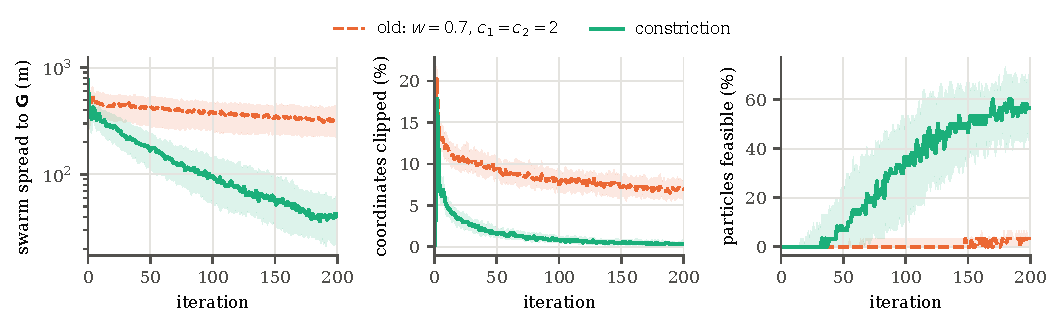
\includegraphics[width=\textwidth]{figures_mpce/diag_pso_dynamics.pdf}
\caption{PSO dynamics with the old setting ($w=0.7$, $c_1=c_2=2$) and the constriction setting on 6 cases $\times$ 10 seeds at 6,030 evaluations (200 iterations): median (line) and interquartile range (band) over the runs. Left: swarm spread, the mean over particles of the RMS distance of the turbines to the global best $\mathbf G$ (log scale). Middle: share of the coordinates that leave the bounding square in an iteration and are clipped (velocities are kept). Right: share of particle evaluations whose layout is feasible. Per-case values: Table~\ref{tab:D-psodyn}.}
\label{fig:D-psodyn}
\end{figure*}

\begin{table*}[!t]
\centering
\caption{PSO dynamics per case, old setting / constriction setting (10 seeds each, 6,030 evaluations). Spread: median over the runs of the swarm spread at the last iteration (m); $|V|$: median mean absolute velocity per coordinate at the last iteration (m); clipped: share of coordinates clipped per iteration (iterations 1--200); feasible, outside, spacing: share of particle evaluations in iterations 101--200 with a feasible layout, with a turbine outside the circle, with two turbines closer than $8R$; $\mathbf G$ feas.: runs whose final global best is feasible; $L$: median wake loss of the feasible final global bests (\%). Note below the table: violations of the infeasible evaluations and of the final layouts of all stored runs of both settings (68 cases $\times$ 30 seeds).}
\label{tab:D-psodyn}
\scriptsize\setlength{\tabcolsep}{3pt}
\begin{tabular}{lcccccccc}
\toprule
Case (DS, $r$, $N$) & Spread (m) & $|V|$ (m) & Clipped (\%) & Feasible (\%) & Outside (\%) & Spacing (\%) & $\mathbf G$ feas. & $L$ (\%) \\
\midrule
I, 500, 6 & 188.9 / 21.7 & 127.7 / 9.5 & 8.8 / 1.9 & 5.8 / 54.8 & 81.0 / 40.6 & 79.3 / 10.6 & 10 / 10 & 0.52 / 0.43 \\
I, 1000, 10 & 436.1 / 58.3 & 268.9 / 21.8 & 8.4 / 1.3 & 3.6 / 66.6 & 87.6 / 23.4 & 85.1 / 17.8 & 10 / 10 & 0.78 / 0.45 \\
I, 750, 12 & 332.1 / 51.4 & 190.5 / 18.6 & 9.1 / 1.6 & 0.7 / 41.9 & 92.9 / 31.1 & 98.8 / 49.0 & 4 / 10 & 3.79 / 1.44 \\
II, 750, 8 & 311.3 / 39.4 & 177.8 / 16.6 & 8.7 / 2.0 & 5.4 / 55.7 & 86.6 / 35.2 & 78.8 / 20.2 & 10 / 10 & 2.67 / 1.82 \\
II, 500, 10 & 197.8 / 14.5 & 125.4 / 4.8 & 8.4 / 1.5 & 0.0 / 27.2 & 89.9 / 36.2 & 100.0 / 64.4 & 0 / 10 & -- / 7.75 \\
II, 1000, 15 & 488.5 / 53.8 & 283.8 / 19.3 & 8.7 / 1.6 & 0.5 / 44.1 & 95.5 / 27.6 & 99.3 / 48.9 & 3 / 10 & 7.13 / 4.94 \\
\midrule
All 6 cases & 319.3 / 40.7 & 187.3 / 15.2 & 8.7 / 1.6 & 2.6 / 48.4 & 88.9 / 32.3 & 90.2 / 35.2 & 37 / 60 & \\
\bottomrule
\end{tabular}
\\[3pt]
\parbox{\textwidth}{\scriptsize Infeasible particle evaluations (iterations 1--200; old / constriction): 98.3 / 68.4\% of all; of these, outside the circle only 5.8 / 18.4\%, spacing only 7.9 / 34.3\%, both 86.3 / 47.3\%. Final layouts of all stored runs (old / constriction; feasibility rule of the paper: a turbine more than $10^{-6}$~m outside the circle, a pair more than $10^{-6}$~m closer than $8R$): infeasible 286 / 0 of 2{,}040; of these, outside the circle only 10 / 0, spacing only 224 / 0, both 52 / 0; with a turbine outside the circle that sits on the box bound at a tangent point ($|x|=r$ or $|y|=r$): 60 / 0. (Spacing from the stored minimum spacing; boundary from the coordinates, which are stored to 1~mm; the 46 old-setting finals whose boundary status is not decidable at 1~mm, or that are among the instrumented runs, are classified with the unrounded positions of the reproduced runs. With a 1-mm tolerance instead, 282 finals are infeasible and 246 violate only the spacing.) Final layouts with a coordinate on the box bound: 68 / 2 (infeasible ones: 60 / 0).}
\end{table*}

\begin{table}[!t]
\centering
\caption{Inside the VNS phase (Phase~2) of the hybrids at 6,030 evaluations: 12 split cases (both data sets; $r=500, 750, 1000$~m with $N=6, 8, 10$ and $N=10, 12, 15$) $\times$ 10 seeds. A cycle is one shaking step followed by the complete local search (compass search); the first descent is the local search from the switch point, before any shaking; every evaluation after it belongs to a cycle. Evaluation shares are pooled over the runs (sum over runs of the evaluations of a stage divided by the sum of the Phase-2 evaluations); medians of the per-run shares are given separately. Improvement shares refer to the reduction of the wake loss in Phase~2 in the runs whose switch point is feasible (pooled); the gain of the cycles includes the local search of a cycle cut off by the budget.}
\label{tab:D-vns}
\scriptsize\setlength{\tabcolsep}{3pt}
\resizebox{\ifdim\width>\columnwidth\columnwidth\else\width\fi}{!}{%
\begin{tabular}{lccc}
\toprule
 & PSO-VNS & SSA-VNS & RS-VNS \\
\midrule
Runs with feasible switch point & 116 of 120 & 100 of 120 & 48 of 120 \\
Phase-2 evaluations (median) & 3{,}000 & 3{,}000 & 3{,}015 \\
First descent: evaluations (median) & 2{,}860 & 2{,}920 & 3{,}015 \\
\quad share of Phase-2 evaluations (pooled, \%) & 78.5 & 75.9 & 84.8 \\
\quad share of Phase-2 evaluations (median over runs, \%) & 95.3 & 97.3 & 100.0 \\
Shake-plus-search cycles: share of Phase-2 evaluations (pooled, \%) & 21.5 & 24.1 & 15.2 \\
\quad in the runs with a feasible switch point (pooled, \%) & 22.3 & 25.8 & 28.1 \\
\quad runs with at least one cycle evaluation & 62 & 62 & 42 \\
Shaking steps per run (median) & 1.0 & 1.0 & 0.0 \\
\quad range over runs & 0--3 & 0--3 & 0--3 \\
\quad median for $N=6$ & 2.0 & 2.0 & 2.0 \\
\quad median for $N=8$ & 1.0 & 1.0 & 1.0 \\
\quad median for $N=10$ & 1.0 & 1.0 & 0.0 \\
\quad median for $N=12$ & 0.0 & 0.0 & 0.0 \\
\quad median for $N=15$ & 0.0 & 0.0 & 0.0 \\
Shaking evaluations (\% of Phase~2; rest: local search) & 0.02 & 0.03 & 0.02 \\
Accepted cycles per run (mean) & 0.1 & 0.1 & 0.1 \\
\quad acceptance rate of cycles (\%) & 22.2 & 25.8 & 80.0 \\
\quad share accepted with $k=1$ (\%) & 100.0 & 100.0 & 100.0 \\
\quad accepted with $k=1,\dots,5$ & 6/0/0/0/0 & 8/0/0/0/0 & 16/0/0/0/0 \\
\quad runs without an accepted cycle & 114 & 112 & 104 \\
\quad shaken point already better (\% of accepted) & 0.0 & 0.0 & 0.0 \\
Improvement from the first descent (pooled, \%) & 97.5 & 90.3 & 88.6 \\
Improvement from accepted cycles (\%) & 0.5 & 3.4 & 3.5 \\
Improvement from all cycles, incl.\ the one cut off (\%) & 2.5 & 9.7 & 11.4 \\
Infeasible at switch, feasible after descent & 1 & 6 & 11 \\
Infeasible at switch, feasible after a cycle & 0 & 0 & 0 \\
Feasible incumbent made infeasible & 0 & 0 & 0 \\
Start is not the best feasible Phase-1 layout$^a$ & 0 & 0 & 0 \\
\bottomrule
\end{tabular}}
\\[2pt]\parbox{\columnwidth}{\scriptsize $^a$ runs in which Phase~1 evaluated at least one feasible layout but handed an infeasible or worse layout to VNS (the penalized comparison picks the best feasible layout whenever one exists).}
\end{table}

\begin{table}[!t]
\centering
\caption{Why PSO (constriction) and DE do not move from feasible starts: the six largest cases and the Horns Rev~1 16-turbine block $\times$ 3 seeds with feasibility-preserving initialization, 6,030 evaluations; every candidate (trial) is logged; feasibility with the 1e-6~m tolerance of the paper. Mixture test: first-update PSO candidates $\mathbf P^i+c_2\,\mathbf r\odot(\mathbf G-\mathbf P^i)$ between a particle's feasible start and the global best (200 draws per particle, separate random stream; $c_2=1.496$, independent $\mathbf r\sim U(0,1)$ per coordinate, clipped to the box), with the original turbine labels and after relabeling the turbines of $\mathbf P^i$ to their nearest turbines of $\mathbf G$ (assignment problem); then, relabelled, without overshoot (weights in $[0,1]$) and with one common weight (a convex combination of the two layouts).}
\label{tab:D-feasstart}
\scriptsize\setlength{\tabcolsep}{3pt}
\resizebox{\ifdim\width>\columnwidth\columnwidth\else\width\fi}{!}{%
\begin{tabular}{lcc}
\toprule
 & PSO & DE \\
\midrule
Runs with an improved global best & 0 of 21 & 0 of 21 \\
Candidates evaluated after the initial population & 126{,}000 & 126{,}000 \\
\quad feasible (\%) & 3.33 & 0.00 \\
\quad feasible, other than re-evaluations of $\mathbf G$ & 0 & 0 \\
Infeasible candidates: outside the site only / spacing only / both (\%) & 0.0 / 3.6 / 96.4 & 0.0 / 0.6 / 99.4 \\
Feasible at the first update (\%) & 3.3 & 0.0 \\
Median min.\ spacing at the first update (m; limit 308, Horns Rev 320) & 95 & 84 \\
Personal-best updates / accepted DE trials & 0 & 0 \\
Feasible candidates better than $\mathbf G$ & 0 & 0 \\
Runs in which the $\mathbf G$-particle keeps $\mathbf V=\mathbf 0$ & 21 of 21 & -- \\
Iterations with exactly one feasible candidate ($\mathbf G$ re-evaluated) & 4{,}200 of 4{,}200 & -- \\
\midrule
\multicolumn{3}{l}{Mixture test (feasible \% / turbine outside the site \% / median min.\ spacing, m):} \\
\quad first PSO move, original labels & \multicolumn{2}{l}{0.0 / 93.1 / 91} \\
\quad first PSO move, relabelled & \multicolumn{2}{l}{0.1 / 80.3 / 189} \\
\quad relabelled, weights in $[0,1]$ & \multicolumn{2}{l}{0.8 / 39.4 / 222} \\
\quad relabelled, one weight (convex comb.) & \multicolumn{2}{l}{16.6 / 0.0 / 286} \\
Initial layouts: RMS turbine distance to $\mathbf G$ after relabeling (m, median / min) & 291 / 111 & \\
\midrule
All stored runs of the paper (30 seeds): final $\ne$ best initial layout & 0 of 210 & 0 of 210 \\
\bottomrule
\end{tabular}}
\end{table}

\begin{table}[!t]
\centering
\caption{Phase~1 of RS-VNS replayed (geometry only, the seeded random stream of the runs): feasible samples among the 3,015 uniform samples in the bounding square, over 30 seeds (90,450 samples per row; the geometry is the same for both data sets). Inside: all $N$ turbines inside the circle, observed rate and $(\pi/4)^N$. Disc: Monte Carlo feasibility rate of the same number of samples uniform in the disc (the Phase-1 distribution of the disc-sampling control RSD-VNS). Rows with $N\le 5$ at 750 and 1000~m omitted (all 30 seeds have feasible samples).}
\label{tab:D-rsreplay}
\scriptsize\setlength{\tabcolsep}{3pt}
\begin{tabular}{rrrrrrr}
\toprule
$r$ (m) & $N$ & feasible & seeds with one & inside (\%) & $(\pi/4)^N$ (\%) & disc feasible (\%) \\
\midrule
500 & 2 & 39{,}952 & 30 & 61.45 & 61.69 & 71.9 \\
500 & 3 & 15{,}525 & 30 & 48.32 & 48.45 & 35.4 \\
500 & 4 & 3{,}740 & 30 & 37.94 & 38.05 & 11.1 \\
500 & 5 & 546 & 30 & 29.76 & 29.88 & 2.11 \\
500 & 6 & 53 & 23 & 23.12 & 23.47 & 0.186 \\
500 & 7 & 1 & 1 & 18.19 & 18.43 & 0.0166 \\
500 & 8 & 0 & 0 & 14.22 & 14.48 & 0 \\
500 & 9 & 0 & 0 & 11.19 & 11.37 & 0 \\
500 & 10 & 0 & 0 & 8.70 & 8.93 & 0 \\
750 & 6 & 1{,}698 & 30 & 23.12 & 23.47 & 8.28 \\
750 & 7 & 458 & 30 & 18.19 & 18.43 & 2.71 \\
750 & 8 & 75 & 25 & 14.22 & 14.48 & 0.711 \\
750 & 9 & 15 & 13 & 11.19 & 11.37 & 0.129 \\
750 & 10 & 2 & 2 & 8.70 & 8.93 & 0.0155 \\
750 & 11 & 0 & 0 & 6.89 & 7.01 & 0.00221 \\
750 & 12 & 0 & 0 & 5.44 & 5.51 & 0 \\
1000 & 6 & 5{,}275 & 30 & 23.12 & 23.47 & 25.1 \\
1000 & 7 & 2{,}264 & 30 & 18.19 & 18.43 & 14.1 \\
1000 & 8 & 906 & 30 & 14.22 & 14.48 & 7.03 \\
1000 & 9 & 280 & 30 & 11.19 & 11.37 & 3.11 \\
1000 & 10 & 101 & 27 & 8.70 & 8.93 & 1.25 \\
1000 & 11 & 23 & 15 & 6.89 & 7.01 & 0.385 \\
1000 & 12 & 8 & 8 & 5.44 & 5.51 & 0.138 \\
1000 & 13 & 1 & 1 & 4.21 & 4.33 & 0.0376 \\
1000 & 14 & 0 & 0 & 3.26 & 3.40 & 0.00663 \\
1000 & 15 & 0 & 0 & 2.64 & 2.67 & 0.00111 \\
\bottomrule
\end{tabular}
\end{table}



\subsection{PSO Dynamics of the Two Settings}
\label{sec:S-diag-pso}
Fig.~\ref{fig:D-psodyn} and Table~\ref{tab:D-psodyn} compare the old and the constriction setting on \NDDynCases{} cases $\times$ \NDDynSeeds{} seeds. At the last iteration, the swarm of the old setting is \NDSpreadRatio{} times as wide and its mean absolute velocity \NDVelRatio{} times as large as with the constriction setting: it contracts much less, consistent with its missing order-2 stability (Proposition~\ref{prop:S-settings}; Section~\ref{sec:S-csweep}). It clips \NDClipOld\% of the coordinates per iteration (constriction: \NDClipNew\%), and only \NDFeasPartOld\% of its particle evaluations in iterations 101--200 are feasible (constriction: \NDFeasPartNew\%). % CHECK-DIAG [D03]-[D05]
Most of its infeasible evaluations violate both constraints. The infeasible \emph{final} layouts, however, mostly violate only the spacing constraint: with the $10^{-6}$~m rule of the paper, \NDStoredSpacingOnlyOld{} of the \NDStoredInfeasOld{} infeasible final layouts of the old setting violate only the spacing, \NDStoredBoundOnlyOld{} only the boundary and \NDStoredBothOld{} both. In $F_p$~\eqref{M-eq:penalty}, the boundary violation $g^{\rm b}_i=x_i^2+y_i^2-r^2$ is measured in m$^2$ and the spacing violation $g^{\rm s}_{ij}$ in m, so a turbine clearly outside the circle is penalized much more than two turbines slightly too close, and the best infeasible layout tends to lie inside the circle with turbines too close. The remaining boundary violations are mostly a penalty-scaling effect as well: in \NDStoredTangentOld{} of the \NDStoredAnyBoundOld{} final layouts that violate the boundary, an outside turbine is pinned at the box, near a point where the box touches the circle (one coordinate at $\pm r$), where $g^{\rm b}_i=y_i^2$ is of second order in the other coordinate and hence cheap in $F_p$. Normalized violations remove the mixed units but not the second effect: under Deb's rules on $g^{\rm b}_i/r^2$ and $g^{\rm s}_{ij}/\ell_{\min}$ with box clipping, PSO ends with turbines outside the circle more often (Section~\ref{sec:S-sa-constraint}). The infeasibility of the final layouts of the old setting is therefore mainly a spacing problem, not one of turbines left outside the circle. % CHECK-DIAG [D06], [D07], [D21]

\subsection{Inside the VNS Phase}
\label{sec:S-diag-vns}
Table~\ref{tab:D-vns} follows Phase~2 of PSO-VNS, SSA-VNS and RS-VNS on the \NDVnsCases{} cases of the split study $\times$ \NDVnsSeeds{} seeds. At 6,030 evaluations, Phase~2 is essentially one compass-search descent: for PSO-VNS, the first descent from the switch point takes a median of \NDDescentEvalsPSOVNS{} evaluations (pooled share \NDDescentEvalsPctPSOVNS\% of the Phase-2 evaluations; median share per run \NDDescentEvalsPctMedianPSOVNS\%) and yields \NDDescentSharePSOVNS\% of the Phase-2 improvement, and \NDNoAcceptedPSOVNS{} of \NDVnsRunsPSOVNS{} runs have no accepted shaking cycle. A shake costs a single evaluation; the relevant cost is that of the cycles (shake plus the local search that follows it), which take \NDCycleEvalsPctPSOVNS\% of the Phase-2 evaluations (pooled; median run \NDCycleEvalsPctMedianPSOVNS\%) and give \NDCycleSharePSOVNS\% of the Phase-2 gain (\NDCycleAllSharePSOVNS\% including the cycle cut off by the budget). % CHECK-DIAG [D08], [D20]
For $N\ge12$ the median run has no shaking step at all, because the first descent almost never finishes within the budget, and all accepted cycles use the smallest neighbourhood $k=1$. % CHECK-DIAG [D09], [D10]
VNS never makes a feasible incumbent infeasible, and its start is always the best feasible Phase-1 layout when Phase~1 evaluated one. % CHECK-DIAG [D11], [D12]
The component analysis (Section~\ref{M-sec:ablation}) therefore measures the value of a local-search phase after Phase~1, a truncated best-improvement compass search at this budget; the neighbourhood structure of VNS can matter only for small $N$, and the local-minimality certificate of Proposition~\ref{prop:S-ls} does not apply to the runs in which the first descent is unfinished.

\subsection{Feasible Starts}
\label{sec:S-diag-feas}
Table~\ref{tab:D-feasstart} logs every candidate of PSO and DE from feasible starts (\NDFsCases{} cases $\times$ \NDFsSeeds{} seeds). Neither method improves on the best initial layout, in these runs or in any of the \NDFsStoredRunsPSO{} stored runs of each. % CHECK-DIAG [D13]
Of the \NDFsCandPSO{} PSO candidates, \NDFsFeasCandPSO\% are feasible, and every one of them is the particle holding $\mathbf G$ (with zero velocity) re-evaluating $\mathbf G$, as in Proposition~\ref{prop:S-frozen}(a); no personal best is ever updated, and none of the \NDFsCandDE{} DE trials is feasible or accepted. % CHECK-DIAG [D14]
Label symmetry does not explain the stall: after the turbines of each start are relabelled to their nearest turbines of $\mathbf G$, the first PSO move is still feasible in only \NDFsMixMatched\% of the draws, and only a common weight for all coordinates (a convex combination of two layouts) gives \NDFsMixScalar\%. % CHECK-DIAG [D15]
The feasible starts are distinct dense layouts (median RMS turbine distance to $\mathbf G$ after relabeling \NDFsInitRms~m), and the independent per-coordinate weights, with overshoot beyond $\mathbf G$, place turbines too close to each other or outside the site. % CHECK-DIAG [D16]

\subsection{Phase~1 of RS-VNS}
\label{sec:S-diag-rs}
Table~\ref{tab:D-rsreplay} replays the random stream of Phase~1 of RS-VNS. The replay agrees with the stored runs, and the share of samples with all turbines inside the circle matches $(\pi/4)^N$ (Proposition~\ref{M-prop:S-box} of the main text). In \NDRsRunsNoFeasSample{} RS-VNS runs, among them all runs of \NDRsCasesNoFeasSample{} cases, Phase~1 draws no feasible layout at all, and VNS starts from the least-violating sample (Section~\ref{sec:S-th-budget}); in all of these runs the spacing constraint is binding (Section~\ref{sec:S-ablation}). The last column of Table~\ref{tab:D-rsreplay} gives the feasibility rate of samples drawn uniformly in the disc, the Phase-1 distribution of the control RSD-VNS (Section~\ref{sec:S-ablation}). % CHECK-DIAG [D17]

\section{Published Kusiak--Song Results}
\label{sec:S-literature}
The Kusiak--Song benchmark has been solved with an evolution strategy~\cite{Kusiak2010}, ant colony optimization~\cite{Eroglu2012}, particle filtering~\cite{Eroglu2013} and biogeography-based optimization~\cite{Bansal2017}. We do not compare our results numerically with these studies. The published values available to us are transcriptions whose source tables could not be checked against the original papers, several of them are internally inconsistent (e.g., objective and wake loss that do not add up to the wake-free value), and the budgets, the numbers of runs and the handling of infeasible layouts of these studies differ from ours or are not reported. The transcribed values and the status of each are listed in \texttt{analysis/literature\_values.csv} and \texttt{analysis/literature\_values.md}.
% AUTHOR: if the published values are verified against the original papers, a comparison table can be added here.

\section{Reproducibility Map}
\label{sec:S-repro}
This map lists the script that produces each part of the results. All scripts, run records and generated outputs are contained in the reproducibility package (Data availability of the main text); its README gives, for every table, figure and number of the article, the command, the input files and the run time, and for every optimization study the exact command and shard layout. The complete analysis pipeline was re-executed from the package in the environment of the runs (CPython 3.11.15, NumPy 2.4.6, SciPy 1.17.1, pandas 3.0.6, Matplotlib 3.11.2): all 91 regenerated or compared outputs are byte-identical to the stored pipeline outputs or differ only in generation time stamps, PDF creation dates and recorded software versions, and all automated checks pass (Section~\ref{sec:S-archive}). Re-executed in this validation were the analysis pipeline, a determinism sample of stored runs (one record per study, site kind and method) and the full-precision reruns of Section~\ref{sec:S-sa-precision}; not re-executed were the optimization runs themselves, the instrumented diagnostic reruns and the calibration reruns of the original code (Section~\ref{sec:S-archive}). The package (release 1.0.0: \texttt{SWEVO\_repro\_1.0.0.zip} with the checksum list \texttt{MANIFEST.sha256} and a README) is supplied to the editors and reviewers with the submission and will be deposited publicly with a DOI upon acceptance.

Table~\ref{tab:S-repro} gives the map (commands and order of the calls: \texttt{analysis/README\_reproduce.md}). The per-run results of the main comparison come from two generations of experiment scripts with the same objective and optimizer code: SSA, LX-SSA, DE, the old-setting PSO, VNS, SSA-VNS and LX-SSA-VNS from the grid scripts of a preliminary comparison of ours (\texttt{fresh\_*.csv}), and PSO, PSO-VNS, RS-VNS, RSD-VNS and MS-SLSQP, as well as the split, initialization, budget, Horns Rev~1 and IEA37 studies, from \texttt{analysis/mpce\_experiments.py} and \texttt{analysis/iea37\_experiments.py} (\texttt{mpce\_*.csv}); \texttt{mpce\_results.py} records the source file of every run. Reruns of stored runs of the gradient-free methods with the archived drivers reproduce the records bit for bit (or to floating-point noise) in every field except the elapsed time; SLSQP-based runs are not bit-reproducible across CPU and BLAS builds (Section~\ref{sec:S-sa-precision}). Convergence curves are stored at every $\lfloor(B-30)/200\rfloor$ evaluations.\IfSuppTable{tab:provenance}{ Table~\ref{tab:provenance} gives the source of the runs of every method and study.}{}
\begin{table}[!htb]
\centering
\caption{Reproducibility map: script (in \texttt{analysis/}) that produces each part of the results. Commands and run files: \texttt{analysis/README\_reproduce.md}.}
\label{tab:S-repro}
\footnotesize\setlength{\tabcolsep}{4pt}
\begin{tabular}{>{\raggedright\arraybackslash}p{0.42\textwidth}>{\raggedright\arraybackslash}p{0.52\textwidth}}
\toprule
Results & Script \\
\midrule
Runs of PSO, PSO-VNS, RS-VNS, RSD-VNS, MS-SLSQP; split, feasible-initialization, budget and Horns Rev~1 studies & \texttt{mpce\_experiments.py} (one experiment id per study) \\
Runs of IEA37 Case Study~1 & \texttt{iea37\_experiments.py} \\
Runs of SSA, LX-SSA, DE, old-setting PSO, VNS, SSA-VNS, LX-SSA-VNS & \texttt{full\_grid\_experiments.py} of a preliminary comparison of ours, experiments \texttt{grid} (SSA, LX-SSA, DE, old-setting PSO), \texttt{vgrid} (VNS) and \texttt{bgrid} (SSA-VNS, LX-SSA-VNS) \\
Main-text tables, generated tables of this document (\texttt{mpce\_supplementary.tex}), figures in \texttt{figures\_mpce/}, \texttt{mpce\_summary.json} & \texttt{mpce\_results.py} (called by \texttt{build\_mpce\_paper.sh}) \\
Number macros \texttt{mpce\_numbers.tex}; checks of outcome-dependent statements & \texttt{mpce\_numbers.py}; \texttt{mpce\_check\_final.py} (both called by \texttt{mpce\_results.py}) \\
Re-evaluation with the cubic power curve and the Gaussian wake & \texttt{mpce\_robustness.py} (cached in \texttt{mpce\_reevaluation\_cache.csv}) \\
Spacing re-optimization with SSA and LX-SSA (Table~\ref{tab:spacing-authors}) & \texttt{analyze\_authors\_runs.py} \\
Spacing re-optimization of the nine methods at $5D$ and $6D$ (Section~\ref{sec:S-xp-spacing}) & runs: \texttt{rev2\_spacing.py}; statistics and tables: \texttt{rev2\_analysis.py} \\
Exact-gradient baselines on IEA37 (Section~\ref{sec:S-xp-grad}) & runs, gradient check and $c_g$: \texttt{rev2\_gradient.py} (with \texttt{check}); statistics and tables: \texttt{rev2\_analysis.py} \\
Second site, Lillgrund block (Section~\ref{sec:S-xp-site}) & model and PyWake check: \texttt{rev2\_site\_model.py} (with \texttt{--pywake}); runs: \texttt{rev2\_site.py}; statistics and table: \texttt{rev2\_analysis.py} \\
Packing capacity (Table~\ref{tab:capacity}) & \texttt{packing\_capacity.py} \\
Model schematics (Fig.~\ref{M-fig:model} of the main text) & \texttt{make\_model\_figures.py} \\
Verification of the evaluator against the original code and archived runs; IEA37 calculator & \texttt{validate\_evaluator.py}, \texttt{calibrate\_authors\_code.py}; \texttt{iea37\_model.py} (run as a script) \\
Robustness of the statistical conclusions, equivalence at three levels, equivalence curve (Section~\ref{sec:S-inference}, Fig.~\ref{M-fig:equiv-curve} of the main text); \texttt{mpce\_numbers\_extra.tex} & \texttt{mpce\_inference\_extra.py} and \texttt{mpce\_check\_extra.py} (checks X01--X57), after \texttt{mpce\_results.py} \\
Algorithm diagnostics (Section~\ref{sec:S-diag}); \texttt{mpce\_numbers\_diag.tex}, \texttt{diag\_*.pdf} & \texttt{mpce\_diagnostics.py} (instrumented reruns, about 18~min; run separately) and \texttt{mpce\_check\_diag.py} (checks D01--D22) \\
PSO coefficient sweep and bound handling (Section~\ref{sec:S-csweep}); \texttt{mpce\_numbers\_csweep.tex}, \texttt{csweep.pdf} & runs: \texttt{mpce\_experiments.py}; analysis: \texttt{mpce\_csweep.py} and \texttt{mpce\_check\_csweep.py} (checks S01--S15) \\
Direction resolution, Horns Rev~1 re-evaluation and PyWake check, projected IEA37 layouts (Sections~\ref{sec:S-hr16}, \ref{sec:S-iea37} and~\ref{sec:S-direction}); \texttt{mpce\_numbers\_dir.tex} & \texttt{mpce\_direction.py}, \texttt{pywake\_check.py} (PyWake~\NFPyWakeVersion), \texttt{iea37\_projected.py}; \texttt{mpce\_check\_dir.py} (checks F01--F46) \\
Theoretical details (Section~\ref{sec:S-theory}), \texttt{theory\_*.pdf} & \texttt{make\_theory\_figures.py}; with \texttt{--check} (about 3~min) it verifies every number of Section~\ref{sec:S-theory} (checks T01--T13) \\
Laplace ablation and real-coded GA (Section~\ref{sec:S-xp-lap}) & runs: \texttt{rev2\_laplace.py}, \texttt{rev2\_ga.py}; statistics and tables: \texttt{rev2\_analysis.py} (reuses the functions of \texttt{mpce\_results.py} and \texttt{mpce\_inference\_extra.py}) \\
Sensitivity analyses and experiments (Section~\ref{sec:S-sa}) & \texttt{rev3\_inference.py}, \texttt{rev3\_sites.py}; runs and analysis: \texttt{rev3\_constraint.py} and \texttt{rev3\_constraint\_analysis.py}, \texttt{rev3\_fine.py} and \texttt{rev3\_fine\_analysis.py}; coordinate audit: \texttt{rev3\_precision\_audit.py}, \texttt{rev3\_precision\_rerun.py} \\
Archive audit and Lillgrund all-run endpoint (Section~\ref{sec:S-archive}) & \texttt{audit\_archive.py} \\
\bottomrule
\end{tabular}
\end{table}
\SuppTableOpt{tab:provenance}
% flush the reproducibility map and the provenance table onto their own page before the references: forced out by the
% \FloatBarrier of the bibliography heading (placeins), they overfilled the text page by 5.7 pt
\clearpage

\section{Additional Experiments: Laplace Ablation, a Real-Coded GA, Minimum Spacing, Exact Gradients and a Second Site}
\label{sec:S-xp-lap}
This section reports five additional experiments: an ablation of the Laplace step of LX-SSA (Section~\ref{sec:S-xp-lap-abl}), a real-coded genetic algorithm as a ninth method of the main comparison (Section~\ref{sec:S-xp-ga}), a re-optimization at minimum spacings $5D$ and $6D$ (Section~\ref{sec:S-xp-spacing}), exact-gradient baselines on IEA37 Case Study~1 (Section~\ref{sec:S-xp-grad}) and a second site with a measured wind climate, a Lillgrund block (Section~\ref{sec:S-xp-site}). These experiments were designed after the main comparison. The first three use the penalized objective~\eqref{M-eq:penalty}, the bounds, the counting of evaluations, the seeds 1--30 and the random initialization of the main comparison, and the statistics of Section~\ref{sec:S-stats}: wake loss in \% of the wake-free objective, feasibility-aware ranking with qualification at 15 of 30 feasible runs, case-mean Wilcoxon tests with Holm's correction, and 90\% percentile bootstrap intervals over the cases (10{,}000 resamples) with the margin of 0.05~pp of Table~\ref{tab:equivalence}; the exact-gradient methods use the constrained formulation of MS-SLSQP (Section~\ref{sec:S-slsqp}), the same seeds and random initialization, and are compared at the run level, as are the methods on the Lillgrund block, which follows the Horns Rev~1 protocol (Sections~\ref{sec:S-hrmodel} and~\ref{sec:S-hr16}). No table or number of the main text depends on these experiments, except those that cite this section.

\subsection{Laplace Ablation}
\label{sec:S-xp-lap-abl}
LX-SSA as published differs from SSA in two respects (Section~\ref{M-sec:ssa} and Algorithm~\ref{alg:S-ssa}): every follower also evaluates a Laplace candidate~\eqref{M-eq:laplace} and keeps the better of it and the SSA midpoint, and an iteration costs $2N_p$ evaluations instead of $N_p$, partly because the kept candidates are evaluated again with the whole population. Six variants separate these components. Each was run on the 12 cases of the split study (middle and largest $N$ per farm and data set; Table~\ref{M-tab:design}) with 30 seed-paired runs of 6{,}030 evaluations from random starts (2{,}160 runs); SSA and LX-SSA ($\chi=1$) are the stored runs of the main comparison. \emph{No re-evaluation}: LX-SSA without the redundant re-evaluation; the leaders are evaluated once and every follower keeps the known value of its chosen candidate, so an iteration costs $1.5N_p=45$ evaluations (133 full iterations and a 134th in which only the leaders are evaluated, exactly 6{,}030 evaluations); with the same number of iterations, its trajectory is that of LX-SSA. \emph{Laplace replaces midpoint}: every follower takes the Laplace candidate instead of the midpoint, without comparison, at the cost of SSA ($N_p$ evaluations per iteration, 200 iterations). \emph{Uniform $\gamma$}: LX-SSA as published with $\gamma\sim U(-2,2)$ instead of the Laplace distribution; like Laplace$(0,1)$, it is symmetric about zero with $\mathrm E\lvert\gamma\rvert=1$, but it is light-tailed ($\lvert\gamma\rvert\le2$), so it isolates the heavy tail. \emph{Scale}: LX-SSA as published with $\chi=0.25$, 0.5 and 2 ($\phi=0$).

Table~\ref{tab:S-xp-laplace} gives the results. The eight methods differ (Friedman $\chi^2_F=38.2$, 7 d.f., $p=2.72\times10^{-6}$). SSA and LX-SSA have at least 15 feasible runs in 10 of the 12 cases, so the loss differences are taken over these 10 cases; there, LX-SSA has a mean wake loss 0.246~pp higher than SSA (90\% CI [0.103, 0.396]).
\emph{Cost.} Without the re-evaluation, LX-SSA has a 0.169~pp lower mean wake loss ([$-$0.293, $-$0.060]; lower in 8 of the 10 cases) but remains 0.077~pp above SSA ([0.018, 0.144]): part of the deficit of LX-SSA is its doubled evaluation cost.
\emph{Laplace step vs.\ midpoint.} At the cost of SSA, the variant with the Laplace candidate in place of the midpoint is feasible in more runs than SSA (93.9\% vs.\ 90.0\%; at least 15 feasible runs in all 12 cases vs.\ 10) and ranks first alone in 6 cases (SSA: 4), but in the 10 cases in which both qualify its mean wake loss is 0.077~pp higher ([$-$0.029, 0.189]; 3.149\% vs.\ 3.073\%), and its average rank, 2.83, is close to that of SSA, 2.67. The Laplace step thus gives no advantage in wake loss over the SSA midpoint.
\emph{Heavy tail.} With the uniform $\gamma$, the mean wake loss is that of LX-SSA within 0.007~pp ([$-$0.073, 0.052]): the heavy tail of the Laplace distribution has no detectable effect, although equivalence within $\pm0.05$~pp is not shown.
\emph{Scale.} Smaller scales are worse: $\chi=0.25$ and $\chi=0.5$ raise the mean wake loss of LX-SSA by 0.155~pp ([0.073, 0.243]) and 0.093~pp ([0.012, 0.170]) and have the two worst average ranks (7.42 and 6.33). With $\chi=2$ the loss is 0.123~pp lower ([$-$0.263, 0.009], an interval that includes zero; average rank 3.92 vs.\ 4.25), but still 0.122~pp above SSA ([0.048, 0.200]); no tested scale brings LX-SSA level with SSA.

With 12 cases, the case-level tests have little power. None of the Holm-adjusted case-mean Wilcoxon tests against LX-SSA is significant (smallest $p_{\rm Holm}=0.085$), and against SSA only $\chi=0.25$ is (worse, $p_{\rm Holm}=0.014$). In the Holm-adjusted average-rank tests, $\chi=0.25$ ranks worse than LX-SSA ($p=0.011$), and $\chi=0.25$ and $\chi=0.5$ rank worse than SSA, the best-ranked method ($p=1.4\times10^{-5}$ and $p=0.0015$); no other rank difference is significant. With the cases fixed (seed-level bootstrap within cases), the 90\% intervals mostly give the same reading, e.g., [$-$0.259, $-$0.079]~pp for the variant without re-evaluation and [$-$0.101, 0.087]~pp for the uniform $\gamma$, both against LX-SSA; they differ on whether zero is excluded for $\chi=0.5$ ([$-$0.013, 0.206]) and $\chi=2$ ([$-$0.215, $-$0.032]) against LX-SSA and for the variant without re-evaluation against SSA ([$-$0.004, 0.158]). The differences above are therefore estimates with their intervals, not confirmed effects. On these cases, the Laplace step gives LX-SSA no advantage over the SSA midpoint, part of its deficit against SSA is its doubled evaluation cost, the heavy tail does not matter, and scales below the published $\chi=1$ are worse.

\begin{table}[!htbp]
\centering
\caption{Role and parameterization of the Laplace step: SSA, LX-SSA and six LX-SSA variants on the 12 cases of the split study (6{,}030 evaluations, 30 seed-paired runs).}
\label{tab:S-xp-laplace}
\scriptsize\setlength{\tabcolsep}{2pt}
\begin{tabular}{lcccccccccc}
\toprule
& & & & & \multicolumn{3}{c}{vs.\ LX-SSA} & \multicolumn{3}{c}{vs.\ SSA} \\
\cmidrule(lr){6-8}\cmidrule(lr){9-11}
Method & Calls/it. / $T$ & Loss (\%) & Feas. & Rank & $\overline{\Delta L}$ & 90\% CI & $p_{\rm Holm}$ & $\overline{\Delta L}$ & 90\% CI & $p_{\rm Holm}$ \\
\midrule
SSA & 30 / 200 & 3.073$^{10}$ & 90.0 & 2.67 & $-$0.246 & [$-$0.396, $-$0.103] & 0.195 & -- & -- & -- \\
LX-SSA & 60 / 100 & 3.319$^{10}$ & 88.9 & 4.25 & -- & -- & -- & +0.246 & [0.103, 0.396] & 0.148 \\
LX-SSA, no re-evaluation & 45 / 134 & 3.150$^{10}$ & 88.9 & 3.75 & $-$0.169 & [$-$0.293, $-$0.060] & 0.186 & +0.077 & [0.018, 0.144] & 0.168 \\
LX-SSA, Laplace replaces midpoint & 30 / 200 & 3.979 & 93.9 & 2.83 & $-$0.169 & [$-$0.297, $-$0.057] & 0.085 & +0.077 & [$-$0.029, 0.189] & 0.891 \\
LX-SSA, $\gamma\sim U(-2,2)$ & 60 / 100 & 3.311$^{10}$ & 89.4 & 4.83 & $-$0.007 & [$-$0.073, 0.052] & 0.922 & +0.238 & [0.108, 0.377] & 0.059 \\
LX-SSA, $\chi=0.25$ & 60 / 100 & 3.474$^{10}$ & 86.7 & 7.42 & +0.155 & [0.073, 0.243] & 0.117 & +0.401 & [0.243, 0.572] & 0.014 \\
LX-SSA, $\chi=0.5$ & 60 / 100 & 3.412$^{10}$ & 85.0 & 6.33 & +0.093 & [0.012, 0.170] & 0.316 & +0.339 & [0.152, 0.537] & 0.059 \\
LX-SSA, $\chi=2$ & 60 / 100 & 3.195$^{10}$ & 90.0 & 3.92 & $-$0.123 & [$-$0.263, 0.009] & 0.465 & +0.122 & [0.048, 0.200] & 0.148 \\
\bottomrule
\end{tabular}
\par\vspace{2pt}\parbox{\textwidth}{\scriptsize Calls/it.\ / $T$: objective evaluations per iteration and number of iterations at 6{,}030 evaluations. Loss: mean wake loss (\%) of the feasible runs, averaged over the cases in which the method has at least 15 feasible runs of 30 (superscript: number of such cases when fewer than 12; the variant with the Laplace candidate in place of the midpoint qualifies in all 12 cases, and its mean over the 10 cases of the other methods is 3.149\%). Feas.: feasible runs (\%). Rank: average feasibility-aware rank among the 8 methods of this table. $\overline{\Delta L}$: mean difference of the per-case mean wake losses, method minus reference (pp; negative = method better) over the cases in which both qualify, with 90\% percentile bootstrap CI over the cases; $p_{\rm Holm}$: case-mean Wilcoxon signed-rank test, Holm-adjusted over the 7 comparisons with the same reference. LX-SSA and SSA: stored runs of the main comparison. Friedman $\chi^2_F=38.2$ (7 d.f.), $p=2.72\times10^{-6}$; Iman--Davenport $F_F=9.2$, $p=3.25\times10^{-8}$.}
\end{table}

\subsection{Real-Coded Genetic Algorithm}
\label{sec:S-xp-ga}
A standard real-coded GA (label GA) was run on the 68 benchmark cases with 30 seed-paired runs of 6{,}030 evaluations from random starts (2{,}040 runs): $N_p=30$, binary tournament selection, simulated binary crossover (SBX)~\cite{Deb1995} ($\eta_c=15$, $p_c=0.9$, per-variable exchange probability 0.5), polynomial mutation~\cite{DebGoyal1996} ($\eta_m=20$, $p_m=1/n$ with $n=2N$ variables), clipping to the box, and generational replacement with elitism. The initial population and every generation cost $N_p$ evaluations (200 generations). These are common default settings, not tuned to this benchmark. GA minimizes the same penalized objective as the other penalty-based methods, with the same evaluation counting; the runs of the other eight methods are those of the main comparison. The comparison covers the 68 benchmark cases, the Horns Rev~1 block and IEA37 Case Study~1 (see below).
% GA Horns Rev 1 / IEA37: rev2_gahr (60 runs) and rev2_gaiea (120 runs) complete; reported below (tab:S-xp-ga-hr, tab:S-xp-ga-iea; numbers from rev2out_ga/rev2_summary.json: ga_hr16, ga_iea37).

Table~\ref{tab:S-xp-ga} gives the case-level analysis of the nine methods (Friedman $\chi^2_F=374.8$, 8 d.f., $p=4.46\times10^{-76}$). GA ranks third (average rank 2.74) after PSO-VNS (2.18) and PSO (2.40), and alone ranks first in 16 cases (PSO-VNS: 21, PSO: 17). It differs significantly from neither PSO-VNS nor PSO, in the average-rank test (Holm $p=0.468$ and $0.471$) or in the case-mean Wilcoxon test ($p_{\rm Holm}=0.101$ and $0.696$). Its mean wake loss is 0.026~pp higher than that of PSO-VNS (90\% CI [$-$0.006, 0.062]) and 0.008~pp higher than that of PSO ([$-$0.022, 0.041]): GA and PSO are practically equivalent at the 0.05~pp margin ($p_{\rm TOST}=0.020$, $m_{\min}=0.041$~pp), whereas equivalence of GA and PSO-VNS is not shown ($m_{\min}=0.062$~pp). At the run level, GA is significantly worse than PSO-VNS in 8 cases and better in 1 (PSO: 5 and 2), and it is feasible in 98.6\% of its runs (PSO-VNS and PSO: 100\%). Against the other six methods, GA has a lower mean wake loss, by 0.305~pp (SSA-VNS) to 0.857~pp (DE), with 90\% intervals wholly below zero; it is significantly better in 39 (SSA-VNS) to 58 (SSA) cases and worse in at most 3, and all Holm-adjusted $p$ values are at most 0.002.

The relative order of the other eight methods is unchanged, and without GA their average ranks are those of Table~\ref{M-tab:friedman68}; the eight-method analysis of the main text therefore stands. In the nine-method pool, PSO-VNS keeps the best average rank, and a standard real-coded GA performs about as well as PSO on this benchmark and better than the salp-swarm methods, VNS, MS-SLSQP and DE.

\emph{Horns Rev~1 and IEA37.} GA was also run, with the same settings and random starts, on the Horns Rev~1 block (Section~\ref{M-sec:hornsrev-site}) and on the 16- and 36-turbine scenarios of IEA37 Case Study~1 (Section~\ref{M-sec:iea37}), with 30 seeds at 6{,}030 and 30{,}030 evaluations (200 and 1{,}000 generations; 60 and 120 runs); the other methods are the stored runs of the main text (Tables~\ref{tab:S-xp-ga-hr} and~\ref{tab:S-xp-ga-iea}). On the Horns Rev~1 block, GA is feasible in 30 of 30 runs at both budgets. At 6{,}030 evaluations its mean AEP loss, 7.18\% (mean AEP 138.12~GWh/yr), is the second lowest, after that of PSO-VNS (7.07\%); in seed-paired Wilcoxon tests (infeasible runs below every feasible run, Holm over the ten comparisons of GA), GA does not differ significantly from PSO-VNS ($p_{\rm Holm}=0.53$) and is better than each of the other nine methods ($p_{\rm Holm}\le0.013$). At 30{,}030 evaluations GA has the lowest mean AEP loss of all methods, 6.16\% (139.64~GWh/yr), against 6.52\% for PSO-VNS, 6.78\% for PSO (28 feasible runs) and 6.85\% for VNS, and it is better than each of the other ten methods ($p_{\rm Holm}\le1.1\times10^{-4}$, the largest against PSO-VNS). With the 5$^\circ$ bins used in optimization, 6 of its 30 layouts at this budget exceed the AEP of the installed block (PSO-VNS: 3); re-evaluated with 1$^\circ$ bins and with PyWake, GA keeps its lead at this budget (Table~\ref{tab:S-sa-hr-eval}; all methods in one pool: Table~\ref{tab:S-sa-hr-pool}).

On IEA37, all 120 GA runs are feasible. With 16 turbines, the mean AEP of GA is the second highest at both budgets (391{,}037.6 and 401{,}766.1~MWh; PSO-VNS: 395{,}031.8 and 402{,}583.1~MWh), and its best runs (399{,}691.3 and 409{,}194.2~MWh) are below those of PSO-VNS, PSO and MS-SLSQP (at 6{,}030 evaluations also below those of SSA-VNS, 403{,}251.3, and VNS, 400{,}169.3~MWh). With 36 turbines, GA has the highest best-run AEP and the highest mean AEP of the methods of Table~\ref{tab:S-xp-ga-iea} and Table~\ref{tab:iea37-detail} at both budgets (the exact-gradient methods of Section~\ref{sec:S-xp-grad} are higher) (best 795{,}530.1 and 836{,}526.4~MWh; mean 774{,}971.9 and 823{,}061.5~MWh, against the next highest means of 741{,}565.6~MWh for VNS at 6{,}030 and 807{,}446.0~MWh for PSO-VNS at 30{,}030 evaluations); its best layout at 30{,}030 evaluations lies 3.14\% below the best feasible published layout in AEP (5.20\% after radial projection; PSO-VNS: 4.20\% and 6.23\%). Beyond the benchmark, GA thus gains more from the larger budget than PSO-VNS on the Horns Rev~1 block and is the strongest of the gradient-free methods compared with 36 IEA37 turbines. These runs cover one site and one case study with 30 seeds each; they do not change the benchmark ranking of Table~\ref{tab:S-xp-ga}, but show that it need not hold beyond the benchmark.

\begin{table}[!htbp]
\centering
\caption{Real-coded genetic algorithm (GA) added to the method pool: case-level analysis of the nine methods over the 68 benchmark cases (6{,}030 evaluations, 30 seed-paired runs).}
\label{tab:S-xp-ga}
\scriptsize\setlength{\tabcolsep}{2.5pt}
\begin{tabular}{lcccccccc}
\toprule
Method & Avg.\ rank & Best & Feas. & $p_z$ & $p_W$ & $\overline{\Delta L}$ (GA $-$ method) & 90\% CI & W/T/L (GA) \\
\midrule
PSO-VNS & 2.18 & 21 & 100.0 & 0.468 & 0.101 & +0.026 & [$-$0.006, 0.062] & 1/59/8 \\
PSO & 2.40 & 17 & 100.0 & 0.471 & 0.696 & +0.008 & [$-$0.022, 0.041] & 2/61/5 \\
GA & 2.74 & 16 & 98.6 & -- & -- & -- & -- & -- \\
SSA-VNS & 4.32 & 0 & 99.6 & 0.002 & $9.29\times10^{-10}$ & $-$0.305 & [$-$0.376, $-$0.237] & 39/28/1 \\
VNS & 5.21 & 3 & 100.0 & $5.28\times10^{-7}$ & $1.07\times10^{-9}$ & $-$0.439 & [$-$0.522, $-$0.359] & 46/19/3 \\
SSA & 6.34 & 0 & 97.6 & $8.52\times10^{-14}$ & $6.06\times10^{-11}$ & $-$0.609 & [$-$0.742, $-$0.483] & 58/10/0 \\
MS-SLSQP & 6.85 & 1 & 100.0 & $1.10\times10^{-17}$ & $2.34\times10^{-10}$ & $-$0.410 & [$-$0.483, $-$0.334] & 56/10/2 \\
LX-SSA & 7.01 & 0 & 96.9 & $5.68\times10^{-19}$ & $6.06\times10^{-11}$ & $-$0.762 & [$-$0.937, $-$0.597] & 57/11/0 \\
DE & 7.96 & 0 & 71.4 & $8.44\times10^{-28}$ & $1.14\times10^{-10}$ & $-$0.857 & [$-$1.103, $-$0.622] & 55/13/0 \\
\bottomrule
\end{tabular}
\par\vspace{2pt}\parbox{\textwidth}{\scriptsize Avg.\ rank: average feasibility-aware rank among the nine methods (rule of Table~\ref{M-tab:friedman68}); Best: cases in which the method alone ranks first; Feas.: feasible runs (\%); $p_z$: Holm-adjusted $p$ of the average-rank test against GA; $p_W$: Wilcoxon signed-rank test on the per-case mean wake losses, GA vs.\ the method (Holm-adjusted over the 8 methods; cases in which only one qualifies imputed); $\overline{\Delta L}$: mean difference of the case-mean wake losses, GA minus method (pp; positive = GA worse), over the cases in which both have at least 15 feasible runs, 90\% bootstrap CI over the cases; W/T/L: cases in which GA is significantly better / not different / worse (seed-paired Wilcoxon, Holm over the 8 comparisons of GA in each case). Friedman $\chi^2_F=374.8$ (8 d.f.), $p=4.46\times10^{-76}$; Iman--Davenport $F_F=148.5$, $p=1.17\times10^{-130}$. Without GA the ranks of the eight methods are those of Table~\ref{M-tab:friedman68}.}
\end{table}

\begin{table}[!htbp]
\centering
\caption{Horns Rev~1 16-turbine block with GA added (5$^\circ$ direction bins): AEP, feasibility and AEP loss.}
\label{tab:S-xp-ga-hr}
\scriptsize\setlength{\tabcolsep}{3pt}
\begin{tabular}{lcccccc}
\toprule
& \multicolumn{2}{c}{6{,}030 evaluations, R} & \multicolumn{4}{c}{Loss (\%)} \\
\cmidrule(lr){2-3}\cmidrule(lr){4-7}
Layout / method & AEP & Feas. & 6k R & 6k F & 30k & 120k \\
\midrule
Installed layout & 139.82 & -- & 6.04 & -- & -- & -- \\
\midrule
PSO-VNS & 138.29 & 30/30 & 7.07 & 6.97 & 6.52 & 6.40 \\
SSA-VNS & 137.59 & 30/30 & 7.54 & 6.98 & 7.19 & 6.47 \\
LX-SSA-VNS & 137.41 & 30/30 & 7.66 & 7.02 & 7.07 & 6.44 \\
RS-VNS & 137.58 & 28/30 & 7.54$^{28}$ & n/r & 7.04 & 6.25 \\
VNS & 137.35 & 30/30 & 7.70 & 6.91 & 6.85 & 6.23 \\
PSO & 137.79 & 19/30 & 7.40$^{19}$ & 8.35 & 6.78$^{28}$ & 6.63 \\
SSA & 136.25 & 30/30 & 8.44 & 7.83 & 8.17 & 7.62 \\
LX-SSA & 136.00 & 28/30 & 8.61$^{28}$ & 7.89 & 8.50 & 8.28 \\
DE & -- & 0/30 & -- & 8.35 & 7.40$^{8}$ & 6.12 \\
MS-SLSQP & 136.31 & 30/30 & 8.40 & 8.00 & 7.82 & 7.31 \\
GA & 138.12 & 30/30 & 7.18 & n/r & 6.16 & n/r \\
\bottomrule
\end{tabular}
\par\vspace{2pt}\parbox{\columnwidth}{\scriptsize Wake-free AEP 148.81 GWh/yr. Format of Table~\ref{M-tab:hr-site}; all rows except GA are those of that table. AEP: mean (GWh/yr) over the feasible runs of 30 seeds at 6{,}030 evaluations, random initialization (R); Feas.: feasible runs. Loss: mean AEP loss (\%, relative to the wake-free AEP) of the feasible runs at 6{,}030 evaluations with random (R) and feasibility-preserving (F) initialization and at 30{,}030 and 120{,}030 evaluations (R; 10 seeds at 120{,}030); superscript: feasible runs when not all are feasible; n/r: not run.}
\end{table}

\begin{table}[!htbp]
\centering
\caption{IEA37 Case Study~1 with GA added: AEP (MWh) of the best run, mean AEP and feasible runs.}
\label{tab:S-xp-ga-iea}
\scriptsize\setlength{\tabcolsep}{2pt}
\resizebox{\textwidth}{!}{%
\begin{tabular}{lcccccccccccc}
\toprule
& \multicolumn{6}{c}{16 turbines ($r=1300$~m)} & \multicolumn{6}{c}{36 turbines ($r=2000$~m)} \\
\cmidrule(lr){2-7}\cmidrule(lr){8-13}
& \multicolumn{3}{c}{6{,}030} & \multicolumn{3}{c}{30{,}030} & \multicolumn{3}{c}{6{,}030} & \multicolumn{3}{c}{30{,}030} \\
\cmidrule(lr){2-4}\cmidrule(lr){5-7}\cmidrule(lr){8-10}\cmidrule(lr){11-13}
Method / source & Best & Mean & Feas. & Best & Mean & Feas. & Best & Mean & Feas. & Best & Mean & Feas. \\
\midrule
Example layout & \multicolumn{6}{c}{366{,}941.6} & \multicolumn{6}{c}{737{,}883.1} \\
Best published, strict & \multicolumn{6}{c}{418{,}924.4} & \multicolumn{6}{c}{863{,}676.3} \\
Best published, projected & \multicolumn{6}{c}{421{,}451.1} & \multicolumn{6}{c}{882{,}382.8} \\
\midrule
PSO-VNS & 402{,}782.4 & 395{,}031.8 & 30/30 & 413{,}331.9 & 402{,}583.1 & 30/30 & 787{,}708.9 & 736{,}832.4 & 30/30 & 827{,}385.0 & 807{,}446.0 & 30/30 \\
PSO & 403{,}753.1 & 390{,}540.2 & 30/30 & 412{,}702.4 & 401{,}347.0 & 30/30 & 787{,}988.7 & 729{,}188.5 & 27/30 & 830{,}256.4 & 802{,}252.3 & 30/30 \\
SSA-VNS & 403{,}251.3 & 388{,}562.9 & 30/30 & 406{,}924.6 & 396{,}920.5 & 30/30 & 766{,}803.3 & 728{,}870.3 & 30/30 & 819{,}930.5 & 791{,}404.4 & 30/30 \\
SSA & 395{,}150.2 & 378{,}073.1 & 30/30 & 401{,}459.3 & 392{,}875.6 & 30/30 & 750{,}707.4 & 717{,}258.5 & 30/30 & 802{,}538.2 & 771{,}298.0 & 30/30 \\
LX-SSA & 393{,}284.6 & 373{,}977.4 & 30/30 & 398{,}770.0 & 390{,}267.4 & 30/30 & 746{,}301.3 & 709{,}660.5 & 30/30 & 789{,}311.3 & 752{,}030.3 & 30/30 \\
DE & 357{,}391.3 & 338{,}610.6 & 27/30 & 397{,}402.7 & 359{,}952.3 & 30/30 & -- & -- & 0/30 & -- & -- & 0/30 \\
VNS & 400{,}169.3 & 387{,}637.3 & 30/30 & 404{,}076.0 & 396{,}192.0 & 30/30 & 785{,}791.3 & 741{,}565.6 & 30/30 & 824{,}230.2 & 801{,}797.4 & 30/30 \\
MS-SLSQP & 405{,}433.8 & 382{,}605.2 & 18/30 & 410{,}349.5 & 394{,}567.0 & 29/30 & 748{,}571.1 & 733{,}342.0 & 4/30 & 833{,}365.0 & 798{,}913.0 & 14/30 \\
GA & 399{,}691.3 & 391{,}037.6 & 30/30 & 409{,}194.2 & 401{,}766.1 & 30/30 & 795{,}530.1 & 774{,}971.9 & 30/30 & 836{,}526.4 & 823{,}061.5 & 30/30 \\
\bottomrule
\end{tabular}}
\par\vspace{2pt}\parbox{\textwidth}{\scriptsize AEP (MWh, official IEA37 model) of the best feasible run and mean over the feasible runs (30 seeds, random initialization); Feas.: feasible runs; --: no feasible run. The eight methods of the main comparison and GA; LX-SSA-VNS and RS-VNS are in Table~\ref{tab:iea37-detail}. Published rows as in Table~\ref{M-tab:iea37} (strict: every turbine within 1~mm of the boundary; projected: turbines outside projected radially onto it).}
\end{table}

\subsection{Minimum Spacing of 5D and 6D}
\label{sec:S-xp-spacing}
The benchmark fixes $\ell_{\min}=4D$ (308~m). To test whether the ranking and the component contrasts depend on this choice, the eight methods of the main comparison and the disc-sampling control RSD-VNS were re-optimized at $\ell_{\min}=5D$ (385~m) and $6D$ (462~m) on the 12 cases of the split study (middle and largest $N$ per farm and data set; Table~\ref{M-tab:design}), with 30 seed-paired runs of 6{,}030 evaluations from random starts (6{,}480 runs). Only the spacing changes: it enters the penalty~\eqref{M-eq:penalty}, the feasibility test and the explicit constraints of MS-SLSQP; all other settings, including the step sizes of VNS, which scale with the farm radius, are those of the main comparison. At $4D$, the stored runs of the main comparison and of the component analysis on the same cases are used. In the two cases $r=500$~m, $N=10$ (data sets I and II), no layout satisfies $5D$ or $6D$: at most 8 and 7 turbines fit in the 500-m farm (Table~\ref{tab:capacity}), and no run is feasible. These two cases are excluded, so that the same 10 cases are compared at every spacing; Table~\ref{tab:S-xp-spacing-rank} also gives the ranks over all 12. Ranking, qualification (15 of 30 feasible runs), case-level bootstrap intervals, TOST and case-mean Wilcoxon tests follow Section~\ref{sec:S-stats}; the contrasts are also given with a seed-level bootstrap within the fixed cases and with the Hodges--Lehmann estimate. The archived runs of Table~\ref{tab:spacing-authors} (original SSA and LX-SSA code, other cases) are not used here.

\emph{Ranking.} The methods differ at every spacing (Friedman over the 10 cases, 8 d.f.: $p=3.24\times10^{-12}$, $2.55\times10^{-11}$ and $1.51\times10^{-10}$ at $4D$, $5D$ and $6D$; Table~\ref{tab:S-xp-spacing-rank}). PSO-VNS has the best average rank at all three spacings (1.40, 1.60 and 1.90). PSO is second at $4D$ and $5D$ (1.60 and 2.00) and third at $6D$ (3.50), where it has at least 15 feasible runs in only 8 of the 10 cases (80.0\% feasible runs; PSO-VNS: 90.0\%). MS-SLSQP moves up with the spacing, from 5.50 at $4D$ to 4.30 and 3.00: at $6D$ it ranks second, has the most feasible runs (95.0\%) and alone ranks first in 4 cases (PSO-VNS and PSO: 3 each). VNS moves up as well (6.10, 5.00, 4.00), and RSD-VNS moves down (3.50, 4.20, 4.80). In the Holm-adjusted average-rank tests against PSO-VNS, SSA, LX-SSA and DE rank lower at every spacing ($p\le6.2\times10^{-5}$), VNS at $4D$ and $5D$ ($p=6.2\times10^{-4}$ and 0.028) and MS-SLSQP at $4D$ ($p=0.0033$); no other difference is significant. Feasibility falls with the spacing, most for the salp-swarm methods and DE: at $6D$, SSA, LX-SSA and DE are feasible in 58.7\%, 52.0\% and 10.0\% of the runs.

\emph{PSO-VNS vs.\ PSO.} On the 10 cases, the mean difference PSO-VNS${}-{}$PSO is $-0.035$~pp at $4D$, $-0.094$~pp at $5D$ and $-0.068$~pp at $6D$ (over the 8 cases in which both qualify; in the other 2 only PSO-VNS does; Table~\ref{tab:S-xp-spacing}). At $5D$ and $6D$, both 90\% intervals, with the cases fixed and over the cases, lie below zero ($5D$: [$-$0.135, $-$0.052] and [$-$0.200, $-$0.006]; $6D$: [$-$0.115, $-$0.022] and [$-$0.120, $-$0.015]), whereas at $4D$ the case-level interval includes zero. Equivalence within $\pm0.05$~pp is shown at no spacing on these cases (on the 68 cases at $4D$ it is shown at the seed and the case level; Table~\ref{tab:equivalence}). The case-mean Wilcoxon test is not significant at $5D$ ($p=0.43$; 5 cases favor each method) and gives $p=0.037$ at $6D$ (7 of 10 cases favor PSO-VNS, including the 2 imputed cases; Holm-adjusted over the six contrasts of Table~\ref{tab:S-xp-spacing}: $p=0.19$). The mean advantage of PSO-VNS over PSO is thus larger at $5D$ and $6D$ than at $4D$, but remains below 0.1~pp.

\emph{SSA-VNS vs.\ RSD-VNS.} On the 10 cases, the SSA phase gives no gain over disc sampling at $4D$ and $5D$: the mean differences SSA-VNS${}-{}$RSD-VNS are $+0.079$ and $+0.043$~pp (positive = RSD-VNS better), and a gain larger than the margin is ruled out at both levels (all lower 90\% limits $\ge-0.034$~pp). (On all 12 split cases at $4D$, including the two 500-m cases with $N=10$, the case-level interval, [$-$0.272, 0.117], is too wide to rule it out; on the 68 cases it is ruled out, Section~\ref{M-sec:ablation}.) At $6D$ the result reverses. In the 8 cases in which both methods qualify (neither does in the other 2), SSA-VNS has the lower mean wake loss in all 8 ($\overline{\Delta L}=-0.136$~pp; Wilcoxon $p=0.0078$, Holm-adjusted over the six contrasts $p=0.047$; Hodges--Lehmann estimate $-0.117$~pp, 95\% CI [$-$0.279, $-$0.039]), and both 90\% intervals lie wholly below $-0.05$~pp (seed level [$-$0.224, $-$0.050], upper limit $-0.0501$; case level [$-$0.215, $-$0.073]). The average ranks agree (SSA-VNS 3.80, RSD-VNS 4.80), at similar feasibility (80.7\% and 78.0\% of the runs). At the largest spacing tested, the SSA phase therefore gives a gain larger than the margin over disc sampling on these cases: the conclusion of Section~\ref{M-sec:ablation} that salp-swarm first phases give no such gain holds at $4D$ and $5D$, but not at $6D$. With 8 cases, this is an estimate for the split cases, not a general effect.

\begin{table}[!htbp]
\centering
\caption{Minimum spacing $4D$, $5D$ and $6D$: average rank and feasible runs of the nine methods on the split cases (6{,}030 evaluations, 30 seed-paired runs).}
\label{tab:S-xp-spacing-rank}
\scriptsize\setlength{\tabcolsep}{3pt}
\begin{tabular}{lcccccc}
\toprule
 & \multicolumn{2}{c}{$4D$ (stored runs)} & \multicolumn{2}{c}{$5D$} & \multicolumn{2}{c}{$6D$} \\
\cmidrule(lr){2-3}\cmidrule(lr){4-5}\cmidrule(lr){6-7}
Method & Rank & Feas. & Rank & Feas. & Rank & Feas. \\
\midrule
PSO-VNS & 1.40 (1.50) & 100.0 & 1.60 (2.17) & 100.0 & 1.90 (2.42) & 90.0 \\
PSO & 1.60 (1.67) & 100.0 & 2.00 (2.50) & 100.0 & 3.50 (3.75) & 80.0 \\
SSA-VNS & 3.90 (3.92) & 100.0 & 4.10 (4.25) & 100.0 & 3.80 (4.00) & 80.7 \\
SSA & 6.80 (7.00) & 100.0 & 7.00 (6.67) & 91.3 & 7.30 (6.92) & 58.7 \\
LX-SSA & 7.30 (7.25) & 98.0 & 8.10 (7.58) & 79.3 & 7.90 (7.42) & 52.0 \\
DE & 8.90 (8.92) & 60.0 & 8.70 (8.08) & 23.3 & 8.80 (8.17) & 10.0 \\
VNS & 6.10 (6.00) & 100.0 & 5.00 (5.00) & 99.3 & 4.00 (4.17) & 82.0 \\
MS-SLSQP & 5.50 (4.92) & 100.0 & 4.30 (4.42) & 100.0 & 3.00 (3.33) & 95.0 \\
RSD-VNS & 3.50 (3.83) & 100.0 & 4.20 (4.33) & 100.0 & 4.80 (4.83) & 78.0 \\
\bottomrule
\end{tabular}
\par\vspace{2pt}\parbox{\textwidth}{\scriptsize Rank: average feasibility-aware rank among the nine methods of this table (rule of Table~\ref{M-tab:friedman68}: a method with fewer than 15 feasible runs of 30 in a case ranks below the qualified methods, by its number of feasible runs) over the 10 split cases, excluding the two cases $r=500$~m, $N=10$ (data sets I and II), which admit no feasible layout at $5D$ and $6D$ (at most 8 and 7 turbines; Table~\ref{tab:capacity}); in parentheses: over all 12 split cases (at $5D$ and $6D$ the two excluded cases then enter with all methods tied). Feas.: feasible runs (\%) over the 10 cases. $4D$: stored runs of the main comparison and, for RSD-VNS, of the component analysis, restricted to the split cases. Friedman over the 10 cases (8 d.f.): $4D$: $\chi^2_F=70.9$, $p=3.24\times10^{-12}$, Iman--Davenport $F_F=70.2$; $5D$: $\chi^2_F=66.4$, $p=2.55\times10^{-11}$, $F_F=43.9$; $6D$: $\chi^2_F=62.5$, $p=1.51\times10^{-10}$, $F_F=32.1$.}
\end{table}

\begin{table}[!htbp]
\centering
\caption{Minimum spacing: component contrasts PSO-VNS $-$ PSO and SSA-VNS $-$ RSD-VNS at $4D$, $5D$ and $6D$ on the split cases (6{,}030 evaluations, 30 seed-paired runs).}
\label{tab:S-xp-spacing}
\scriptsize\setlength{\tabcolsep}{2.5pt}
\begin{tabular}{lcccccccccc}
\toprule
Spacing & $n$ & $\overline{\Delta L}$ (pp) & 90\% CI seed & Eq. & 90\% CI case & Eq. & $m_{\min}$ & $p_W$ & HL & HL 95\% CI \\
\midrule
\multicolumn{11}{l}{\emph{PSO-VNS $-$ PSO}} \\
$4D$ & 10 & $-$0.035 & [$-$0.060, $-$0.010] & no & [$-$0.110, 0.029] & no & 0.110 & 0.375 & $-$0.010 & [$-$0.184, 0.035] \\
$4D$ (12 cases) & 12 & $-$0.050 & [$-$0.078, $-$0.021] & no & [$-$0.134, 0.029] & no & 0.134 & 0.424 & $-$0.012 & [$-$0.199, 0.078] \\
$5D$ & 10 & $-$0.094 & [$-$0.135, $-$0.052] & no & [$-$0.200, $-$0.006] & no & 0.200 & 0.432 & $-$0.054 & [$-$0.274, 0.026] \\
$6D$ & 8 & $-$0.068 & [$-$0.115, $-$0.022] & no & [$-$0.120, $-$0.015] & no & 0.120 & 0.037 & $-$0.063 & [$-$0.160, 0.024] \\
\multicolumn{11}{l}{\emph{SSA-VNS $-$ RSD-VNS}} \\
$4D$ & 10 & +0.079 & [0.026, 0.133] & no & [$-$0.005, 0.160] & no & 0.160 & 0.131 & +0.077 & [$-$0.048, 0.205] \\
$4D$ (12 cases) & 12 & $-$0.046 & [$-$0.117, 0.025] & no & [$-$0.272, 0.117] & no & 0.272 & 0.424 & +0.031 & [$-$0.167, 0.159] \\
$5D$ & 10 & +0.043 & [$-$0.034, 0.118] & no & [$-$0.011, 0.103] & no & 0.103 & 0.492 & +0.032 & [$-$0.037, 0.128] \\
$6D$ & 8 & $-$0.136 & [$-$0.224, $-$0.050] & no & [$-$0.215, $-$0.073] & no & 0.215 & 0.008 & $-$0.117 & [$-$0.279, $-$0.039] \\
\bottomrule
\end{tabular}
\par\vspace{2pt}\parbox{\textwidth}{\scriptsize $\overline{\Delta L}$: mean difference of the per-case mean wake losses (pp of the wake-free benchmark objective; first minus second, negative = first better) over the $n$ cases in which both methods have at least 15 feasible runs of 30; the two cases $r=500$~m, $N=10$ are excluded (at $5D$ and $6D$ no method has a feasible run; at $4D$ the rows ``12 cases'' include them). At $6D$, PSO qualifies in 8 of the 10 cases and PSO-VNS in all 10, and neither SSA-VNS nor RSD-VNS qualifies in 2 cases. 90\% CI seed: percentile bootstrap of the seed-paired runs within the cases (cases fixed); 90\% CI case: percentile bootstrap over the cases (10{,}000 resamples, fixed seeds, as Table~\ref{tab:equivalence}); Eq.: TOST equivalence at $m=0.05$~pp (90\% CI inside $(-m,m)$); $m_{\min}$: smallest equivalence margin (case level); $p_W$: two-sided Wilcoxon signed-rank test on the case means (unadjusted; cases in which only one method qualifies imputed as in Table~\ref{M-tab:friedman68}, cases in which neither qualifies dropped); Holm-adjusted over the six 10-case contrasts: 1.0, 1.0 and 0.19 (PSO-VNS $-$ PSO at $4D$, $5D$, $6D$), 0.52, 1.0 and 0.047 (SSA-VNS $-$ RSD-VNS); HL: Hodges--Lehmann estimate with exact 95\% CI.}
\end{table}

\subsection{Exact-Gradient Baselines on IEA37}
\label{sec:S-xp-grad}
MS-SLSQP pays $2N$ extra evaluations for every forward-difference gradient and, on the top-hat benchmark, differentiates a discontinuous objective (Section~\ref{sec:S-slsqp}). To test gradient-based optimization under the conditions for which it is designed, two methods with the exact gradient were run on the Gaussian-wake model of IEA37 Case Study~1 (Section~\ref{M-sec:iea37}; 16 turbines, $r=1300$~m, and 36 turbines, $r=2000$~m), with 30 seeds (1--30), random initialization and budgets of 6{,}030 and 30{,}030 evaluations (240 runs). The other methods are the stored runs of Tables~\ref{tab:S-xp-ga-iea} and~\ref{tab:iea37-detail}.

\emph{Methods.} \emph{MS-SLSQP, exact gradient} is MS-SLSQP (Section~\ref{sec:S-slsqp}: same starts, constraints, bounds, iteration limit, tolerance and bookkeeping of the best feasible layout) with the analytic gradient of the wake loss in place of forward differences; the Jacobian of the spacing and boundary constraints is also analytic (forward differences with a 1-m step in MS-SLSQP), and constraint evaluations are counted in neither method. \emph{PSO-SLSQP, exact gradient} has two phases. Phase~1 is the constriction PSO of PSO-VNS ($N_p=30$, $\omega=0.5$), identical to the first 3{,}030 or 15{,}030 evaluations of PSO-VNS and PSO with the same seed. Phase~2 runs SLSQP with the exact gradient from the PSO global best and then restarts it, alternately from a perturbed copy of the best feasible layout found so far ($\lceil N/4\rceil$ random turbines displaced by $\mathcal{N}(0,\ell_{\min}^2)$ in each coordinate, clipped to the box) and from the next personal best of the final swarm (in order of the penalized objective), until the budget is used up. Both methods use standard, untuned settings.

\emph{Implementation comparison.} Both objective and constraint Jacobians are analytic in the exact-gradient variants; the MS-SLSQP baseline uses finite differences. The hybrid also restarts around the incumbent and personal bests. Consequently, this study does not isolate the objective derivative from constraint derivatives or restart choices. Feasibility is that of the stored labels, determined from the full-precision layouts during the runs; the rounded stored coordinates contradict none of them but cannot decide them within the rounding bound (Section~\ref{sec:archive-precision}).

\emph{Gradient.} The IEA37 AEP is a frequency-weighted sum over the 16 directions of the turbine powers, each a function of the waked speed $v_i=U\bigl(1-(\sum_j d_{ij}^2)^{1/2}\bigr)$, where, in the frame of the direction, $d_{ij}=\bigl(1-\sqrt{1-C_T D^2/(8\sigma^2)}\bigr)\exp\bigl(-\tfrac12(\Delta y/\sigma)^2\bigr)$ with $\sigma=K|\Delta x|+D/\sqrt8$ for a turbine $j$ upstream of $i$~\cite{Baker2019}. The gradient with respect to all $2N$ coordinates follows from the chain rule through these terms, in one backward pass over the pairs and directions written by hand, with the branches of the model: a pair with $\Delta x=0$ contributes neither deficit nor derivative, the upstream indicator $\Delta x>0$ is taken as locally constant, and a turbine without deficit or outside the cubic part of the power curve has zero derivative. The model is thus piecewise smooth: it jumps where a wake switches on ($\Delta x$ changes sign), which no gradient can see. On 10 random layouts per scenario, the analytic gradient agrees with central differences ($h=10^{-3}$~m) to a normwise relative error of at most $1.3\times10^{-9}$, and on 21 layouts per scenario (20 random layouts and the IEA37 example layout) with the reverse-mode derivative of the same model in JAX~\cite{JAX2018} (double precision) to $6\times10^{-15}$ relative to the largest component.

\emph{Budget and charge.} Every objective evaluation counts 1 (initial population, PSO particles and every SLSQP function evaluation, including line searches), and every gradient is charged $c_g$ evaluations: the measured ratio of the wall-clock time of one gradient (which also returns the AEP) to that of one objective evaluation, 2.29 (16 turbines) and 2.26 (36 turbines; medians of $7\times300$ calls on random layouts), rounded up to $c_g=3$. A gradient that no longer fits into the budget is not computed, so that objective evaluations, $c_g$ times the gradients and the unused remainder add up to the budget exactly (Table~\ref{tab:S-xp-grad-calls}); gradients take 72--73\% of the budget of exact-gradient MS-SLSQP. Forward differences correspond to $c_g=2N$, i.e., 32 and 72. \emph{Sensitivity to $c_g$.} No runs with other charges were made. For both methods, the charge only decides where a run stops, not its search path, so a smaller charge, such as the $c_g=1$ often assumed for reverse-mode differentiation, cannot lower the result at a given budget. A larger charge can: every 6{,}030-evaluation run of exact-gradient MS-SLSQP (on average 1{,}667 and 1{,}647 objective and 1{,}454 and 1{,}461 gradient evaluations with 16 and 36 turbines) would fit into 30{,}030 evaluations for any $c_g\le19$, and its mean AEP at 6{,}030 already exceeds that of every method other than PSO-SLSQP at 30{,}030 (Table~\ref{tab:S-xp-grad}). For the stored 6,030-evaluation MS-SLSQP prefixes, recomputing the charge as function calls plus 19 times gradient calls yields maxima of 29,486 (16 turbines) and 29,550 (36 turbines), both below 30,030. This is accounting on saved call counts, not a new optimizer run at $c_g=19$; it relies on a charge-independent search prefix and best-so-far retention.

\emph{Results.} Table~\ref{tab:S-xp-grad} gives the AEP. Both exact-gradient methods are feasible in all 240 runs and, in all four settings, have a higher best and mean AEP than each of the eleven other methods (Tables~\ref{tab:S-xp-ga-iea} and~\ref{tab:iea37-detail}). Their mean AEP exceeds the highest mean of the other methods by 1.8--3.3\% with 16 turbines (PSO-VNS: 395{,}031.8 and 402{,}583.1~MWh) and by 1.9--7.5\% with 36 turbines (GA: 774{,}971.9 and 823{,}061.5~MWh), and their standard deviations over the seeds are smaller (1{,}801--6{,}101~MWh against 4{,}587--19{,}268~MWh for PSO-VNS). MS-SLSQP with forward differences is feasible in only 18, 29, 4 and 14 of 30 runs. At 6{,}030 evaluations the two exact-gradient methods have similar mean AEP (407{,}721.0 and 407{,}891.4~MWh with 16 turbines, 832{,}893.3 and 832{,}404.0~MWh with 36); at 30{,}030, PSO-SLSQP has the higher mean (413{,}179.2 vs.\ 409{,}976.3 and 842{,}556.9 vs.\ 838{,}852.9~MWh; significant only at this budget, Table~\ref{tab:S-sa-iea-pool}). In seed-paired Wilcoxon tests (infeasible runs below every feasible run; Table~\ref{tab:S-xp-grad-calls}), exact-gradient MS-SLSQP is better than MS-SLSQP with forward differences in all 30 seed pairs in every setting ($p=1.9\times10^{-9}$), and PSO-SLSQP is better than PSO-VNS, PSO and MS-SLSQP with forward differences in all 30 pairs ($p_{\rm Holm}=5.6\times10^{-9}$). As PSO-SLSQP and PSO-VNS share Phase~1 run by run, the latter comparison isolates the second phase: SLSQP with exact gradients against the compass-search descent. The best PSO-SLSQP layouts at 30{,}030 evaluations (418{,}757.4 and 847{,}780.3~MWh) lie 0.04\% and 1.84\% below the best feasible published layouts (strict convention; 0.64\% and 3.92\% after radial projection), against 3.14\% and 5.20\% for the best layout of the other methods with 36 turbines (GA).

\emph{Wall-clock time.} The equal budget in evaluations does not charge the work of SLSQP itself. Mean times per run (16 turbines at 6{,}030 and 30{,}030 evaluations; 36 turbines at 6{,}030 and 30{,}030) are 4.3, 34.7, 16.0 and 85.4~s for exact-gradient MS-SLSQP and 5.8, 23.7, 12.4 and 56.6~s for PSO-SLSQP, against 11.2, 56.8, 15.7 and 78.8~s for MS-SLSQP with forward differences and 1.3, 5.7, 3.2 and 17.1~s for PSO-VNS; at the timings of the charge measurement, the objective and gradient evaluations of an exact-gradient MS-SLSQP run with 36 turbines at 30{,}030 evaluations account for about 8 of its 85~s, and the rest is spent in the SLSQP subproblems with their $N(N-1)/2+N$ constraints and in the constraint evaluations. The timings come from different batches of runs and are indicative only (as in Table~\ref{tab:cost}). Even so, exact-gradient MS-SLSQP at 6{,}030 evaluations needs less time per run than PSO-VNS at 30{,}030 (4.3 vs.\ 5.7~s and 16.0 vs.\ 17.1~s) and has the higher mean AEP (407{,}721.0 vs.\ 402{,}583.1 and 832{,}893.3 vs.\ 807{,}446.0~MWh).

On this smooth model with cheap exact gradients, gradient-based optimization, alone or after a PSO phase, is therefore stronger than every metaheuristic tested, at equal charged budgets and at similar wall-clock times; this agrees with the efficiency of exact gradients in layout optimization~\cite{Guirguis2016}. In the comparison of~\cite{Thomas2023}, in which each method was run by researchers experienced with it and without a common budget, gradient-based and gradient-free methods reached similar yields; the larger differences here may reflect the equal budgets and the untuned metaheuristics. The comparisons of the metaheuristics in the main text concern the discontinuous top-hat benchmark and settings without gradients; they do not extend to smooth models on which exact gradients are available.

\begin{table}[!htbp]
\centering
\caption{IEA37 Case Study~1 with exact-gradient methods added: AEP (MWh) of the best run, mean AEP and feasible runs.}
\label{tab:S-xp-grad}
\scriptsize\setlength{\tabcolsep}{2pt}
\resizebox{\textwidth}{!}{%
\begin{tabular}{lcccccccccccc}
\toprule
& \multicolumn{6}{c}{16 turbines ($r=1300$~m)} & \multicolumn{6}{c}{36 turbines ($r=2000$~m)} \\
\cmidrule(lr){2-7}\cmidrule(lr){8-13}
& \multicolumn{3}{c}{6{,}030} & \multicolumn{3}{c}{30{,}030} & \multicolumn{3}{c}{6{,}030} & \multicolumn{3}{c}{30{,}030} \\
\cmidrule(lr){2-4}\cmidrule(lr){5-7}\cmidrule(lr){8-10}\cmidrule(lr){11-13}
Method / source & Best & Mean & Feas. & Best & Mean & Feas. & Best & Mean & Feas. & Best & Mean & Feas. \\
\midrule
Example layout & \multicolumn{6}{c}{366{,}941.6} & \multicolumn{6}{c}{737{,}883.1} \\
Best published, strict & \multicolumn{6}{c}{418{,}924.4} & \multicolumn{6}{c}{863{,}676.3} \\
Best published, projected & \multicolumn{6}{c}{421{,}451.1} & \multicolumn{6}{c}{882{,}382.8} \\
\midrule
PSO-VNS & 402{,}782.4 & 395{,}031.8 & 30/30 & 413{,}331.9 & 402{,}583.1 & 30/30 & 787{,}708.9 & 736{,}832.4 & 30/30 & 827{,}385.0 & 807{,}446.0 & 30/30 \\
PSO & 403{,}753.1 & 390{,}540.2 & 30/30 & 412{,}702.4 & 401{,}347.0 & 30/30 & 787{,}988.7 & 729{,}188.5 & 27/30 & 830{,}256.4 & 802{,}252.3 & 30/30 \\
SSA-VNS & 403{,}251.3 & 388{,}562.9 & 30/30 & 406{,}924.6 & 396{,}920.5 & 30/30 & 766{,}803.3 & 728{,}870.3 & 30/30 & 819{,}930.5 & 791{,}404.4 & 30/30 \\
SSA & 395{,}150.2 & 378{,}073.1 & 30/30 & 401{,}459.3 & 392{,}875.6 & 30/30 & 750{,}707.4 & 717{,}258.5 & 30/30 & 802{,}538.2 & 771{,}298.0 & 30/30 \\
LX-SSA & 393{,}284.6 & 373{,}977.4 & 30/30 & 398{,}770.0 & 390{,}267.4 & 30/30 & 746{,}301.3 & 709{,}660.5 & 30/30 & 789{,}311.3 & 752{,}030.3 & 30/30 \\
DE & 357{,}391.3 & 338{,}610.6 & 27/30 & 397{,}402.7 & 359{,}952.3 & 30/30 & -- & -- & 0/30 & -- & -- & 0/30 \\
VNS & 400{,}169.3 & 387{,}637.3 & 30/30 & 404{,}076.0 & 396{,}192.0 & 30/30 & 785{,}791.3 & 741{,}565.6 & 30/30 & 824{,}230.2 & 801{,}797.4 & 30/30 \\
MS-SLSQP & 405{,}433.8 & 382{,}605.2 & 18/30 & 410{,}349.5 & 394{,}567.0 & 29/30 & 748{,}571.1 & 733{,}342.0 & 4/30 & 833{,}365.0 & 798{,}913.0 & 14/30 \\
MS-SLSQP, exact gradient & 411{,}941.6 & 407{,}721.0 & 30/30 & 414{,}406.5 & 409{,}976.3 & 30/30 & 839{,}509.3 & 832{,}893.3 & 30/30 & 846{,}018.5 & 838{,}852.9 & 30/30 \\
PSO-SLSQP, exact gradient & 415{,}704.0 & 407{,}891.4 & 30/30 & 418{,}757.4 & 413{,}179.2 & 30/30 & 842{,}857.1 & 832{,}404.0 & 30/30 & 847{,}780.3 & 842{,}556.9 & 30/30 \\
\bottomrule
\end{tabular}}
\par\vspace{2pt}\parbox{\textwidth}{\scriptsize AEP (MWh, official IEA37 model) of the best feasible run and mean over the feasible runs (30 seeds, random initialization); Feas.: feasible runs; --: no feasible run. The eight methods of the main comparison (stored runs) and the two exact-gradient methods; GA, LX-SSA-VNS and RS-VNS are in Tables~\ref{tab:S-xp-ga-iea} and~\ref{tab:iea37-detail}. Published rows as in Table~\ref{M-tab:iea37} (strict: every turbine within 1~mm of the boundary; projected: turbines outside projected radially onto it). MS-SLSQP: forward-difference gradients (main comparison); exact gradient: analytic AEP gradient, each gradient charged $c_g=3$ objective evaluations (Table~\ref{tab:S-xp-grad-calls}).}
\end{table}

\begin{table}[!htbp]
\centering
\caption{Exact-gradient methods on IEA37 Case Study~1: evaluation accounting and run-level tests.}
\label{tab:S-xp-grad-calls}
\scriptsize\setlength{\tabcolsep}{2.5pt}
\resizebox{\textwidth}{!}{%
\begin{tabular}{lccccccccc}
\toprule
Method & $N$ & Budget & FunCalls & GradCalls & $c_g$ & Unused & vs.\ MS-SLSQP & vs.\ PSO-VNS & vs.\ PSO \\
\midrule
MS-SLSQP, exact gradient & 16 & 6{,}030 & 1{,}667 & 1{,}454.2 & 3 & 0.67 & $1.86\times10^{-9}$ (W) & -- & -- \\
PSO-SLSQP, exact gradient & 16 & 6{,}030 & 3{,}836 & 731.0 & 3 & 0.67 & $5.59\times10^{-9}$ (W) & $5.59\times10^{-9}$ (W) & $5.59\times10^{-9}$ (W) \\
MS-SLSQP, exact gradient & 16 & 30{,}030 & 8{,}198 & 7{,}277.1 & 3 & 0.40 & $1.86\times10^{-9}$ (W) & -- & -- \\
PSO-SLSQP, exact gradient & 16 & 30{,}030 & 19{,}036 & 3{,}664.3 & 3 & 0.57 & $5.59\times10^{-9}$ (W) & $5.59\times10^{-9}$ (W) & $5.59\times10^{-9}$ (W) \\
MS-SLSQP, exact gradient & 36 & 6{,}030 & 1{,}647 & 1{,}460.9 & 3 & 0.63 & $1.86\times10^{-9}$ (W) & -- & -- \\
PSO-SLSQP, exact gradient & 36 & 6{,}030 & 3{,}835 & 731.3 & 3 & 0.77 & $5.59\times10^{-9}$ (W) & $5.59\times10^{-9}$ (W) & $5.59\times10^{-9}$ (W) \\
MS-SLSQP, exact gradient & 36 & 30{,}030 & 8{,}116 & 7{,}304.3 & 3 & 0.60 & $1.86\times10^{-9}$ (W) & -- & -- \\
PSO-SLSQP, exact gradient & 36 & 30{,}030 & 19{,}050 & 3{,}659.8 & 3 & 0.87 & $5.59\times10^{-9}$ (W) & $5.59\times10^{-9}$ (W) & $5.59\times10^{-9}$ (W) \\
\bottomrule
\end{tabular}}
\par\vspace{2pt}\parbox{\textwidth}{\scriptsize Means over the 30 runs. FunCalls: objective evaluations; GradCalls: exact gradient evaluations, each charged $c_g$ evaluations (measured cost ratio, rounded up); Unused: evaluations left when a gradient no longer fitted into the budget, so FunCalls + $c_g\,$GradCalls + Unused = budget. Last columns: seed-paired Wilcoxon $p$ (infeasible runs below every feasible run; Holm over the references of the method; W/T/L from the method's side) against MS-SLSQP with forward-difference gradients and, for PSO-SLSQP, against PSO-VNS and PSO (same Phase~1).}
\end{table}

\subsection{Second Measured Site: Lillgrund}
\label{sec:S-xp-site}
In the main study, the Horns Rev~1 block (Section~\ref{sec:S-hr16}) is the only site with a measured wind climate. The eight methods of the main comparison and the random-sampling control RSD-VNS were therefore also run on a second such site, a 16-turbine block of the Lillgrund offshore wind farm (Sweden; 48 Siemens SWT-2.3-93 turbines), with 30 seeds (1--30), random initialization and budgets of 6{,}030 and 30{,}030 evaluations (540 runs).

\emph{Data and provenance.} The installed layout, the power and thrust curves of the SWT-2.3-93 ($D=93$~m, hub height 65~m) and the 12-sector Weibull climate (sector frequencies normalized to one) are those of PyWake's Lillgrund example~\cite{PyWake} (\texttt{py\_wake/examples/data/lillgrund.py}). According to the PyWake source, the Weibull parameters are based on seven months of measurements (June 2012 to January 2013) at the 61-m level of the Lillgrund met mast~\cite{Gocmen2016}. The climate is thus measured at the site, like that of Horns Rev~1, but with two caveats: seven months do not cover a full year, so the rose is not seasonally balanced, and it refers to 61~m rather than the 65-m hub height (as in PyWake, no shear correction is applied). The results describe the optimizers under this climate, not the long-term yield of the site.

\emph{Block, boundary and spacing.} The farm is a skewed lattice with a within-row spacing of 400~m ($4.3D$) and a between-row spacing of 306~m ($3.3D$), and two positions in its center are empty. Of the two complete $4\times4$ blocks, we use the one at the eastern corner of the farm, the analogue of the corner block of Horns Rev~1. The boundary is the parallelogram through its four corner turbines, enlarged by 0.2\% about the center of the block (the as-built positions deviate from the lattice by a few decimeters, and at 0.1\% one installed turbine still lies 0.24~m outside (0.69~m outside the exact corner parallelogram)); all 16 installed turbines lie at least 0.2~m inside. The Horns Rev~1 spacing $\ell_{\min}=4D$ cannot be used: by Oler's inequality~\cite{Oler1961}, at most 15.75 points with mutual distances of at least $4D=372$~m fit into the enlarged parallelogram (area 1.084~km$^2$, perimeter 4.25~km), and a multistart max--min-distance optimization found no 16-turbine layout with a minimum spacing above $3.64D$. We therefore use $\ell_{\min}=3D=279$~m, just below the installed minimum spacing ($3.29D$), so that the installed block is feasible and serves as the reference, as at Horns Rev~1 (where the optimized layouts may use $4D$ instead of the installed $7D$). This is the tightest spacing of the study; turbulence and loads, which are not modeled, matter more at it.

\emph{Model and methods.} The model is that of Horns Rev~1 (Section~\ref{sec:S-hrmodel}): the Jensen top-hat wake with $K=0.04$, a hub-center in-wake test, root-sum-square superposition, the thrust coefficient at the free-stream speed, 5$^\circ$ direction bins centered at 2.5$^\circ$, 7.5$^\circ$, \ldots, 357.5$^\circ$ (six per sector) and 1-m/s speed bins centered at 3, 4, \ldots, 25~m/s; the wake-free AEP of the block is 139.40~GWh/yr. The penalized objective, the search box (half-width equal to the largest absolute coordinate of the parallelogram, also the $r$ of the VNS radii), the constraints of MS-SLSQP and the feasibility test are those of Horns Rev~1 with this parallelogram and $\ell_{\min}$. The methods run unchanged, except that RSD-VNS draws its Phase-1 samples uniformly in the parallelogram instead of in the disc of the circular farms. GA and the exact-gradient methods were not run on this site.

\emph{Check against PyWake.} As for Horns Rev~1 (Section~\ref{sec:S-hr16}), our model was compared with the NOJ model of PyWake~2.6.20 ($k=0.04$) at identical bins (identical wake-free AEP). For the installed block with 5$^\circ$ bins, PyWake gives 113.40~GWh/yr and our model 116.10~GWh/yr (2.38\% more; AEP loss 16.72\% vs.\ 18.65\% for PyWake). As at Horns Rev~1, the difference comes from the thrust coefficient: with $C_T$ at the local speed, our model gives 114.19~GWh/yr and reproduces PyWake's NOJ with hub-center test and momentum-theory induction exactly. The difference is larger than for the Horns Rev~1 block (0.53\%), whose turbines are $7D$ apart. With 1$^\circ$ bins it is 0.50\% (ours 114.18, PyWake 113.62~GWh/yr): with our model, the finer rose lowers the AEP of the installed block by 1.65\% here, against 0.23\% at Horns Rev~1. The 5$^\circ$ bins thus favor the installed Lillgrund block; re-evaluated with 1$^\circ$ bins, the optimized layouts lose 1.14\% on average (PSO-VNS at 30{,}030 evaluations: 1.69\%; Section~\ref{sec:S-sa-eval}).

\emph{Results.} Table~\ref{tab:S-xp-site} gives the AEP, feasibility and ranks. The installed block reaches 116.10~GWh/yr (AEP loss 16.72\%). The methods differ at both budgets (run-level Friedman test with infeasible runs below every feasible run: $p=9.99\times10^{-31}$ and $1.85\times10^{-20}$). At 6{,}030 evaluations, feasibility is the main difference: only MS-SLSQP is feasible in all 30 runs, PSO-VNS in 17, SSA-VNS in 13, VNS in 8, RSD-VNS in 6, SSA in 3, and PSO, LX-SSA and DE in none. PSO-VNS and MS-SLSQP are the only methods with at least 15 feasible runs, and PSO-VNS ranks first (mean AEP 113.07~GWh/yr over its feasible runs; MS-SLSQP 112.87). In seed-paired Wilcoxon tests (infeasible runs below every feasible run; Holm over the eight comparisons of PSO-VNS), MS-SLSQP is nevertheless better than PSO-VNS ($p_{\rm Holm}=0.010$), because 13 PSO-VNS runs are infeasible; PSO-VNS is better than PSO, SSA, LX-SSA, DE, VNS and RSD-VNS ($p_{\rm Holm}<0.011$) and does not differ significantly from SSA-VNS ($p_{\rm Holm}=0.13$). At 30{,}030 evaluations, every method is feasible in at least 18 runs; PSO-VNS, VNS and MS-SLSQP are feasible in all 30. PSO-VNS ranks first (114.59~GWh/yr), followed by VNS (114.19), DE (114.01, 21 feasible runs), SSA-VNS (114.01) and PSO (113.62, 19 feasible runs), and it is better than every other method ($p_{\rm Holm}<0.02$) except VNS ($p_{\rm Holm}=0.058$). All 30 PSO-VNS layouts at this budget lie on or close to the spacing constraint (minimum spacing $3.00D$--$3.08D$).

\emph{PSO-VNS vs.\ PSO.} The feasibility advantage of PSO-VNS found on Horns Rev~1 (30/30 vs.\ 19/30 runs at 6{,}030 evaluations; Table~\ref{tab:hr-site-full}) replicates on this site: at 6{,}030 evaluations PSO-VNS is feasible in 17 and PSO in none of the 30 runs, and at 30{,}030 in 30 and 19. Every seed on which PSO is feasible also gives a feasible PSO-VNS run (exact McNemar test: $p=1.5\times10^{-5}$ and $9.8\times10^{-4}$), and in the seed-paired Wilcoxon tests PSO-VNS is better than PSO at both budgets ($p_{\rm Holm}=0.0010$ and $5.6\times10^{-8}$); on the 19 jointly feasible seeds at 30{,}030 evaluations, PSO-VNS has the higher AEP in 17 (mean 114.60 vs.\ 113.62~GWh/yr). As the PSO phase of PSO-VNS repeats the PSO run of the same seed, this difference is due to the VNS phase.

\emph{Installed block and component contrasts.} No method reaches the installed block on average: the mean AEP of the feasible runs lies 1.30\% (PSO-VNS at 30{,}030 evaluations) to 4.64\% (LX-SSA at 30{,}030) below it; no run at 6{,}030 evaluations and one PSO-VNS run at 30{,}030 (116.16~GWh/yr, 0.05\% more) exceed it, with the 5$^\circ$ bins that favor the installed block (see above). Of the salp-swarm methods, LX-SSA is feasible in no run at 6{,}030 and ranks last at 30{,}030, and SSA-VNS has more feasible runs than the disc-sampling control RSD-VNS (13 vs.\ 6 and 29 vs.\ 27) and, at 30{,}030 evaluations, a higher mean AEP (114.01 vs.\ 113.22~GWh/yr); this contrast was not among the planned tests.

On a second site with a different turbine, wind climate and block geometry and a tighter spacing, PSO-VNS thus again reaches feasibility more reliably than PSO and has the best mean AEP of the qualifying methods, and, as at Horns Rev~1, no method beats the installed block on average. At the small budget, however, MS-SLSQP is the only method feasible in every run. These results rest on one block, a seven-month climate evaluated with 5$^\circ$ bins (with 1$^\circ$ bins, the AEP lead of PSO-VNS over the runners-up is not significant; Section~\ref{sec:S-sa-eval}) and 30 seeds per budget; they are a replication at a second site, not a sample of sites.

\begin{table}[!htbp]
\centering
\caption{Lillgrund 16-turbine block (second measured site; 5$^\circ$ direction bins, minimum spacing $3D$): AEP, feasibility, AEP loss and rank.}
\label{tab:S-xp-site}
\scriptsize\setlength{\tabcolsep}{2.5pt}
\begin{tabular}{lcccccccccc}
\toprule
 & \multicolumn{5}{c}{6{,}030 evaluations} & \multicolumn{5}{c}{30{,}030 evaluations} \\
\cmidrule(lr){2-6}\cmidrule(lr){7-11}
Layout / method & AEP & Feas. & Loss & $\Delta_{\rm inst}$ & Rank & AEP & Feas. & Loss & $\Delta_{\rm inst}$ & Rank \\
\midrule
Installed block & 116.10 & -- & 16.72 & 0.00 & -- & 116.10 & -- & 16.72 & 0.00 & -- \\
\midrule
PSO-VNS & 113.07 & 17/30 & 18.89 & $-$2.60 & 1 & 114.59 & 30/30 & 17.80 & $-$1.30 & 1 \\
MS-SLSQP & 112.87 & 30/30 & 19.04 & $-$2.78 & 2 & 113.45 & 30/30 & 18.62 & $-$2.28 & 6 \\
SSA-VNS & 112.57 & 13/30 & 19.25 & $-$3.04 & 3 & 114.01 & 29/30 & 18.22 & $-$1.80 & 4 \\
VNS & 112.88 & 8/30 & 19.02 & $-$2.77 & 4 & 114.19 & 30/30 & 18.08 & $-$1.64 & 2 \\
RSD-VNS & 112.58 & 6/30 & 19.24 & $-$3.03 & 5 & 113.22 & 27/30 & 18.78 & $-$2.48 & 7 \\
SSA & 111.48 & 3/30 & 20.03 & $-$3.98 & 6 & 112.14 & 28/30 & 19.56 & $-$3.41 & 8 \\
PSO & -- & 0/30 & -- & -- & 8 & 113.62 & 19/30 & 18.50 & $-$2.14 & 5 \\
LX-SSA & -- & 0/30 & -- & -- & 8 & 110.71 & 18/30 & 20.59 & $-$4.64 & 9 \\
DE & -- & 0/30 & -- & -- & 8 & 114.01 & 21/30 & 18.22 & $-$1.80 & 3 \\
\bottomrule
\end{tabular}
\par\vspace{2pt}\parbox{\textwidth}{\scriptsize Siemens SWT-2.3-93 ($D=93$~m), 12-sector Weibull climate of the Lillgrund met mast~\cite{PyWake,Gocmen2016}, Jensen wake with $K=0.04$, same model and bins as the Horns Rev~1 block (Section~\ref{sec:S-hrmodel}); wake-free AEP 139.40~GWh/yr; minimum spacing $3D=279$~m ($4D$ is geometrically infeasible for 16 turbines in this block). AEP: mean (GWh/yr) over the feasible runs of 30 seed-paired runs, random initialization; Feas.: feasible runs; Loss: mean AEP loss (\%) relative to the wake-free AEP; $\Delta_{\rm inst}$: mean AEP relative to the installed block (\%); Rank: feasibility-aware rank of the mean AEP (rule of Table~\ref{M-tab:friedman68}: a method with fewer than 15 feasible runs ranks below the qualified methods, by its number of feasible runs; ties averaged); --: no feasible run. Run-level Friedman test (infeasible runs below every feasible run): $p=9.99\times10^{-31}$ (6{,}030) and $1.85\times10^{-20}$ (30{,}030).}
\end{table}

\FloatBarrier
\section{Sensitivity Analyses and Experiments: All-Run Endpoint, Inference Calibration, Site Pools, Timing, Constraint Handling, Direct 1-Degree Optimization and Coordinate Precision}
\label{sec:S-sa}
This section reports the sensitivity analyses and experiments. Two of them are optimization studies with seeds 31--60 (the sensitivity studies), each specified in a manifest written before its runs (constraint handling, 2,700 runs; direct 1$^\circ$ optimization, 2,400 runs); all others reanalyze or re-evaluate the stored records. Every table is generated by the script named in its subsection (in \texttt{analysis/}, with a JSON summary \texttt{rev3\_*.json}); the conventions are those of Section~\ref{sec:S-stats} unless stated. The levels of inference follow the main text (Section~\ref{M-sec:setup-stats}): seed-level (fixed-benchmark) inference addresses the benchmark as run, the case and design-group (cluster) levels are sensitivity analyses, and average ranks are descriptive.
% generated tables, copied from the repository's analysis/rev3_*_tables.tex (do not edit) and placed by label
\CaptureSuppTables{analysis/rev3_inference_tables.tex}
\CaptureSuppTables{analysis/rev3_sites_tables.tex}
\CaptureSuppTables{analysis/rev3_constraint_tables.tex}
\CaptureSuppTables{analysis/rev3_fine_tables.tex}
\CaptureSuppTables{analysis/rev3_precision_tables.tex}
% LEAD-INSERT: enable the two generated tables of the seed-level all-run inference and of the feasibility bounds
% once their files are copied to analysis/ (labels tab:S-sa-dep-bench, tab:S-sa-dep-studies, tab:S-sa-feasbounds):
% \CaptureSuppTables{analysis/rev3_dependence_tables.tex}
% \CaptureSuppTables{analysis/rev3_feasbounds_tables.tex}
% the main text cites the equal-cluster table as S-tab:S-eqclus; that name points here
\SuppTableAddLabel{tab:S-sa-eqclus}{tab:S-eqclus}

\subsection{All-Run Endpoint on the 68 Cases}
\label{sec:S-sa-allrun}
The case means of the main comparison average the feasible runs only. Table~\ref{tab:S-sa-allrun} scores every seed pair of the 68 cases instead (2,040 per comparison): a feasible run beats an infeasible one, two feasible runs are compared by the benchmark objective, and two infeasible runs tie (ordering them by a normalized violation changes no score by more than 0.001). PSO-VNS wins 950, ties 348 and loses 742 seed pairs against PSO (score 0.551, 95\% case-bootstrap CI [0.516, 0.587], two-stage [0.511, 0.591]; Holm sign test $p=4.7\times10^{-7}$, which treats the 2,040 case--seed pairs as independent): it is better more often than not. This frequency is a separate endpoint and does not measure the size of the differences; the benchmark-average conditional mean difference ($-0.018$~pp, seed-level interval of Table~\ref{tab:X-equiv-levels}) lies within the margin, and the conditional case-mean test is not significant ($p_{\rm Holm}=0.30$). Because seed $k$ seeds the same random stream in every case (Section~\ref{sec:S-sa-seeds}), the pooled sign tests are not exact for this design; seed-level inference that resamples complete seed vectors is given in Section~\ref{sec:S-sa-dep}. Against the other six methods, PSO-VNS scores 0.73--0.90 with all intervals above 0.5, and ordered by these scores the methods follow Table~\ref{M-tab:friedman68} except that SSA and MS-SLSQP swap; SSA-VNS scores 0.476 against RSD-VNS ([0.452, 0.500], two-stage [0.445, 0.507]), in the direction of the case means. Script: \texttt{rev3\_inference.py}.
\SuppTable{tab:S-sa-allrun}

\subsection{Seed-Level Inference for the All-Run Endpoint}
\label{sec:S-sa-dep}
The pooled sign tests of Tables~\ref{tab:S-sa-allrun}, \ref{tab:S-sa-constraint} and~\ref{tab:S-sa-fine} treat all case--seed pairs as independent, although the seeds are synchronized across cases and the cases are nested in six designed groups; this subsection therefore averages the all-run score of each seed over the cases, resamples the complete paired seed vectors jointly and tests at that level, with case- and group-level analyses as sensitivity analyses.
% LEAD-INSERT: results of the seed-level all-run inference (per-seed average score, joint seed-vector bootstrap interval,
% the chosen test and its exchangeability assumption, revised Holm families and any changed verdict) for the benchmark
% (tab:S-sa-dep-bench) and for the constraint-handling and direct 1-degree studies (tab:S-sa-dep-studies); then place:
% \SuppTable{tab:S-sa-dep-bench}
% \SuppTable{tab:S-sa-dep-studies}

\subsection{Calibration of the Bootstrap TOST}
\label{sec:S-sa-tost}
Table~\ref{tab:S-sa-tostaudit} audits the percentile-bootstrap TOST of Section~\ref{sec:S-th-equiv}. \emph{Which rule decides.} At the seed and case levels, every equivalence and non-superiority verdict in the tables of this document and of the main text (Tables~\ref{tab:equivalence}, \ref{tab:X-equiv-levels}, \ref{tab:S-sa-syncseed} and~\ref{tab:S-sa-fine} and the summaries in the main text) is decided by uncalibrated percentile-interval inclusion (the 90\% interval inside $(-m,m)$, or its lower limit above $-m$); at the cluster level, by the CR2 $t_5$ interval together with the wild-cluster bootstrap-$t$ TOST (Tables~\ref{tab:X-equiv-levels} and~\ref{tab:S-sa-eqclus}). The calibrated $p$ values below are reported only for the two primary contrasts, as a check of their case-level verdicts, and decide no table entry. The reported $p_{\rm TOST}$ and the 90\%-interval rule agree for all 18 pairs at all five levels; this agreement follows algebraically from the definitions (with $B=10{,}000$ resamples, $p_{\rm TOST}\le0.05$ implies the interval rule, and the two can differ only when exactly 500 resamples lie beyond the margin), so it is a consistency check of the implementation, not independent evidence that the Type~I error is controlled. \emph{Null simulation.} With the true difference set to the margin, the equivalence decision has empirical sizes of 4.4--7.4\% for PSO-VNS vs.\ PSO (case and seed level) and 4.7--6.0\% at the seed level for SSA-VNS vs.\ RSD-VNS, but 15.0\% at the case level for the latter's non-superiority side, because of one outlying case (Data Set~I, $r=500$~m, $N=10$, $d=-1.33$~pp). The case-level rejection rates above 5\% (7.42\% [6.71, 8.18]\% for PSO-VNS vs.\ PSO at $\Delta=-m$, an interval that excludes 5\%, and 15.00\% [14.02, 16.02]\% for SSA-VNS vs.\ RSD-VNS) show that the case-level percentile rule is not calibrated at the nominal 5\% level for these pairs. \emph{Calibrated $p$ values.} Referred to these simulated null distributions, the observed case-level limits still reject ($p=0.015$ for PSO-VNS vs.\ PSO and $p=0.007$ for the claim that SSA-VNS gains no more than the margin over RSD-VNS). These are empirical shifted-null checks based on this dataset (the observed case or run differences shifted to the margin and resampled), not a general guarantee of level-0.05 control; they support the two case-level conclusions on this benchmark only. \emph{Limitation.} The seed-level simulation resamples the 30 seed pairs independently within every case, whereas the fixed-benchmark interval with synchronized seeds (Section~\ref{sec:S-sa-seeds}) resamples one seed vector jointly for all cases; the joint procedure was not calibrated by this simulation, and the absence of a significant cross-case seed correlation (Table~\ref{tab:S-sa-syncseed}) does not establish independence.
% LEAD-INSERT: if a null calibration of the joint (synchronized seed-vector) procedure is added, report its empirical sizes and calibrated p values here and drop the stated limitation; otherwise the limitation above stands.
Script: \texttt{rev3\_inference.py}.
\SuppTable{tab:S-sa-tostaudit}

\subsection{Synchronized Seeds}
\label{sec:S-sa-seeds}
Seed $k$ seeds the same random stream in every case, so cases with equal $N$ start from the same initial populations (rescaled by $r$; identical for the two data sets), whereas the seed-level resampling of Table~\ref{tab:X-equiv-levels} treats the seeds of different cases as independent. Table~\ref{tab:S-sa-syncseed} therefore also resamples one seed vector jointly for all cases. This widens the seed-level intervals by up to 1.9 times; PSO-VNS vs.\ PSO is unchanged ([$-0.026$, $-0.010$]~pp), whereas SSA-VNS vs.\ RSD-VNS moves to [$-0.002$, 0.050]~pp, so its seed-level equivalence and significance are not robust, but its non-superiority is. Script: \texttt{rev3\_inference.py}.
\SuppTable{tab:S-sa-syncseed}

\subsection{Imputed Cases and Zero Differences}
\label{sec:S-sa-imput}
In the case-mean Wilcoxon tests, a case in which only one method qualifies enters as a maximal difference in its favor, and zero differences are dropped (Section~\ref{sec:S-stats}). Dropping the imputed cases instead, or keeping the zeros in the ranking (Pratt), changes no verdict of the main comparison or of the component contrasts with imputed cases (Table~\ref{tab:S-sa-imputation}). Script: \texttt{rev3\_inference.py}.
\SuppTable{tab:S-sa-imputation}

\subsection{Equal-Cluster Weighting}
\label{sec:S-sa-eqclus}
Table~\ref{tab:S-sa-eqclus} sets the case-weighted cluster-level estimates of Table~\ref{tab:X-equiv-levels} beside an equal weighting of the six (data set, radius) clusters, computed from the run records. The restricted wild-cluster bootstrap-$t$ for the equal-cluster mean (all $6^6$ Webb draws) gives [$-0.062$, 0.036]~pp for PSO-VNS $-$ PSO ($p_{\rm TOST}=0.108$) and [$-0.067$, 0.082]~pp for SSA-VNS $-$ RSD-VNS. No cluster-level verdict changes; the equal-cluster interval of LX-SSA-VNS $-$ RSD-VNS includes zero. Script: \texttt{rev3\_inference.py}.
\SuppTable{tab:S-sa-eqclus}

\FloatBarrier
\subsection{One Method Pool per Site: Horns Rev~1 and IEA37}
\label{sec:S-sa-pools}
GA (Section~\ref{sec:S-xp-ga}) and the exact-gradient methods (Section~\ref{sec:S-xp-grad}) were compared with the other methods one at a time. Tables~\ref{tab:S-sa-hr-pool} and~\ref{tab:S-sa-iea-pool} rank all methods of a site in one pool and test the best method against every other, with one Holm family per scenario and budget. On the Horns Rev~1 block (11 methods), PSO-VNS is best at 6,030 evaluations (138.29~GWh/yr; GA 138.12, $p_{\rm Holm}=0.53$) and GA at 30,030 (139.64~GWh/yr; better than all ten others, $p_{\rm Holm}\le1.1\times10^{-4}$, PSO-VNS second). On IEA37 (13 methods), an exact-gradient method ranks first in every scenario and budget and is better than every gradient-free method in all 30 seed pairs ($p_{\rm Holm}=2.2\times10^{-8}$); among the gradient-free methods, PSO-VNS ranks first with 16 turbines and GA with 36. Script: \texttt{rev3\_sites.py}.
\SuppTable{tab:S-sa-hr-pool}
\SuppTable{tab:S-sa-iea-pool}

\FloatBarrier
\subsection{Site Layouts Re-Evaluated with 1$^\circ$ Bins and PyWake}
\label{sec:S-sa-eval}
The GA layouts of the Horns Rev~1 block and all Lillgrund layouts were optimized and reported with 5$^\circ$ bins; Tables~\ref{tab:S-sa-hr-eval} and~\ref{tab:S-sa-lg-eval} re-evaluate them, as in Section~\ref{sec:S-direction}, with 1$^\circ$ bins and with PyWake's NOJ model, from the stored coordinates rounded to 1~cm (the effect of this rounding: Section~\ref{sec:archive-precision}). At Horns Rev~1, GA's lead at 30,030 evaluations holds under both (+0.48~GWh/yr over PSO-VNS with 1$^\circ$ bins, $p=2.8\times10^{-4}$; +0.43 under PyWake, $p=4.2\times10^{-4}$); at 6,030 no difference among GA, PSO and PSO-VNS is significant under any evaluator; and with 1$^\circ$ bins none of the 961 feasible optimized layouts exceeds the installed block (22 with 5$^\circ$ bins). At Lillgrund, the 1$^\circ$ bins lower the AEP of the installed block by 1.65\% and that of the optimized layouts by 1.14\% on average (PSO-VNS at 30,030: 1.69\%); PSO-VNS keeps the highest mean at 30,030 (112.64~GWh/yr) and is still better than PSO, SSA, LX-SSA, DE and RSD-VNS, but no longer significantly better than SSA-VNS or MS-SLSQP ($p_{\rm Holm}=0.16$ and 0.58) nor, as with 5$^\circ$ bins ($p_{\rm Holm}=0.058$), than VNS (0.58); at 6,030 MS-SLSQP has the higher mean (112.10 vs.\ 111.97~GWh/yr) and wins the paired test ($p_{\rm Holm}=0.0014$). Under PyWake's NOJ model with 1$^\circ$ bins, MS-SLSQP has the highest mean at both budgets (112.61 and 113.01~GWh/yr; PSO-VNS 112.42 and 112.93), and 16 optimized layouts exceed the installed block (one with 5$^\circ$ or 1$^\circ$ bins of our model). The feasibility advantage of PSO-VNS over PSO does not depend on the evaluator. Script: \texttt{rev3\_sites.py}.
\SuppTable{tab:S-sa-hr-eval}
\SuppTable{tab:S-sa-lg-eval}

\FloatBarrier
\subsection{Wall-Clock Time}
\label{sec:S-sa-time}
Table~\ref{tab:S-sa-time} gives the time per evaluation and per run in the benchmark records of the main study and the time of the feasibility-preserving initialization; Table~\ref{tab:S-sa-time-sites} gives the time per run on Horns Rev~1 and IEA37, including the PSO-VNS records of IEA37. Per evaluation, the metaheuristics need 0.23--0.45~ms (median over runs) and MS-SLSQP 0.53~ms, about 2.3 times as long as PSO. The mean of MS-SLSQP (1.82~ms, Table~\ref{tab:cost}) is inflated by its runs with $N\ge8$, which took 16--22~s (3.4~ms per evaluation) because of thread contention in that batch: re-timed with single-threaded linear algebra they take 4--7~s, and earlier runs of the same method took 3.0--4.0~s. The initialization, which is not charged, takes a median of 3.85~s of CPU time (at most 9.7~s) per run on the six largest cases (wall time 4.8~s, at most 15.5~s, on a machine shared with other jobs), more than a 6,030-evaluation PSO-VNS run (2.8~s). The per-run wall-clock times of the 36,190 runs of the main study sum to 101 aggregate worker-hours (sum of per-run wall-clock times; the runs were executed in four parallel worker processes, and their process CPU time was not recorded, so under thread contention this sum can exceed the CPU time actually used); the initialization times above are measured process CPU times. Script: \texttt{rev3\_sites.py}.
\SuppTable{tab:S-sa-time}
\SuppTable{tab:S-sa-time-sites}

\FloatBarrier
\subsection{Constraint Handling}
\label{sec:S-sa-constraint}
The penalty~\eqref{M-eq:penalty} adds boundary violations in m$^2$ to spacing violations in m and depends on $\mu$. A prespecified study (\texttt{rev3\_constraint\_manifest.md}) reran PSO-VNS, PSO, GA, SSA-VNS and DE on six cases with seeds 31--60 (2,700 runs) under (i) the implemented penalty with box clipping, whose driver reproduces 60 of 60 stored runs bit for bit, (ii) Deb's feasibility rules on the dimensionless violations $g^{\rm b}/r^2$ and $g^{\rm s}/\ell_{\min}$ with box clipping, and (iii) Deb's rules with radial projection onto the circle (Tables~\ref{tab:S-sa-constraint} and~\ref{tab:S-sa-constraint-cases}). Under (iii), the rank order is unchanged, every method is 0.46--0.80~pp better, DE is feasible in 80.0\% instead of 33.3\% of its runs, and PSO-VNS keeps significant all-run advantages over GA, SSA-VNS and DE (0.683, 0.850, 0.844), but not over PSO (0.561; conditional $\Delta L=-0.095$~pp [$-0.162$, $-0.037$]). Under (ii), a turbine clipped to the square near a point where the square touches the circle is cheap: the feasibility of PSO falls from 98.9\% to 73.3\% (mostly boundary violations), the conditional loss of PSO-VNS rises by 0.23~pp, its all-run advantages over GA (0.517) and SSA-VNS (0.583) are no longer significant, and GA has the best case-level rank (1.83 vs.\ 2.17), PSO-VNS the best run-level rank (2.19 vs.\ 2.28). The prespecified survival rule thus fails for (ii) and, for (iii), only on PSO: the comparison depends partly on how boundary and spacing violations are traded off under box clipping, and the conclusions hold for the implemented penalty and repair and, except for the all-run advantage of PSO-VNS over PSO (its conditional advantage holds), under the projection repair. Scripts: \texttt{rev3\_constraint.py} (runs) and \texttt{rev3\_constraint\_analysis.py}.
\SuppTable{tab:S-sa-constraint}
\SuppTable{tab:S-sa-constraint-cases}

\FloatBarrier
\subsection{Direct Optimization with 1$^\circ$ Bins}
\label{sec:S-sa-fine}
Section~\ref{sec:S-direction} only re-evaluates layouts optimized with 15$^\circ$ bins. In a prespecified study, PSO-VNS, PSO, GA, MS-SLSQP and RSD-VNS optimized the 1$^\circ$ objective itself (15 sub-bins per benchmark bin) on 8 cases (both data sets; $r=500$~m, $N=10$; $r=750$~m, $N=6$ and 12; $r=1000$~m, $N=15$) with seeds 31--60 and 6,030 evaluations (1,200 runs), together with a seed-paired control arm with the 15$^\circ$ objective (1,200 runs; Table~\ref{tab:S-sa-fine}). PSO-VNS has the best average rank (1.12; PSO 2.62, GA 3.38, RSD-VNS 3.62, MS-SLSQP 4.25) and all-run scores of 0.70--0.87 against every method ($p_{\rm Holm}<10^{-8}$), and its advantage over PSO grows to $-0.194$~pp (90\% CI [$-0.234$, $-0.152$] at the seed and [$-0.272$, $-0.114$] at the case level; $p_W=0.0078$, the smallest value possible with 8 cases), beyond the margin and about twice the advantage of its 15$^\circ$ layouts of the same seeds re-evaluated at 1$^\circ$ ($-0.086$~pp). On the same seeds, optimizing at 1$^\circ$ instead of 15$^\circ$ lowers the 1$^\circ$ wake loss by 0.32 (MS-SLSQP) to 1.12~pp (PSO-VNS). The leader thus does not change when the search itself uses 1$^\circ$ bins, as with the re-evaluated layouts of the control arm and of seeds 1--30. Scripts: \texttt{rev3\_fine.py} (runs; prespecification \texttt{rev3\_fine\_manifest.md}) and \texttt{rev3\_fine\_analysis.py}.
\SuppTable{tab:S-sa-fine}

\FloatBarrier
\subsection{Coordinate Precision of the Stored Records}
\label{sec:S-sa-precision}
The stored coordinates are rounded to three decimals (benchmark, IEA37) or two (Horns Rev~1, Lillgrund), so a strict feasibility label ($10^{-6}$~m) cannot always be re-verified from them. Table~\ref{tab:S-sa-precision} audits all 56,540 stored records with coordinates against the site geometry, Horns Rev~1 included: 50,826 labels are confirmed from the rounded coordinates with a slack larger than the rounding bound, none is contradicted, and 5,714 are undecidable within the bound because a constraint is active at the optimum. The 56,540 records are the 47,830 runs of the main study and the additional experiments (Table~\ref{M-tab:design}) and 8,710 further rows of the run files: 5,500 from earlier variants (2,040 modified-VNS and 2,040 earlier MS-SLSQP runs, 720 LX-SSA-VNS split runs, 700 Horns Rev~1 runs with the earlier direction binning) and 3,210 from auxiliary studies not used for the results; the 5,100 runs of the sensitivity studies store 17 significant digits and need no audit. Table~\ref{tab:S-sa-precision} distinguishes the labels reported by the runs (decided from the full-precision layouts during the runs; Feas.) from the labels resolved at full precision in this audit (Conf., Chg.). All 5,714 class-(iii) records were rerun through the unchanged drivers with a 17-digit coordinate writer (1,649 locally, 4,065 on cloud workers), but a rerun resolves a label only if it reproduces the stored record: 3,691 reruns reproduced it bit for bit and 1,103 to floating-point noise, and for these 4,794 records the strict label of the full-precision layout confirms the reported label (0 changed). The other 920 reruns are SLSQP-based (MS-SLSQP, exact-gradient MS-SLSQP and PSO-SLSQP; SciPy's SLSQP is not bit-reproducible across CPU and BLAS builds); they reproduced at most the rounded coordinates (76 records) or followed a different trajectory, so they do not recover the original full-precision layout. These 920 reported labels, among them 220 of the 240 exact-gradient labels, are therefore neither confirmed nor contradicted at $10^{-6}$~m. Undecidable does not mean infeasible: the analyses use the reported labels throughout, and Section~\ref{sec:S-sa-feasbounds} bounds the effect of the open labels.
% LEAD-INSERT: one sentence with the maximal boundary and spacing residuals (m) of the 920 open records computed from the rounded coordinates (geometry, units) and the tolerance at which all of them would be decided, without relaxing the 1e-6 m tolerance of the results.
The effect of the rounding on replayed objectives and on the re-evaluations with 1$^\circ$ bins and PyWake, which use the rounded layouts, is given in Section~\ref{sec:archive-precision}. Scripts: \texttt{rev3\_precision\_audit.py} and \texttt{rev3\_precision\_rerun.py}.
\SuppTable{tab:S-sa-precision}

\subsection{Bounds for Undecided Feasibility Labels}
\label{sec:S-sa-feasbounds}
This subsection bounds how the results that depend on the 920 open SLSQP-based labels of Table~\ref{tab:S-sa-precision}, in particular the IEA37 means, ranks and paired tests of the exact-gradient methods, would change if some or all of these reported labels were reversed (in particular, if reported-feasible runs among them were infeasible), without relabelling any record.
% LEAD-INSERT: results of the bounds for the undecided labels (worst case: every open label infeasible; affected
% IEA37 means, ranks and tests; changed verdicts, if any; residual geometry and units), then place:
% \SuppTable{tab:S-sa-feasbounds}

\IfSuppTablesLeft{\section{Further Generated Tables}
\label{sec:S-further}
The following tables are generated by \texttt{analysis/mpce\_results.py} but not yet assigned to one of the sections above.
\SuppRemainingTables}

\clearpage
\section{Executable Archive Audit and All-Run Reliability}
\label{sec:S-archive}
\subsection{Coverage and limits}
The reproducibility package (Section~\ref{sec:S-repro}) contains the per-run records of every optimization run, with final layouts and convergence curves (36,190 runs of the main study; 11,640 of the additional experiments: GA benchmark 2,040, GA Horns Rev~1 60, GA IEA37 120, exact-gradient IEA37 240, Laplace ablation 2,160, spacing 6,480 and Lillgrund 270 at each of two budgets; and the runs of the sensitivity studies, Section~\ref{sec:S-sa}), all modules, drivers and analysis scripts, and the generated outputs. \texttt{audit\_archive.py} checks complete numbered shards, unique case/method/seed keys, finite objectives, $\mathrm{Calls}=\mathrm{Budget}$, the stored objective--wake-loss identities and, for the exact-gradient records, that function calls plus $c_g$ times gradient calls plus the unused budget equal the budget; all checks pass. The validation re-executed three things from the package. (1) The complete analysis pipeline: all 91 regenerated or compared outputs are identical to the stored pipeline outputs apart from generation time stamps, all automated checks pass (62 C, 57 X, 22 D, 41 F, 15 S and 57 T checks), and the analysis of the additional experiments reproduces its 4,670 values. (2) A determinism sample of stored runs (one record per study, site kind and method) through the unchanged drivers: reruns of the gradient-free methods are bit-identical except for the elapsed time (SLSQP-based runs: Section~\ref{sec:S-sa-precision}). (3) The full-precision reruns of the 5,714 records whose labels the rounded coordinates cannot decide (Section~\ref{sec:S-sa-precision}). Not re-executed were the optimization runs themselves (about 126 aggregate worker-hours, the sum of their per-run wall-clock times), the instrumented diagnostic reruns (their stored outputs pass D01--D22) and the calibration reruns of the original code (the calibration comparison was recomputed from their stored outputs). The package (release 1.0.0: \texttt{SWEVO\_repro\_1.0.0.zip}, the checksum list \texttt{MANIFEST.sha256} and a README) is supplied to the editors and reviewers with the submission and will be deposited publicly with a DOI upon acceptance.

\subsection{Serialization precision}
\label{sec:archive-precision}
The stored coordinates are rounded to three decimals (benchmark, IEA37) or two (Horns Rev~1, Lillgrund), so a strict label at $10^{-6}$~m can be re-verified from them only where its slack exceeds the rounding bound. The audit of all 56,540 stored records with the geometry of every site, the Horns Rev~1 parallelogram included (Section~\ref{sec:S-sa-precision} and Table~\ref{tab:S-sa-precision}), confirms 50,826 labels, contradicts none and leaves 5,714 undecidable within the bound (constraints active at the optimum; among them all 240 exact-gradient records). The full-precision reruns of the undecidable records (Section~\ref{sec:S-sa-precision}) resolve 4,794 of these labels, all confirmed; 920 SLSQP-based reported labels, among them 220 of the 240 exact-gradient labels, are neither confirmed nor contradicted. Replayed from the rounded coordinates, 905 of the 51,810 feasible audited records differ from their stored objective by more than 0.05~pp, where the hub-center wake test makes the objective jump (maxima: 0.94~pp on the benchmark at 6,030 evaluations, 2.70~pp at 120,030, 0.53~GWh/yr on Horns Rev~1, 0.23~GWh/yr on Lillgrund). The re-evaluations with other models, with 1$^\circ$ bins and with PyWake (Sections~\ref{sec:S-robust}, \ref{sec:S-sa-eval} and the re-evaluated layouts of Section~\ref{sec:S-sa-fine}) use the rounded coordinates: 233 of the 21,716 re-evaluated benchmark layouts (110 SSA, 84 LX-SSA, 21 MS-SLSQP, 14 SSA-VNS) replay more than 0.05~pp off; ranked by the replayed benchmark objective, the eight methods of the main comparison keep their order (SSA and MS-SLSQP move closer, 5.72 vs.\ 5.75), SSA and MS-SLSQP swap among the 11 benchmark methods, PSO-VNS${}-{}$PSO stays at $-0.018$~pp, and the order of the site means is unchanged. This replay checks the stability of the coarse-objective ranks; it does not show that every 1$^\circ$ or PyWake contrast is unaffected by the rounding of the layouts.
% LEAD-INSERT: transfer sensitivity of the 1-degree and PyWake re-evaluations to the rounding (e.g., contrasts re-evaluated from the recovered full-precision layouts where available, and the largest change of a reported contrast or rank).
Stored values and labels are unchanged; the runs of the sensitivity studies store 17 significant digits.

\subsection{Paired endpoint and uncertainty}
Using the stored feasibility labels, a feasible run beats an infeasible one; two feasible runs are compared by AEP (ties within $10^{-9}$~GWh); two infeasible runs tie. This avoids ordering two failed layouts solely by spacing while ignoring boundary violation. Let $W,T,L$ denote PSO-VNS wins, ties and losses against one comparator. The score $(W+T/2)/30$ estimates superiority over seed variability on this fixed block. A 95\% percentile interval resamples the 30 matched seed pairs 20,000 times (fixed seed recorded in the audit). The exact two-sided binomial sign test conditions on $W+L$ discordant pairs. Holm correction covers all 16 comparisons (eight opponents at two budgets). A Wilson 95\% interval describes each success proportion. These endpoints supplement, rather than replace, the conditional-mean ranks and signed-rank statistics, and they supply no population-of-farms inference. The same endpoint on the 68 benchmark cases is given in Table~\ref{tab:S-sa-allrun}.
\begin{table}[!htbp]
\centering
\caption{Lillgrund reliability and conditional AEP from the stored run records.}
\label{tab:archive-reliability}
\small\setlength{\tabcolsep}{4pt}
\begin{tabular}{lcccccc}
\toprule
& \multicolumn{3}{c}{6,030 evaluations} & \multicolumn{3}{c}{30,030 evaluations} \\
Method & Feas. & 95\% CI & Mean AEP & Feas. & 95\% CI & Mean AEP \\
\midrule
PSO-VNS & 17/30 & [0.39, 0.73] & 113.074 & 30/30 & [0.89, 1.00] & 114.592 \\
MS-SLSQP & 30/30 & [0.89, 1.00] & 112.865 & 30/30 & [0.89, 1.00] & 113.452 \\
PSO & 0/30 & [0.00, 0.11] & -- & 19/30 & [0.46, 0.78] & 113.615 \\
VNS & 8/30 & [0.14, 0.44] & 112.883 & 30/30 & [0.89, 1.00] & 114.194 \\
SSA-VNS & 13/30 & [0.27, 0.61] & 112.571 & 29/30 & [0.83, 0.99] & 114.005 \\
RSD-VNS & 6/30 & [0.10, 0.37] & 112.582 & 27/30 & [0.74, 0.97] & 113.217 \\
SSA & 3/30 & [0.03, 0.26] & 111.479 & 28/30 & [0.79, 0.98] & 112.139 \\
LX-SSA & 0/30 & [0.00, 0.11] & -- & 18/30 & [0.42, 0.75] & 110.706 \\
DE & 0/30 & [0.00, 0.11] & -- & 21/30 & [0.52, 0.83] & 114.007 \\
\bottomrule
\end{tabular}
\par\smallskip\parbox{\textwidth}{\footnotesize Feas.: archived feasible labels; CI: marginal Wilson interval for success probability; mean AEP: conditional on those labels, GWh/yr. These intervals concern independent seeds at this block, not variation over sites. Labels that the rounded coordinates cannot decide are checked by full-precision reruns; Section~\ref{sec:S-r3-precision}.}
\end{table}
\begin{table}[!htbp]
\centering
\caption{All-run paired outcomes for PSO-VNS on Lillgrund, using the archived feasibility labels.}
\label{tab:archive-paired}
\small\setlength{\tabcolsep}{4pt}
\begin{tabular}{rlcccc}
\toprule
Budget & Compared with & W/T/L & Superiority & 95\% CI & Holm $p$ \\
\midrule
6,030 & VNS & 16/10/4 & 0.700 & [0.567, 0.817] & 0.0827 \\
6,030 & DE & 17/13/0 & 0.783 & [0.700, 0.867] & 0.000168 \\
6,030 & LX-SSA & 17/13/0 & 0.783 & [0.700, 0.867] & 0.000168 \\
6,030 & PSO & 17/13/0 & 0.783 & [0.700, 0.867] & 0.000168 \\
6,030 & RSD-VNS & 15/11/4 & 0.683 & [0.550, 0.800] & 0.0967 \\
6,030 & MS-SLSQP & 10/0/20 & 0.333 & [0.167, 0.500] & 0.395 \\
6,030 & SSA & 17/11/2 & 0.750 & [0.633, 0.850] & 0.00583 \\
6,030 & SSA-VNS & 15/8/7 & 0.633 & [0.483, 0.767] & 0.395 \\
30,030 & VNS & 20/0/10 & 0.667 & [0.500, 0.833] & 0.395 \\
30,030 & DE & 22/0/8 & 0.733 & [0.567, 0.900] & 0.0967 \\
30,030 & LX-SSA & 30/0/0 & 1.000 & [1.000, 1.000] & 2.98e-08 \\
30,030 & PSO & 28/0/2 & 0.933 & [0.833, 1.000] & 1.22e-05 \\
30,030 & RSD-VNS & 27/0/3 & 0.900 & [0.767, 1.000] & 0.000101 \\
30,030 & MS-SLSQP & 28/0/2 & 0.933 & [0.833, 1.000] & 1.22e-05 \\
30,030 & SSA & 29/0/1 & 0.967 & [0.900, 1.000] & 8.66e-07 \\
30,030 & SSA-VNS & 19/0/11 & 0.633 & [0.467, 0.800] & 0.395 \\
\bottomrule
\end{tabular}
\par\smallskip\parbox{\textwidth}{\footnotesize A feasible run beats an infeasible run; if both are feasible, larger AEP wins (ties within $10^{-9}$ GWh); two infeasible runs tie. Superiority is $(W+T/2)/30$. CI: 20,000 paired-seed percentile bootstrap samples, seed $20261004+B$. Two-sided exact sign tests exclude ties; Holm correction covers all 16 comparisons in this table. This additional endpoint does not replace the original signed-rank tests and gives no ordering between failed layouts.}
\end{table}


\subsection{Additional analyses of the stored records}
\label{sec:S-addl}
The analyses of this subsection use only the stored records and generated tables of this package; no optimizer was rerun.

\emph{Equal-cluster weighting.} The equal-cluster sensitivity analysis is given in Table~\ref{tab:S-sa-eqclus} (Section~\ref{sec:S-sa-eqclus}), computed from the run records and with a wild-cluster bootstrap interval for the equal-cluster target.

\emph{All-run paired outcome in the spacing study.} Table~\ref{tab:S-allrun-spacing} applies the paired endpoint above to the re-optimization at $5D$ and $6D$ (Section~\ref{sec:S-xp-spacing}), with the stored objective in place of AEP and the stored feasibility labels: on the 10 compared split cases, 300 seed pairs per spacing. The 95\% percentile intervals resample the 10 cases 20,000 times (all seed pairs of a resampled case kept together; fixed seed). The analysis is descriptive and not adjusted for multiplicity; it uses the stored labels, none of which is contradicted by the coordinate audit (Section~\ref{sec:archive-precision}).
\begin{table}[!htbp]
\centering
\caption{All-run paired outcome of PSO-VNS against each method in the spacing study (10 split cases $\times$ 30 seeds, 6,030 evaluations, random starts). Feas.: feasible runs of the comparator (\%; PSO-VNS: 100.0 at $5D$, 90.0 at $6D$). W/T/L: seed pairs won, tied and lost by PSO-VNS (feasible beats infeasible; two feasible runs compared by objective; two infeasible runs tie). Score: $(W+T/2)/300$ with 95\% case-bootstrap interval. Last row: SSA-VNS against RSD-VNS.}
\label{tab:S-allrun-spacing}
\scriptsize\setlength{\tabcolsep}{3pt}
\begin{tabular}{lcccccc}
\toprule
& \multicolumn{3}{c}{$5D$} & \multicolumn{3}{c}{$6D$} \\
\cmidrule(lr){2-4}\cmidrule(lr){5-7}
Comparator & Feas. & W/T/L & Score [95\% CI] & Feas. & W/T/L & Score [95\% CI] \\
\midrule
PSO & 100.0 & 178/0/122 & 0.593 [0.497, 0.693] & 80.0 & 169/30/101 & 0.613 [0.548, 0.670] \\
SSA-VNS & 100.0 & 236/0/64 & 0.787 [0.723, 0.850] & 80.7 & 185/22/93 & 0.653 [0.582, 0.718] \\
SSA & 91.3 & 285/0/15 & 0.950 [0.917, 0.980] & 58.7 & 251/28/21 & 0.883 [0.827, 0.937] \\
LX-SSA & 79.3 & 293/0/7 & 0.977 [0.943, 1.000] & 52.0 & 261/30/9 & 0.920 [0.865, 0.965] \\
DE & 23.3 & 294/0/6 & 0.980 [0.950, 1.000] & 10.0 & 264/30/6 & 0.930 [0.867, 0.985] \\
VNS & 99.3 & 251/0/49 & 0.837 [0.800, 0.877] & 82.0 & 186/24/90 & 0.660 [0.583, 0.730] \\
MS-SLSQP & 100.0 & 238/0/62 & 0.793 [0.680, 0.897] & 95.0 & 171/6/123 & 0.580 [0.432, 0.733] \\
RSD-VNS & 100.0 & 232/0/68 & 0.773 [0.703, 0.843] & 78.0 & 212/20/68 & 0.740 [0.687, 0.797] \\
\midrule
SSA-VNS vs.\ RSD-VNS & -- & 144/0/156 & 0.480 [0.437, 0.523] & -- & 143/44/113 & 0.550 [0.517, 0.587] \\
\bottomrule
\end{tabular}
\end{table}

\emph{Elapsed time.} Table~\ref{tab:S-time} gives the median elapsed seconds per run stored in the run records of the additional experiments. Ratios are formed within one study; studies ran in separate batches, so ratios across studies are indicative only. On IEA37 the ratios are to the GA of the same batch; relative to the PSO-VNS runs of the main study, exact-gradient MS-SLSQP takes 3.3--5.6 and PSO-SLSQP 2.3--3.5 times as long per run (Table~\ref{tab:S-sa-time-sites}).
\begin{table}[!htbp]
\centering
\caption{Median elapsed time per run (s) in the records of the additional experiments; in parentheses, the ratio to PSO-VNS (spacing, Lillgrund) or to the GA (IEA37) of the same study and budget. Spacing: 10 split cases, $5D$ and $6D$ pooled (600 runs per method).}
\label{tab:S-time}
\scriptsize\setlength{\tabcolsep}{3pt}
\begin{tabular}{lccc}
\toprule
Method & Spacing, 6,030 & Lillgrund, 6,030 & Lillgrund, 30,030 \\
\midrule
PSO-VNS & 2.47 (1.00) & 5.68 (1.00) & 27.69 (1.00) \\
PSO & 2.07 (0.84) & 5.74 (1.01) & 28.94 (1.05) \\
SSA-VNS & 2.19 (0.89) & 5.56 (0.98) & 27.35 (0.99) \\
SSA & 2.11 (0.85) & 5.70 (1.00) & 28.17 (1.02) \\
LX-SSA & 2.23 (0.90) & 5.69 (1.00) & 28.48 (1.03) \\
DE & 2.90 (1.17) & 6.35 (1.12) & 31.18 (1.13) \\
VNS & 1.98 (0.80) & 5.58 (0.98) & 36.75 (1.33) \\
MS-SLSQP & 4.47 (1.81) & 12.79 (2.25) & 44.21 (1.60) \\
RSD-VNS & 2.14 (0.86) & 5.70 (1.00) & 31.67 (1.14) \\
\midrule
& IEA37, 16 turbines & & IEA37, 36 turbines \\
& 6,030 / 30,030 & & 6,030 / 30,030 \\
\midrule
GA & 0.98 / 4.76 (1.00) & & 2.79 / 13.09 (1.00) \\
MS-SLSQP, analytic & 4.3 / 31.8 (6.7) & & 15.4 / 84.8 (6.5) \\
PSO-SLSQP, analytic & 3.0 / 18.5 (3.9) & & 11.0 / 56.2 (4.3) \\
\bottomrule
\end{tabular}
\par\vspace{2pt}{\scriptsize IEA37 ratios at 30,030 evaluations.}
\end{table}
\FloatBarrier

\begin{thebibliography}{99}
\bibitem{Kusiak2010} A. Kusiak and Z. Song, ``Design of wind farm layout for maximum wind energy capture,'' \textit{Renew. Energy}, vol. 35, no. 3, pp. 685--694, 2010, doi: 10.1016/j.renene.2009.08.019.
\bibitem{Bansal2017} J. C. Bansal and P. Farswan, ``Wind farm layout using biogeography based optimization,'' \textit{Renew. Energy}, vol. 107, pp. 386--402, 2017, doi: 10.1016/j.renene.2017.01.064.
\bibitem{Mirjalili2017} S. Mirjalili \textit{et al.}, ``Salp swarm algorithm: A bio-inspired optimizer for engineering design problems,'' \textit{Adv. Eng. Softw.}, vol. 114, pp. 163--191, 2017, doi: 10.1016/j.advengsoft.2017.07.002.
\bibitem{Solanki2023} P. Solanki and K. Deep, ``Laplacian salp swarm algorithm for continuous optimization,'' \textit{Int. J. Syst. Assur. Eng. Manag.}, published online May 18, 2023 (Online First), doi: 10.1007/s13198-023-01935-y.
\bibitem{Kraft1988} D. Kraft, ``A software package for sequential quadratic programming,'' DFVLR, Inst. f\"ur Dynamik der Flugsysteme, Oberpfaffenhofen, Germany, Tech. Rep. DFVLR-FB 88-28, 1988.
\bibitem{PyWake} DTU Wind Energy, ``PyWake: Open-source static wake modeling framework,'' Python package \texttt{py\_wake}, ver. 2.6.20 (Horns Rev~1 and Lillgrund site data in \texttt{py\_wake/examples/data/hornsrev1.py} and \texttt{lillgrund.py}), MIT License, 2026. Accessed: Sep. 25, 2026. [Online]. Available: \url{https://gitlab.windenergy.dtu.dk/TOPFARM/PyWake}
\bibitem{Poli2009} R. Poli, ``Mean and variance of the sampling distribution of particle swarm optimizers during stagnation,'' \textit{IEEE Trans. Evol. Comput.}, vol. 13, no. 4, pp. 712--721, Aug. 2009, doi: 10.1109/TEVC.2008.2011744.
\bibitem{Benavoli2016} A. Benavoli, G. Corani, and F. Mangili, ``Should we really use post-hoc tests based on mean-ranks?'' \textit{J. Mach. Learn. Res.}, vol. 17, no. 5, pp. 1--10, 2016.
\bibitem{Lakens2017}
% VERIFY-REF (2026-09-28): SAGE record journals.sagepub.com/doi/10.1177/1948550617697177, TU Eindhoven research portal, CRAN TOSTER citation -- author, title, vol. 8, no. 4, pp. 355-362, 2017, DOI confirmed (source of the TOST procedure used for tab:equivalence)
D. Lakens, ``Equivalence tests: A practical primer for $t$ tests, correlations, and meta-analyses,'' \textit{Soc. Psychol. Personal. Sci.}, vol. 8, no. 4, pp. 355--362, 2017, doi: 10.1177/1948550617697177.
\bibitem{Benavoli2017}
% VERIFY-REF (2026-09-28): JMLR abstract page jmlr.org/papers/v18/16-305.html, arXiv:1606.04316, ACM DL 10.5555/3122009.3176821 -- authors, title, vol. 18, paper no. 77, pp. 1-36, 2017 confirmed (JMLR has no DOI)
A. Benavoli, G. Corani, J. Dem\v{s}ar, and M. Zaffalon, ``Time for a change: A tutorial for comparing multiple classifiers through Bayesian analysis,'' \textit{J. Mach. Learn. Res.}, vol. 18, no. 77, pp. 1--36, 2017.
\bibitem{Baker2019} N. F. Baker \textit{et al.}, ``Best practices for wake model and optimization algorithm selection in wind farm layout optimization,'' in \textit{Proc. AIAA SciTech 2019 Forum}, San Diego, CA, USA, 2019, Paper AIAA 2019-0540, doi: 10.2514/6.2019-0540.
\bibitem{IEA37repo} N. F. Baker \textit{et al.}, ``IEA Wind Task 37 wind farm layout optimization case studies: Case files and submitted results,'' GitHub repository, commit 267f6e5, 2020. Accessed: Sep. 28, 2026. [Online]. Available: \url{https://github.com/IEAWindSystems/iea37-wflo-casestudies}
\bibitem{Bastankhah2014} M. Bastankhah and F. Port\'e-Agel, ``A new analytical model for wind-turbine wakes,'' \textit{Renew. Energy}, vol. 70, pp. 116--123, 2014, doi: 10.1016/j.renene.2014.01.002.
\bibitem{Cleghorn2018}
C. W. Cleghorn and A. P. Engelbrecht, ``Particle swarm stability: A theoretical extension using the non-stagnate distribution assumption,'' \textit{Swarm Intell.}, vol. 12, no. 1, pp. 1--22, 2018, doi: 10.1007/s11721-017-0141-x.
\bibitem{Eroglu2012} Y. Ero\u{g}lu and S. U. Se\c{c}kiner, ``Design of wind farm layout using ant colony algorithm,'' \textit{Renew. Energy}, vol. 44, pp. 53--62, 2012, doi: 10.1016/j.renene.2011.12.013.
\bibitem{Eroglu2013} Y. Ero\u{g}lu and S. U. Se\c{c}kiner, ``Wind farm layout optimization using particle filtering approach,'' \textit{Renew. Energy}, vol. 58, pp. 95--107, 2013, doi: 10.1016/j.renene.2013.02.019.
\bibitem{Deb1995}
K. Deb and R. B. Agrawal, ``Simulated binary crossover for continuous search space,'' \textit{Complex Syst.}, vol. 9, no. 2, pp. 115--148, 1995.
\bibitem{DebGoyal1996}
K. Deb and M. Goyal, ``A combined genetic adaptive search (GeneAS) for engineering design,'' \textit{Comput. Sci. Informatics}, vol. 26, no. 4, pp. 30--45, 1996.
\bibitem{JAX2018}
J. Bradbury, R. Frostig, P. Hawkins, M. J. Johnson, Y. Katariya, C. Leary, D. Maclaurin, G. Necula, A. Paszke, J. VanderPlas, S. Wanderman-Milne, and Q. Zhang, ``JAX: Composable transformations of Python+NumPy programs,'' Python package \texttt{jax}, ver. 0.10.2, 2018--2026. [Online]. Available: \url{https://github.com/jax-ml/jax}
\bibitem{Guirguis2016}
D. Guirguis, D. A. Romero, and C. H. Amon, ``Toward efficient optimization of wind farm layouts: Utilizing exact gradient information,'' \textit{Appl. Energy}, vol. 179, pp. 110--123, 2016, doi: 10.1016/j.apenergy.2016.06.101.
\bibitem{Thomas2023}
J. J. Thomas \textit{et al.}, ``A comparison of eight optimization methods applied to a wind farm layout optimization problem,'' \textit{Wind Energy Sci.}, vol. 8, pp. 865--891, 2023, doi: 10.5194/wes-8-865-2023.
\bibitem{Gocmen2016}
% VERIFY-REF (2026-09-30): ScienceDirect record S0960148116306346 -- authors, title, vol. 99, pp. 524-532, 2016, DOI confirmed
T. G\"o\c{c}men and G. Giebel, ``Estimation of turbulence intensity using rotor effective wind speed in Lillgrund and Horns Rev-I offshore wind farms,'' \textit{Renew. Energy}, vol. 99, pp. 524--532, 2016, doi: 10.1016/j.renene.2016.07.038.
\bibitem{Oler1961}
% VERIFY-REF (2026-09-30): Springer record 10.1007/BF02559533 -- author, title, Acta Math. vol. 105, no. 1, pp. 19-48, 1961 confirmed
N. Oler, ``An inequality in the geometry of numbers,'' \textit{Acta Math.}, vol. 105, no. 1, pp. 19--48, 1961, doi: 10.1007/BF02559533.
\end{thebibliography}

\end{document}
